\documentclass[twoside]{book}

% Packages required by doxygen
\usepackage{fixltx2e}
\usepackage{calc}
\usepackage{doxygen}
\usepackage[export]{adjustbox} % also loads graphicx
\usepackage{graphicx}
\usepackage[utf8]{inputenc}
\usepackage{makeidx}
\usepackage{multicol}
\usepackage{multirow}
\PassOptionsToPackage{warn}{textcomp}
\usepackage{textcomp}
\usepackage[nointegrals]{wasysym}
\usepackage[table]{xcolor}

% Font selection
\usepackage[T1]{fontenc}
\usepackage[scaled=.90]{helvet}
\usepackage{courier}
\usepackage{amssymb}
\usepackage{sectsty}
\renewcommand{\familydefault}{\sfdefault}
\allsectionsfont{%
  \fontseries{bc}\selectfont%
  \color{darkgray}%
}
\renewcommand{\DoxyLabelFont}{%
  \fontseries{bc}\selectfont%
  \color{darkgray}%
}
\newcommand{\+}{\discretionary{\mbox{\scriptsize$\hookleftarrow$}}{}{}}

% Page & text layout
\usepackage{geometry}
\geometry{%
  letterpaper,%
  top=2.5cm,%
  bottom=2.5cm,%
  left=2.5cm,%
  right=2.5cm%
}
\tolerance=750
\hfuzz=15pt
\hbadness=750
\setlength{\emergencystretch}{15pt}
\setlength{\parindent}{0cm}
\setlength{\parskip}{3ex plus 2ex minus 2ex}
\makeatletter
\renewcommand{\paragraph}{%
  \@startsection{paragraph}{4}{0ex}{-1.0ex}{1.0ex}{%
    \normalfont\normalsize\bfseries\SS@parafont%
  }%
}
\renewcommand{\subparagraph}{%
  \@startsection{subparagraph}{5}{0ex}{-1.0ex}{1.0ex}{%
    \normalfont\normalsize\bfseries\SS@subparafont%
  }%
}
\makeatother

% Headers & footers
\usepackage{fancyhdr}
\pagestyle{fancyplain}
\fancyhead[LE]{\fancyplain{}{\bfseries\thepage}}
\fancyhead[CE]{\fancyplain{}{}}
\fancyhead[RE]{\fancyplain{}{\bfseries\leftmark}}
\fancyhead[LO]{\fancyplain{}{\bfseries\rightmark}}
\fancyhead[CO]{\fancyplain{}{}}
\fancyhead[RO]{\fancyplain{}{\bfseries\thepage}}
\fancyfoot[LE]{\fancyplain{}{}}
\fancyfoot[CE]{\fancyplain{}{}}
\fancyfoot[RE]{\fancyplain{}{\bfseries\scriptsize Generated by Doxygen }}
\fancyfoot[LO]{\fancyplain{}{\bfseries\scriptsize Generated by Doxygen }}
\fancyfoot[CO]{\fancyplain{}{}}
\fancyfoot[RO]{\fancyplain{}{}}
\renewcommand{\footrulewidth}{0.4pt}
\renewcommand{\chaptermark}[1]{%
  \markboth{#1}{}%
}
\renewcommand{\sectionmark}[1]{%
  \markright{\thesection\ #1}%
}

% Indices & bibliography
\usepackage{natbib}
\usepackage[titles]{tocloft}
\setcounter{tocdepth}{3}
\setcounter{secnumdepth}{5}
\makeindex

% Hyperlinks (required, but should be loaded last)
\usepackage{ifpdf}
\ifpdf
  \usepackage[pdftex,pagebackref=true]{hyperref}
\else
  \usepackage[ps2pdf,pagebackref=true]{hyperref}
\fi
\hypersetup{%
  colorlinks=true,%
  linkcolor=blue,%
  citecolor=blue,%
  unicode%
}

% Custom commands
\newcommand{\clearemptydoublepage}{%
  \newpage{\pagestyle{empty}\cleardoublepage}%
}

\usepackage{caption}
\captionsetup{labelsep=space,justification=centering,font={bf},singlelinecheck=off,skip=4pt,position=top}

%===== C O N T E N T S =====

\begin{document}

% Titlepage & ToC
\hypersetup{pageanchor=false,
             bookmarksnumbered=true,
             pdfencoding=unicode
            }
\pagenumbering{roman}
\begin{titlepage}
\vspace*{7cm}
\begin{center}%
{\Large P\+C\+Builder \\[1ex]\large 1.\+0.\+0 }\\
\vspace*{1cm}
{\large Generated by Doxygen 1.8.11}\\
\end{center}
\end{titlepage}
\clearemptydoublepage
\tableofcontents
\clearemptydoublepage
\pagenumbering{arabic}
\hypersetup{pageanchor=true}

%--- Begin generated contents ---
\chapter{Namespace Index}
\section{Packages}
Here are the packages with brief descriptions (if available)\+:\begin{DoxyCompactList}
\item\contentsline{section}{\hyperlink{namespace_business_logic}{Business\+Logic} }{\pageref{namespace_business_logic}}{}
\item\contentsline{section}{\hyperlink{namespace_business_objects}{Business\+Objects} }{\pageref{namespace_business_objects}}{}
\item\contentsline{section}{\hyperlink{namespace_data_access}{Data\+Access} }{\pageref{namespace_data_access}}{}
\item\contentsline{section}{\hyperlink{namespace_p_c_builder_forms}{P\+C\+Builder\+Forms} }{\pageref{namespace_p_c_builder_forms}}{}
\item\contentsline{section}{\hyperlink{namespace_p_c_builder_forms_1_1_properties}{P\+C\+Builder\+Forms.\+Properties} }{\pageref{namespace_p_c_builder_forms_1_1_properties}}{}
\item\contentsline{section}{\hyperlink{namespace_p_c_builder_m_v_c}{P\+C\+Builder\+M\+VC} }{\pageref{namespace_p_c_builder_m_v_c}}{}
\item\contentsline{section}{\hyperlink{namespace_p_c_builder_m_v_c_1_1_controllers}{P\+C\+Builder\+M\+V\+C.\+Controllers} }{\pageref{namespace_p_c_builder_m_v_c_1_1_controllers}}{}
\item\contentsline{section}{\hyperlink{namespace_p_c_builder_m_v_c_1_1_migrations}{P\+C\+Builder\+M\+V\+C.\+Migrations} }{\pageref{namespace_p_c_builder_m_v_c_1_1_migrations}}{}
\item\contentsline{section}{\hyperlink{namespace_p_c_builder_m_v_c_1_1_models}{P\+C\+Builder\+M\+V\+C.\+Models} }{\pageref{namespace_p_c_builder_m_v_c_1_1_models}}{}
\end{DoxyCompactList}

\chapter{Hierarchical Index}
\section{Class Hierarchy}
This inheritance list is sorted roughly, but not completely, alphabetically\+:\begin{DoxyCompactList}
\item Application\begin{DoxyCompactList}
\item \contentsline{section}{P\+C\+Builder\+Forms.\+App}{\pageref{class_p_c_builder_forms_1_1_app}}{}
\item \contentsline{section}{P\+C\+Builder\+Forms.\+App}{\pageref{class_p_c_builder_forms_1_1_app}}{}
\item \contentsline{section}{P\+C\+Builder\+Forms.\+App}{\pageref{class_p_c_builder_forms_1_1_app}}{}
\end{DoxyCompactList}
\item Application\+Settings\+Base\begin{DoxyCompactList}
\item \contentsline{section}{P\+C\+Builder\+Forms.\+Properties.\+Settings}{\pageref{class_p_c_builder_forms_1_1_properties_1_1_settings}}{}
\end{DoxyCompactList}
\item \contentsline{section}{P\+C\+Builder\+M\+V\+C.\+Models.\+Asp\+Net\+Role}{\pageref{class_p_c_builder_m_v_c_1_1_models_1_1_asp_net_role}}{}
\item \contentsline{section}{P\+C\+Builder\+M\+V\+C.\+Models.\+Asp\+Net\+User}{\pageref{class_p_c_builder_m_v_c_1_1_models_1_1_asp_net_user}}{}
\item \contentsline{section}{P\+C\+Builder\+M\+V\+C.\+Models.\+Asp\+Net\+User\+Claim}{\pageref{class_p_c_builder_m_v_c_1_1_models_1_1_asp_net_user_claim}}{}
\item \contentsline{section}{P\+C\+Builder\+M\+V\+C.\+Models.\+Asp\+Net\+User\+Login}{\pageref{class_p_c_builder_m_v_c_1_1_models_1_1_asp_net_user_login}}{}
\item \contentsline{section}{Business\+Objects.\+Build\+Properties}{\pageref{class_business_objects_1_1_build_properties}}{}
\item \contentsline{section}{P\+C\+Builder\+M\+V\+C.\+Bundle\+Config}{\pageref{class_p_c_builder_m_v_c_1_1_bundle_config}}{}
\item Controller\begin{DoxyCompactList}
\item \contentsline{section}{P\+C\+Builder\+M\+V\+C.\+Controllers.\+Account\+Controller}{\pageref{class_p_c_builder_m_v_c_1_1_controllers_1_1_account_controller}}{}
\item \contentsline{section}{P\+C\+Builder\+M\+V\+C.\+Controllers.\+Administration\+Controller}{\pageref{class_p_c_builder_m_v_c_1_1_controllers_1_1_administration_controller}}{}
\item \contentsline{section}{P\+C\+Builder\+M\+V\+C.\+Controllers.\+C\+P\+U\+Controller}{\pageref{class_p_c_builder_m_v_c_1_1_controllers_1_1_c_p_u_controller}}{}
\item \contentsline{section}{P\+C\+Builder\+M\+V\+C.\+Controllers.\+Finalized\+Build\+Controller}{\pageref{class_p_c_builder_m_v_c_1_1_controllers_1_1_finalized_build_controller}}{}
\item \contentsline{section}{P\+C\+Builder\+M\+V\+C.\+Controllers.\+G\+P\+U\+Controller}{\pageref{class_p_c_builder_m_v_c_1_1_controllers_1_1_g_p_u_controller}}{}
\item \contentsline{section}{P\+C\+Builder\+M\+V\+C.\+Controllers.\+Home\+Controller}{\pageref{class_p_c_builder_m_v_c_1_1_controllers_1_1_home_controller}}{}
\item \contentsline{section}{P\+C\+Builder\+M\+V\+C.\+Controllers.\+Motherboard\+Controller}{\pageref{class_p_c_builder_m_v_c_1_1_controllers_1_1_motherboard_controller}}{}
\item \contentsline{section}{P\+C\+Builder\+M\+V\+C.\+Controllers.\+Optical\+Controller}{\pageref{class_p_c_builder_m_v_c_1_1_controllers_1_1_optical_controller}}{}
\item \contentsline{section}{P\+C\+Builder\+M\+V\+C.\+Controllers.\+P\+S\+U\+Controller}{\pageref{class_p_c_builder_m_v_c_1_1_controllers_1_1_p_s_u_controller}}{}
\item \contentsline{section}{P\+C\+Builder\+M\+V\+C.\+Controllers.\+Questionnaire\+Controller}{\pageref{class_p_c_builder_m_v_c_1_1_controllers_1_1_questionnaire_controller}}{}
\item \contentsline{section}{P\+C\+Builder\+M\+V\+C.\+Controllers.\+R\+A\+M\+Controller}{\pageref{class_p_c_builder_m_v_c_1_1_controllers_1_1_r_a_m_controller}}{}
\item \contentsline{section}{P\+C\+Builder\+M\+V\+C.\+Controllers.\+Role\+Controller}{\pageref{class_p_c_builder_m_v_c_1_1_controllers_1_1_role_controller}}{}
\item \contentsline{section}{P\+C\+Builder\+M\+V\+C.\+Controllers.\+Storage\+Controller}{\pageref{class_p_c_builder_m_v_c_1_1_controllers_1_1_storage_controller}}{}
\item \contentsline{section}{P\+C\+Builder\+M\+V\+C.\+Controllers.\+User\+Controller}{\pageref{class_p_c_builder_m_v_c_1_1_controllers_1_1_user_controller}}{}
\end{DoxyCompactList}
\item \contentsline{section}{Business\+Objects.\+C\+PU}{\pageref{class_business_objects_1_1_c_p_u}}{}
\item \contentsline{section}{P\+C\+Builder\+M\+V\+C.\+Models.\+C\+PU}{\pageref{class_p_c_builder_m_v_c_1_1_models_1_1_c_p_u}}{}
\item \contentsline{section}{Data\+Access.\+C\+P\+U\+Accessor}{\pageref{class_data_access_1_1_c_p_u_accessor}}{}
\item \contentsline{section}{Data\+Access.\+D\+B\+Connection}{\pageref{class_data_access_1_1_d_b_connection}}{}
\item Db\+Context\begin{DoxyCompactList}
\item \contentsline{section}{P\+C\+Builder\+M\+V\+C.\+Models.\+P\+C\+Builder\+Entity\+Models}{\pageref{class_p_c_builder_m_v_c_1_1_models_1_1_p_c_builder_entity_models}}{}
\item \contentsline{section}{P\+C\+Builder\+M\+V\+C.\+Models.\+User\+Entities}{\pageref{class_p_c_builder_m_v_c_1_1_models_1_1_user_entities}}{}
\end{DoxyCompactList}
\item Db\+Migration\begin{DoxyCompactList}
\item \contentsline{section}{P\+C\+Builder\+M\+V\+C.\+Migrations.\+dbupdate1}{\pageref{class_p_c_builder_m_v_c_1_1_migrations_1_1dbupdate1}}{}
\item \contentsline{section}{P\+C\+Builder\+M\+V\+C.\+Migrations.\+Initial\+Create}{\pageref{class_p_c_builder_m_v_c_1_1_migrations_1_1_initial_create}}{}
\end{DoxyCompactList}
\item Db\+Migrations\+Configuration\begin{DoxyCompactList}
\item \contentsline{section}{P\+C\+Builder\+M\+V\+C.\+Migrations.\+Configuration}{\pageref{class_p_c_builder_m_v_c_1_1_migrations_1_1_configuration}}{}
\end{DoxyCompactList}
\item \contentsline{section}{P\+C\+Builder\+M\+V\+C.\+Models.\+External\+Login\+Confirmation\+View\+Model}{\pageref{class_p_c_builder_m_v_c_1_1_models_1_1_external_login_confirmation_view_model}}{}
\item \contentsline{section}{P\+C\+Builder\+M\+V\+C.\+Models.\+External\+Login\+List\+View\+Model}{\pageref{class_p_c_builder_m_v_c_1_1_models_1_1_external_login_list_view_model}}{}
\item \contentsline{section}{P\+C\+Builder\+M\+V\+C.\+Filter\+Config}{\pageref{class_p_c_builder_m_v_c_1_1_filter_config}}{}
\item \contentsline{section}{Business\+Objects.\+Finalized\+Build}{\pageref{class_business_objects_1_1_finalized_build}}{}
\item \contentsline{section}{P\+C\+Builder\+M\+V\+C.\+Models.\+Finalized\+Build\+View\+Model}{\pageref{class_p_c_builder_m_v_c_1_1_models_1_1_finalized_build_view_model}}{}
\item \contentsline{section}{P\+C\+Builder\+M\+V\+C.\+Models.\+Forgot\+Password\+View\+Model}{\pageref{class_p_c_builder_m_v_c_1_1_models_1_1_forgot_password_view_model}}{}
\item \contentsline{section}{P\+C\+Builder\+M\+V\+C.\+Models.\+G\+PU}{\pageref{class_p_c_builder_m_v_c_1_1_models_1_1_g_p_u}}{}
\item \contentsline{section}{Business\+Objects.\+G\+PU}{\pageref{class_business_objects_1_1_g_p_u}}{}
\item \contentsline{section}{Data\+Access.\+G\+P\+U\+Accessor}{\pageref{class_data_access_1_1_g_p_u_accessor}}{}
\item \contentsline{section}{Business\+Logic.\+Hash\+Methods}{\pageref{class_business_logic_1_1_hash_methods}}{}
\item Http\+Application\begin{DoxyCompactList}
\item \contentsline{section}{P\+C\+Builder\+M\+V\+C.\+Mvc\+Application}{\pageref{class_p_c_builder_m_v_c_1_1_mvc_application}}{}
\end{DoxyCompactList}
\item Http\+Unauthorized\+Result\begin{DoxyCompactList}
\item \contentsline{section}{P\+C\+Builder\+M\+V\+C.\+Controllers.\+Account\+Controller.\+Challenge\+Result}{\pageref{class_p_c_builder_m_v_c_1_1_controllers_1_1_account_controller_1_1_challenge_result}}{}
\end{DoxyCompactList}
\item \contentsline{section}{Business\+Logic.\+I\+Build\+Processor}{\pageref{interface_business_logic_1_1_i_build_processor}}{}
\begin{DoxyCompactList}
\item \contentsline{section}{Business\+Logic.\+Build\+Processor}{\pageref{class_business_logic_1_1_build_processor}}{}
\end{DoxyCompactList}
\item I\+Component\+Connector\begin{DoxyCompactList}
\item \contentsline{section}{P\+C\+Builder\+Forms.\+Build\+Results}{\pageref{class_p_c_builder_forms_1_1_build_results}}{}
\item \contentsline{section}{P\+C\+Builder\+Forms.\+Log\+In}{\pageref{class_p_c_builder_forms_1_1_log_in}}{}
\item \contentsline{section}{P\+C\+Builder\+Forms.\+Log\+In}{\pageref{class_p_c_builder_forms_1_1_log_in}}{}
\item \contentsline{section}{P\+C\+Builder\+Forms.\+Main\+Window}{\pageref{class_p_c_builder_forms_1_1_main_window}}{}
\item \contentsline{section}{P\+C\+Builder\+Forms.\+Main\+Window}{\pageref{class_p_c_builder_forms_1_1_main_window}}{}
\item \contentsline{section}{P\+C\+Builder\+Forms.\+Questionnaire}{\pageref{class_p_c_builder_forms_1_1_questionnaire}}{}
\item \contentsline{section}{P\+C\+Builder\+Forms.\+Questionnaire}{\pageref{class_p_c_builder_forms_1_1_questionnaire}}{}
\item \contentsline{section}{P\+C\+Builder\+Forms.\+Window1}{\pageref{class_p_c_builder_forms_1_1_window1}}{}
\end{DoxyCompactList}
\item Identity\+Db\+Context\begin{DoxyCompactList}
\item \contentsline{section}{P\+C\+Builder\+M\+V\+C.\+Models.\+Application\+Db\+Context}{\pageref{class_p_c_builder_m_v_c_1_1_models_1_1_application_db_context}}{}
\end{DoxyCompactList}
\item Identity\+User\begin{DoxyCompactList}
\item \contentsline{section}{P\+C\+Builder\+M\+V\+C.\+Models.\+Application\+User}{\pageref{class_p_c_builder_m_v_c_1_1_models_1_1_application_user}}{}
\end{DoxyCompactList}
\item I\+Identity\+Message\+Service\begin{DoxyCompactList}
\item \contentsline{section}{P\+C\+Builder\+M\+V\+C.\+Email\+Service}{\pageref{class_p_c_builder_m_v_c_1_1_email_service}}{}
\item \contentsline{section}{P\+C\+Builder\+M\+V\+C.\+Sms\+Service}{\pageref{class_p_c_builder_m_v_c_1_1_sms_service}}{}
\end{DoxyCompactList}
\item I\+Migration\+Metadata\begin{DoxyCompactList}
\item \contentsline{section}{P\+C\+Builder\+M\+V\+C.\+Migrations.\+dbupdate1}{\pageref{class_p_c_builder_m_v_c_1_1_migrations_1_1dbupdate1}}{}
\item \contentsline{section}{P\+C\+Builder\+M\+V\+C.\+Migrations.\+Initial\+Create}{\pageref{class_p_c_builder_m_v_c_1_1_migrations_1_1_initial_create}}{}
\end{DoxyCompactList}
\item \contentsline{section}{P\+C\+Builder\+M\+V\+C.\+Models.\+Login\+View\+Model}{\pageref{class_p_c_builder_m_v_c_1_1_models_1_1_login_view_model}}{}
\item \contentsline{section}{P\+C\+Builder\+M\+V\+C.\+Models.\+Manage\+User\+View\+Model}{\pageref{class_p_c_builder_m_v_c_1_1_models_1_1_manage_user_view_model}}{}
\item \contentsline{section}{Business\+Objects.\+Motherboard}{\pageref{class_business_objects_1_1_motherboard}}{}
\item \contentsline{section}{P\+C\+Builder\+M\+V\+C.\+Models.\+Motherboard}{\pageref{class_p_c_builder_m_v_c_1_1_models_1_1_motherboard}}{}
\item \contentsline{section}{Data\+Access.\+Motherboard\+Accessor}{\pageref{class_data_access_1_1_motherboard_accessor}}{}
\item \contentsline{section}{Business\+Objects.\+Optical}{\pageref{class_business_objects_1_1_optical}}{}
\item \contentsline{section}{P\+C\+Builder\+M\+V\+C.\+Models.\+Optical}{\pageref{class_p_c_builder_m_v_c_1_1_models_1_1_optical}}{}
\item \contentsline{section}{Data\+Access.\+Optical\+Accessor}{\pageref{class_data_access_1_1_optical_accessor}}{}
\item \contentsline{section}{Business\+Objects.\+P\+SU}{\pageref{class_business_objects_1_1_p_s_u}}{}
\item \contentsline{section}{P\+C\+Builder\+M\+V\+C.\+Models.\+P\+SU}{\pageref{class_p_c_builder_m_v_c_1_1_models_1_1_p_s_u}}{}
\item \contentsline{section}{Data\+Access.\+P\+S\+U\+Accessor}{\pageref{class_data_access_1_1_p_s_u_accessor}}{}
\item \contentsline{section}{Business\+Objects.\+Questionnaire\+Results}{\pageref{class_business_objects_1_1_questionnaire_results}}{}
\item \contentsline{section}{P\+C\+Builder\+M\+V\+C.\+Models.\+Questionnaire\+View\+Model}{\pageref{class_p_c_builder_m_v_c_1_1_models_1_1_questionnaire_view_model}}{}
\item \contentsline{section}{P\+C\+Builder\+M\+V\+C.\+Models.\+R\+AM}{\pageref{class_p_c_builder_m_v_c_1_1_models_1_1_r_a_m}}{}
\item \contentsline{section}{Business\+Objects.\+R\+AM}{\pageref{class_business_objects_1_1_r_a_m}}{}
\item \contentsline{section}{Data\+Access.\+R\+A\+M\+Accessor}{\pageref{class_data_access_1_1_r_a_m_accessor}}{}
\item \contentsline{section}{P\+C\+Builder\+M\+V\+C.\+Models.\+Register\+View\+Model}{\pageref{class_p_c_builder_m_v_c_1_1_models_1_1_register_view_model}}{}
\item \contentsline{section}{P\+C\+Builder\+M\+V\+C.\+Models.\+Reset\+Password\+View\+Model}{\pageref{class_p_c_builder_m_v_c_1_1_models_1_1_reset_password_view_model}}{}
\item \contentsline{section}{P\+C\+Builder\+Forms.\+Properties.\+Resources}{\pageref{class_p_c_builder_forms_1_1_properties_1_1_resources}}{}
\item \contentsline{section}{P\+C\+Builder\+M\+V\+C.\+Models.\+Role}{\pageref{class_p_c_builder_m_v_c_1_1_models_1_1_role}}{}
\item \contentsline{section}{Business\+Objects.\+Roles}{\pageref{class_business_objects_1_1_roles}}{}
\item \contentsline{section}{P\+C\+Builder\+M\+V\+C.\+Route\+Config}{\pageref{class_p_c_builder_m_v_c_1_1_route_config}}{}
\item \contentsline{section}{Business\+Logic.\+Security\+Manager}{\pageref{class_business_logic_1_1_security_manager}}{}
\item \contentsline{section}{Business\+Objects.\+Standardized\+Basic}{\pageref{class_business_objects_1_1_standardized_basic}}{}
\item \contentsline{section}{Business\+Objects.\+Standardized\+Development}{\pageref{class_business_objects_1_1_standardized_development}}{}
\item \contentsline{section}{Business\+Objects.\+Standardized\+Gaming}{\pageref{class_business_objects_1_1_standardized_gaming}}{}
\item \contentsline{section}{Business\+Objects.\+Standardized\+Office}{\pageref{class_business_objects_1_1_standardized_office}}{}
\item \contentsline{section}{Business\+Objects.\+Standardized\+Video\+Editing}{\pageref{class_business_objects_1_1_standardized_video_editing}}{}
\item \contentsline{section}{P\+C\+Builder\+M\+V\+C.\+Startup}{\pageref{class_p_c_builder_m_v_c_1_1_startup}}{}
\item \contentsline{section}{Business\+Objects.\+Storage}{\pageref{class_business_objects_1_1_storage}}{}
\item \contentsline{section}{P\+C\+Builder\+M\+V\+C.\+Models.\+Storage}{\pageref{class_p_c_builder_m_v_c_1_1_models_1_1_storage}}{}
\item \contentsline{section}{Data\+Access.\+Storage\+Accessor}{\pageref{class_data_access_1_1_storage_accessor}}{}
\item \contentsline{section}{P\+C\+Builder\+M\+V\+C.\+Models.\+User}{\pageref{class_p_c_builder_m_v_c_1_1_models_1_1_user}}{}
\item \contentsline{section}{Business\+Objects.\+User}{\pageref{class_business_objects_1_1_user}}{}
\begin{DoxyCompactList}
\item \contentsline{section}{Business\+Objects.\+Access\+Token}{\pageref{class_business_objects_1_1_access_token}}{}
\end{DoxyCompactList}
\item \contentsline{section}{Data\+Access.\+User\+Accessor}{\pageref{class_data_access_1_1_user_accessor}}{}
\item User\+Manager\begin{DoxyCompactList}
\item \contentsline{section}{P\+C\+Builder\+M\+V\+C.\+Application\+User\+Manager}{\pageref{class_p_c_builder_m_v_c_1_1_application_user_manager}}{}
\end{DoxyCompactList}
\item \contentsline{section}{Business\+Logic.\+User\+Manager}{\pageref{class_business_logic_1_1_user_manager}}{}
\item Window\begin{DoxyCompactList}
\item \contentsline{section}{P\+C\+Builder\+Forms.\+Build\+Results}{\pageref{class_p_c_builder_forms_1_1_build_results}}{}
\item \contentsline{section}{P\+C\+Builder\+Forms.\+Log\+In}{\pageref{class_p_c_builder_forms_1_1_log_in}}{}
\item \contentsline{section}{P\+C\+Builder\+Forms.\+Log\+In}{\pageref{class_p_c_builder_forms_1_1_log_in}}{}
\item \contentsline{section}{P\+C\+Builder\+Forms.\+Log\+In}{\pageref{class_p_c_builder_forms_1_1_log_in}}{}
\item \contentsline{section}{P\+C\+Builder\+Forms.\+Main\+Window}{\pageref{class_p_c_builder_forms_1_1_main_window}}{}
\item \contentsline{section}{P\+C\+Builder\+Forms.\+Main\+Window}{\pageref{class_p_c_builder_forms_1_1_main_window}}{}
\item \contentsline{section}{P\+C\+Builder\+Forms.\+Main\+Window}{\pageref{class_p_c_builder_forms_1_1_main_window}}{}
\item \contentsline{section}{P\+C\+Builder\+Forms.\+Questionnaire}{\pageref{class_p_c_builder_forms_1_1_questionnaire}}{}
\item \contentsline{section}{P\+C\+Builder\+Forms.\+Questionnaire}{\pageref{class_p_c_builder_forms_1_1_questionnaire}}{}
\item \contentsline{section}{P\+C\+Builder\+Forms.\+Questionnaire}{\pageref{class_p_c_builder_forms_1_1_questionnaire}}{}
\item \contentsline{section}{P\+C\+Builder\+Forms.\+Window1}{\pageref{class_p_c_builder_forms_1_1_window1}}{}
\end{DoxyCompactList}
\end{DoxyCompactList}

\chapter{Class Index}
\section{Class List}
Here are the classes, structs, unions and interfaces with brief descriptions\+:\begin{DoxyCompactList}
\item\contentsline{section}{\hyperlink{class_business_objects_1_1_access_token}{Business\+Objects.\+Access\+Token} \\*\hyperlink{class_business_objects_1_1_access_token}{Access\+Token} object to hold necessary data on the user\textquotesingle{}s authentication and role status. }{\pageref{class_business_objects_1_1_access_token}}{}
\item\contentsline{section}{\hyperlink{class_p_c_builder_m_v_c_1_1_controllers_1_1_account_controller}{P\+C\+Builder\+M\+V\+C.\+Controllers.\+Account\+Controller} \\*Account controller to handle Account views interaction. }{\pageref{class_p_c_builder_m_v_c_1_1_controllers_1_1_account_controller}}{}
\item\contentsline{section}{\hyperlink{class_p_c_builder_m_v_c_1_1_controllers_1_1_administration_controller}{P\+C\+Builder\+M\+V\+C.\+Controllers.\+Administration\+Controller} \\*Administrator controller class to handle Administrator views interaction. }{\pageref{class_p_c_builder_m_v_c_1_1_controllers_1_1_administration_controller}}{}
\item\contentsline{section}{\hyperlink{class_p_c_builder_forms_1_1_app}{P\+C\+Builder\+Forms.\+App} \\*Interaction logic for App.\+xaml }{\pageref{class_p_c_builder_forms_1_1_app}}{}
\item\contentsline{section}{\hyperlink{class_p_c_builder_m_v_c_1_1_models_1_1_application_db_context}{P\+C\+Builder\+M\+V\+C.\+Models.\+Application\+Db\+Context} \\*Database connection for \hyperlink{class_p_c_builder_m_v_c_1_1_models_1_1_user}{User} model. }{\pageref{class_p_c_builder_m_v_c_1_1_models_1_1_application_db_context}}{}
\item\contentsline{section}{\hyperlink{class_p_c_builder_m_v_c_1_1_models_1_1_application_user}{P\+C\+Builder\+M\+V\+C.\+Models.\+Application\+User} \\*Application user model. }{\pageref{class_p_c_builder_m_v_c_1_1_models_1_1_application_user}}{}
\item\contentsline{section}{\hyperlink{class_p_c_builder_m_v_c_1_1_application_user_manager}{P\+C\+Builder\+M\+V\+C.\+Application\+User\+Manager} \\*User manager for the M\+VC project. }{\pageref{class_p_c_builder_m_v_c_1_1_application_user_manager}}{}
\item\contentsline{section}{\hyperlink{class_p_c_builder_m_v_c_1_1_models_1_1_asp_net_role}{P\+C\+Builder\+M\+V\+C.\+Models.\+Asp\+Net\+Role} }{\pageref{class_p_c_builder_m_v_c_1_1_models_1_1_asp_net_role}}{}
\item\contentsline{section}{\hyperlink{class_p_c_builder_m_v_c_1_1_models_1_1_asp_net_user}{P\+C\+Builder\+M\+V\+C.\+Models.\+Asp\+Net\+User} }{\pageref{class_p_c_builder_m_v_c_1_1_models_1_1_asp_net_user}}{}
\item\contentsline{section}{\hyperlink{class_p_c_builder_m_v_c_1_1_models_1_1_asp_net_user_claim}{P\+C\+Builder\+M\+V\+C.\+Models.\+Asp\+Net\+User\+Claim} }{\pageref{class_p_c_builder_m_v_c_1_1_models_1_1_asp_net_user_claim}}{}
\item\contentsline{section}{\hyperlink{class_p_c_builder_m_v_c_1_1_models_1_1_asp_net_user_login}{P\+C\+Builder\+M\+V\+C.\+Models.\+Asp\+Net\+User\+Login} }{\pageref{class_p_c_builder_m_v_c_1_1_models_1_1_asp_net_user_login}}{}
\item\contentsline{section}{\hyperlink{class_business_logic_1_1_build_processor}{Business\+Logic.\+Build\+Processor} \\*Clas tasked with processing of questionnaire data to build a system. }{\pageref{class_business_logic_1_1_build_processor}}{}
\item\contentsline{section}{\hyperlink{class_business_objects_1_1_build_properties}{Business\+Objects.\+Build\+Properties} \\*\hyperlink{class_business_objects_1_1_build_properties}{Build\+Properties} object to hold necessary data on the budget of the build. }{\pageref{class_business_objects_1_1_build_properties}}{}
\item\contentsline{section}{\hyperlink{class_p_c_builder_forms_1_1_build_results}{P\+C\+Builder\+Forms.\+Build\+Results} \\*\hyperlink{class_p_c_builder_forms_1_1_build_results}{Build\+Results} }{\pageref{class_p_c_builder_forms_1_1_build_results}}{}
\item\contentsline{section}{\hyperlink{class_p_c_builder_m_v_c_1_1_bundle_config}{P\+C\+Builder\+M\+V\+C.\+Bundle\+Config} \\*Bundle registration class. }{\pageref{class_p_c_builder_m_v_c_1_1_bundle_config}}{}
\item\contentsline{section}{\hyperlink{class_p_c_builder_m_v_c_1_1_controllers_1_1_account_controller_1_1_challenge_result}{P\+C\+Builder\+M\+V\+C.\+Controllers.\+Account\+Controller.\+Challenge\+Result} }{\pageref{class_p_c_builder_m_v_c_1_1_controllers_1_1_account_controller_1_1_challenge_result}}{}
\item\contentsline{section}{\hyperlink{class_p_c_builder_m_v_c_1_1_migrations_1_1_configuration}{P\+C\+Builder\+M\+V\+C.\+Migrations.\+Configuration} }{\pageref{class_p_c_builder_m_v_c_1_1_migrations_1_1_configuration}}{}
\item\contentsline{section}{\hyperlink{class_business_objects_1_1_c_p_u}{Business\+Objects.\+C\+PU} \\*\hyperlink{class_business_objects_1_1_c_p_u}{C\+PU} object to hold necessary data on the \hyperlink{class_business_objects_1_1_c_p_u}{C\+PU}. }{\pageref{class_business_objects_1_1_c_p_u}}{}
\item\contentsline{section}{\hyperlink{class_p_c_builder_m_v_c_1_1_models_1_1_c_p_u}{P\+C\+Builder\+M\+V\+C.\+Models.\+C\+PU} \\*\hyperlink{class_p_c_builder_m_v_c_1_1_models_1_1_c_p_u}{C\+PU} view model class. }{\pageref{class_p_c_builder_m_v_c_1_1_models_1_1_c_p_u}}{}
\item\contentsline{section}{\hyperlink{class_data_access_1_1_c_p_u_accessor}{Data\+Access.\+C\+P\+U\+Accessor} \\*C\+PU accessor to communicate with database on C\+PU objects. }{\pageref{class_data_access_1_1_c_p_u_accessor}}{}
\item\contentsline{section}{\hyperlink{class_p_c_builder_m_v_c_1_1_controllers_1_1_c_p_u_controller}{P\+C\+Builder\+M\+V\+C.\+Controllers.\+C\+P\+U\+Controller} \\*C\+PU controller class to handle C\+PU views interaction. }{\pageref{class_p_c_builder_m_v_c_1_1_controllers_1_1_c_p_u_controller}}{}
\item\contentsline{section}{\hyperlink{class_data_access_1_1_d_b_connection}{Data\+Access.\+D\+B\+Connection} \\*Database connector string class. }{\pageref{class_data_access_1_1_d_b_connection}}{}
\item\contentsline{section}{\hyperlink{class_p_c_builder_m_v_c_1_1_migrations_1_1dbupdate1}{P\+C\+Builder\+M\+V\+C.\+Migrations.\+dbupdate1} }{\pageref{class_p_c_builder_m_v_c_1_1_migrations_1_1dbupdate1}}{}
\item\contentsline{section}{\hyperlink{class_p_c_builder_m_v_c_1_1_email_service}{P\+C\+Builder\+M\+V\+C.\+Email\+Service} \\*Creates an email service. }{\pageref{class_p_c_builder_m_v_c_1_1_email_service}}{}
\item\contentsline{section}{\hyperlink{class_p_c_builder_m_v_c_1_1_models_1_1_external_login_confirmation_view_model}{P\+C\+Builder\+M\+V\+C.\+Models.\+External\+Login\+Confirmation\+View\+Model} \\*Externam login confirmation view model class. }{\pageref{class_p_c_builder_m_v_c_1_1_models_1_1_external_login_confirmation_view_model}}{}
\item\contentsline{section}{\hyperlink{class_p_c_builder_m_v_c_1_1_models_1_1_external_login_list_view_model}{P\+C\+Builder\+M\+V\+C.\+Models.\+External\+Login\+List\+View\+Model} \\*External login list view model class. }{\pageref{class_p_c_builder_m_v_c_1_1_models_1_1_external_login_list_view_model}}{}
\item\contentsline{section}{\hyperlink{class_p_c_builder_m_v_c_1_1_filter_config}{P\+C\+Builder\+M\+V\+C.\+Filter\+Config} \\*Filter configuration class. }{\pageref{class_p_c_builder_m_v_c_1_1_filter_config}}{}
\item\contentsline{section}{\hyperlink{class_business_objects_1_1_finalized_build}{Business\+Objects.\+Finalized\+Build} \\*\hyperlink{class_business_objects_1_1_finalized_build}{Finalized\+Build} object to hold necessary data on the final build after processing }{\pageref{class_business_objects_1_1_finalized_build}}{}
\item\contentsline{section}{\hyperlink{class_p_c_builder_m_v_c_1_1_controllers_1_1_finalized_build_controller}{P\+C\+Builder\+M\+V\+C.\+Controllers.\+Finalized\+Build\+Controller} \\*Finalized build controller class to handle Finalized\+Build views interaction. }{\pageref{class_p_c_builder_m_v_c_1_1_controllers_1_1_finalized_build_controller}}{}
\item\contentsline{section}{\hyperlink{class_p_c_builder_m_v_c_1_1_models_1_1_finalized_build_view_model}{P\+C\+Builder\+M\+V\+C.\+Models.\+Finalized\+Build\+View\+Model} \\*Finalized build view model class. }{\pageref{class_p_c_builder_m_v_c_1_1_models_1_1_finalized_build_view_model}}{}
\item\contentsline{section}{\hyperlink{class_p_c_builder_m_v_c_1_1_models_1_1_forgot_password_view_model}{P\+C\+Builder\+M\+V\+C.\+Models.\+Forgot\+Password\+View\+Model} \\*Forgot password view model class. }{\pageref{class_p_c_builder_m_v_c_1_1_models_1_1_forgot_password_view_model}}{}
\item\contentsline{section}{\hyperlink{class_p_c_builder_m_v_c_1_1_models_1_1_g_p_u}{P\+C\+Builder\+M\+V\+C.\+Models.\+G\+PU} \\*\hyperlink{class_p_c_builder_m_v_c_1_1_models_1_1_g_p_u}{G\+PU} view model class. }{\pageref{class_p_c_builder_m_v_c_1_1_models_1_1_g_p_u}}{}
\item\contentsline{section}{\hyperlink{class_business_objects_1_1_g_p_u}{Business\+Objects.\+G\+PU} \\*\hyperlink{class_business_objects_1_1_g_p_u}{G\+PU} object to hold necessary data on the \hyperlink{class_business_objects_1_1_g_p_u}{G\+PU}. }{\pageref{class_business_objects_1_1_g_p_u}}{}
\item\contentsline{section}{\hyperlink{class_data_access_1_1_g_p_u_accessor}{Data\+Access.\+G\+P\+U\+Accessor} \\*G\+PU accessor to communicate with database on G\+PU objects. }{\pageref{class_data_access_1_1_g_p_u_accessor}}{}
\item\contentsline{section}{\hyperlink{class_p_c_builder_m_v_c_1_1_controllers_1_1_g_p_u_controller}{P\+C\+Builder\+M\+V\+C.\+Controllers.\+G\+P\+U\+Controller} \\*G\+PU controller class to handle G\+PU views interaction. }{\pageref{class_p_c_builder_m_v_c_1_1_controllers_1_1_g_p_u_controller}}{}
\item\contentsline{section}{\hyperlink{class_business_logic_1_1_hash_methods}{Business\+Logic.\+Hash\+Methods} \\*Hash method class containing the Sha256 hashing method. }{\pageref{class_business_logic_1_1_hash_methods}}{}
\item\contentsline{section}{\hyperlink{class_p_c_builder_m_v_c_1_1_controllers_1_1_home_controller}{P\+C\+Builder\+M\+V\+C.\+Controllers.\+Home\+Controller} \\*Home controller class to handle Home views interaction. }{\pageref{class_p_c_builder_m_v_c_1_1_controllers_1_1_home_controller}}{}
\item\contentsline{section}{\hyperlink{interface_business_logic_1_1_i_build_processor}{Business\+Logic.\+I\+Build\+Processor} }{\pageref{interface_business_logic_1_1_i_build_processor}}{}
\item\contentsline{section}{\hyperlink{class_p_c_builder_m_v_c_1_1_migrations_1_1_initial_create}{P\+C\+Builder\+M\+V\+C.\+Migrations.\+Initial\+Create} }{\pageref{class_p_c_builder_m_v_c_1_1_migrations_1_1_initial_create}}{}
\item\contentsline{section}{\hyperlink{class_p_c_builder_forms_1_1_log_in}{P\+C\+Builder\+Forms.\+Log\+In} \\*Interaction logic for Log\+In.\+xaml }{\pageref{class_p_c_builder_forms_1_1_log_in}}{}
\item\contentsline{section}{\hyperlink{class_p_c_builder_m_v_c_1_1_models_1_1_login_view_model}{P\+C\+Builder\+M\+V\+C.\+Models.\+Login\+View\+Model} \\*Login view model class. }{\pageref{class_p_c_builder_m_v_c_1_1_models_1_1_login_view_model}}{}
\item\contentsline{section}{\hyperlink{class_p_c_builder_forms_1_1_main_window}{P\+C\+Builder\+Forms.\+Main\+Window} \\*Interaction logic for Main\+Window.\+xaml }{\pageref{class_p_c_builder_forms_1_1_main_window}}{}
\item\contentsline{section}{\hyperlink{class_p_c_builder_m_v_c_1_1_models_1_1_manage_user_view_model}{P\+C\+Builder\+M\+V\+C.\+Models.\+Manage\+User\+View\+Model} \\*Manage user view model class. }{\pageref{class_p_c_builder_m_v_c_1_1_models_1_1_manage_user_view_model}}{}
\item\contentsline{section}{\hyperlink{class_business_objects_1_1_motherboard}{Business\+Objects.\+Motherboard} \\*\hyperlink{class_business_objects_1_1_motherboard}{Motherboard} object to hold necessary data on the motherboard. }{\pageref{class_business_objects_1_1_motherboard}}{}
\item\contentsline{section}{\hyperlink{class_p_c_builder_m_v_c_1_1_models_1_1_motherboard}{P\+C\+Builder\+M\+V\+C.\+Models.\+Motherboard} \\*\hyperlink{class_p_c_builder_m_v_c_1_1_models_1_1_motherboard}{Motherboard} view model class. }{\pageref{class_p_c_builder_m_v_c_1_1_models_1_1_motherboard}}{}
\item\contentsline{section}{\hyperlink{class_data_access_1_1_motherboard_accessor}{Data\+Access.\+Motherboard\+Accessor} \\*Motherboard accessor to communicate with database on Motherboard objects. }{\pageref{class_data_access_1_1_motherboard_accessor}}{}
\item\contentsline{section}{\hyperlink{class_p_c_builder_m_v_c_1_1_controllers_1_1_motherboard_controller}{P\+C\+Builder\+M\+V\+C.\+Controllers.\+Motherboard\+Controller} \\*Motherboard controller class to handle Motherboard views interaction. }{\pageref{class_p_c_builder_m_v_c_1_1_controllers_1_1_motherboard_controller}}{}
\item\contentsline{section}{\hyperlink{class_p_c_builder_m_v_c_1_1_mvc_application}{P\+C\+Builder\+M\+V\+C.\+Mvc\+Application} \\*Global settings for M\+VC application. }{\pageref{class_p_c_builder_m_v_c_1_1_mvc_application}}{}
\item\contentsline{section}{\hyperlink{class_business_objects_1_1_optical}{Business\+Objects.\+Optical} \\*\hyperlink{class_business_objects_1_1_optical}{Optical} object to hold necessary data on the optical drive }{\pageref{class_business_objects_1_1_optical}}{}
\item\contentsline{section}{\hyperlink{class_p_c_builder_m_v_c_1_1_models_1_1_optical}{P\+C\+Builder\+M\+V\+C.\+Models.\+Optical} \\*\hyperlink{class_p_c_builder_m_v_c_1_1_models_1_1_optical}{Optical} view model class. }{\pageref{class_p_c_builder_m_v_c_1_1_models_1_1_optical}}{}
\item\contentsline{section}{\hyperlink{class_data_access_1_1_optical_accessor}{Data\+Access.\+Optical\+Accessor} \\*Optical accessor to communicate with database on Optical drive objects. }{\pageref{class_data_access_1_1_optical_accessor}}{}
\item\contentsline{section}{\hyperlink{class_p_c_builder_m_v_c_1_1_controllers_1_1_optical_controller}{P\+C\+Builder\+M\+V\+C.\+Controllers.\+Optical\+Controller} \\*Optical drive controller class to handle Optical views interaction. }{\pageref{class_p_c_builder_m_v_c_1_1_controllers_1_1_optical_controller}}{}
\item\contentsline{section}{\hyperlink{class_p_c_builder_m_v_c_1_1_models_1_1_p_c_builder_entity_models}{P\+C\+Builder\+M\+V\+C.\+Models.\+P\+C\+Builder\+Entity\+Models} \\*P\+C\+Builder Entity Framework \hyperlink{namespace_p_c_builder_m_v_c_1_1_models}{Models} view model class. }{\pageref{class_p_c_builder_m_v_c_1_1_models_1_1_p_c_builder_entity_models}}{}
\item\contentsline{section}{\hyperlink{class_business_objects_1_1_p_s_u}{Business\+Objects.\+P\+SU} \\*\hyperlink{class_business_objects_1_1_p_s_u}{P\+SU} object to hold necessary data on the \hyperlink{class_business_objects_1_1_p_s_u}{P\+SU}. }{\pageref{class_business_objects_1_1_p_s_u}}{}
\item\contentsline{section}{\hyperlink{class_p_c_builder_m_v_c_1_1_models_1_1_p_s_u}{P\+C\+Builder\+M\+V\+C.\+Models.\+P\+SU} \\*\hyperlink{class_p_c_builder_m_v_c_1_1_models_1_1_p_s_u}{P\+SU} view model class. }{\pageref{class_p_c_builder_m_v_c_1_1_models_1_1_p_s_u}}{}
\item\contentsline{section}{\hyperlink{class_data_access_1_1_p_s_u_accessor}{Data\+Access.\+P\+S\+U\+Accessor} \\*P\+SU accessor to communicate with database on P\+SU objects. }{\pageref{class_data_access_1_1_p_s_u_accessor}}{}
\item\contentsline{section}{\hyperlink{class_p_c_builder_m_v_c_1_1_controllers_1_1_p_s_u_controller}{P\+C\+Builder\+M\+V\+C.\+Controllers.\+P\+S\+U\+Controller} \\*P\+SU controller class to handle P\+SU views interaction. }{\pageref{class_p_c_builder_m_v_c_1_1_controllers_1_1_p_s_u_controller}}{}
\item\contentsline{section}{\hyperlink{class_p_c_builder_forms_1_1_questionnaire}{P\+C\+Builder\+Forms.\+Questionnaire} \\*\hyperlink{class_p_c_builder_forms_1_1_questionnaire}{Questionnaire} }{\pageref{class_p_c_builder_forms_1_1_questionnaire}}{}
\item\contentsline{section}{\hyperlink{class_p_c_builder_m_v_c_1_1_controllers_1_1_questionnaire_controller}{P\+C\+Builder\+M\+V\+C.\+Controllers.\+Questionnaire\+Controller} \\*Questionnaire controller class to handle Questionnaire views interaction. }{\pageref{class_p_c_builder_m_v_c_1_1_controllers_1_1_questionnaire_controller}}{}
\item\contentsline{section}{\hyperlink{class_business_objects_1_1_questionnaire_results}{Business\+Objects.\+Questionnaire\+Results} \\*\hyperlink{class_business_objects_1_1_questionnaire_results}{Questionnaire\+Results} object to hold necessary data on the questionnaire form after submission. }{\pageref{class_business_objects_1_1_questionnaire_results}}{}
\item\contentsline{section}{\hyperlink{class_p_c_builder_m_v_c_1_1_models_1_1_questionnaire_view_model}{P\+C\+Builder\+M\+V\+C.\+Models.\+Questionnaire\+View\+Model} \\*Questionnaire view model class. }{\pageref{class_p_c_builder_m_v_c_1_1_models_1_1_questionnaire_view_model}}{}
\item\contentsline{section}{\hyperlink{class_p_c_builder_m_v_c_1_1_models_1_1_r_a_m}{P\+C\+Builder\+M\+V\+C.\+Models.\+R\+AM} \\*\hyperlink{class_p_c_builder_m_v_c_1_1_models_1_1_r_a_m}{R\+AM} view model class. }{\pageref{class_p_c_builder_m_v_c_1_1_models_1_1_r_a_m}}{}
\item\contentsline{section}{\hyperlink{class_business_objects_1_1_r_a_m}{Business\+Objects.\+R\+AM} \\*\hyperlink{class_business_objects_1_1_r_a_m}{R\+AM} object to hold necessary data on the \hyperlink{class_business_objects_1_1_r_a_m}{R\+AM} }{\pageref{class_business_objects_1_1_r_a_m}}{}
\item\contentsline{section}{\hyperlink{class_data_access_1_1_r_a_m_accessor}{Data\+Access.\+R\+A\+M\+Accessor} \\*R\+AM accessor to communicate with database on R\+AM objects. }{\pageref{class_data_access_1_1_r_a_m_accessor}}{}
\item\contentsline{section}{\hyperlink{class_p_c_builder_m_v_c_1_1_controllers_1_1_r_a_m_controller}{P\+C\+Builder\+M\+V\+C.\+Controllers.\+R\+A\+M\+Controller} \\*R\+AM controller class to handle R\+AM views interaction. }{\pageref{class_p_c_builder_m_v_c_1_1_controllers_1_1_r_a_m_controller}}{}
\item\contentsline{section}{\hyperlink{class_p_c_builder_m_v_c_1_1_models_1_1_register_view_model}{P\+C\+Builder\+M\+V\+C.\+Models.\+Register\+View\+Model} \\*Register view model class. }{\pageref{class_p_c_builder_m_v_c_1_1_models_1_1_register_view_model}}{}
\item\contentsline{section}{\hyperlink{class_p_c_builder_m_v_c_1_1_models_1_1_reset_password_view_model}{P\+C\+Builder\+M\+V\+C.\+Models.\+Reset\+Password\+View\+Model} \\*Reset password view model class. }{\pageref{class_p_c_builder_m_v_c_1_1_models_1_1_reset_password_view_model}}{}
\item\contentsline{section}{\hyperlink{class_p_c_builder_forms_1_1_properties_1_1_resources}{P\+C\+Builder\+Forms.\+Properties.\+Resources} \\*A strongly-\/typed resource class, for looking up localized strings, etc. }{\pageref{class_p_c_builder_forms_1_1_properties_1_1_resources}}{}
\item\contentsline{section}{\hyperlink{class_p_c_builder_m_v_c_1_1_models_1_1_role}{P\+C\+Builder\+M\+V\+C.\+Models.\+Role} \\*\hyperlink{class_p_c_builder_m_v_c_1_1_models_1_1_role}{Role} view model class. }{\pageref{class_p_c_builder_m_v_c_1_1_models_1_1_role}}{}
\item\contentsline{section}{\hyperlink{class_p_c_builder_m_v_c_1_1_controllers_1_1_role_controller}{P\+C\+Builder\+M\+V\+C.\+Controllers.\+Role\+Controller} \\*Role controller class to handle Role views interaction. }{\pageref{class_p_c_builder_m_v_c_1_1_controllers_1_1_role_controller}}{}
\item\contentsline{section}{\hyperlink{class_business_objects_1_1_roles}{Business\+Objects.\+Roles} \\*Role class that holds a role property. }{\pageref{class_business_objects_1_1_roles}}{}
\item\contentsline{section}{\hyperlink{class_p_c_builder_m_v_c_1_1_route_config}{P\+C\+Builder\+M\+V\+C.\+Route\+Config} \\*Path configuration for M\+VC. }{\pageref{class_p_c_builder_m_v_c_1_1_route_config}}{}
\item\contentsline{section}{\hyperlink{class_business_logic_1_1_security_manager}{Business\+Logic.\+Security\+Manager} \\*Class tasked with maintaining application security when handling user information. }{\pageref{class_business_logic_1_1_security_manager}}{}
\item\contentsline{section}{\hyperlink{class_p_c_builder_forms_1_1_properties_1_1_settings}{P\+C\+Builder\+Forms.\+Properties.\+Settings} }{\pageref{class_p_c_builder_forms_1_1_properties_1_1_settings}}{}
\item\contentsline{section}{\hyperlink{class_p_c_builder_m_v_c_1_1_sms_service}{P\+C\+Builder\+M\+V\+C.\+Sms\+Service} \\*Creates an S\+MS service. }{\pageref{class_p_c_builder_m_v_c_1_1_sms_service}}{}
\item\contentsline{section}{\hyperlink{class_business_objects_1_1_standardized_basic}{Business\+Objects.\+Standardized\+Basic} \\*Build object to hold necessary data on a Video Editing build. }{\pageref{class_business_objects_1_1_standardized_basic}}{}
\item\contentsline{section}{\hyperlink{class_business_objects_1_1_standardized_development}{Business\+Objects.\+Standardized\+Development} \\*Build object to hold necessary data on a Video Editing build. }{\pageref{class_business_objects_1_1_standardized_development}}{}
\item\contentsline{section}{\hyperlink{class_business_objects_1_1_standardized_gaming}{Business\+Objects.\+Standardized\+Gaming} \\*Build object to hold necessary data on a Video Editing build. }{\pageref{class_business_objects_1_1_standardized_gaming}}{}
\item\contentsline{section}{\hyperlink{class_business_objects_1_1_standardized_office}{Business\+Objects.\+Standardized\+Office} \\*Build object to hold necessary data on a Office Use build. }{\pageref{class_business_objects_1_1_standardized_office}}{}
\item\contentsline{section}{\hyperlink{class_business_objects_1_1_standardized_video_editing}{Business\+Objects.\+Standardized\+Video\+Editing} \\*Build object to hold necessary data on a Video Editing build. }{\pageref{class_business_objects_1_1_standardized_video_editing}}{}
\item\contentsline{section}{\hyperlink{class_p_c_builder_m_v_c_1_1_startup}{P\+C\+Builder\+M\+V\+C.\+Startup} \\*The startup class for M\+VC. }{\pageref{class_p_c_builder_m_v_c_1_1_startup}}{}
\item\contentsline{section}{\hyperlink{class_business_objects_1_1_storage}{Business\+Objects.\+Storage} \\*\hyperlink{class_business_objects_1_1_storage}{Storage} object to hold necessary data on the storage device. }{\pageref{class_business_objects_1_1_storage}}{}
\item\contentsline{section}{\hyperlink{class_p_c_builder_m_v_c_1_1_models_1_1_storage}{P\+C\+Builder\+M\+V\+C.\+Models.\+Storage} \\*\hyperlink{class_p_c_builder_m_v_c_1_1_models_1_1_storage}{Storage} view model class. }{\pageref{class_p_c_builder_m_v_c_1_1_models_1_1_storage}}{}
\item\contentsline{section}{\hyperlink{class_data_access_1_1_storage_accessor}{Data\+Access.\+Storage\+Accessor} \\*Storage accessor to communicate with database on storage objects. }{\pageref{class_data_access_1_1_storage_accessor}}{}
\item\contentsline{section}{\hyperlink{class_p_c_builder_m_v_c_1_1_controllers_1_1_storage_controller}{P\+C\+Builder\+M\+V\+C.\+Controllers.\+Storage\+Controller} \\*Storage controller class to handle Storage views interaction. }{\pageref{class_p_c_builder_m_v_c_1_1_controllers_1_1_storage_controller}}{}
\item\contentsline{section}{\hyperlink{class_p_c_builder_m_v_c_1_1_models_1_1_user}{P\+C\+Builder\+M\+V\+C.\+Models.\+User} \\*\hyperlink{class_p_c_builder_m_v_c_1_1_models_1_1_user}{User} view model class. }{\pageref{class_p_c_builder_m_v_c_1_1_models_1_1_user}}{}
\item\contentsline{section}{\hyperlink{class_business_objects_1_1_user}{Business\+Objects.\+User} \\*\hyperlink{class_business_objects_1_1_user}{User} object to hold necessary data on users. }{\pageref{class_business_objects_1_1_user}}{}
\item\contentsline{section}{\hyperlink{class_data_access_1_1_user_accessor}{Data\+Access.\+User\+Accessor} \\*Data access class that handles data connections with the Users table. }{\pageref{class_data_access_1_1_user_accessor}}{}
\item\contentsline{section}{\hyperlink{class_p_c_builder_m_v_c_1_1_controllers_1_1_user_controller}{P\+C\+Builder\+M\+V\+C.\+Controllers.\+User\+Controller} \\*User controller class to handle User views interaction }{\pageref{class_p_c_builder_m_v_c_1_1_controllers_1_1_user_controller}}{}
\item\contentsline{section}{\hyperlink{class_p_c_builder_m_v_c_1_1_models_1_1_user_entities}{P\+C\+Builder\+M\+V\+C.\+Models.\+User\+Entities} }{\pageref{class_p_c_builder_m_v_c_1_1_models_1_1_user_entities}}{}
\item\contentsline{section}{\hyperlink{class_business_logic_1_1_user_manager}{Business\+Logic.\+User\+Manager} \\*User manager with the job of talking to the database for user fields. }{\pageref{class_business_logic_1_1_user_manager}}{}
\item\contentsline{section}{\hyperlink{class_p_c_builder_forms_1_1_window1}{P\+C\+Builder\+Forms.\+Window1} \\*\hyperlink{class_p_c_builder_forms_1_1_window1}{Window1} }{\pageref{class_p_c_builder_forms_1_1_window1}}{}
\end{DoxyCompactList}

\chapter{Namespace Documentation}
\hypertarget{namespace_business_logic}{}\section{Business\+Logic Namespace Reference}
\label{namespace_business_logic}\index{Business\+Logic@{Business\+Logic}}
\subsection*{Classes}
\begin{DoxyCompactItemize}
\item 
class \hyperlink{class_business_logic_1_1_build_processor}{Build\+Processor}
\begin{DoxyCompactList}\small\item\em Clas tasked with processing of questionnaire data to build a system. \end{DoxyCompactList}\item 
class \hyperlink{class_business_logic_1_1_hash_methods}{Hash\+Methods}
\begin{DoxyCompactList}\small\item\em Hash method class containing the Sha256 hashing method. \end{DoxyCompactList}\item 
interface \hyperlink{interface_business_logic_1_1_i_build_processor}{I\+Build\+Processor}
\item 
class \hyperlink{class_business_logic_1_1_security_manager}{Security\+Manager}
\begin{DoxyCompactList}\small\item\em Class tasked with maintaining application security when handling user information. \end{DoxyCompactList}\item 
class \hyperlink{class_business_logic_1_1_user_manager}{User\+Manager}
\begin{DoxyCompactList}\small\item\em User manager with the job of talking to the database for user fields. \end{DoxyCompactList}\end{DoxyCompactItemize}

\hypertarget{namespace_business_objects}{}\section{Business\+Objects Namespace Reference}
\label{namespace_business_objects}\index{Business\+Objects@{Business\+Objects}}
\subsection*{Classes}
\begin{DoxyCompactItemize}
\item 
class \hyperlink{class_business_objects_1_1_access_token}{Access\+Token}
\begin{DoxyCompactList}\small\item\em \hyperlink{class_business_objects_1_1_access_token}{Access\+Token} object to hold necessary data on the user\textquotesingle{}s authentication and role status. \end{DoxyCompactList}\item 
class \hyperlink{class_business_objects_1_1_build_properties}{Build\+Properties}
\begin{DoxyCompactList}\small\item\em \hyperlink{class_business_objects_1_1_build_properties}{Build\+Properties} object to hold necessary data on the budget of the build. \end{DoxyCompactList}\item 
class \hyperlink{class_business_objects_1_1_c_p_u}{C\+PU}
\begin{DoxyCompactList}\small\item\em \hyperlink{class_business_objects_1_1_c_p_u}{C\+PU} object to hold necessary data on the \hyperlink{class_business_objects_1_1_c_p_u}{C\+PU}. \end{DoxyCompactList}\item 
class \hyperlink{class_business_objects_1_1_finalized_build}{Finalized\+Build}
\begin{DoxyCompactList}\small\item\em \hyperlink{class_business_objects_1_1_finalized_build}{Finalized\+Build} object to hold necessary data on the final build after processing \end{DoxyCompactList}\item 
class \hyperlink{class_business_objects_1_1_g_p_u}{G\+PU}
\begin{DoxyCompactList}\small\item\em \hyperlink{class_business_objects_1_1_g_p_u}{G\+PU} object to hold necessary data on the \hyperlink{class_business_objects_1_1_g_p_u}{G\+PU}. \end{DoxyCompactList}\item 
class \hyperlink{class_business_objects_1_1_motherboard}{Motherboard}
\begin{DoxyCompactList}\small\item\em \hyperlink{class_business_objects_1_1_motherboard}{Motherboard} object to hold necessary data on the motherboard. \end{DoxyCompactList}\item 
class \hyperlink{class_business_objects_1_1_optical}{Optical}
\begin{DoxyCompactList}\small\item\em \hyperlink{class_business_objects_1_1_optical}{Optical} object to hold necessary data on the optical drive \end{DoxyCompactList}\item 
class \hyperlink{class_business_objects_1_1_p_s_u}{P\+SU}
\begin{DoxyCompactList}\small\item\em \hyperlink{class_business_objects_1_1_p_s_u}{P\+SU} object to hold necessary data on the \hyperlink{class_business_objects_1_1_p_s_u}{P\+SU}. \end{DoxyCompactList}\item 
class \hyperlink{class_business_objects_1_1_questionnaire_results}{Questionnaire\+Results}
\begin{DoxyCompactList}\small\item\em \hyperlink{class_business_objects_1_1_questionnaire_results}{Questionnaire\+Results} object to hold necessary data on the questionnaire form after submission. \end{DoxyCompactList}\item 
class \hyperlink{class_business_objects_1_1_r_a_m}{R\+AM}
\begin{DoxyCompactList}\small\item\em \hyperlink{class_business_objects_1_1_r_a_m}{R\+AM} object to hold necessary data on the \hyperlink{class_business_objects_1_1_r_a_m}{R\+AM} \end{DoxyCompactList}\item 
class \hyperlink{class_business_objects_1_1_roles}{Roles}
\begin{DoxyCompactList}\small\item\em Role class that holds a role property. \end{DoxyCompactList}\item 
class \hyperlink{class_business_objects_1_1_standardized_basic}{Standardized\+Basic}
\begin{DoxyCompactList}\small\item\em Build object to hold necessary data on a Video Editing build. \end{DoxyCompactList}\item 
class \hyperlink{class_business_objects_1_1_standardized_development}{Standardized\+Development}
\begin{DoxyCompactList}\small\item\em Build object to hold necessary data on a Video Editing build. \end{DoxyCompactList}\item 
class \hyperlink{class_business_objects_1_1_standardized_gaming}{Standardized\+Gaming}
\begin{DoxyCompactList}\small\item\em Build object to hold necessary data on a Video Editing build. \end{DoxyCompactList}\item 
class \hyperlink{class_business_objects_1_1_standardized_office}{Standardized\+Office}
\begin{DoxyCompactList}\small\item\em Build object to hold necessary data on a Office Use build. \end{DoxyCompactList}\item 
class \hyperlink{class_business_objects_1_1_standardized_video_editing}{Standardized\+Video\+Editing}
\begin{DoxyCompactList}\small\item\em Build object to hold necessary data on a Video Editing build. \end{DoxyCompactList}\item 
class \hyperlink{class_business_objects_1_1_storage}{Storage}
\begin{DoxyCompactList}\small\item\em \hyperlink{class_business_objects_1_1_storage}{Storage} object to hold necessary data on the storage device. \end{DoxyCompactList}\item 
class \hyperlink{class_business_objects_1_1_user}{User}
\begin{DoxyCompactList}\small\item\em \hyperlink{class_business_objects_1_1_user}{User} object to hold necessary data on users. \end{DoxyCompactList}\end{DoxyCompactItemize}
\subsection*{Enumerations}
\begin{DoxyCompactItemize}
\item 
enum \hyperlink{namespace_business_objects_a640a4d136931381578aad0a180173cfc}{Active} \{ {\bfseries active} = 0, 
{\bfseries inactive}, 
{\bfseries all}
 \}\begin{DoxyCompactList}\small\item\em Enum for active status. \end{DoxyCompactList}
\end{DoxyCompactItemize}


\subsection{Enumeration Type Documentation}
\index{Business\+Objects@{Business\+Objects}!Active@{Active}}
\index{Active@{Active}!Business\+Objects@{Business\+Objects}}
\subsubsection[{\texorpdfstring{Active}{Active}}]{\setlength{\rightskip}{0pt plus 5cm}enum {\bf Business\+Objects.\+Active}\hspace{0.3cm}{\ttfamily [strong]}}\hypertarget{namespace_business_objects_a640a4d136931381578aad0a180173cfc}{}\label{namespace_business_objects_a640a4d136931381578aad0a180173cfc}


Enum for active status. 



Definition at line 6 of file Enums.\+cs.


\hypertarget{namespace_data_access}{}\section{Data\+Access Namespace Reference}
\label{namespace_data_access}\index{Data\+Access@{Data\+Access}}
\subsection*{Classes}
\begin{DoxyCompactItemize}
\item 
class \hyperlink{class_data_access_1_1_c_p_u_accessor}{C\+P\+U\+Accessor}
\begin{DoxyCompactList}\small\item\em C\+PU accessor to communicate with database on C\+PU objects. \end{DoxyCompactList}\item 
class \hyperlink{class_data_access_1_1_d_b_connection}{D\+B\+Connection}
\begin{DoxyCompactList}\small\item\em Database connector string class. \end{DoxyCompactList}\item 
class \hyperlink{class_data_access_1_1_g_p_u_accessor}{G\+P\+U\+Accessor}
\begin{DoxyCompactList}\small\item\em G\+PU accessor to communicate with database on G\+PU objects. \end{DoxyCompactList}\item 
class \hyperlink{class_data_access_1_1_motherboard_accessor}{Motherboard\+Accessor}
\begin{DoxyCompactList}\small\item\em Motherboard accessor to communicate with database on Motherboard objects. \end{DoxyCompactList}\item 
class \hyperlink{class_data_access_1_1_optical_accessor}{Optical\+Accessor}
\begin{DoxyCompactList}\small\item\em Optical accessor to communicate with database on Optical drive objects. \end{DoxyCompactList}\item 
class \hyperlink{class_data_access_1_1_p_s_u_accessor}{P\+S\+U\+Accessor}
\begin{DoxyCompactList}\small\item\em P\+SU accessor to communicate with database on P\+SU objects. \end{DoxyCompactList}\item 
class \hyperlink{class_data_access_1_1_r_a_m_accessor}{R\+A\+M\+Accessor}
\begin{DoxyCompactList}\small\item\em R\+AM accessor to communicate with database on R\+AM objects. \end{DoxyCompactList}\item 
class \hyperlink{class_data_access_1_1_storage_accessor}{Storage\+Accessor}
\begin{DoxyCompactList}\small\item\em Storage accessor to communicate with database on storage objects. \end{DoxyCompactList}\item 
class \hyperlink{class_data_access_1_1_user_accessor}{User\+Accessor}
\begin{DoxyCompactList}\small\item\em Data access class that handles data connections with the Users table. \end{DoxyCompactList}\end{DoxyCompactItemize}

\hypertarget{namespace_p_c_builder_forms}{}\section{P\+C\+Builder\+Forms Namespace Reference}
\label{namespace_p_c_builder_forms}\index{P\+C\+Builder\+Forms@{P\+C\+Builder\+Forms}}
\subsection*{Namespaces}
\begin{DoxyCompactItemize}
\end{DoxyCompactItemize}
\subsection*{Classes}
\begin{DoxyCompactItemize}
\item 
class \hyperlink{class_p_c_builder_forms_1_1_app}{App}
\begin{DoxyCompactList}\small\item\em Interaction logic for App.\+xaml \end{DoxyCompactList}\item 
class \hyperlink{class_p_c_builder_forms_1_1_build_results}{Build\+Results}
\begin{DoxyCompactList}\small\item\em \hyperlink{class_p_c_builder_forms_1_1_build_results}{Build\+Results} \end{DoxyCompactList}\item 
class \hyperlink{class_p_c_builder_forms_1_1_log_in}{Log\+In}
\begin{DoxyCompactList}\small\item\em Interaction logic for Log\+In.\+xaml \end{DoxyCompactList}\item 
class \hyperlink{class_p_c_builder_forms_1_1_main_window}{Main\+Window}
\begin{DoxyCompactList}\small\item\em Interaction logic for Main\+Window.\+xaml \end{DoxyCompactList}\item 
class \hyperlink{class_p_c_builder_forms_1_1_questionnaire}{Questionnaire}
\begin{DoxyCompactList}\small\item\em \hyperlink{class_p_c_builder_forms_1_1_questionnaire}{Questionnaire} \end{DoxyCompactList}\item 
class \hyperlink{class_p_c_builder_forms_1_1_window1}{Window1}
\begin{DoxyCompactList}\small\item\em \hyperlink{class_p_c_builder_forms_1_1_window1}{Window1} \end{DoxyCompactList}\end{DoxyCompactItemize}

\hypertarget{namespace_p_c_builder_forms_1_1_properties}{}\section{P\+C\+Builder\+Forms.\+Properties Namespace Reference}
\label{namespace_p_c_builder_forms_1_1_properties}\index{P\+C\+Builder\+Forms.\+Properties@{P\+C\+Builder\+Forms.\+Properties}}
\subsection*{Classes}
\begin{DoxyCompactItemize}
\item 
class \hyperlink{class_p_c_builder_forms_1_1_properties_1_1_resources}{Resources}
\begin{DoxyCompactList}\small\item\em A strongly-\/typed resource class, for looking up localized strings, etc. \end{DoxyCompactList}\item 
class \hyperlink{class_p_c_builder_forms_1_1_properties_1_1_settings}{Settings}
\end{DoxyCompactItemize}

\hypertarget{namespace_p_c_builder_m_v_c}{}\section{P\+C\+Builder\+M\+VC Namespace Reference}
\label{namespace_p_c_builder_m_v_c}\index{P\+C\+Builder\+M\+VC@{P\+C\+Builder\+M\+VC}}
\subsection*{Namespaces}
\begin{DoxyCompactItemize}
\end{DoxyCompactItemize}
\subsection*{Classes}
\begin{DoxyCompactItemize}
\item 
class \hyperlink{class_p_c_builder_m_v_c_1_1_application_user_manager}{Application\+User\+Manager}
\begin{DoxyCompactList}\small\item\em User manager for the M\+VC project. \end{DoxyCompactList}\item 
class \hyperlink{class_p_c_builder_m_v_c_1_1_bundle_config}{Bundle\+Config}
\begin{DoxyCompactList}\small\item\em Bundle registration class. \end{DoxyCompactList}\item 
class \hyperlink{class_p_c_builder_m_v_c_1_1_email_service}{Email\+Service}
\begin{DoxyCompactList}\small\item\em Creates an email service. \end{DoxyCompactList}\item 
class \hyperlink{class_p_c_builder_m_v_c_1_1_filter_config}{Filter\+Config}
\begin{DoxyCompactList}\small\item\em Filter configuration class. \end{DoxyCompactList}\item 
class \hyperlink{class_p_c_builder_m_v_c_1_1_mvc_application}{Mvc\+Application}
\begin{DoxyCompactList}\small\item\em Global settings for M\+VC application. \end{DoxyCompactList}\item 
class \hyperlink{class_p_c_builder_m_v_c_1_1_route_config}{Route\+Config}
\begin{DoxyCompactList}\small\item\em Path configuration for M\+VC. \end{DoxyCompactList}\item 
class \hyperlink{class_p_c_builder_m_v_c_1_1_sms_service}{Sms\+Service}
\begin{DoxyCompactList}\small\item\em Creates an S\+MS service. \end{DoxyCompactList}\item 
class \hyperlink{class_p_c_builder_m_v_c_1_1_startup}{Startup}
\begin{DoxyCompactList}\small\item\em The startup class for M\+VC. \end{DoxyCompactList}\end{DoxyCompactItemize}

\hypertarget{namespace_p_c_builder_m_v_c_1_1_controllers}{}\section{P\+C\+Builder\+M\+V\+C.\+Controllers Namespace Reference}
\label{namespace_p_c_builder_m_v_c_1_1_controllers}\index{P\+C\+Builder\+M\+V\+C.\+Controllers@{P\+C\+Builder\+M\+V\+C.\+Controllers}}
\subsection*{Classes}
\begin{DoxyCompactItemize}
\item 
class \hyperlink{class_p_c_builder_m_v_c_1_1_controllers_1_1_account_controller}{Account\+Controller}
\begin{DoxyCompactList}\small\item\em Account controller to handle Account views interaction. \end{DoxyCompactList}\item 
class \hyperlink{class_p_c_builder_m_v_c_1_1_controllers_1_1_administration_controller}{Administration\+Controller}
\begin{DoxyCompactList}\small\item\em Administrator controller class to handle Administrator views interaction. \end{DoxyCompactList}\item 
class \hyperlink{class_p_c_builder_m_v_c_1_1_controllers_1_1_c_p_u_controller}{C\+P\+U\+Controller}
\begin{DoxyCompactList}\small\item\em C\+PU controller class to handle C\+PU views interaction. \end{DoxyCompactList}\item 
class \hyperlink{class_p_c_builder_m_v_c_1_1_controllers_1_1_finalized_build_controller}{Finalized\+Build\+Controller}
\begin{DoxyCompactList}\small\item\em Finalized build controller class to handle Finalized\+Build views interaction. \end{DoxyCompactList}\item 
class \hyperlink{class_p_c_builder_m_v_c_1_1_controllers_1_1_g_p_u_controller}{G\+P\+U\+Controller}
\begin{DoxyCompactList}\small\item\em G\+PU controller class to handle G\+PU views interaction. \end{DoxyCompactList}\item 
class \hyperlink{class_p_c_builder_m_v_c_1_1_controllers_1_1_home_controller}{Home\+Controller}
\begin{DoxyCompactList}\small\item\em Home controller class to handle Home views interaction. \end{DoxyCompactList}\item 
class \hyperlink{class_p_c_builder_m_v_c_1_1_controllers_1_1_motherboard_controller}{Motherboard\+Controller}
\begin{DoxyCompactList}\small\item\em Motherboard controller class to handle Motherboard views interaction. \end{DoxyCompactList}\item 
class \hyperlink{class_p_c_builder_m_v_c_1_1_controllers_1_1_optical_controller}{Optical\+Controller}
\begin{DoxyCompactList}\small\item\em Optical drive controller class to handle Optical views interaction. \end{DoxyCompactList}\item 
class \hyperlink{class_p_c_builder_m_v_c_1_1_controllers_1_1_p_s_u_controller}{P\+S\+U\+Controller}
\begin{DoxyCompactList}\small\item\em P\+SU controller class to handle P\+SU views interaction. \end{DoxyCompactList}\item 
class \hyperlink{class_p_c_builder_m_v_c_1_1_controllers_1_1_questionnaire_controller}{Questionnaire\+Controller}
\begin{DoxyCompactList}\small\item\em Questionnaire controller class to handle Questionnaire views interaction. \end{DoxyCompactList}\item 
class \hyperlink{class_p_c_builder_m_v_c_1_1_controllers_1_1_r_a_m_controller}{R\+A\+M\+Controller}
\begin{DoxyCompactList}\small\item\em R\+AM controller class to handle R\+AM views interaction. \end{DoxyCompactList}\item 
class \hyperlink{class_p_c_builder_m_v_c_1_1_controllers_1_1_role_controller}{Role\+Controller}
\begin{DoxyCompactList}\small\item\em Role controller class to handle Role views interaction. \end{DoxyCompactList}\item 
class \hyperlink{class_p_c_builder_m_v_c_1_1_controllers_1_1_storage_controller}{Storage\+Controller}
\begin{DoxyCompactList}\small\item\em Storage controller class to handle Storage views interaction. \end{DoxyCompactList}\item 
class \hyperlink{class_p_c_builder_m_v_c_1_1_controllers_1_1_user_controller}{User\+Controller}
\begin{DoxyCompactList}\small\item\em User controller class to handle User views interaction \end{DoxyCompactList}\end{DoxyCompactItemize}

\hypertarget{namespace_p_c_builder_m_v_c_1_1_migrations}{}\section{P\+C\+Builder\+M\+V\+C.\+Migrations Namespace Reference}
\label{namespace_p_c_builder_m_v_c_1_1_migrations}\index{P\+C\+Builder\+M\+V\+C.\+Migrations@{P\+C\+Builder\+M\+V\+C.\+Migrations}}
\subsection*{Classes}
\begin{DoxyCompactItemize}
\item 
class \hyperlink{class_p_c_builder_m_v_c_1_1_migrations_1_1_configuration}{Configuration}
\item 
class \hyperlink{class_p_c_builder_m_v_c_1_1_migrations_1_1dbupdate1}{dbupdate1}
\item 
class \hyperlink{class_p_c_builder_m_v_c_1_1_migrations_1_1_initial_create}{Initial\+Create}
\end{DoxyCompactItemize}

\hypertarget{namespace_p_c_builder_m_v_c_1_1_models}{}\section{P\+C\+Builder\+M\+V\+C.\+Models Namespace Reference}
\label{namespace_p_c_builder_m_v_c_1_1_models}\index{P\+C\+Builder\+M\+V\+C.\+Models@{P\+C\+Builder\+M\+V\+C.\+Models}}
\subsection*{Classes}
\begin{DoxyCompactItemize}
\item 
class \hyperlink{class_p_c_builder_m_v_c_1_1_models_1_1_application_db_context}{Application\+Db\+Context}
\begin{DoxyCompactList}\small\item\em Database connection for \hyperlink{class_p_c_builder_m_v_c_1_1_models_1_1_user}{User} model. \end{DoxyCompactList}\item 
class \hyperlink{class_p_c_builder_m_v_c_1_1_models_1_1_application_user}{Application\+User}
\begin{DoxyCompactList}\small\item\em Application user model. \end{DoxyCompactList}\item 
class \hyperlink{class_p_c_builder_m_v_c_1_1_models_1_1_asp_net_role}{Asp\+Net\+Role}
\item 
class \hyperlink{class_p_c_builder_m_v_c_1_1_models_1_1_asp_net_user}{Asp\+Net\+User}
\item 
class \hyperlink{class_p_c_builder_m_v_c_1_1_models_1_1_asp_net_user_claim}{Asp\+Net\+User\+Claim}
\item 
class \hyperlink{class_p_c_builder_m_v_c_1_1_models_1_1_asp_net_user_login}{Asp\+Net\+User\+Login}
\item 
class \hyperlink{class_p_c_builder_m_v_c_1_1_models_1_1_c_p_u}{C\+PU}
\begin{DoxyCompactList}\small\item\em \hyperlink{class_p_c_builder_m_v_c_1_1_models_1_1_c_p_u}{C\+PU} view model class. \end{DoxyCompactList}\item 
class \hyperlink{class_p_c_builder_m_v_c_1_1_models_1_1_external_login_confirmation_view_model}{External\+Login\+Confirmation\+View\+Model}
\begin{DoxyCompactList}\small\item\em Externam login confirmation view model class. \end{DoxyCompactList}\item 
class \hyperlink{class_p_c_builder_m_v_c_1_1_models_1_1_external_login_list_view_model}{External\+Login\+List\+View\+Model}
\begin{DoxyCompactList}\small\item\em External login list view model class. \end{DoxyCompactList}\item 
class \hyperlink{class_p_c_builder_m_v_c_1_1_models_1_1_finalized_build_view_model}{Finalized\+Build\+View\+Model}
\begin{DoxyCompactList}\small\item\em Finalized build view model class. \end{DoxyCompactList}\item 
class \hyperlink{class_p_c_builder_m_v_c_1_1_models_1_1_forgot_password_view_model}{Forgot\+Password\+View\+Model}
\begin{DoxyCompactList}\small\item\em Forgot password view model class. \end{DoxyCompactList}\item 
class \hyperlink{class_p_c_builder_m_v_c_1_1_models_1_1_g_p_u}{G\+PU}
\begin{DoxyCompactList}\small\item\em \hyperlink{class_p_c_builder_m_v_c_1_1_models_1_1_g_p_u}{G\+PU} view model class. \end{DoxyCompactList}\item 
class \hyperlink{class_p_c_builder_m_v_c_1_1_models_1_1_login_view_model}{Login\+View\+Model}
\begin{DoxyCompactList}\small\item\em Login view model class. \end{DoxyCompactList}\item 
class \hyperlink{class_p_c_builder_m_v_c_1_1_models_1_1_manage_user_view_model}{Manage\+User\+View\+Model}
\begin{DoxyCompactList}\small\item\em Manage user view model class. \end{DoxyCompactList}\item 
class \hyperlink{class_p_c_builder_m_v_c_1_1_models_1_1_motherboard}{Motherboard}
\begin{DoxyCompactList}\small\item\em \hyperlink{class_p_c_builder_m_v_c_1_1_models_1_1_motherboard}{Motherboard} view model class. \end{DoxyCompactList}\item 
class \hyperlink{class_p_c_builder_m_v_c_1_1_models_1_1_optical}{Optical}
\begin{DoxyCompactList}\small\item\em \hyperlink{class_p_c_builder_m_v_c_1_1_models_1_1_optical}{Optical} view model class. \end{DoxyCompactList}\item 
class \hyperlink{class_p_c_builder_m_v_c_1_1_models_1_1_p_c_builder_entity_models}{P\+C\+Builder\+Entity\+Models}
\begin{DoxyCompactList}\small\item\em P\+C\+Builder Entity Framework \hyperlink{namespace_p_c_builder_m_v_c_1_1_models}{Models} view model class. \end{DoxyCompactList}\item 
class \hyperlink{class_p_c_builder_m_v_c_1_1_models_1_1_p_s_u}{P\+SU}
\begin{DoxyCompactList}\small\item\em \hyperlink{class_p_c_builder_m_v_c_1_1_models_1_1_p_s_u}{P\+SU} view model class. \end{DoxyCompactList}\item 
class \hyperlink{class_p_c_builder_m_v_c_1_1_models_1_1_questionnaire_view_model}{Questionnaire\+View\+Model}
\begin{DoxyCompactList}\small\item\em Questionnaire view model class. \end{DoxyCompactList}\item 
class \hyperlink{class_p_c_builder_m_v_c_1_1_models_1_1_r_a_m}{R\+AM}
\begin{DoxyCompactList}\small\item\em \hyperlink{class_p_c_builder_m_v_c_1_1_models_1_1_r_a_m}{R\+AM} view model class. \end{DoxyCompactList}\item 
class \hyperlink{class_p_c_builder_m_v_c_1_1_models_1_1_register_view_model}{Register\+View\+Model}
\begin{DoxyCompactList}\small\item\em Register view model class. \end{DoxyCompactList}\item 
class \hyperlink{class_p_c_builder_m_v_c_1_1_models_1_1_reset_password_view_model}{Reset\+Password\+View\+Model}
\begin{DoxyCompactList}\small\item\em Reset password view model class. \end{DoxyCompactList}\item 
class \hyperlink{class_p_c_builder_m_v_c_1_1_models_1_1_role}{Role}
\begin{DoxyCompactList}\small\item\em \hyperlink{class_p_c_builder_m_v_c_1_1_models_1_1_role}{Role} view model class. \end{DoxyCompactList}\item 
class \hyperlink{class_p_c_builder_m_v_c_1_1_models_1_1_storage}{Storage}
\begin{DoxyCompactList}\small\item\em \hyperlink{class_p_c_builder_m_v_c_1_1_models_1_1_storage}{Storage} view model class. \end{DoxyCompactList}\item 
class \hyperlink{class_p_c_builder_m_v_c_1_1_models_1_1_user}{User}
\begin{DoxyCompactList}\small\item\em \hyperlink{class_p_c_builder_m_v_c_1_1_models_1_1_user}{User} view model class. \end{DoxyCompactList}\item 
class \hyperlink{class_p_c_builder_m_v_c_1_1_models_1_1_user_entities}{User\+Entities}
\end{DoxyCompactItemize}

\chapter{Class Documentation}
\hypertarget{class_business_objects_1_1_access_token}{}\section{Business\+Objects.\+Access\+Token Class Reference}
\label{class_business_objects_1_1_access_token}\index{Business\+Objects.\+Access\+Token@{Business\+Objects.\+Access\+Token}}


\hyperlink{class_business_objects_1_1_access_token}{Access\+Token} object to hold necessary data on the user\textquotesingle{}s authentication and role status.  


Inheritance diagram for Business\+Objects.\+Access\+Token\+:\begin{figure}[H]
\begin{center}
\leavevmode
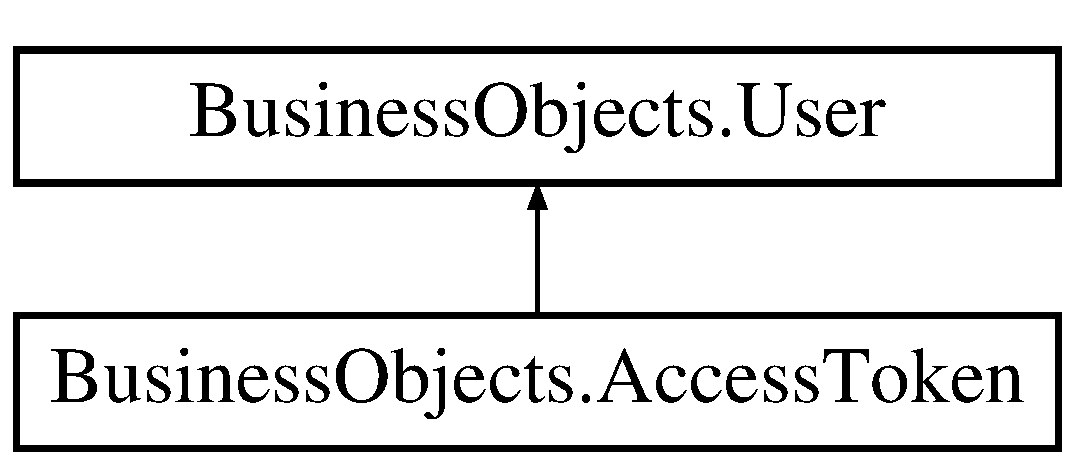
\includegraphics[height=2.000000cm]{class_business_objects_1_1_access_token}
\end{center}
\end{figure}
\subsection*{Public Member Functions}
\begin{DoxyCompactItemize}
\item 
\hyperlink{class_business_objects_1_1_access_token_a0db5c344cbe742041a0200d686df4dfe}{Access\+Token} (\hyperlink{class_business_objects_1_1_user}{User} user, List$<$ \hyperlink{class_business_objects_1_1_roles}{Roles} $>$ roles)
\begin{DoxyCompactList}\small\item\em Initializes a new instance of the \hyperlink{class_business_objects_1_1_access_token}{Access\+Token} class. \end{DoxyCompactList}\end{DoxyCompactItemize}
\subsection*{Properties}
\begin{DoxyCompactItemize}
\item 
List$<$ \hyperlink{class_business_objects_1_1_roles}{Roles} $>$ {\bfseries Roles}\hspace{0.3cm}{\ttfamily  \mbox{[}get, private set\mbox{]}}\hypertarget{class_business_objects_1_1_access_token_a5d5c41760baf531cf54bc15680357c6c}{}\label{class_business_objects_1_1_access_token_a5d5c41760baf531cf54bc15680357c6c}

\end{DoxyCompactItemize}


\subsection{Detailed Description}
\hyperlink{class_business_objects_1_1_access_token}{Access\+Token} object to hold necessary data on the user\textquotesingle{}s authentication and role status. 

\begin{DoxySeeAlso}{See also}
\hyperlink{class_business_objects_1_1_user}{Business\+Objects.\+User}


\end{DoxySeeAlso}


Definition at line 13 of file Access\+Token.\+cs.



\subsection{Constructor \& Destructor Documentation}
\index{Business\+Objects\+::\+Access\+Token@{Business\+Objects\+::\+Access\+Token}!Access\+Token@{Access\+Token}}
\index{Access\+Token@{Access\+Token}!Business\+Objects\+::\+Access\+Token@{Business\+Objects\+::\+Access\+Token}}
\subsubsection[{\texorpdfstring{Access\+Token(\+User user, List$<$ Roles $>$ roles)}{AccessToken(User user, List< Roles > roles)}}]{\setlength{\rightskip}{0pt plus 5cm}Business\+Objects.\+Access\+Token.\+Access\+Token (
\begin{DoxyParamCaption}
\item[{{\bf User}}]{user, }
\item[{List$<$ {\bf Roles} $>$}]{roles}
\end{DoxyParamCaption}
)}\hypertarget{class_business_objects_1_1_access_token_a0db5c344cbe742041a0200d686df4dfe}{}\label{class_business_objects_1_1_access_token_a0db5c344cbe742041a0200d686df4dfe}


Initializes a new instance of the \hyperlink{class_business_objects_1_1_access_token}{Access\+Token} class. 


\begin{DoxyParams}{Parameters}
{\em user} & The user.\\
\hline
{\em roles} & The roles assigned to the user.\\
\hline
\end{DoxyParams}

\begin{DoxyExceptions}{Exceptions}
{\em System.\+Application\+Exception} & Invalid \hyperlink{class_business_objects_1_1_user}{User}.\\
\hline
\end{DoxyExceptions}


Definition at line 23 of file Access\+Token.\+cs.



The documentation for this class was generated from the following file\+:\begin{DoxyCompactItemize}
\item 
C\+:/\+Users/nh228u08/\+Desktop/\+Final\+Project/\+Final\+Project/\+P\+C\+Builder/\+Business\+Objects/Access\+Token.\+cs\end{DoxyCompactItemize}

\hypertarget{class_p_c_builder_m_v_c_1_1_controllers_1_1_account_controller}{}\section{P\+C\+Builder\+M\+V\+C.\+Controllers.\+Account\+Controller Class Reference}
\label{class_p_c_builder_m_v_c_1_1_controllers_1_1_account_controller}\index{P\+C\+Builder\+M\+V\+C.\+Controllers.\+Account\+Controller@{P\+C\+Builder\+M\+V\+C.\+Controllers.\+Account\+Controller}}


Account controller to handle Account views interaction.  


Inheritance diagram for P\+C\+Builder\+M\+V\+C.\+Controllers.\+Account\+Controller\+:\begin{figure}[H]
\begin{center}
\leavevmode
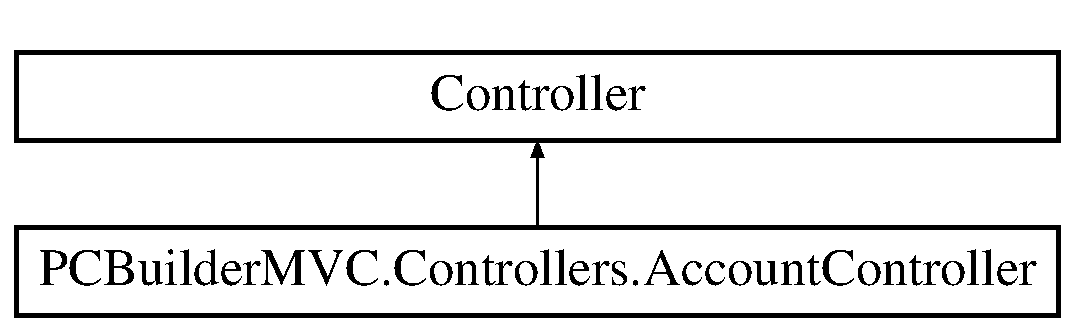
\includegraphics[height=2.000000cm]{class_p_c_builder_m_v_c_1_1_controllers_1_1_account_controller}
\end{center}
\end{figure}
\subsection*{Classes}
\begin{DoxyCompactItemize}
\item 
class \hyperlink{class_p_c_builder_m_v_c_1_1_controllers_1_1_account_controller_1_1_challenge_result}{Challenge\+Result}
\end{DoxyCompactItemize}
\subsection*{Public Types}
\begin{DoxyCompactItemize}
\item 
enum {\bfseries Manage\+Message\+Id} \{ {\bfseries Change\+Password\+Success}, 
{\bfseries Set\+Password\+Success}, 
{\bfseries Remove\+Login\+Success}, 
{\bfseries Error}
 \}\hypertarget{class_p_c_builder_m_v_c_1_1_controllers_1_1_account_controller_ad3692d193cfffaef23c5b0b72b7b69ab}{}\label{class_p_c_builder_m_v_c_1_1_controllers_1_1_account_controller_ad3692d193cfffaef23c5b0b72b7b69ab}

\end{DoxyCompactItemize}
\subsection*{Public Member Functions}
\begin{DoxyCompactItemize}
\item 
{\bfseries Account\+Controller} (\hyperlink{class_p_c_builder_m_v_c_1_1_application_user_manager}{Application\+User\+Manager} user\+Manager)\hypertarget{class_p_c_builder_m_v_c_1_1_controllers_1_1_account_controller_a3df29313acdd6591b5873bb9bdb67b71}{}\label{class_p_c_builder_m_v_c_1_1_controllers_1_1_account_controller_a3df29313acdd6591b5873bb9bdb67b71}

\item 
Action\+Result {\bfseries Login} (string return\+Url)\hypertarget{class_p_c_builder_m_v_c_1_1_controllers_1_1_account_controller_ae380c072ed2c6c2f2aa3ec143d06069a}{}\label{class_p_c_builder_m_v_c_1_1_controllers_1_1_account_controller_ae380c072ed2c6c2f2aa3ec143d06069a}

\item 
async Task$<$ Action\+Result $>$ {\bfseries Login} (\hyperlink{class_p_c_builder_m_v_c_1_1_models_1_1_login_view_model}{Login\+View\+Model} model, string return\+Url)\hypertarget{class_p_c_builder_m_v_c_1_1_controllers_1_1_account_controller_ae54dbd2be5908155b37a0c7a76bb022d}{}\label{class_p_c_builder_m_v_c_1_1_controllers_1_1_account_controller_ae54dbd2be5908155b37a0c7a76bb022d}

\item 
Action\+Result {\bfseries Register} ()\hypertarget{class_p_c_builder_m_v_c_1_1_controllers_1_1_account_controller_a92aa1b746f1a5607e2667ce98f2efed9}{}\label{class_p_c_builder_m_v_c_1_1_controllers_1_1_account_controller_a92aa1b746f1a5607e2667ce98f2efed9}

\item 
async Task$<$ Action\+Result $>$ {\bfseries Register} (\hyperlink{class_p_c_builder_m_v_c_1_1_models_1_1_register_view_model}{Register\+View\+Model} model)\hypertarget{class_p_c_builder_m_v_c_1_1_controllers_1_1_account_controller_abc856a6c8ee0bd33cff9bacee36fedfe}{}\label{class_p_c_builder_m_v_c_1_1_controllers_1_1_account_controller_abc856a6c8ee0bd33cff9bacee36fedfe}

\item 
async Task$<$ Action\+Result $>$ {\bfseries Confirm\+Email} (string user\+Id, string code)\hypertarget{class_p_c_builder_m_v_c_1_1_controllers_1_1_account_controller_a6aed0b4d63a8ff3d35b1428451a15e7b}{}\label{class_p_c_builder_m_v_c_1_1_controllers_1_1_account_controller_a6aed0b4d63a8ff3d35b1428451a15e7b}

\item 
Action\+Result {\bfseries Forgot\+Password} ()\hypertarget{class_p_c_builder_m_v_c_1_1_controllers_1_1_account_controller_a9123201fc1ab48128f5218abb3d859e0}{}\label{class_p_c_builder_m_v_c_1_1_controllers_1_1_account_controller_a9123201fc1ab48128f5218abb3d859e0}

\item 
async Task$<$ Action\+Result $>$ {\bfseries Forgot\+Password} (\hyperlink{class_p_c_builder_m_v_c_1_1_models_1_1_forgot_password_view_model}{Forgot\+Password\+View\+Model} model)\hypertarget{class_p_c_builder_m_v_c_1_1_controllers_1_1_account_controller_ad2776ab9d0b98fe8256c12d86037ddb2}{}\label{class_p_c_builder_m_v_c_1_1_controllers_1_1_account_controller_ad2776ab9d0b98fe8256c12d86037ddb2}

\item 
Action\+Result {\bfseries Forgot\+Password\+Confirmation} ()\hypertarget{class_p_c_builder_m_v_c_1_1_controllers_1_1_account_controller_a75d016c3002e245b36c3530a92d8afad}{}\label{class_p_c_builder_m_v_c_1_1_controllers_1_1_account_controller_a75d016c3002e245b36c3530a92d8afad}

\item 
Action\+Result {\bfseries Reset\+Password} (string code)\hypertarget{class_p_c_builder_m_v_c_1_1_controllers_1_1_account_controller_a8cf1eea1c767332f70226c31874e1321}{}\label{class_p_c_builder_m_v_c_1_1_controllers_1_1_account_controller_a8cf1eea1c767332f70226c31874e1321}

\item 
async Task$<$ Action\+Result $>$ {\bfseries Reset\+Password} (\hyperlink{class_p_c_builder_m_v_c_1_1_models_1_1_reset_password_view_model}{Reset\+Password\+View\+Model} model)\hypertarget{class_p_c_builder_m_v_c_1_1_controllers_1_1_account_controller_a785e97b23ad2b5effd37c12719597b03}{}\label{class_p_c_builder_m_v_c_1_1_controllers_1_1_account_controller_a785e97b23ad2b5effd37c12719597b03}

\item 
Action\+Result {\bfseries Reset\+Password\+Confirmation} ()\hypertarget{class_p_c_builder_m_v_c_1_1_controllers_1_1_account_controller_a74560e996a058eeda093d161a141c916}{}\label{class_p_c_builder_m_v_c_1_1_controllers_1_1_account_controller_a74560e996a058eeda093d161a141c916}

\item 
async Task$<$ Action\+Result $>$ {\bfseries Disassociate} (string login\+Provider, string provider\+Key)\hypertarget{class_p_c_builder_m_v_c_1_1_controllers_1_1_account_controller_a951282fe09539493acc5e0ac701125c5}{}\label{class_p_c_builder_m_v_c_1_1_controllers_1_1_account_controller_a951282fe09539493acc5e0ac701125c5}

\item 
Action\+Result {\bfseries Manage} (Manage\+Message\+Id?message)\hypertarget{class_p_c_builder_m_v_c_1_1_controllers_1_1_account_controller_a9e62c1f787a32d28bd36d95684aec9fc}{}\label{class_p_c_builder_m_v_c_1_1_controllers_1_1_account_controller_a9e62c1f787a32d28bd36d95684aec9fc}

\item 
async Task$<$ Action\+Result $>$ {\bfseries Manage} (\hyperlink{class_p_c_builder_m_v_c_1_1_models_1_1_manage_user_view_model}{Manage\+User\+View\+Model} model)\hypertarget{class_p_c_builder_m_v_c_1_1_controllers_1_1_account_controller_aa54468166a91284e9ab801c6c93735be}{}\label{class_p_c_builder_m_v_c_1_1_controllers_1_1_account_controller_aa54468166a91284e9ab801c6c93735be}

\item 
Action\+Result {\bfseries External\+Login} (string provider, string return\+Url)\hypertarget{class_p_c_builder_m_v_c_1_1_controllers_1_1_account_controller_a7b9f58ec5691d7e5432aa85caabdce1a}{}\label{class_p_c_builder_m_v_c_1_1_controllers_1_1_account_controller_a7b9f58ec5691d7e5432aa85caabdce1a}

\item 
async Task$<$ Action\+Result $>$ {\bfseries External\+Login\+Callback} (string return\+Url)\hypertarget{class_p_c_builder_m_v_c_1_1_controllers_1_1_account_controller_aca010e9588956c6fcf9fd40992f8a9d5}{}\label{class_p_c_builder_m_v_c_1_1_controllers_1_1_account_controller_aca010e9588956c6fcf9fd40992f8a9d5}

\item 
Action\+Result {\bfseries Link\+Login} (string provider)\hypertarget{class_p_c_builder_m_v_c_1_1_controllers_1_1_account_controller_af4463ae5ae9ebdd71a7921459241af89}{}\label{class_p_c_builder_m_v_c_1_1_controllers_1_1_account_controller_af4463ae5ae9ebdd71a7921459241af89}

\item 
async Task$<$ Action\+Result $>$ {\bfseries Link\+Login\+Callback} ()\hypertarget{class_p_c_builder_m_v_c_1_1_controllers_1_1_account_controller_a5464ab822361c3aae7ea11b71afb2833}{}\label{class_p_c_builder_m_v_c_1_1_controllers_1_1_account_controller_a5464ab822361c3aae7ea11b71afb2833}

\item 
async Task$<$ Action\+Result $>$ {\bfseries External\+Login\+Confirmation} (\hyperlink{class_p_c_builder_m_v_c_1_1_models_1_1_external_login_confirmation_view_model}{External\+Login\+Confirmation\+View\+Model} model, string return\+Url)\hypertarget{class_p_c_builder_m_v_c_1_1_controllers_1_1_account_controller_a3e8a615f61a8cb1260ad3d1eeec2aa41}{}\label{class_p_c_builder_m_v_c_1_1_controllers_1_1_account_controller_a3e8a615f61a8cb1260ad3d1eeec2aa41}

\item 
Action\+Result {\bfseries Log\+Off} ()\hypertarget{class_p_c_builder_m_v_c_1_1_controllers_1_1_account_controller_a1e8962ce6f6e6b413c0e4aa54ee8ff4e}{}\label{class_p_c_builder_m_v_c_1_1_controllers_1_1_account_controller_a1e8962ce6f6e6b413c0e4aa54ee8ff4e}

\item 
Action\+Result {\bfseries External\+Login\+Failure} ()\hypertarget{class_p_c_builder_m_v_c_1_1_controllers_1_1_account_controller_a98f2769b65d47f2eecf8de39e891a477}{}\label{class_p_c_builder_m_v_c_1_1_controllers_1_1_account_controller_a98f2769b65d47f2eecf8de39e891a477}

\item 
Action\+Result {\bfseries Remove\+Account\+List} ()\hypertarget{class_p_c_builder_m_v_c_1_1_controllers_1_1_account_controller_aacd25e3088db5d4fa258f686eb71c299}{}\label{class_p_c_builder_m_v_c_1_1_controllers_1_1_account_controller_aacd25e3088db5d4fa258f686eb71c299}

\end{DoxyCompactItemize}
\subsection*{Protected Member Functions}
\begin{DoxyCompactItemize}
\item 
override void {\bfseries Dispose} (bool disposing)\hypertarget{class_p_c_builder_m_v_c_1_1_controllers_1_1_account_controller_a61fac6a43b44896e9ed7879a51a1c487}{}\label{class_p_c_builder_m_v_c_1_1_controllers_1_1_account_controller_a61fac6a43b44896e9ed7879a51a1c487}

\end{DoxyCompactItemize}
\subsection*{Properties}
\begin{DoxyCompactItemize}
\item 
\hyperlink{class_p_c_builder_m_v_c_1_1_application_user_manager}{Application\+User\+Manager} {\bfseries User\+Manager}\hspace{0.3cm}{\ttfamily  \mbox{[}get, private set\mbox{]}}\hypertarget{class_p_c_builder_m_v_c_1_1_controllers_1_1_account_controller_a7bfd8964878a6c640b079f81641ebed6}{}\label{class_p_c_builder_m_v_c_1_1_controllers_1_1_account_controller_a7bfd8964878a6c640b079f81641ebed6}

\item 
I\+Authentication\+Manager {\bfseries Authentication\+Manager}\hspace{0.3cm}{\ttfamily  \mbox{[}get\mbox{]}}\hypertarget{class_p_c_builder_m_v_c_1_1_controllers_1_1_account_controller_a4fe85c110c5c3dede8d55b27fcadaa3f}{}\label{class_p_c_builder_m_v_c_1_1_controllers_1_1_account_controller_a4fe85c110c5c3dede8d55b27fcadaa3f}

\end{DoxyCompactItemize}
\subsection*{Private Member Functions}
\begin{DoxyCompactItemize}
\item 
async Task {\bfseries Sign\+In\+Async} (\hyperlink{class_p_c_builder_m_v_c_1_1_models_1_1_application_user}{Application\+User} user, bool is\+Persistent)\hypertarget{class_p_c_builder_m_v_c_1_1_controllers_1_1_account_controller_afb3adb4d6e2dd57c0551e4853abd26fe}{}\label{class_p_c_builder_m_v_c_1_1_controllers_1_1_account_controller_afb3adb4d6e2dd57c0551e4853abd26fe}

\item 
void {\bfseries Add\+Errors} (Identity\+Result result)\hypertarget{class_p_c_builder_m_v_c_1_1_controllers_1_1_account_controller_a6ebea49c8114af9e18f742c7f57ce7a6}{}\label{class_p_c_builder_m_v_c_1_1_controllers_1_1_account_controller_a6ebea49c8114af9e18f742c7f57ce7a6}

\item 
bool {\bfseries Has\+Password} ()\hypertarget{class_p_c_builder_m_v_c_1_1_controllers_1_1_account_controller_a0520a211ff47b1b31296215a75b2edd8}{}\label{class_p_c_builder_m_v_c_1_1_controllers_1_1_account_controller_a0520a211ff47b1b31296215a75b2edd8}

\item 
void {\bfseries Send\+Email} (string email, string callback\+Url, string subject, string message)\hypertarget{class_p_c_builder_m_v_c_1_1_controllers_1_1_account_controller_a21e5ebc02425bba4b3d2eef5bc47447a}{}\label{class_p_c_builder_m_v_c_1_1_controllers_1_1_account_controller_a21e5ebc02425bba4b3d2eef5bc47447a}

\item 
Action\+Result {\bfseries Redirect\+To\+Local} (string return\+Url)\hypertarget{class_p_c_builder_m_v_c_1_1_controllers_1_1_account_controller_a68ee6edabbc6c6090bd29c59797e0e0c}{}\label{class_p_c_builder_m_v_c_1_1_controllers_1_1_account_controller_a68ee6edabbc6c6090bd29c59797e0e0c}

\end{DoxyCompactItemize}
\subsection*{Private Attributes}
\begin{DoxyCompactItemize}
\item 
\hyperlink{class_p_c_builder_m_v_c_1_1_application_user_manager}{Application\+User\+Manager} {\bfseries \+\_\+user\+Manager}\hypertarget{class_p_c_builder_m_v_c_1_1_controllers_1_1_account_controller_ac6da80aa091b402afa58aaad261523b8}{}\label{class_p_c_builder_m_v_c_1_1_controllers_1_1_account_controller_ac6da80aa091b402afa58aaad261523b8}

\item 
const string {\bfseries Xsrf\+Key} = \char`\"{}Xsrf\+Id\char`\"{}\hypertarget{class_p_c_builder_m_v_c_1_1_controllers_1_1_account_controller_a618e736b98df1dc62c90859c37b19312}{}\label{class_p_c_builder_m_v_c_1_1_controllers_1_1_account_controller_a618e736b98df1dc62c90859c37b19312}

\end{DoxyCompactItemize}


\subsection{Detailed Description}
Account controller to handle Account views interaction. 

\begin{DoxySeeAlso}{See also}
System.\+Web.\+Mvc.\+Controller


\end{DoxySeeAlso}


Definition at line 22 of file Account\+Controller.\+cs.



The documentation for this class was generated from the following file\+:\begin{DoxyCompactItemize}
\item 
C\+:/\+Users/nh228u08/\+Desktop/\+Final\+Project/\+Final\+Project/\+P\+C\+Builder/\+P\+C\+Builder\+M\+V\+C/\+Controllers/Account\+Controller.\+cs\end{DoxyCompactItemize}

\hypertarget{class_p_c_builder_m_v_c_1_1_controllers_1_1_administration_controller}{}\section{P\+C\+Builder\+M\+V\+C.\+Controllers.\+Administration\+Controller Class Reference}
\label{class_p_c_builder_m_v_c_1_1_controllers_1_1_administration_controller}\index{P\+C\+Builder\+M\+V\+C.\+Controllers.\+Administration\+Controller@{P\+C\+Builder\+M\+V\+C.\+Controllers.\+Administration\+Controller}}


Administrator controller class to handle Administrator views interaction.  


Inheritance diagram for P\+C\+Builder\+M\+V\+C.\+Controllers.\+Administration\+Controller\+:\begin{figure}[H]
\begin{center}
\leavevmode
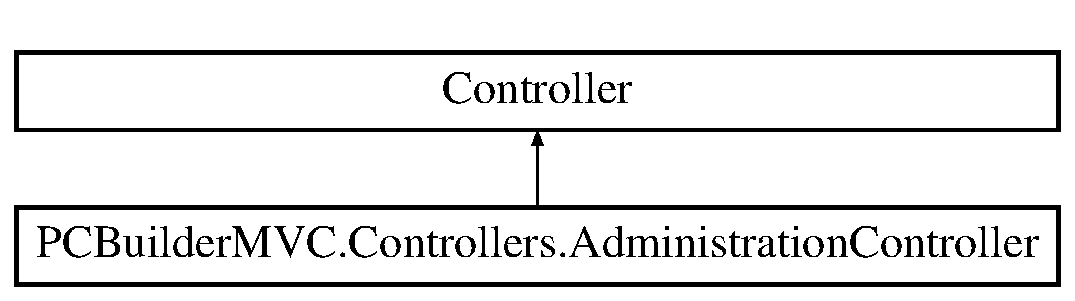
\includegraphics[height=2.000000cm]{class_p_c_builder_m_v_c_1_1_controllers_1_1_administration_controller}
\end{center}
\end{figure}
\subsection*{Public Member Functions}
\begin{DoxyCompactItemize}
\item 
Action\+Result {\bfseries Index} ()\hypertarget{class_p_c_builder_m_v_c_1_1_controllers_1_1_administration_controller_a7f1898706308a45f6d458613efa5365e}{}\label{class_p_c_builder_m_v_c_1_1_controllers_1_1_administration_controller_a7f1898706308a45f6d458613efa5365e}

\end{DoxyCompactItemize}


\subsection{Detailed Description}
Administrator controller class to handle Administrator views interaction. 

\begin{DoxySeeAlso}{See also}
System.\+Web.\+Mvc.\+Controller


\end{DoxySeeAlso}


Definition at line 14 of file Administration\+Controller.\+cs.



The documentation for this class was generated from the following file\+:\begin{DoxyCompactItemize}
\item 
C\+:/\+Users/nh228u08/\+Desktop/\+Final\+Project/\+Final\+Project/\+P\+C\+Builder/\+P\+C\+Builder\+M\+V\+C/\+Controllers/Administration\+Controller.\+cs\end{DoxyCompactItemize}

\hypertarget{class_p_c_builder_forms_1_1_app}{}\section{P\+C\+Builder\+Forms.\+App Class Reference}
\label{class_p_c_builder_forms_1_1_app}\index{P\+C\+Builder\+Forms.\+App@{P\+C\+Builder\+Forms.\+App}}


Interaction logic for App.\+xaml  


Inheritance diagram for P\+C\+Builder\+Forms.\+App\+:\begin{figure}[H]
\begin{center}
\leavevmode
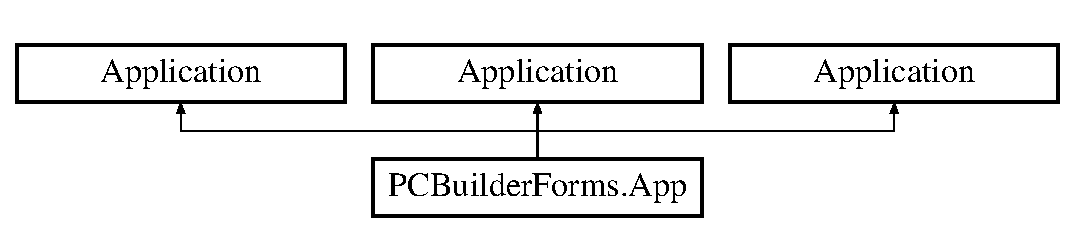
\includegraphics[height=2.000000cm]{class_p_c_builder_forms_1_1_app}
\end{center}
\end{figure}
\subsection*{Public Member Functions}
\begin{DoxyCompactItemize}
\item 
void \hyperlink{class_p_c_builder_forms_1_1_app_af10a7f8ea27debb593e600d4b7e0550e}{Initialize\+Component} ()
\begin{DoxyCompactList}\small\item\em Initialize\+Component \end{DoxyCompactList}\item 
void \hyperlink{class_p_c_builder_forms_1_1_app_af10a7f8ea27debb593e600d4b7e0550e}{Initialize\+Component} ()
\begin{DoxyCompactList}\small\item\em Initialize\+Component \end{DoxyCompactList}\end{DoxyCompactItemize}
\subsection*{Static Public Member Functions}
\begin{DoxyCompactItemize}
\item 
static void \hyperlink{class_p_c_builder_forms_1_1_app_a8e0e2ce98707651cc8d9f09d9866f51a}{Main} ()
\begin{DoxyCompactList}\small\item\em Application Entry Point. \end{DoxyCompactList}\item 
static void \hyperlink{class_p_c_builder_forms_1_1_app_a8e0e2ce98707651cc8d9f09d9866f51a}{Main} ()
\begin{DoxyCompactList}\small\item\em Application Entry Point. \end{DoxyCompactList}\end{DoxyCompactItemize}


\subsection{Detailed Description}
Interaction logic for App.\+xaml 

\hyperlink{class_p_c_builder_forms_1_1_app}{App} 

Definition at line 14 of file App.\+xaml.\+cs.



\subsection{Member Function Documentation}
\index{P\+C\+Builder\+Forms\+::\+App@{P\+C\+Builder\+Forms\+::\+App}!Initialize\+Component@{Initialize\+Component}}
\index{Initialize\+Component@{Initialize\+Component}!P\+C\+Builder\+Forms\+::\+App@{P\+C\+Builder\+Forms\+::\+App}}
\subsubsection[{\texorpdfstring{Initialize\+Component()}{InitializeComponent()}}]{\setlength{\rightskip}{0pt plus 5cm}void P\+C\+Builder\+Forms.\+App.\+Initialize\+Component (
\begin{DoxyParamCaption}
{}
\end{DoxyParamCaption}
)}\hypertarget{class_p_c_builder_forms_1_1_app_af10a7f8ea27debb593e600d4b7e0550e}{}\label{class_p_c_builder_forms_1_1_app_af10a7f8ea27debb593e600d4b7e0550e}


Initialize\+Component 



Definition at line 48 of file App.\+g.\+cs.

\index{P\+C\+Builder\+Forms\+::\+App@{P\+C\+Builder\+Forms\+::\+App}!Initialize\+Component@{Initialize\+Component}}
\index{Initialize\+Component@{Initialize\+Component}!P\+C\+Builder\+Forms\+::\+App@{P\+C\+Builder\+Forms\+::\+App}}
\subsubsection[{\texorpdfstring{Initialize\+Component()}{InitializeComponent()}}]{\setlength{\rightskip}{0pt plus 5cm}void P\+C\+Builder\+Forms.\+App.\+Initialize\+Component (
\begin{DoxyParamCaption}
{}
\end{DoxyParamCaption}
)}\hypertarget{class_p_c_builder_forms_1_1_app_af10a7f8ea27debb593e600d4b7e0550e}{}\label{class_p_c_builder_forms_1_1_app_af10a7f8ea27debb593e600d4b7e0550e}


Initialize\+Component 



Definition at line 48 of file App.\+g.\+i.\+cs.

\index{P\+C\+Builder\+Forms\+::\+App@{P\+C\+Builder\+Forms\+::\+App}!Main@{Main}}
\index{Main@{Main}!P\+C\+Builder\+Forms\+::\+App@{P\+C\+Builder\+Forms\+::\+App}}
\subsubsection[{\texorpdfstring{Main()}{Main()}}]{\setlength{\rightskip}{0pt plus 5cm}static void P\+C\+Builder\+Forms.\+App.\+Main (
\begin{DoxyParamCaption}
{}
\end{DoxyParamCaption}
)\hspace{0.3cm}{\ttfamily [static]}}\hypertarget{class_p_c_builder_forms_1_1_app_a8e0e2ce98707651cc8d9f09d9866f51a}{}\label{class_p_c_builder_forms_1_1_app_a8e0e2ce98707651cc8d9f09d9866f51a}


Application Entry Point. 



Definition at line 63 of file App.\+g.\+i.\+cs.

\index{P\+C\+Builder\+Forms\+::\+App@{P\+C\+Builder\+Forms\+::\+App}!Main@{Main}}
\index{Main@{Main}!P\+C\+Builder\+Forms\+::\+App@{P\+C\+Builder\+Forms\+::\+App}}
\subsubsection[{\texorpdfstring{Main()}{Main()}}]{\setlength{\rightskip}{0pt plus 5cm}static void P\+C\+Builder\+Forms.\+App.\+Main (
\begin{DoxyParamCaption}
{}
\end{DoxyParamCaption}
)\hspace{0.3cm}{\ttfamily [static]}}\hypertarget{class_p_c_builder_forms_1_1_app_a8e0e2ce98707651cc8d9f09d9866f51a}{}\label{class_p_c_builder_forms_1_1_app_a8e0e2ce98707651cc8d9f09d9866f51a}


Application Entry Point. 



Definition at line 63 of file App.\+g.\+cs.



The documentation for this class was generated from the following files\+:\begin{DoxyCompactItemize}
\item 
C\+:/\+Users/nh228u08/\+Desktop/\+Final\+Project/\+Final\+Project/\+P\+C\+Builder/\+P\+C\+Builder\+Forms/App.\+xaml.\+cs\item 
C\+:/\+Users/nh228u08/\+Desktop/\+Final\+Project/\+Final\+Project/\+P\+C\+Builder/\+P\+C\+Builder\+Forms/obj/\+Debug/App.\+g.\+cs\item 
C\+:/\+Users/nh228u08/\+Desktop/\+Final\+Project/\+Final\+Project/\+P\+C\+Builder/\+P\+C\+Builder\+Forms/obj/\+Debug/App.\+g.\+i.\+cs\end{DoxyCompactItemize}

\hypertarget{class_p_c_builder_m_v_c_1_1_models_1_1_application_db_context}{}\section{P\+C\+Builder\+M\+V\+C.\+Models.\+Application\+Db\+Context Class Reference}
\label{class_p_c_builder_m_v_c_1_1_models_1_1_application_db_context}\index{P\+C\+Builder\+M\+V\+C.\+Models.\+Application\+Db\+Context@{P\+C\+Builder\+M\+V\+C.\+Models.\+Application\+Db\+Context}}


Database connection for \hyperlink{class_p_c_builder_m_v_c_1_1_models_1_1_user}{User} model.  


Inheritance diagram for P\+C\+Builder\+M\+V\+C.\+Models.\+Application\+Db\+Context\+:\begin{figure}[H]
\begin{center}
\leavevmode
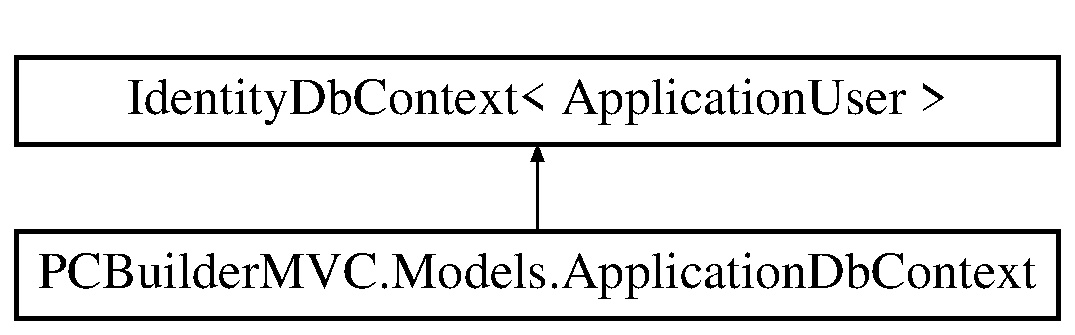
\includegraphics[height=2.000000cm]{class_p_c_builder_m_v_c_1_1_models_1_1_application_db_context}
\end{center}
\end{figure}
\subsection*{Static Public Member Functions}
\begin{DoxyCompactItemize}
\item 
static \hyperlink{class_p_c_builder_m_v_c_1_1_models_1_1_application_db_context}{Application\+Db\+Context} {\bfseries Create} ()\hypertarget{class_p_c_builder_m_v_c_1_1_models_1_1_application_db_context_a87e83c7a94db34abb35a1e6d7df4c6e3}{}\label{class_p_c_builder_m_v_c_1_1_models_1_1_application_db_context_a87e83c7a94db34abb35a1e6d7df4c6e3}

\end{DoxyCompactItemize}
\subsection*{Properties}
\begin{DoxyCompactItemize}
\item 
System.\+Data.\+Entity.\+Db\+Set$<$ \hyperlink{class_p_c_builder_m_v_c_1_1_models_1_1_c_p_u}{P\+C\+Builder\+M\+V\+C.\+Models.\+C\+PU} $>$ {\bfseries C\+P\+Us}\hspace{0.3cm}{\ttfamily  \mbox{[}get, set\mbox{]}}\hypertarget{class_p_c_builder_m_v_c_1_1_models_1_1_application_db_context_abe6c40c6be3a6fd178405e5dcc7a5b7f}{}\label{class_p_c_builder_m_v_c_1_1_models_1_1_application_db_context_abe6c40c6be3a6fd178405e5dcc7a5b7f}

\item 
System.\+Data.\+Entity.\+Db\+Set$<$ \hyperlink{class_p_c_builder_m_v_c_1_1_models_1_1_asp_net_role}{P\+C\+Builder\+M\+V\+C.\+Models.\+Asp\+Net\+Role} $>$ {\bfseries Asp\+Net\+Roles}\hspace{0.3cm}{\ttfamily  \mbox{[}get, set\mbox{]}}\hypertarget{class_p_c_builder_m_v_c_1_1_models_1_1_application_db_context_a3999bd7ef81ac8511b08b2b067744c1a}{}\label{class_p_c_builder_m_v_c_1_1_models_1_1_application_db_context_a3999bd7ef81ac8511b08b2b067744c1a}

\end{DoxyCompactItemize}


\subsection{Detailed Description}
Database connection for \hyperlink{class_p_c_builder_m_v_c_1_1_models_1_1_user}{User} model. 

\begin{DoxySeeAlso}{See also}
Microsoft.\+Asp\+Net.\+Identity.\+Entity\+Framework.\+Identity\+Db\+Context$<$\+P\+C\+Builder\+M\+V\+C.\+Models.\+Application\+User$>$


\end{DoxySeeAlso}


Definition at line 28 of file Identity\+Models.\+cs.



The documentation for this class was generated from the following file\+:\begin{DoxyCompactItemize}
\item 
C\+:/\+Users/nh228u08/\+Desktop/\+Final\+Project/\+Final\+Project/\+P\+C\+Builder/\+P\+C\+Builder\+M\+V\+C/\+Models/Identity\+Models.\+cs\end{DoxyCompactItemize}

\hypertarget{class_p_c_builder_m_v_c_1_1_models_1_1_application_user}{}\section{P\+C\+Builder\+M\+V\+C.\+Models.\+Application\+User Class Reference}
\label{class_p_c_builder_m_v_c_1_1_models_1_1_application_user}\index{P\+C\+Builder\+M\+V\+C.\+Models.\+Application\+User@{P\+C\+Builder\+M\+V\+C.\+Models.\+Application\+User}}


Application user model.  


Inheritance diagram for P\+C\+Builder\+M\+V\+C.\+Models.\+Application\+User\+:\begin{figure}[H]
\begin{center}
\leavevmode
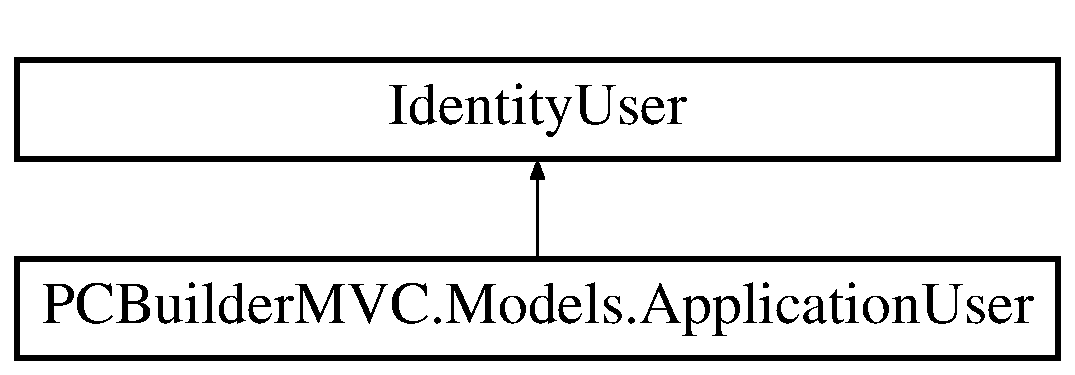
\includegraphics[height=2.000000cm]{class_p_c_builder_m_v_c_1_1_models_1_1_application_user}
\end{center}
\end{figure}
\subsection*{Public Member Functions}
\begin{DoxyCompactItemize}
\item 
async Task$<$ Claims\+Identity $>$ {\bfseries Generate\+User\+Identity\+Async} (User\+Manager$<$ \hyperlink{class_p_c_builder_m_v_c_1_1_models_1_1_application_user}{Application\+User} $>$ manager)\hypertarget{class_p_c_builder_m_v_c_1_1_models_1_1_application_user_a1958c9bf9604c202bc00ed69dd0425e4}{}\label{class_p_c_builder_m_v_c_1_1_models_1_1_application_user_a1958c9bf9604c202bc00ed69dd0425e4}

\end{DoxyCompactItemize}


\subsection{Detailed Description}
Application user model. 

\begin{DoxySeeAlso}{See also}
Microsoft.\+Asp\+Net.\+Identity.\+Entity\+Framework.\+Identity\+User


\end{DoxySeeAlso}


Definition at line 13 of file Identity\+Models.\+cs.



The documentation for this class was generated from the following file\+:\begin{DoxyCompactItemize}
\item 
C\+:/\+Users/nh228u08/\+Desktop/\+Final\+Project/\+Final\+Project/\+P\+C\+Builder/\+P\+C\+Builder\+M\+V\+C/\+Models/Identity\+Models.\+cs\end{DoxyCompactItemize}

\hypertarget{class_p_c_builder_m_v_c_1_1_application_user_manager}{}\section{P\+C\+Builder\+M\+V\+C.\+Application\+User\+Manager Class Reference}
\label{class_p_c_builder_m_v_c_1_1_application_user_manager}\index{P\+C\+Builder\+M\+V\+C.\+Application\+User\+Manager@{P\+C\+Builder\+M\+V\+C.\+Application\+User\+Manager}}


User manager for the M\+VC project.  


Inheritance diagram for P\+C\+Builder\+M\+V\+C.\+Application\+User\+Manager\+:\begin{figure}[H]
\begin{center}
\leavevmode
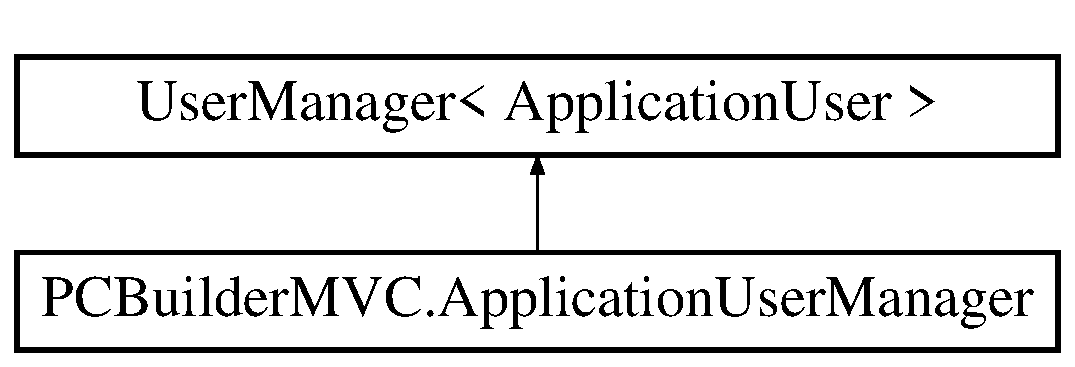
\includegraphics[height=2.000000cm]{class_p_c_builder_m_v_c_1_1_application_user_manager}
\end{center}
\end{figure}
\subsection*{Public Member Functions}
\begin{DoxyCompactItemize}
\item 
\hyperlink{class_p_c_builder_m_v_c_1_1_application_user_manager_af4a41b30be1457d972406354e95fb945}{Application\+User\+Manager} (I\+User\+Store$<$ \hyperlink{class_p_c_builder_m_v_c_1_1_models_1_1_application_user}{Application\+User} $>$ store)
\begin{DoxyCompactList}\small\item\em Initializes a new instance of the \hyperlink{class_p_c_builder_m_v_c_1_1_application_user_manager}{Application\+User\+Manager} class. \end{DoxyCompactList}\end{DoxyCompactItemize}
\subsection*{Static Public Member Functions}
\begin{DoxyCompactItemize}
\item 
static \hyperlink{class_p_c_builder_m_v_c_1_1_application_user_manager}{Application\+User\+Manager} \hyperlink{class_p_c_builder_m_v_c_1_1_application_user_manager_abf2e4bf064febf08f995528ce52545b5}{Create} (Identity\+Factory\+Options$<$ \hyperlink{class_p_c_builder_m_v_c_1_1_application_user_manager}{Application\+User\+Manager} $>$ options, I\+Owin\+Context context)
\begin{DoxyCompactList}\small\item\em Creates the specified options. \end{DoxyCompactList}\end{DoxyCompactItemize}


\subsection{Detailed Description}
User manager for the M\+VC project. 

\begin{DoxySeeAlso}{See also}
Microsoft.\+Asp\+Net.\+Identity.\+User\+Manager$<$\+P\+C\+Builder\+M\+V\+C.\+Models.\+Application\+User$>$


\end{DoxySeeAlso}


Definition at line 16 of file Identity\+Config.\+cs.



\subsection{Constructor \& Destructor Documentation}
\index{P\+C\+Builder\+M\+V\+C\+::\+Application\+User\+Manager@{P\+C\+Builder\+M\+V\+C\+::\+Application\+User\+Manager}!Application\+User\+Manager@{Application\+User\+Manager}}
\index{Application\+User\+Manager@{Application\+User\+Manager}!P\+C\+Builder\+M\+V\+C\+::\+Application\+User\+Manager@{P\+C\+Builder\+M\+V\+C\+::\+Application\+User\+Manager}}
\subsubsection[{\texorpdfstring{Application\+User\+Manager(\+I\+User\+Store$<$ Application\+User $>$ store)}{ApplicationUserManager(IUserStore< ApplicationUser > store)}}]{\setlength{\rightskip}{0pt plus 5cm}P\+C\+Builder\+M\+V\+C.\+Application\+User\+Manager.\+Application\+User\+Manager (
\begin{DoxyParamCaption}
\item[{I\+User\+Store$<$ {\bf Application\+User} $>$}]{store}
\end{DoxyParamCaption}
)}\hypertarget{class_p_c_builder_m_v_c_1_1_application_user_manager_af4a41b30be1457d972406354e95fb945}{}\label{class_p_c_builder_m_v_c_1_1_application_user_manager_af4a41b30be1457d972406354e95fb945}


Initializes a new instance of the \hyperlink{class_p_c_builder_m_v_c_1_1_application_user_manager}{Application\+User\+Manager} class. 


\begin{DoxyParams}{Parameters}
{\em store} & The store.\\
\hline
\end{DoxyParams}


Definition at line 22 of file Identity\+Config.\+cs.



\subsection{Member Function Documentation}
\index{P\+C\+Builder\+M\+V\+C\+::\+Application\+User\+Manager@{P\+C\+Builder\+M\+V\+C\+::\+Application\+User\+Manager}!Create@{Create}}
\index{Create@{Create}!P\+C\+Builder\+M\+V\+C\+::\+Application\+User\+Manager@{P\+C\+Builder\+M\+V\+C\+::\+Application\+User\+Manager}}
\subsubsection[{\texorpdfstring{Create(\+Identity\+Factory\+Options$<$ Application\+User\+Manager $>$ options, I\+Owin\+Context context)}{Create(IdentityFactoryOptions< ApplicationUserManager > options, IOwinContext context)}}]{\setlength{\rightskip}{0pt plus 5cm}static {\bf Application\+User\+Manager} P\+C\+Builder\+M\+V\+C.\+Application\+User\+Manager.\+Create (
\begin{DoxyParamCaption}
\item[{Identity\+Factory\+Options$<$ {\bf Application\+User\+Manager} $>$}]{options, }
\item[{I\+Owin\+Context}]{context}
\end{DoxyParamCaption}
)\hspace{0.3cm}{\ttfamily [static]}}\hypertarget{class_p_c_builder_m_v_c_1_1_application_user_manager_abf2e4bf064febf08f995528ce52545b5}{}\label{class_p_c_builder_m_v_c_1_1_application_user_manager_abf2e4bf064febf08f995528ce52545b5}


Creates the specified options. 


\begin{DoxyParams}{Parameters}
{\em options} & The options.\\
\hline
{\em context} & The context.\\
\hline
\end{DoxyParams}
\begin{DoxyReturn}{Returns}

\end{DoxyReturn}


Definition at line 33 of file Identity\+Config.\+cs.



The documentation for this class was generated from the following file\+:\begin{DoxyCompactItemize}
\item 
C\+:/\+Users/nh228u08/\+Desktop/\+Final\+Project/\+Final\+Project/\+P\+C\+Builder/\+P\+C\+Builder\+M\+V\+C/\+App\+\_\+\+Start/Identity\+Config.\+cs\end{DoxyCompactItemize}

\hypertarget{class_p_c_builder_m_v_c_1_1_models_1_1_asp_net_role}{}\section{P\+C\+Builder\+M\+V\+C.\+Models.\+Asp\+Net\+Role Class Reference}
\label{class_p_c_builder_m_v_c_1_1_models_1_1_asp_net_role}\index{P\+C\+Builder\+M\+V\+C.\+Models.\+Asp\+Net\+Role@{P\+C\+Builder\+M\+V\+C.\+Models.\+Asp\+Net\+Role}}
\subsection*{Properties}
\begin{DoxyCompactItemize}
\item 
string {\bfseries Id}\hspace{0.3cm}{\ttfamily  \mbox{[}get, set\mbox{]}}\hypertarget{class_p_c_builder_m_v_c_1_1_models_1_1_asp_net_role_a06103ace45910d89ab2a844dd4ceefbe}{}\label{class_p_c_builder_m_v_c_1_1_models_1_1_asp_net_role_a06103ace45910d89ab2a844dd4ceefbe}

\item 
string {\bfseries Name}\hspace{0.3cm}{\ttfamily  \mbox{[}get, set\mbox{]}}\hypertarget{class_p_c_builder_m_v_c_1_1_models_1_1_asp_net_role_a027709b9d667d4d19f208f24e4fcdc03}{}\label{class_p_c_builder_m_v_c_1_1_models_1_1_asp_net_role_a027709b9d667d4d19f208f24e4fcdc03}

\item 
virtual I\+Collection$<$ \hyperlink{class_p_c_builder_m_v_c_1_1_models_1_1_asp_net_user}{Asp\+Net\+User} $>$ {\bfseries Asp\+Net\+Users}\hspace{0.3cm}{\ttfamily  \mbox{[}get, set\mbox{]}}\hypertarget{class_p_c_builder_m_v_c_1_1_models_1_1_asp_net_role_acee25350de7a4524f3d075d7f214ea31}{}\label{class_p_c_builder_m_v_c_1_1_models_1_1_asp_net_role_acee25350de7a4524f3d075d7f214ea31}

\end{DoxyCompactItemize}


\subsection{Detailed Description}


Definition at line 9 of file Asp\+Net\+Role.\+cs.



The documentation for this class was generated from the following file\+:\begin{DoxyCompactItemize}
\item 
C\+:/\+Users/nh228u08/\+Desktop/\+Final\+Project/\+Final\+Project/\+P\+C\+Builder/\+P\+C\+Builder\+M\+V\+C/\+Models/Asp\+Net\+Role.\+cs\end{DoxyCompactItemize}

\hypertarget{class_p_c_builder_m_v_c_1_1_models_1_1_asp_net_user}{}\section{P\+C\+Builder\+M\+V\+C.\+Models.\+Asp\+Net\+User Class Reference}
\label{class_p_c_builder_m_v_c_1_1_models_1_1_asp_net_user}\index{P\+C\+Builder\+M\+V\+C.\+Models.\+Asp\+Net\+User@{P\+C\+Builder\+M\+V\+C.\+Models.\+Asp\+Net\+User}}
\subsection*{Properties}
\begin{DoxyCompactItemize}
\item 
string {\bfseries Id}\hspace{0.3cm}{\ttfamily  \mbox{[}get, set\mbox{]}}\hypertarget{class_p_c_builder_m_v_c_1_1_models_1_1_asp_net_user_a90fbe4981800475e56eaa613862f24e1}{}\label{class_p_c_builder_m_v_c_1_1_models_1_1_asp_net_user_a90fbe4981800475e56eaa613862f24e1}

\item 
string {\bfseries Email}\hspace{0.3cm}{\ttfamily  \mbox{[}get, set\mbox{]}}\hypertarget{class_p_c_builder_m_v_c_1_1_models_1_1_asp_net_user_a4cc78fad14702a22cdac76ec509a0027}{}\label{class_p_c_builder_m_v_c_1_1_models_1_1_asp_net_user_a4cc78fad14702a22cdac76ec509a0027}

\item 
bool {\bfseries Email\+Confirmed}\hspace{0.3cm}{\ttfamily  \mbox{[}get, set\mbox{]}}\hypertarget{class_p_c_builder_m_v_c_1_1_models_1_1_asp_net_user_a25e057f79a8f118f0f3aedbd4f814100}{}\label{class_p_c_builder_m_v_c_1_1_models_1_1_asp_net_user_a25e057f79a8f118f0f3aedbd4f814100}

\item 
string {\bfseries Password\+Hash}\hspace{0.3cm}{\ttfamily  \mbox{[}get, set\mbox{]}}\hypertarget{class_p_c_builder_m_v_c_1_1_models_1_1_asp_net_user_a8c7f19af5fd87f87a9de0bbf0cad70b4}{}\label{class_p_c_builder_m_v_c_1_1_models_1_1_asp_net_user_a8c7f19af5fd87f87a9de0bbf0cad70b4}

\item 
string {\bfseries Security\+Stamp}\hspace{0.3cm}{\ttfamily  \mbox{[}get, set\mbox{]}}\hypertarget{class_p_c_builder_m_v_c_1_1_models_1_1_asp_net_user_a4ce9973b3197d4df7afceb114de1ed02}{}\label{class_p_c_builder_m_v_c_1_1_models_1_1_asp_net_user_a4ce9973b3197d4df7afceb114de1ed02}

\item 
string {\bfseries Phone\+Number}\hspace{0.3cm}{\ttfamily  \mbox{[}get, set\mbox{]}}\hypertarget{class_p_c_builder_m_v_c_1_1_models_1_1_asp_net_user_ac7c0f6805d8b63e8abd8f65974a61e6a}{}\label{class_p_c_builder_m_v_c_1_1_models_1_1_asp_net_user_ac7c0f6805d8b63e8abd8f65974a61e6a}

\item 
bool {\bfseries Phone\+Number\+Confirmed}\hspace{0.3cm}{\ttfamily  \mbox{[}get, set\mbox{]}}\hypertarget{class_p_c_builder_m_v_c_1_1_models_1_1_asp_net_user_a568b46a09dfeed9358947aa86918b436}{}\label{class_p_c_builder_m_v_c_1_1_models_1_1_asp_net_user_a568b46a09dfeed9358947aa86918b436}

\item 
bool {\bfseries Two\+Factor\+Enabled}\hspace{0.3cm}{\ttfamily  \mbox{[}get, set\mbox{]}}\hypertarget{class_p_c_builder_m_v_c_1_1_models_1_1_asp_net_user_a110b3fe4ae21ec55c2de2f0a9060a45f}{}\label{class_p_c_builder_m_v_c_1_1_models_1_1_asp_net_user_a110b3fe4ae21ec55c2de2f0a9060a45f}

\item 
Date\+Time {\bfseries Lockout\+End\+Date\+Utc}\hspace{0.3cm}{\ttfamily  \mbox{[}get, set\mbox{]}}\hypertarget{class_p_c_builder_m_v_c_1_1_models_1_1_asp_net_user_aa8e0aaa81edecad42a0d095964e23858}{}\label{class_p_c_builder_m_v_c_1_1_models_1_1_asp_net_user_aa8e0aaa81edecad42a0d095964e23858}

\item 
bool {\bfseries Lockout\+Enabled}\hspace{0.3cm}{\ttfamily  \mbox{[}get, set\mbox{]}}\hypertarget{class_p_c_builder_m_v_c_1_1_models_1_1_asp_net_user_a205da1a1c47d449f791a9f05fbc8044e}{}\label{class_p_c_builder_m_v_c_1_1_models_1_1_asp_net_user_a205da1a1c47d449f791a9f05fbc8044e}

\item 
int {\bfseries Access\+Failed\+Count}\hspace{0.3cm}{\ttfamily  \mbox{[}get, set\mbox{]}}\hypertarget{class_p_c_builder_m_v_c_1_1_models_1_1_asp_net_user_acbe8b92a84b0a9483fd62a43aa81e7ea}{}\label{class_p_c_builder_m_v_c_1_1_models_1_1_asp_net_user_acbe8b92a84b0a9483fd62a43aa81e7ea}

\item 
string {\bfseries User\+Name}\hspace{0.3cm}{\ttfamily  \mbox{[}get, set\mbox{]}}\hypertarget{class_p_c_builder_m_v_c_1_1_models_1_1_asp_net_user_a4938afd6ca34794d77b6c5b7d7bea67a}{}\label{class_p_c_builder_m_v_c_1_1_models_1_1_asp_net_user_a4938afd6ca34794d77b6c5b7d7bea67a}

\end{DoxyCompactItemize}


\subsection{Detailed Description}


Definition at line 9 of file Asp\+Net\+User.\+cs.



The documentation for this class was generated from the following file\+:\begin{DoxyCompactItemize}
\item 
C\+:/\+Users/nh228u08/\+Desktop/\+Final\+Project/\+Final\+Project/\+P\+C\+Builder/\+P\+C\+Builder\+M\+V\+C/\+Models/Asp\+Net\+User.\+cs\end{DoxyCompactItemize}

\hypertarget{class_p_c_builder_m_v_c_1_1_models_1_1_asp_net_user_claim}{}\section{P\+C\+Builder\+M\+V\+C.\+Models.\+Asp\+Net\+User\+Claim Class Reference}
\label{class_p_c_builder_m_v_c_1_1_models_1_1_asp_net_user_claim}\index{P\+C\+Builder\+M\+V\+C.\+Models.\+Asp\+Net\+User\+Claim@{P\+C\+Builder\+M\+V\+C.\+Models.\+Asp\+Net\+User\+Claim}}
\subsection*{Properties}
\begin{DoxyCompactItemize}
\item 
int {\bfseries Id}\hspace{0.3cm}{\ttfamily  \mbox{[}get, set\mbox{]}}\hypertarget{class_p_c_builder_m_v_c_1_1_models_1_1_asp_net_user_claim_abe6064a4d509498a4bff5e0b3004e8fb}{}\label{class_p_c_builder_m_v_c_1_1_models_1_1_asp_net_user_claim_abe6064a4d509498a4bff5e0b3004e8fb}

\item 
string {\bfseries User\+Id}\hspace{0.3cm}{\ttfamily  \mbox{[}get, set\mbox{]}}\hypertarget{class_p_c_builder_m_v_c_1_1_models_1_1_asp_net_user_claim_a967797d567964ee4f5835d17afac9087}{}\label{class_p_c_builder_m_v_c_1_1_models_1_1_asp_net_user_claim_a967797d567964ee4f5835d17afac9087}

\item 
string {\bfseries Claim\+Type}\hspace{0.3cm}{\ttfamily  \mbox{[}get, set\mbox{]}}\hypertarget{class_p_c_builder_m_v_c_1_1_models_1_1_asp_net_user_claim_afc87beebef4b5a3706aa950e9334312c}{}\label{class_p_c_builder_m_v_c_1_1_models_1_1_asp_net_user_claim_afc87beebef4b5a3706aa950e9334312c}

\item 
string {\bfseries Claim\+Value}\hspace{0.3cm}{\ttfamily  \mbox{[}get, set\mbox{]}}\hypertarget{class_p_c_builder_m_v_c_1_1_models_1_1_asp_net_user_claim_a2ddb20d0ae673265de4cfbd8f9d6b6d8}{}\label{class_p_c_builder_m_v_c_1_1_models_1_1_asp_net_user_claim_a2ddb20d0ae673265de4cfbd8f9d6b6d8}

\item 
virtual \hyperlink{class_p_c_builder_m_v_c_1_1_models_1_1_asp_net_user}{Asp\+Net\+User} {\bfseries Asp\+Net\+User}\hspace{0.3cm}{\ttfamily  \mbox{[}get, set\mbox{]}}\hypertarget{class_p_c_builder_m_v_c_1_1_models_1_1_asp_net_user_claim_a451f06776aeaf224a70eec4c81e559cf}{}\label{class_p_c_builder_m_v_c_1_1_models_1_1_asp_net_user_claim_a451f06776aeaf224a70eec4c81e559cf}

\end{DoxyCompactItemize}


\subsection{Detailed Description}


Definition at line 9 of file Asp\+Net\+User\+Claim.\+cs.



The documentation for this class was generated from the following file\+:\begin{DoxyCompactItemize}
\item 
C\+:/\+Users/nh228u08/\+Desktop/\+Final\+Project/\+Final\+Project/\+P\+C\+Builder/\+P\+C\+Builder\+M\+V\+C/\+Models/Asp\+Net\+User\+Claim.\+cs\end{DoxyCompactItemize}

\hypertarget{class_p_c_builder_m_v_c_1_1_models_1_1_asp_net_user_login}{}\section{P\+C\+Builder\+M\+V\+C.\+Models.\+Asp\+Net\+User\+Login Class Reference}
\label{class_p_c_builder_m_v_c_1_1_models_1_1_asp_net_user_login}\index{P\+C\+Builder\+M\+V\+C.\+Models.\+Asp\+Net\+User\+Login@{P\+C\+Builder\+M\+V\+C.\+Models.\+Asp\+Net\+User\+Login}}
\subsection*{Properties}
\begin{DoxyCompactItemize}
\item 
string {\bfseries Login\+Provider}\hspace{0.3cm}{\ttfamily  \mbox{[}get, set\mbox{]}}\hypertarget{class_p_c_builder_m_v_c_1_1_models_1_1_asp_net_user_login_afd4bba05697f6059c5bb725cfe67b8e8}{}\label{class_p_c_builder_m_v_c_1_1_models_1_1_asp_net_user_login_afd4bba05697f6059c5bb725cfe67b8e8}

\item 
string {\bfseries Provider\+Key}\hspace{0.3cm}{\ttfamily  \mbox{[}get, set\mbox{]}}\hypertarget{class_p_c_builder_m_v_c_1_1_models_1_1_asp_net_user_login_a97e4012d80f0f5ae777ec65d088775be}{}\label{class_p_c_builder_m_v_c_1_1_models_1_1_asp_net_user_login_a97e4012d80f0f5ae777ec65d088775be}

\item 
string {\bfseries User\+Id}\hspace{0.3cm}{\ttfamily  \mbox{[}get, set\mbox{]}}\hypertarget{class_p_c_builder_m_v_c_1_1_models_1_1_asp_net_user_login_a2859dab3356abc6d968042cc40de395a}{}\label{class_p_c_builder_m_v_c_1_1_models_1_1_asp_net_user_login_a2859dab3356abc6d968042cc40de395a}

\item 
virtual \hyperlink{class_p_c_builder_m_v_c_1_1_models_1_1_asp_net_user}{Asp\+Net\+User} {\bfseries Asp\+Net\+User}\hspace{0.3cm}{\ttfamily  \mbox{[}get, set\mbox{]}}\hypertarget{class_p_c_builder_m_v_c_1_1_models_1_1_asp_net_user_login_a160b1f3b2b2cfdb125c218180df57bec}{}\label{class_p_c_builder_m_v_c_1_1_models_1_1_asp_net_user_login_a160b1f3b2b2cfdb125c218180df57bec}

\end{DoxyCompactItemize}


\subsection{Detailed Description}


Definition at line 9 of file Asp\+Net\+User\+Login.\+cs.



The documentation for this class was generated from the following file\+:\begin{DoxyCompactItemize}
\item 
C\+:/\+Users/nh228u08/\+Desktop/\+Final\+Project/\+Final\+Project/\+P\+C\+Builder/\+P\+C\+Builder\+M\+V\+C/\+Models/Asp\+Net\+User\+Login.\+cs\end{DoxyCompactItemize}

\hypertarget{class_business_logic_1_1_build_processor}{}\section{Business\+Logic.\+Build\+Processor Class Reference}
\label{class_business_logic_1_1_build_processor}\index{Business\+Logic.\+Build\+Processor@{Business\+Logic.\+Build\+Processor}}


Clas tasked with processing of questionnaire data to build a system.  


Inheritance diagram for Business\+Logic.\+Build\+Processor\+:\begin{figure}[H]
\begin{center}
\leavevmode
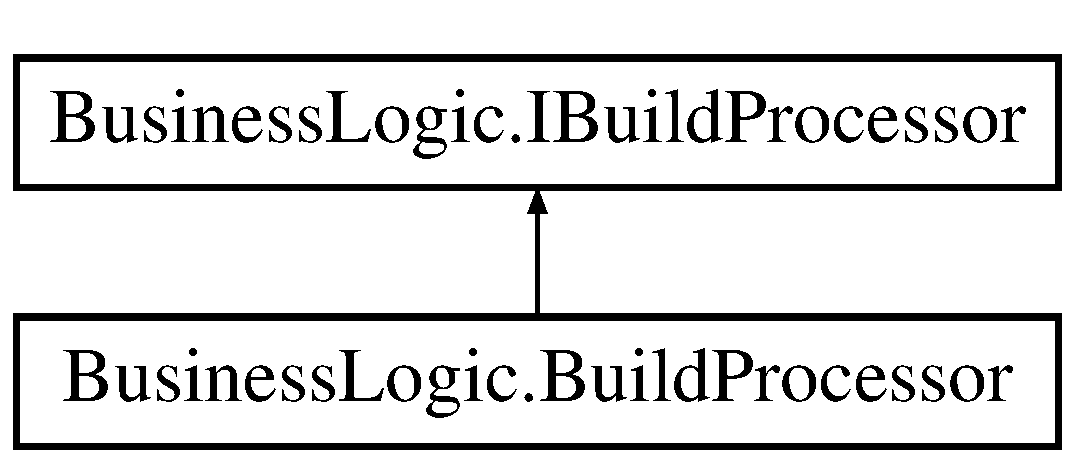
\includegraphics[height=2.000000cm]{class_business_logic_1_1_build_processor}
\end{center}
\end{figure}
\subsection*{Public Member Functions}
\begin{DoxyCompactItemize}
\item 
\hyperlink{class_business_objects_1_1_finalized_build}{Finalized\+Build} \hyperlink{class_business_logic_1_1_build_processor_a7466ec3a31a7752924ca815e1d8bd5fe}{Data\+Builder} (\hyperlink{class_business_objects_1_1_questionnaire_results}{Questionnaire\+Results} qr)
\begin{DoxyCompactList}\small\item\em Public base method that calls needed methods to complete build. \end{DoxyCompactList}\end{DoxyCompactItemize}
\subsection*{Private Member Functions}
\begin{DoxyCompactItemize}
\item 
void \hyperlink{class_business_logic_1_1_build_processor_ad19fb4a3d40031b59c04aa2c9f563ee9}{Final\+Error\+Check} ()
\begin{DoxyCompactList}\small\item\em Validates the build before returning to ensure all components are correct. \end{DoxyCompactList}\item 
void \hyperlink{class_business_logic_1_1_build_processor_a7b2999f8f325a3eac8d7ac3e2467360e}{Final\+Optical} ()
\begin{DoxyCompactList}\small\item\em Selects the final choice for the optical drive. \end{DoxyCompactList}\item 
void \hyperlink{class_business_logic_1_1_build_processor_a736030c17f756a67be21d12063588514}{Contingency\+Builder} (bool major\+Fault, bool needs\+G\+PU, bool needs\+Optical)
\begin{DoxyCompactList}\small\item\em Takes fault results from Final\+Error\+Check and processes for problems. \end{DoxyCompactList}\item 
void \hyperlink{class_business_logic_1_1_build_processor_a48241b1584e37cbfeac0cf69fa573740}{Create\+Finalized\+Build} ()
\begin{DoxyCompactList}\small\item\em Creates the finalized build from all final choice methods. \end{DoxyCompactList}\item 
void \hyperlink{class_business_logic_1_1_build_processor_a6d400fb8ccd35e9f769c8090fc1ad6d9}{C\+P\+U\+Choices\+By\+User\+Needs} (decimal delta)
\begin{DoxyCompactList}\small\item\em Chooses potential C\+P\+Us by user needs. \end{DoxyCompactList}\item 
void \hyperlink{class_business_logic_1_1_build_processor_a4ab80278d65763824f1bfa573738f5f0}{Final\+C\+PU} ()
\begin{DoxyCompactList}\small\item\em Selects the final choice for the C\+PU. \end{DoxyCompactList}\item 
void \hyperlink{class_business_logic_1_1_build_processor_a4d2c79f0219c32564dc53fbbeeb05a73}{G\+P\+U\+Choices\+By\+User\+Needs} (decimal delta)
\begin{DoxyCompactList}\small\item\em Chooses potential G\+P\+Us by user needs. \end{DoxyCompactList}\item 
void \hyperlink{class_business_logic_1_1_build_processor_a2ff04ad18300ae7465005574d0e48772}{Final\+G\+PU} ()
\begin{DoxyCompactList}\small\item\em Selects the final choice for the G\+PU. \end{DoxyCompactList}\item 
void \hyperlink{class_business_logic_1_1_build_processor_a8a8561de9ecd2966034c7a6a69611333}{Motherboard\+Choices\+By\+User\+Needs} (decimal delta)
\begin{DoxyCompactList}\small\item\em Chooses potential motherboards by user needs. \end{DoxyCompactList}\item 
void \hyperlink{class_business_logic_1_1_build_processor_a36b321cf0c93184ab607d7e07993c505}{Final\+Motherboard} ()
\begin{DoxyCompactList}\small\item\em Selects the final choice for the motherboard. \end{DoxyCompactList}\item 
void \hyperlink{class_business_logic_1_1_build_processor_a081f81558d48b97bb26290255aaf57eb}{R\+A\+M\+Choices\+By\+User\+Needs} (decimal delta)
\begin{DoxyCompactList}\small\item\em Chooses portential R\+AM modules by user needs. \end{DoxyCompactList}\item 
void \hyperlink{class_business_logic_1_1_build_processor_a0db9fed50e7a97ad28e59808242126a2}{Final\+R\+AM} ()
\begin{DoxyCompactList}\small\item\em Selects the final choice for the R\+AM \end{DoxyCompactList}\item 
void \hyperlink{class_business_logic_1_1_build_processor_a6548ea5bfcc8e7f9977c7fa7bd5c75a9}{Storage\+Choices\+By\+User\+Needs} (decimal delta)
\begin{DoxyCompactList}\small\item\em Chooses potential storage candidates by user needs. \end{DoxyCompactList}\item 
void \hyperlink{class_business_logic_1_1_build_processor_a9c56c221189ed6bd17ec8ea20593a8c5}{Final\+Storage} ()
\begin{DoxyCompactList}\small\item\em Selects the final choice for the storage. \end{DoxyCompactList}\item 
void \hyperlink{class_business_logic_1_1_build_processor_a202adb3a888d805e5e71e75f67d3f086}{P\+S\+U\+Choices\+By\+User\+Needs} (decimal delta)
\begin{DoxyCompactList}\small\item\em Chooses potential P\+S\+Usby user needs. \end{DoxyCompactList}\item 
void \hyperlink{class_business_logic_1_1_build_processor_aa87a3667f6b2bbc272e864c08ba42364}{Final\+P\+SU} ()
\begin{DoxyCompactList}\small\item\em Selects the final choice for the P\+SU. \end{DoxyCompactList}\item 
void \hyperlink{class_business_logic_1_1_build_processor_a600e948e1baf06c06237742a99a967ff}{Build\+Proportioning} ()
\begin{DoxyCompactList}\small\item\em Creates budget proportions based on standardized build needs. Different use cases require different budget allocations for different parts. \end{DoxyCompactList}\item 
void \hyperlink{class_business_logic_1_1_build_processor_a54da61836d65e0e34a9e2ef76fb1a012}{Create\+All\+Component\+Lists} ()
\begin{DoxyCompactList}\small\item\em Creates all component lists for each component. \end{DoxyCompactList}\end{DoxyCompactItemize}
\subsection*{Private Attributes}
\begin{DoxyCompactItemize}
\item 
\hyperlink{class_business_objects_1_1_questionnaire_results}{Questionnaire\+Results} {\bfseries user\+Needs} = new \hyperlink{class_business_objects_1_1_questionnaire_results}{Questionnaire\+Results}()\hypertarget{class_business_logic_1_1_build_processor_a31e8da8761b5685ab0c25c40019f0764}{}\label{class_business_logic_1_1_build_processor_a31e8da8761b5685ab0c25c40019f0764}

\item 
\hyperlink{class_business_objects_1_1_build_properties}{Build\+Properties} {\bfseries bp} = new \hyperlink{class_business_objects_1_1_build_properties}{Build\+Properties}()\hypertarget{class_business_logic_1_1_build_processor_ab744ddd81ec4a34f0392af4c559eff47}{}\label{class_business_logic_1_1_build_processor_ab744ddd81ec4a34f0392af4c559eff47}

\item 
\hyperlink{class_business_objects_1_1_finalized_build}{Finalized\+Build} {\bfseries fb} = new \hyperlink{class_business_objects_1_1_finalized_build}{Finalized\+Build}()\hypertarget{class_business_logic_1_1_build_processor_a427ec4e6cc78a30ecee4ca94a4427cdb}{}\label{class_business_logic_1_1_build_processor_a427ec4e6cc78a30ecee4ca94a4427cdb}

\item 
const decimal {\bfseries base\+Delta} = 0M\hypertarget{class_business_logic_1_1_build_processor_a7466ca238311159f16e9eb8661fa99bc}{}\label{class_business_logic_1_1_build_processor_a7466ca238311159f16e9eb8661fa99bc}

\item 
decimal {\bfseries budget}\hypertarget{class_business_logic_1_1_build_processor_af1ad16921df1a5ce1eab8c607ba5fca4}{}\label{class_business_logic_1_1_build_processor_af1ad16921df1a5ce1eab8c607ba5fca4}

\item 
string {\bfseries optical\+Type}\hypertarget{class_business_logic_1_1_build_processor_a6af40fa6fc37eccdc6e3286b03c7dcd2}{}\label{class_business_logic_1_1_build_processor_a6af40fa6fc37eccdc6e3286b03c7dcd2}

\item 
List$<$ \hyperlink{class_business_objects_1_1_c_p_u}{C\+PU} $>$ {\bfseries all\+C\+PU}\hypertarget{class_business_logic_1_1_build_processor_adae821c7ea289141aef0a8cf78ad7f40}{}\label{class_business_logic_1_1_build_processor_adae821c7ea289141aef0a8cf78ad7f40}

\item 
List$<$ \hyperlink{class_business_objects_1_1_g_p_u}{G\+PU} $>$ {\bfseries all\+G\+PU}\hypertarget{class_business_logic_1_1_build_processor_a7dfcf48e00c6ea79790e7ce9d7503147}{}\label{class_business_logic_1_1_build_processor_a7dfcf48e00c6ea79790e7ce9d7503147}

\item 
List$<$ \hyperlink{class_business_objects_1_1_motherboard}{Motherboard} $>$ {\bfseries all\+Motherboards}\hypertarget{class_business_logic_1_1_build_processor_a5687ac445787bb6f6cdfc6bf0e39296f}{}\label{class_business_logic_1_1_build_processor_a5687ac445787bb6f6cdfc6bf0e39296f}

\item 
List$<$ \hyperlink{class_business_objects_1_1_r_a_m}{R\+AM} $>$ {\bfseries all\+R\+AM}\hypertarget{class_business_logic_1_1_build_processor_a357ab412eedca92d661b256099170bf9}{}\label{class_business_logic_1_1_build_processor_a357ab412eedca92d661b256099170bf9}

\item 
List$<$ \hyperlink{class_business_objects_1_1_storage}{Storage} $>$ {\bfseries all\+Storage}\hypertarget{class_business_logic_1_1_build_processor_a4b1eaf8478bdaa2a6ce5656286c076d9}{}\label{class_business_logic_1_1_build_processor_a4b1eaf8478bdaa2a6ce5656286c076d9}

\item 
List$<$ \hyperlink{class_business_objects_1_1_p_s_u}{P\+SU} $>$ {\bfseries all\+P\+SU}\hypertarget{class_business_logic_1_1_build_processor_aeb1bcd7c5f31090e401a66ca0a5a8774}{}\label{class_business_logic_1_1_build_processor_aeb1bcd7c5f31090e401a66ca0a5a8774}

\item 
List$<$ \hyperlink{class_business_objects_1_1_optical}{Optical} $>$ {\bfseries optical\+By\+Type}\hypertarget{class_business_logic_1_1_build_processor_a80a6534a685e310877f79f23e6b68225}{}\label{class_business_logic_1_1_build_processor_a80a6534a685e310877f79f23e6b68225}

\item 
List$<$ \hyperlink{class_business_objects_1_1_c_p_u}{C\+PU} $>$ {\bfseries preliminary\+C\+PU} = new List$<$\hyperlink{class_business_objects_1_1_c_p_u}{C\+PU}$>$()\hypertarget{class_business_logic_1_1_build_processor_a1fe14814390cf9a15dc4435b4e1c82b7}{}\label{class_business_logic_1_1_build_processor_a1fe14814390cf9a15dc4435b4e1c82b7}

\item 
List$<$ \hyperlink{class_business_objects_1_1_g_p_u}{G\+PU} $>$ {\bfseries preliminary\+G\+PU} = new List$<$\hyperlink{class_business_objects_1_1_g_p_u}{G\+PU}$>$()\hypertarget{class_business_logic_1_1_build_processor_ac0cc52090eca8883aaf5e4e131132dd8}{}\label{class_business_logic_1_1_build_processor_ac0cc52090eca8883aaf5e4e131132dd8}

\item 
List$<$ \hyperlink{class_business_objects_1_1_motherboard}{Motherboard} $>$ {\bfseries preliminary\+Motherboards} = new List$<$\hyperlink{class_business_objects_1_1_motherboard}{Motherboard}$>$()\hypertarget{class_business_logic_1_1_build_processor_ad32e0709a7660d47c8aaa9610c270efe}{}\label{class_business_logic_1_1_build_processor_ad32e0709a7660d47c8aaa9610c270efe}

\item 
List$<$ \hyperlink{class_business_objects_1_1_r_a_m}{R\+AM} $>$ {\bfseries preliminary\+R\+AM} = new List$<$\hyperlink{class_business_objects_1_1_r_a_m}{R\+AM}$>$()\hypertarget{class_business_logic_1_1_build_processor_a7d306da9a0e14537b644bd1b455e2b4c}{}\label{class_business_logic_1_1_build_processor_a7d306da9a0e14537b644bd1b455e2b4c}

\item 
List$<$ \hyperlink{class_business_objects_1_1_storage}{Storage} $>$ {\bfseries preliminary\+Storage} = new List$<$\hyperlink{class_business_objects_1_1_storage}{Storage}$>$()\hypertarget{class_business_logic_1_1_build_processor_ac1b65e705f9bab09b2bbaffe6aa56b08}{}\label{class_business_logic_1_1_build_processor_ac1b65e705f9bab09b2bbaffe6aa56b08}

\item 
List$<$ \hyperlink{class_business_objects_1_1_p_s_u}{P\+SU} $>$ {\bfseries preliminary\+P\+SU} = new List$<$\hyperlink{class_business_objects_1_1_p_s_u}{P\+SU}$>$()\hypertarget{class_business_logic_1_1_build_processor_a450fd81c9210fe84c16f34ac26d9995c}{}\label{class_business_logic_1_1_build_processor_a450fd81c9210fe84c16f34ac26d9995c}

\item 
\hyperlink{class_business_objects_1_1_c_p_u}{C\+PU} {\bfseries C\+P\+U\+Choice} = new \hyperlink{class_business_objects_1_1_c_p_u}{C\+PU}()\hypertarget{class_business_logic_1_1_build_processor_a2c842d5e2a425dfab029e084857783bb}{}\label{class_business_logic_1_1_build_processor_a2c842d5e2a425dfab029e084857783bb}

\item 
\hyperlink{class_business_objects_1_1_g_p_u}{G\+PU} {\bfseries G\+P\+U\+Choice} = new \hyperlink{class_business_objects_1_1_g_p_u}{G\+PU}()\hypertarget{class_business_logic_1_1_build_processor_abd02f717d13b938b7d615962b35a0fe1}{}\label{class_business_logic_1_1_build_processor_abd02f717d13b938b7d615962b35a0fe1}

\item 
\hyperlink{class_business_objects_1_1_motherboard}{Motherboard} {\bfseries motherboard\+Choice} = new \hyperlink{class_business_objects_1_1_motherboard}{Motherboard}()\hypertarget{class_business_logic_1_1_build_processor_a4d1aaf88ed0a083847f1dd1f9a7c1143}{}\label{class_business_logic_1_1_build_processor_a4d1aaf88ed0a083847f1dd1f9a7c1143}

\item 
\hyperlink{class_business_objects_1_1_r_a_m}{R\+AM} {\bfseries R\+A\+M\+Choice} = new \hyperlink{class_business_objects_1_1_r_a_m}{R\+AM}()\hypertarget{class_business_logic_1_1_build_processor_ab1bfcbae80f18cc7b46906c06d2315eb}{}\label{class_business_logic_1_1_build_processor_ab1bfcbae80f18cc7b46906c06d2315eb}

\item 
\hyperlink{class_business_objects_1_1_r_a_m}{R\+AM} {\bfseries R\+A\+M\+Preliminary} = new \hyperlink{class_business_objects_1_1_r_a_m}{R\+AM}()\hypertarget{class_business_logic_1_1_build_processor_a3c757b2ba0280a37e48a7172078da541}{}\label{class_business_logic_1_1_build_processor_a3c757b2ba0280a37e48a7172078da541}

\item 
\hyperlink{class_business_objects_1_1_storage}{Storage} {\bfseries storage\+Choice} = new \hyperlink{class_business_objects_1_1_storage}{Storage}()\hypertarget{class_business_logic_1_1_build_processor_a787043eb1b824d8ca99f451f90c3b05d}{}\label{class_business_logic_1_1_build_processor_a787043eb1b824d8ca99f451f90c3b05d}

\item 
\hyperlink{class_business_objects_1_1_p_s_u}{P\+SU} {\bfseries P\+S\+U\+Choice} = new \hyperlink{class_business_objects_1_1_p_s_u}{P\+SU}()\hypertarget{class_business_logic_1_1_build_processor_a132211a2121f81b04173466a6ddcbb55}{}\label{class_business_logic_1_1_build_processor_a132211a2121f81b04173466a6ddcbb55}

\item 
\hyperlink{class_business_objects_1_1_optical}{Optical} {\bfseries optical\+Choice} = new \hyperlink{class_business_objects_1_1_optical}{Optical}()\hypertarget{class_business_logic_1_1_build_processor_a9b9203f51653d018460765d3ac578327}{}\label{class_business_logic_1_1_build_processor_a9b9203f51653d018460765d3ac578327}

\end{DoxyCompactItemize}


\subsection{Detailed Description}
Clas tasked with processing of questionnaire data to build a system. 



Definition at line 14 of file Build\+Processor.\+cs.



\subsection{Member Function Documentation}
\index{Business\+Logic\+::\+Build\+Processor@{Business\+Logic\+::\+Build\+Processor}!Build\+Proportioning@{Build\+Proportioning}}
\index{Build\+Proportioning@{Build\+Proportioning}!Business\+Logic\+::\+Build\+Processor@{Business\+Logic\+::\+Build\+Processor}}
\subsubsection[{\texorpdfstring{Build\+Proportioning()}{BuildProportioning()}}]{\setlength{\rightskip}{0pt plus 5cm}void Business\+Logic.\+Build\+Processor.\+Build\+Proportioning (
\begin{DoxyParamCaption}
{}
\end{DoxyParamCaption}
)\hspace{0.3cm}{\ttfamily [private]}}\hypertarget{class_business_logic_1_1_build_processor_a600e948e1baf06c06237742a99a967ff}{}\label{class_business_logic_1_1_build_processor_a600e948e1baf06c06237742a99a967ff}


Creates budget proportions based on standardized build needs. Different use cases require different budget allocations for different parts. 



Definition at line 629 of file Build\+Processor.\+cs.

\index{Business\+Logic\+::\+Build\+Processor@{Business\+Logic\+::\+Build\+Processor}!Contingency\+Builder@{Contingency\+Builder}}
\index{Contingency\+Builder@{Contingency\+Builder}!Business\+Logic\+::\+Build\+Processor@{Business\+Logic\+::\+Build\+Processor}}
\subsubsection[{\texorpdfstring{Contingency\+Builder(bool major\+Fault, bool needs\+G\+P\+U, bool needs\+Optical)}{ContingencyBuilder(bool majorFault, bool needsGPU, bool needsOptical)}}]{\setlength{\rightskip}{0pt plus 5cm}void Business\+Logic.\+Build\+Processor.\+Contingency\+Builder (
\begin{DoxyParamCaption}
\item[{bool}]{major\+Fault, }
\item[{bool}]{needs\+G\+PU, }
\item[{bool}]{needs\+Optical}
\end{DoxyParamCaption}
)\hspace{0.3cm}{\ttfamily [private]}}\hypertarget{class_business_logic_1_1_build_processor_a736030c17f756a67be21d12063588514}{}\label{class_business_logic_1_1_build_processor_a736030c17f756a67be21d12063588514}


Takes fault results from Final\+Error\+Check and processes for problems. 


\begin{DoxyParams}{Parameters}
{\em major\+Fault} & if set to {\ttfamily true}, \mbox{[}major fault\mbox{]}. Represents a significant problem with the build.\\
\hline
{\em needs\+G\+PU} & if set to {\ttfamily true} \mbox{[}needs gpu\mbox{]}. Represents the build does not have a processor capable of on-\/die graphics. A G\+PU must be selected.\\
\hline
{\em needs\+Optical} & if set to {\ttfamily true} \mbox{[}needs optical\mbox{]}. Represents a fault of not being able to pull an applicable optical drive.\\
\hline
\end{DoxyParams}


Definition at line 137 of file Build\+Processor.\+cs.

\index{Business\+Logic\+::\+Build\+Processor@{Business\+Logic\+::\+Build\+Processor}!C\+P\+U\+Choices\+By\+User\+Needs@{C\+P\+U\+Choices\+By\+User\+Needs}}
\index{C\+P\+U\+Choices\+By\+User\+Needs@{C\+P\+U\+Choices\+By\+User\+Needs}!Business\+Logic\+::\+Build\+Processor@{Business\+Logic\+::\+Build\+Processor}}
\subsubsection[{\texorpdfstring{C\+P\+U\+Choices\+By\+User\+Needs(decimal delta)}{CPUChoicesByUserNeeds(decimal delta)}}]{\setlength{\rightskip}{0pt plus 5cm}void Business\+Logic.\+Build\+Processor.\+C\+P\+U\+Choices\+By\+User\+Needs (
\begin{DoxyParamCaption}
\item[{decimal}]{delta}
\end{DoxyParamCaption}
)\hspace{0.3cm}{\ttfamily [private]}}\hypertarget{class_business_logic_1_1_build_processor_a6d400fb8ccd35e9f769c8090fc1ad6d9}{}\label{class_business_logic_1_1_build_processor_a6d400fb8ccd35e9f769c8090fc1ad6d9}


Chooses potential C\+P\+Us by user needs. 


\begin{DoxyParams}{Parameters}
{\em delta} & The price delta. Used for recursion to increasingly expand the price delta.\\
\hline
\end{DoxyParams}


Definition at line 234 of file Build\+Processor.\+cs.

\index{Business\+Logic\+::\+Build\+Processor@{Business\+Logic\+::\+Build\+Processor}!Create\+All\+Component\+Lists@{Create\+All\+Component\+Lists}}
\index{Create\+All\+Component\+Lists@{Create\+All\+Component\+Lists}!Business\+Logic\+::\+Build\+Processor@{Business\+Logic\+::\+Build\+Processor}}
\subsubsection[{\texorpdfstring{Create\+All\+Component\+Lists()}{CreateAllComponentLists()}}]{\setlength{\rightskip}{0pt plus 5cm}void Business\+Logic.\+Build\+Processor.\+Create\+All\+Component\+Lists (
\begin{DoxyParamCaption}
{}
\end{DoxyParamCaption}
)\hspace{0.3cm}{\ttfamily [private]}}\hypertarget{class_business_logic_1_1_build_processor_a54da61836d65e0e34a9e2ef76fb1a012}{}\label{class_business_logic_1_1_build_processor_a54da61836d65e0e34a9e2ef76fb1a012}


Creates all component lists for each component. 

Special attention is needed for the optical type, so the stored procedure can pull the applicable types of ddrives only.

Definition at line 702 of file Build\+Processor.\+cs.

\index{Business\+Logic\+::\+Build\+Processor@{Business\+Logic\+::\+Build\+Processor}!Create\+Finalized\+Build@{Create\+Finalized\+Build}}
\index{Create\+Finalized\+Build@{Create\+Finalized\+Build}!Business\+Logic\+::\+Build\+Processor@{Business\+Logic\+::\+Build\+Processor}}
\subsubsection[{\texorpdfstring{Create\+Finalized\+Build()}{CreateFinalizedBuild()}}]{\setlength{\rightskip}{0pt plus 5cm}void Business\+Logic.\+Build\+Processor.\+Create\+Finalized\+Build (
\begin{DoxyParamCaption}
{}
\end{DoxyParamCaption}
)\hspace{0.3cm}{\ttfamily [private]}}\hypertarget{class_business_logic_1_1_build_processor_a48241b1584e37cbfeac0cf69fa573740}{}\label{class_business_logic_1_1_build_processor_a48241b1584e37cbfeac0cf69fa573740}


Creates the finalized build from all final choice methods. 



Definition at line 219 of file Build\+Processor.\+cs.

\index{Business\+Logic\+::\+Build\+Processor@{Business\+Logic\+::\+Build\+Processor}!Data\+Builder@{Data\+Builder}}
\index{Data\+Builder@{Data\+Builder}!Business\+Logic\+::\+Build\+Processor@{Business\+Logic\+::\+Build\+Processor}}
\subsubsection[{\texorpdfstring{Data\+Builder(\+Questionnaire\+Results qr)}{DataBuilder(QuestionnaireResults qr)}}]{\setlength{\rightskip}{0pt plus 5cm}{\bf Finalized\+Build} Business\+Logic.\+Build\+Processor.\+Data\+Builder (
\begin{DoxyParamCaption}
\item[{{\bf Questionnaire\+Results}}]{qr}
\end{DoxyParamCaption}
)}\hypertarget{class_business_logic_1_1_build_processor_a7466ec3a31a7752924ca815e1d8bd5fe}{}\label{class_business_logic_1_1_build_processor_a7466ec3a31a7752924ca815e1d8bd5fe}


Public base method that calls needed methods to complete build. 


\begin{DoxyParams}{Parameters}
{\em qr} & The questionnaire data.\\
\hline
\end{DoxyParams}
\begin{DoxyReturn}{Returns}
Finalized\+Build with all build components.
\end{DoxyReturn}


Implements \hyperlink{interface_business_logic_1_1_i_build_processor}{Business\+Logic.\+I\+Build\+Processor}.



Definition at line 54 of file Build\+Processor.\+cs.

\index{Business\+Logic\+::\+Build\+Processor@{Business\+Logic\+::\+Build\+Processor}!Final\+C\+PU@{Final\+C\+PU}}
\index{Final\+C\+PU@{Final\+C\+PU}!Business\+Logic\+::\+Build\+Processor@{Business\+Logic\+::\+Build\+Processor}}
\subsubsection[{\texorpdfstring{Final\+C\+P\+U()}{FinalCPU()}}]{\setlength{\rightskip}{0pt plus 5cm}void Business\+Logic.\+Build\+Processor.\+Final\+C\+PU (
\begin{DoxyParamCaption}
{}
\end{DoxyParamCaption}
)\hspace{0.3cm}{\ttfamily [private]}}\hypertarget{class_business_logic_1_1_build_processor_a4ab80278d65763824f1bfa573738f5f0}{}\label{class_business_logic_1_1_build_processor_a4ab80278d65763824f1bfa573738f5f0}


Selects the final choice for the C\+PU. 



Definition at line 253 of file Build\+Processor.\+cs.

\index{Business\+Logic\+::\+Build\+Processor@{Business\+Logic\+::\+Build\+Processor}!Final\+Error\+Check@{Final\+Error\+Check}}
\index{Final\+Error\+Check@{Final\+Error\+Check}!Business\+Logic\+::\+Build\+Processor@{Business\+Logic\+::\+Build\+Processor}}
\subsubsection[{\texorpdfstring{Final\+Error\+Check()}{FinalErrorCheck()}}]{\setlength{\rightskip}{0pt plus 5cm}void Business\+Logic.\+Build\+Processor.\+Final\+Error\+Check (
\begin{DoxyParamCaption}
{}
\end{DoxyParamCaption}
)\hspace{0.3cm}{\ttfamily [private]}}\hypertarget{class_business_logic_1_1_build_processor_ad19fb4a3d40031b59c04aa2c9f563ee9}{}\label{class_business_logic_1_1_build_processor_ad19fb4a3d40031b59c04aa2c9f563ee9}


Validates the build before returning to ensure all components are correct. 

This method calls the Contingency\+Builder and passes the results of the tests. 

Definition at line 88 of file Build\+Processor.\+cs.

\index{Business\+Logic\+::\+Build\+Processor@{Business\+Logic\+::\+Build\+Processor}!Final\+G\+PU@{Final\+G\+PU}}
\index{Final\+G\+PU@{Final\+G\+PU}!Business\+Logic\+::\+Build\+Processor@{Business\+Logic\+::\+Build\+Processor}}
\subsubsection[{\texorpdfstring{Final\+G\+P\+U()}{FinalGPU()}}]{\setlength{\rightskip}{0pt plus 5cm}void Business\+Logic.\+Build\+Processor.\+Final\+G\+PU (
\begin{DoxyParamCaption}
{}
\end{DoxyParamCaption}
)\hspace{0.3cm}{\ttfamily [private]}}\hypertarget{class_business_logic_1_1_build_processor_a2ff04ad18300ae7465005574d0e48772}{}\label{class_business_logic_1_1_build_processor_a2ff04ad18300ae7465005574d0e48772}


Selects the final choice for the G\+PU. 



Definition at line 292 of file Build\+Processor.\+cs.

\index{Business\+Logic\+::\+Build\+Processor@{Business\+Logic\+::\+Build\+Processor}!Final\+Motherboard@{Final\+Motherboard}}
\index{Final\+Motherboard@{Final\+Motherboard}!Business\+Logic\+::\+Build\+Processor@{Business\+Logic\+::\+Build\+Processor}}
\subsubsection[{\texorpdfstring{Final\+Motherboard()}{FinalMotherboard()}}]{\setlength{\rightskip}{0pt plus 5cm}void Business\+Logic.\+Build\+Processor.\+Final\+Motherboard (
\begin{DoxyParamCaption}
{}
\end{DoxyParamCaption}
)\hspace{0.3cm}{\ttfamily [private]}}\hypertarget{class_business_logic_1_1_build_processor_a36b321cf0c93184ab607d7e07993c505}{}\label{class_business_logic_1_1_build_processor_a36b321cf0c93184ab607d7e07993c505}


Selects the final choice for the motherboard. 



Definition at line 340 of file Build\+Processor.\+cs.

\index{Business\+Logic\+::\+Build\+Processor@{Business\+Logic\+::\+Build\+Processor}!Final\+Optical@{Final\+Optical}}
\index{Final\+Optical@{Final\+Optical}!Business\+Logic\+::\+Build\+Processor@{Business\+Logic\+::\+Build\+Processor}}
\subsubsection[{\texorpdfstring{Final\+Optical()}{FinalOptical()}}]{\setlength{\rightskip}{0pt plus 5cm}void Business\+Logic.\+Build\+Processor.\+Final\+Optical (
\begin{DoxyParamCaption}
{}
\end{DoxyParamCaption}
)\hspace{0.3cm}{\ttfamily [private]}}\hypertarget{class_business_logic_1_1_build_processor_a7b2999f8f325a3eac8d7ac3e2467360e}{}\label{class_business_logic_1_1_build_processor_a7b2999f8f325a3eac8d7ac3e2467360e}


Selects the final choice for the optical drive. 



Definition at line 116 of file Build\+Processor.\+cs.

\index{Business\+Logic\+::\+Build\+Processor@{Business\+Logic\+::\+Build\+Processor}!Final\+P\+SU@{Final\+P\+SU}}
\index{Final\+P\+SU@{Final\+P\+SU}!Business\+Logic\+::\+Build\+Processor@{Business\+Logic\+::\+Build\+Processor}}
\subsubsection[{\texorpdfstring{Final\+P\+S\+U()}{FinalPSU()}}]{\setlength{\rightskip}{0pt plus 5cm}void Business\+Logic.\+Build\+Processor.\+Final\+P\+SU (
\begin{DoxyParamCaption}
{}
\end{DoxyParamCaption}
)\hspace{0.3cm}{\ttfamily [private]}}\hypertarget{class_business_logic_1_1_build_processor_aa87a3667f6b2bbc272e864c08ba42364}{}\label{class_business_logic_1_1_build_processor_aa87a3667f6b2bbc272e864c08ba42364}


Selects the final choice for the P\+SU. 



Definition at line 613 of file Build\+Processor.\+cs.

\index{Business\+Logic\+::\+Build\+Processor@{Business\+Logic\+::\+Build\+Processor}!Final\+R\+AM@{Final\+R\+AM}}
\index{Final\+R\+AM@{Final\+R\+AM}!Business\+Logic\+::\+Build\+Processor@{Business\+Logic\+::\+Build\+Processor}}
\subsubsection[{\texorpdfstring{Final\+R\+A\+M()}{FinalRAM()}}]{\setlength{\rightskip}{0pt plus 5cm}void Business\+Logic.\+Build\+Processor.\+Final\+R\+AM (
\begin{DoxyParamCaption}
{}
\end{DoxyParamCaption}
)\hspace{0.3cm}{\ttfamily [private]}}\hypertarget{class_business_logic_1_1_build_processor_a0db9fed50e7a97ad28e59808242126a2}{}\label{class_business_logic_1_1_build_processor_a0db9fed50e7a97ad28e59808242126a2}


Selects the final choice for the R\+AM 



Definition at line 453 of file Build\+Processor.\+cs.

\index{Business\+Logic\+::\+Build\+Processor@{Business\+Logic\+::\+Build\+Processor}!Final\+Storage@{Final\+Storage}}
\index{Final\+Storage@{Final\+Storage}!Business\+Logic\+::\+Build\+Processor@{Business\+Logic\+::\+Build\+Processor}}
\subsubsection[{\texorpdfstring{Final\+Storage()}{FinalStorage()}}]{\setlength{\rightskip}{0pt plus 5cm}void Business\+Logic.\+Build\+Processor.\+Final\+Storage (
\begin{DoxyParamCaption}
{}
\end{DoxyParamCaption}
)\hspace{0.3cm}{\ttfamily [private]}}\hypertarget{class_business_logic_1_1_build_processor_a9c56c221189ed6bd17ec8ea20593a8c5}{}\label{class_business_logic_1_1_build_processor_a9c56c221189ed6bd17ec8ea20593a8c5}


Selects the final choice for the storage. 

This method takes into account the use case for the user. If the user needs high performance, an S\+SD is selected. 

Definition at line 539 of file Build\+Processor.\+cs.

\index{Business\+Logic\+::\+Build\+Processor@{Business\+Logic\+::\+Build\+Processor}!G\+P\+U\+Choices\+By\+User\+Needs@{G\+P\+U\+Choices\+By\+User\+Needs}}
\index{G\+P\+U\+Choices\+By\+User\+Needs@{G\+P\+U\+Choices\+By\+User\+Needs}!Business\+Logic\+::\+Build\+Processor@{Business\+Logic\+::\+Build\+Processor}}
\subsubsection[{\texorpdfstring{G\+P\+U\+Choices\+By\+User\+Needs(decimal delta)}{GPUChoicesByUserNeeds(decimal delta)}}]{\setlength{\rightskip}{0pt plus 5cm}void Business\+Logic.\+Build\+Processor.\+G\+P\+U\+Choices\+By\+User\+Needs (
\begin{DoxyParamCaption}
\item[{decimal}]{delta}
\end{DoxyParamCaption}
)\hspace{0.3cm}{\ttfamily [private]}}\hypertarget{class_business_logic_1_1_build_processor_a4d2c79f0219c32564dc53fbbeeb05a73}{}\label{class_business_logic_1_1_build_processor_a4d2c79f0219c32564dc53fbbeeb05a73}


Chooses potential G\+P\+Us by user needs. 


\begin{DoxyParams}{Parameters}
{\em delta} & The price delta. Used for recursion to increasingly expand the price delta.\\
\hline
\end{DoxyParams}


Definition at line 270 of file Build\+Processor.\+cs.

\index{Business\+Logic\+::\+Build\+Processor@{Business\+Logic\+::\+Build\+Processor}!Motherboard\+Choices\+By\+User\+Needs@{Motherboard\+Choices\+By\+User\+Needs}}
\index{Motherboard\+Choices\+By\+User\+Needs@{Motherboard\+Choices\+By\+User\+Needs}!Business\+Logic\+::\+Build\+Processor@{Business\+Logic\+::\+Build\+Processor}}
\subsubsection[{\texorpdfstring{Motherboard\+Choices\+By\+User\+Needs(decimal delta)}{MotherboardChoicesByUserNeeds(decimal delta)}}]{\setlength{\rightskip}{0pt plus 5cm}void Business\+Logic.\+Build\+Processor.\+Motherboard\+Choices\+By\+User\+Needs (
\begin{DoxyParamCaption}
\item[{decimal}]{delta}
\end{DoxyParamCaption}
)\hspace{0.3cm}{\ttfamily [private]}}\hypertarget{class_business_logic_1_1_build_processor_a8a8561de9ecd2966034c7a6a69611333}{}\label{class_business_logic_1_1_build_processor_a8a8561de9ecd2966034c7a6a69611333}


Chooses potential motherboards by user needs. 

This must be called after the Final\+C\+PU method. Not doing so will cause incompatibilities between the C\+PU and motherboard. 


\begin{DoxyParams}{Parameters}
{\em delta} & The price delta. Used for recursion to increasingly expand the price delta.\\
\hline
\end{DoxyParams}


Definition at line 315 of file Build\+Processor.\+cs.

\index{Business\+Logic\+::\+Build\+Processor@{Business\+Logic\+::\+Build\+Processor}!P\+S\+U\+Choices\+By\+User\+Needs@{P\+S\+U\+Choices\+By\+User\+Needs}}
\index{P\+S\+U\+Choices\+By\+User\+Needs@{P\+S\+U\+Choices\+By\+User\+Needs}!Business\+Logic\+::\+Build\+Processor@{Business\+Logic\+::\+Build\+Processor}}
\subsubsection[{\texorpdfstring{P\+S\+U\+Choices\+By\+User\+Needs(decimal delta)}{PSUChoicesByUserNeeds(decimal delta)}}]{\setlength{\rightskip}{0pt plus 5cm}void Business\+Logic.\+Build\+Processor.\+P\+S\+U\+Choices\+By\+User\+Needs (
\begin{DoxyParamCaption}
\item[{decimal}]{delta}
\end{DoxyParamCaption}
)\hspace{0.3cm}{\ttfamily [private]}}\hypertarget{class_business_logic_1_1_build_processor_a202adb3a888d805e5e71e75f67d3f086}{}\label{class_business_logic_1_1_build_processor_a202adb3a888d805e5e71e75f67d3f086}


Chooses potential P\+S\+Usby user needs. 

This method must be done last in the build process. Not doing so can result in an inadequate power supply being selected. 


\begin{DoxyParams}{Parameters}
{\em delta} & The price delta. Used for recursion to increasingly expand the price delta.\\
\hline
\end{DoxyParams}


Definition at line 588 of file Build\+Processor.\+cs.

\index{Business\+Logic\+::\+Build\+Processor@{Business\+Logic\+::\+Build\+Processor}!R\+A\+M\+Choices\+By\+User\+Needs@{R\+A\+M\+Choices\+By\+User\+Needs}}
\index{R\+A\+M\+Choices\+By\+User\+Needs@{R\+A\+M\+Choices\+By\+User\+Needs}!Business\+Logic\+::\+Build\+Processor@{Business\+Logic\+::\+Build\+Processor}}
\subsubsection[{\texorpdfstring{R\+A\+M\+Choices\+By\+User\+Needs(decimal delta)}{RAMChoicesByUserNeeds(decimal delta)}}]{\setlength{\rightskip}{0pt plus 5cm}void Business\+Logic.\+Build\+Processor.\+R\+A\+M\+Choices\+By\+User\+Needs (
\begin{DoxyParamCaption}
\item[{decimal}]{delta}
\end{DoxyParamCaption}
)\hspace{0.3cm}{\ttfamily [private]}}\hypertarget{class_business_logic_1_1_build_processor_a081f81558d48b97bb26290255aaf57eb}{}\label{class_business_logic_1_1_build_processor_a081f81558d48b97bb26290255aaf57eb}


Chooses portential R\+AM modules by user needs. 

This must be called after the Final\+Motherboard method. Not doing so will cause incompatibilities bwtween the motherboard and R\+AM. 


\begin{DoxyParams}{Parameters}
{\em delta} & The price delta. Used for recursion to increasingly expand the price delta.\\
\hline
\end{DoxyParams}


Definition at line 387 of file Build\+Processor.\+cs.

\index{Business\+Logic\+::\+Build\+Processor@{Business\+Logic\+::\+Build\+Processor}!Storage\+Choices\+By\+User\+Needs@{Storage\+Choices\+By\+User\+Needs}}
\index{Storage\+Choices\+By\+User\+Needs@{Storage\+Choices\+By\+User\+Needs}!Business\+Logic\+::\+Build\+Processor@{Business\+Logic\+::\+Build\+Processor}}
\subsubsection[{\texorpdfstring{Storage\+Choices\+By\+User\+Needs(decimal delta)}{StorageChoicesByUserNeeds(decimal delta)}}]{\setlength{\rightskip}{0pt plus 5cm}void Business\+Logic.\+Build\+Processor.\+Storage\+Choices\+By\+User\+Needs (
\begin{DoxyParamCaption}
\item[{decimal}]{delta}
\end{DoxyParamCaption}
)\hspace{0.3cm}{\ttfamily [private]}}\hypertarget{class_business_logic_1_1_build_processor_a6548ea5bfcc8e7f9977c7fa7bd5c75a9}{}\label{class_business_logic_1_1_build_processor_a6548ea5bfcc8e7f9977c7fa7bd5c75a9}


Chooses potential storage candidates by user needs. 

The method differentiates between H\+DD and S\+SD based on the user\textquotesingle{}s needs. 


\begin{DoxyParams}{Parameters}
{\em delta} & The price delta. Used for recursion to increasingly expand the price delta.\\
\hline
\end{DoxyParams}


Definition at line 489 of file Build\+Processor.\+cs.



The documentation for this class was generated from the following file\+:\begin{DoxyCompactItemize}
\item 
C\+:/\+Users/nh228u08/\+Desktop/\+Final\+Project/\+Final\+Project/\+P\+C\+Builder/\+Business\+Logic/Build\+Processor.\+cs\end{DoxyCompactItemize}

\hypertarget{class_business_objects_1_1_build_properties}{}\section{Business\+Objects.\+Build\+Properties Class Reference}
\label{class_business_objects_1_1_build_properties}\index{Business\+Objects.\+Build\+Properties@{Business\+Objects.\+Build\+Properties}}


\hyperlink{class_business_objects_1_1_build_properties}{Build\+Properties} object to hold necessary data on the budget of the build.  


\subsection*{Properties}
\begin{DoxyCompactItemize}
\item 
decimal {\bfseries C\+P\+U\+Budget}\hspace{0.3cm}{\ttfamily  \mbox{[}get, set\mbox{]}}\hypertarget{class_business_objects_1_1_build_properties_ad47af7204e41617b511c28fe51bb2768}{}\label{class_business_objects_1_1_build_properties_ad47af7204e41617b511c28fe51bb2768}

\item 
decimal {\bfseries G\+P\+U\+Budget}\hspace{0.3cm}{\ttfamily  \mbox{[}get, set\mbox{]}}\hypertarget{class_business_objects_1_1_build_properties_ae0f7d3ad79d4d78b73dba502a0f82147}{}\label{class_business_objects_1_1_build_properties_ae0f7d3ad79d4d78b73dba502a0f82147}

\item 
decimal {\bfseries Motherboard\+Budget}\hspace{0.3cm}{\ttfamily  \mbox{[}get, set\mbox{]}}\hypertarget{class_business_objects_1_1_build_properties_a38e2be70d3a2a5cddb453c94132dbeaf}{}\label{class_business_objects_1_1_build_properties_a38e2be70d3a2a5cddb453c94132dbeaf}

\item 
decimal {\bfseries Optical\+Budget}\hspace{0.3cm}{\ttfamily  \mbox{[}get, set\mbox{]}}\hypertarget{class_business_objects_1_1_build_properties_a69dd67f21573074f826cafc40ecc5bb6}{}\label{class_business_objects_1_1_build_properties_a69dd67f21573074f826cafc40ecc5bb6}

\item 
decimal {\bfseries P\+S\+U\+Budget}\hspace{0.3cm}{\ttfamily  \mbox{[}get, set\mbox{]}}\hypertarget{class_business_objects_1_1_build_properties_abe6c1bb5085fe3d404fadfe9ab48b5fe}{}\label{class_business_objects_1_1_build_properties_abe6c1bb5085fe3d404fadfe9ab48b5fe}

\item 
decimal {\bfseries R\+A\+M\+Budget}\hspace{0.3cm}{\ttfamily  \mbox{[}get, set\mbox{]}}\hypertarget{class_business_objects_1_1_build_properties_a43c5545428656e0f07cd3fa6674abace}{}\label{class_business_objects_1_1_build_properties_a43c5545428656e0f07cd3fa6674abace}

\item 
decimal {\bfseries Storage\+Budget}\hspace{0.3cm}{\ttfamily  \mbox{[}get, set\mbox{]}}\hypertarget{class_business_objects_1_1_build_properties_a4c0a340000beda0f71bb35bf7ba7ee3a}{}\label{class_business_objects_1_1_build_properties_a4c0a340000beda0f71bb35bf7ba7ee3a}

\end{DoxyCompactItemize}


\subsection{Detailed Description}
\hyperlink{class_business_objects_1_1_build_properties}{Build\+Properties} object to hold necessary data on the budget of the build. 



Definition at line 12 of file Build\+Properties.\+cs.



The documentation for this class was generated from the following file\+:\begin{DoxyCompactItemize}
\item 
C\+:/\+Users/nh228u08/\+Desktop/\+Final\+Project/\+Final\+Project/\+P\+C\+Builder/\+Business\+Objects/Build\+Properties.\+cs\end{DoxyCompactItemize}

\hypertarget{class_p_c_builder_forms_1_1_build_results}{}\section{P\+C\+Builder\+Forms.\+Build\+Results Class Reference}
\label{class_p_c_builder_forms_1_1_build_results}\index{P\+C\+Builder\+Forms.\+Build\+Results@{P\+C\+Builder\+Forms.\+Build\+Results}}


\hyperlink{class_p_c_builder_forms_1_1_build_results}{Build\+Results}  


Inheritance diagram for P\+C\+Builder\+Forms.\+Build\+Results\+:\begin{figure}[H]
\begin{center}
\leavevmode
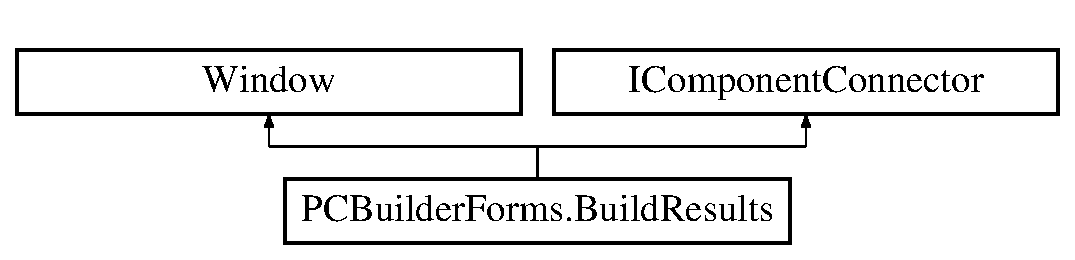
\includegraphics[height=2.000000cm]{class_p_c_builder_forms_1_1_build_results}
\end{center}
\end{figure}
\subsection*{Public Member Functions}
\begin{DoxyCompactItemize}
\item 
void \hyperlink{class_p_c_builder_forms_1_1_build_results_a9c575c605cc69bafccc43687729b9f4c}{Initialize\+Component} ()
\begin{DoxyCompactList}\small\item\em Initialize\+Component \end{DoxyCompactList}\end{DoxyCompactItemize}
\subsection*{Package Attributes}
\begin{DoxyCompactItemize}
\item 
System.\+Windows.\+Controls.\+Label {\bfseries lbl\+C\+P\+U\+Brand}\hypertarget{class_p_c_builder_forms_1_1_build_results_aac326fdead6162a7b42085fce0855dca}{}\label{class_p_c_builder_forms_1_1_build_results_aac326fdead6162a7b42085fce0855dca}

\item 
System.\+Windows.\+Controls.\+Label {\bfseries lbl\+G\+P\+U\+Brand}\hypertarget{class_p_c_builder_forms_1_1_build_results_a98f314ca3e9d7396e4247b9b0992beed}{}\label{class_p_c_builder_forms_1_1_build_results_a98f314ca3e9d7396e4247b9b0992beed}

\item 
System.\+Windows.\+Controls.\+Label {\bfseries lbl\+Motherboard\+Brand}\hypertarget{class_p_c_builder_forms_1_1_build_results_ac72a764b2e7f4c92022e8deff175c37c}{}\label{class_p_c_builder_forms_1_1_build_results_ac72a764b2e7f4c92022e8deff175c37c}

\item 
System.\+Windows.\+Controls.\+Label {\bfseries lbl\+Optical\+Brand}\hypertarget{class_p_c_builder_forms_1_1_build_results_ad051e33b794526b15eb9e8148fd304e2}{}\label{class_p_c_builder_forms_1_1_build_results_ad051e33b794526b15eb9e8148fd304e2}

\item 
System.\+Windows.\+Controls.\+Label {\bfseries lbl\+P\+S\+U\+Brand}\hypertarget{class_p_c_builder_forms_1_1_build_results_a8f2c31ef49d8983133ecbbe2d4bcec94}{}\label{class_p_c_builder_forms_1_1_build_results_a8f2c31ef49d8983133ecbbe2d4bcec94}

\item 
System.\+Windows.\+Controls.\+Label {\bfseries lbl\+R\+A\+M\+Brand}\hypertarget{class_p_c_builder_forms_1_1_build_results_aaa15b511e7a706d64cdb28dde00acd8b}{}\label{class_p_c_builder_forms_1_1_build_results_aaa15b511e7a706d64cdb28dde00acd8b}

\item 
System.\+Windows.\+Controls.\+Label {\bfseries lbl\+Storage\+Brand}\hypertarget{class_p_c_builder_forms_1_1_build_results_a8b34235bb45508dd73516279087aa88f}{}\label{class_p_c_builder_forms_1_1_build_results_a8b34235bb45508dd73516279087aa88f}

\item 
System.\+Windows.\+Controls.\+Label {\bfseries lbl\+C\+P\+U\+Model}\hypertarget{class_p_c_builder_forms_1_1_build_results_a829dc7edfb9410bceb2003ca2f6c552d}{}\label{class_p_c_builder_forms_1_1_build_results_a829dc7edfb9410bceb2003ca2f6c552d}

\item 
System.\+Windows.\+Controls.\+Label {\bfseries lbl\+G\+P\+U\+Model}\hypertarget{class_p_c_builder_forms_1_1_build_results_aca769298463bda8d6ad6ba5dfbd7293d}{}\label{class_p_c_builder_forms_1_1_build_results_aca769298463bda8d6ad6ba5dfbd7293d}

\item 
System.\+Windows.\+Controls.\+Label {\bfseries lbl\+Motherboard\+Model}\hypertarget{class_p_c_builder_forms_1_1_build_results_a24909913f3637a42e848ac097b23fc6b}{}\label{class_p_c_builder_forms_1_1_build_results_a24909913f3637a42e848ac097b23fc6b}

\item 
System.\+Windows.\+Controls.\+Label {\bfseries lbl\+Optical\+Model}\hypertarget{class_p_c_builder_forms_1_1_build_results_a8afd1c8e9fb45844c682abd043f0833a}{}\label{class_p_c_builder_forms_1_1_build_results_a8afd1c8e9fb45844c682abd043f0833a}

\item 
System.\+Windows.\+Controls.\+Label {\bfseries lbl\+P\+S\+U\+Model}\hypertarget{class_p_c_builder_forms_1_1_build_results_a381584a4d0733588caa483bb0c405c68}{}\label{class_p_c_builder_forms_1_1_build_results_a381584a4d0733588caa483bb0c405c68}

\item 
System.\+Windows.\+Controls.\+Label {\bfseries lbl\+R\+A\+M\+Model}\hypertarget{class_p_c_builder_forms_1_1_build_results_a1e9d17258116e11c5648dfcf6e380db5}{}\label{class_p_c_builder_forms_1_1_build_results_a1e9d17258116e11c5648dfcf6e380db5}

\item 
System.\+Windows.\+Controls.\+Label {\bfseries lbl\+Storage\+Model}\hypertarget{class_p_c_builder_forms_1_1_build_results_a5ea5f98a06ca09c3111688c73a466655}{}\label{class_p_c_builder_forms_1_1_build_results_a5ea5f98a06ca09c3111688c73a466655}

\item 
System.\+Windows.\+Controls.\+Label {\bfseries lbl\+C\+P\+U\+Price}\hypertarget{class_p_c_builder_forms_1_1_build_results_abc1a726f02940e6fbe7f987cdb4849ed}{}\label{class_p_c_builder_forms_1_1_build_results_abc1a726f02940e6fbe7f987cdb4849ed}

\item 
System.\+Windows.\+Controls.\+Label {\bfseries lbl\+G\+P\+U\+Price}\hypertarget{class_p_c_builder_forms_1_1_build_results_a4ab79e1bce7d641c083586df73c9308e}{}\label{class_p_c_builder_forms_1_1_build_results_a4ab79e1bce7d641c083586df73c9308e}

\item 
System.\+Windows.\+Controls.\+Label {\bfseries lbl\+Motherboard\+Price}\hypertarget{class_p_c_builder_forms_1_1_build_results_af60eb9523153380fa10597706607b2cd}{}\label{class_p_c_builder_forms_1_1_build_results_af60eb9523153380fa10597706607b2cd}

\item 
System.\+Windows.\+Controls.\+Label {\bfseries lbl\+Optical\+Price}\hypertarget{class_p_c_builder_forms_1_1_build_results_ac4064daf48187fd8db6b9b6edf71a59a}{}\label{class_p_c_builder_forms_1_1_build_results_ac4064daf48187fd8db6b9b6edf71a59a}

\item 
System.\+Windows.\+Controls.\+Label {\bfseries lbl\+P\+S\+U\+Price}\hypertarget{class_p_c_builder_forms_1_1_build_results_af725e7c751a522182b6c906ad340b025}{}\label{class_p_c_builder_forms_1_1_build_results_af725e7c751a522182b6c906ad340b025}

\item 
System.\+Windows.\+Controls.\+Label {\bfseries lbl\+R\+A\+M\+Price}\hypertarget{class_p_c_builder_forms_1_1_build_results_adc5adb7b6e219ff35fbdc944607c695b}{}\label{class_p_c_builder_forms_1_1_build_results_adc5adb7b6e219ff35fbdc944607c695b}

\item 
System.\+Windows.\+Controls.\+Label {\bfseries lbl\+Storage\+Price}\hypertarget{class_p_c_builder_forms_1_1_build_results_a26ae7c8a56885b91872ee41e86829b12}{}\label{class_p_c_builder_forms_1_1_build_results_a26ae7c8a56885b91872ee41e86829b12}

\item 
System.\+Windows.\+Controls.\+Label {\bfseries lbl\+Total\+Price}\hypertarget{class_p_c_builder_forms_1_1_build_results_a357080103fc5b8fcadb2929339225e37}{}\label{class_p_c_builder_forms_1_1_build_results_a357080103fc5b8fcadb2929339225e37}

\end{DoxyCompactItemize}
\subsection*{Private Member Functions}
\begin{DoxyCompactItemize}
\item 
void System.\+Windows.\+Markup.\+I\+Component\+Connector. {\bfseries Connect} (int connection\+Id, object target)\hypertarget{class_p_c_builder_forms_1_1_build_results_a6fa0ebd3e7f1d83778bdf6176cd88013}{}\label{class_p_c_builder_forms_1_1_build_results_a6fa0ebd3e7f1d83778bdf6176cd88013}

\end{DoxyCompactItemize}
\subsection*{Private Attributes}
\begin{DoxyCompactItemize}
\item 
bool {\bfseries \+\_\+content\+Loaded}\hypertarget{class_p_c_builder_forms_1_1_build_results_abee62c73c339faca4908e3ce6dcc0b9f}{}\label{class_p_c_builder_forms_1_1_build_results_abee62c73c339faca4908e3ce6dcc0b9f}

\end{DoxyCompactItemize}


\subsection{Detailed Description}
\hyperlink{class_p_c_builder_forms_1_1_build_results}{Build\+Results} 



Definition at line 41 of file Build\+Results.\+g.\+i.\+cs.



\subsection{Member Function Documentation}
\index{P\+C\+Builder\+Forms\+::\+Build\+Results@{P\+C\+Builder\+Forms\+::\+Build\+Results}!Initialize\+Component@{Initialize\+Component}}
\index{Initialize\+Component@{Initialize\+Component}!P\+C\+Builder\+Forms\+::\+Build\+Results@{P\+C\+Builder\+Forms\+::\+Build\+Results}}
\subsubsection[{\texorpdfstring{Initialize\+Component()}{InitializeComponent()}}]{\setlength{\rightskip}{0pt plus 5cm}void P\+C\+Builder\+Forms.\+Build\+Results.\+Initialize\+Component (
\begin{DoxyParamCaption}
{}
\end{DoxyParamCaption}
)}\hypertarget{class_p_c_builder_forms_1_1_build_results_a9c575c605cc69bafccc43687729b9f4c}{}\label{class_p_c_builder_forms_1_1_build_results_a9c575c605cc69bafccc43687729b9f4c}


Initialize\+Component 



Definition at line 226 of file Build\+Results.\+g.\+i.\+cs.



The documentation for this class was generated from the following file\+:\begin{DoxyCompactItemize}
\item 
C\+:/\+Users/nh228u08/\+Desktop/\+Final\+Project/\+Final\+Project/\+P\+C\+Builder/\+P\+C\+Builder\+Forms/obj/\+Debug/Build\+Results.\+g.\+i.\+cs\end{DoxyCompactItemize}

\hypertarget{class_p_c_builder_m_v_c_1_1_bundle_config}{}\section{P\+C\+Builder\+M\+V\+C.\+Bundle\+Config Class Reference}
\label{class_p_c_builder_m_v_c_1_1_bundle_config}\index{P\+C\+Builder\+M\+V\+C.\+Bundle\+Config@{P\+C\+Builder\+M\+V\+C.\+Bundle\+Config}}


Bundle registration class.  


\subsection*{Static Public Member Functions}
\begin{DoxyCompactItemize}
\item 
static void \hyperlink{class_p_c_builder_m_v_c_1_1_bundle_config_a857c57658698af214b4bbd5e3fc31d78}{Register\+Bundles} (Bundle\+Collection bundles)
\begin{DoxyCompactList}\small\item\em Registers the bundles. \end{DoxyCompactList}\end{DoxyCompactItemize}


\subsection{Detailed Description}
Bundle registration class. 



Definition at line 9 of file Bundle\+Config.\+cs.



\subsection{Member Function Documentation}
\index{P\+C\+Builder\+M\+V\+C\+::\+Bundle\+Config@{P\+C\+Builder\+M\+V\+C\+::\+Bundle\+Config}!Register\+Bundles@{Register\+Bundles}}
\index{Register\+Bundles@{Register\+Bundles}!P\+C\+Builder\+M\+V\+C\+::\+Bundle\+Config@{P\+C\+Builder\+M\+V\+C\+::\+Bundle\+Config}}
\subsubsection[{\texorpdfstring{Register\+Bundles(\+Bundle\+Collection bundles)}{RegisterBundles(BundleCollection bundles)}}]{\setlength{\rightskip}{0pt plus 5cm}static void P\+C\+Builder\+M\+V\+C.\+Bundle\+Config.\+Register\+Bundles (
\begin{DoxyParamCaption}
\item[{Bundle\+Collection}]{bundles}
\end{DoxyParamCaption}
)\hspace{0.3cm}{\ttfamily [static]}}\hypertarget{class_p_c_builder_m_v_c_1_1_bundle_config_a857c57658698af214b4bbd5e3fc31d78}{}\label{class_p_c_builder_m_v_c_1_1_bundle_config_a857c57658698af214b4bbd5e3fc31d78}


Registers the bundles. 


\begin{DoxyParams}{Parameters}
{\em bundles} & The bundles.\\
\hline
\end{DoxyParams}


Definition at line 16 of file Bundle\+Config.\+cs.



The documentation for this class was generated from the following file\+:\begin{DoxyCompactItemize}
\item 
C\+:/\+Users/nh228u08/\+Desktop/\+Final\+Project/\+Final\+Project/\+P\+C\+Builder/\+P\+C\+Builder\+M\+V\+C/\+App\+\_\+\+Start/Bundle\+Config.\+cs\end{DoxyCompactItemize}

\hypertarget{class_p_c_builder_m_v_c_1_1_controllers_1_1_account_controller_1_1_challenge_result}{}\section{P\+C\+Builder\+M\+V\+C.\+Controllers.\+Account\+Controller.\+Challenge\+Result Class Reference}
\label{class_p_c_builder_m_v_c_1_1_controllers_1_1_account_controller_1_1_challenge_result}\index{P\+C\+Builder\+M\+V\+C.\+Controllers.\+Account\+Controller.\+Challenge\+Result@{P\+C\+Builder\+M\+V\+C.\+Controllers.\+Account\+Controller.\+Challenge\+Result}}
Inheritance diagram for P\+C\+Builder\+M\+V\+C.\+Controllers.\+Account\+Controller.\+Challenge\+Result\+:\begin{figure}[H]
\begin{center}
\leavevmode
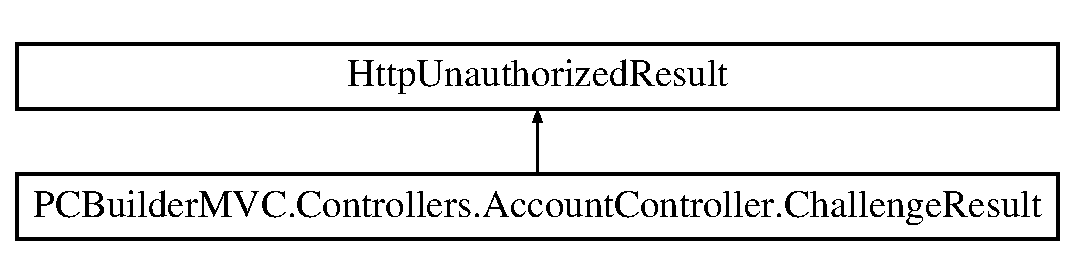
\includegraphics[height=2.000000cm]{class_p_c_builder_m_v_c_1_1_controllers_1_1_account_controller_1_1_challenge_result}
\end{center}
\end{figure}
\subsection*{Public Member Functions}
\begin{DoxyCompactItemize}
\item 
{\bfseries Challenge\+Result} (string provider, string redirect\+Uri)\hypertarget{class_p_c_builder_m_v_c_1_1_controllers_1_1_account_controller_1_1_challenge_result_a78cfcbf7db59c5e894ee96c209afc93c}{}\label{class_p_c_builder_m_v_c_1_1_controllers_1_1_account_controller_1_1_challenge_result_a78cfcbf7db59c5e894ee96c209afc93c}

\item 
{\bfseries Challenge\+Result} (string provider, string redirect\+Uri, string user\+Id)\hypertarget{class_p_c_builder_m_v_c_1_1_controllers_1_1_account_controller_1_1_challenge_result_a2a6e6c2056b0b9ace59f8cc2e0357a64}{}\label{class_p_c_builder_m_v_c_1_1_controllers_1_1_account_controller_1_1_challenge_result_a2a6e6c2056b0b9ace59f8cc2e0357a64}

\item 
override void {\bfseries Execute\+Result} (Controller\+Context context)\hypertarget{class_p_c_builder_m_v_c_1_1_controllers_1_1_account_controller_1_1_challenge_result_ab13dcc9d19f257e306f78f7e96e3fcd1}{}\label{class_p_c_builder_m_v_c_1_1_controllers_1_1_account_controller_1_1_challenge_result_ab13dcc9d19f257e306f78f7e96e3fcd1}

\end{DoxyCompactItemize}
\subsection*{Properties}
\begin{DoxyCompactItemize}
\item 
string {\bfseries Login\+Provider}\hspace{0.3cm}{\ttfamily  \mbox{[}get, set\mbox{]}}\hypertarget{class_p_c_builder_m_v_c_1_1_controllers_1_1_account_controller_1_1_challenge_result_ac7cac910c22fc1c95c7a5a15f575cd5e}{}\label{class_p_c_builder_m_v_c_1_1_controllers_1_1_account_controller_1_1_challenge_result_ac7cac910c22fc1c95c7a5a15f575cd5e}

\item 
string {\bfseries Redirect\+Uri}\hspace{0.3cm}{\ttfamily  \mbox{[}get, set\mbox{]}}\hypertarget{class_p_c_builder_m_v_c_1_1_controllers_1_1_account_controller_1_1_challenge_result_ac4ddc0bc44bfccf0a772e482d9499826}{}\label{class_p_c_builder_m_v_c_1_1_controllers_1_1_account_controller_1_1_challenge_result_ac4ddc0bc44bfccf0a772e482d9499826}

\item 
string {\bfseries User\+Id}\hspace{0.3cm}{\ttfamily  \mbox{[}get, set\mbox{]}}\hypertarget{class_p_c_builder_m_v_c_1_1_controllers_1_1_account_controller_1_1_challenge_result_ab685e3369f605b4bb9b92cc3cd7bb68e}{}\label{class_p_c_builder_m_v_c_1_1_controllers_1_1_account_controller_1_1_challenge_result_ab685e3369f605b4bb9b92cc3cd7bb68e}

\end{DoxyCompactItemize}


\subsection{Detailed Description}


Definition at line 534 of file Account\+Controller.\+cs.



The documentation for this class was generated from the following file\+:\begin{DoxyCompactItemize}
\item 
C\+:/\+Users/nh228u08/\+Desktop/\+Final\+Project/\+Final\+Project/\+P\+C\+Builder/\+P\+C\+Builder\+M\+V\+C/\+Controllers/Account\+Controller.\+cs\end{DoxyCompactItemize}

\hypertarget{class_p_c_builder_m_v_c_1_1_migrations_1_1_configuration}{}\section{P\+C\+Builder\+M\+V\+C.\+Migrations.\+Configuration Class Reference}
\label{class_p_c_builder_m_v_c_1_1_migrations_1_1_configuration}\index{P\+C\+Builder\+M\+V\+C.\+Migrations.\+Configuration@{P\+C\+Builder\+M\+V\+C.\+Migrations.\+Configuration}}
Inheritance diagram for P\+C\+Builder\+M\+V\+C.\+Migrations.\+Configuration\+:\begin{figure}[H]
\begin{center}
\leavevmode
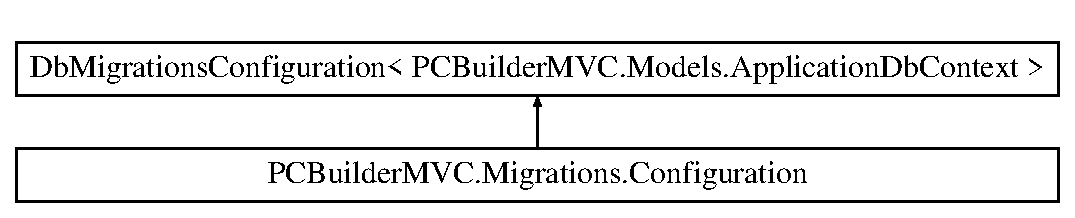
\includegraphics[height=2.000000cm]{class_p_c_builder_m_v_c_1_1_migrations_1_1_configuration}
\end{center}
\end{figure}
\subsection*{Protected Member Functions}
\begin{DoxyCompactItemize}
\item 
override void {\bfseries Seed} (\hyperlink{class_p_c_builder_m_v_c_1_1_models_1_1_application_db_context}{P\+C\+Builder\+M\+V\+C.\+Models.\+Application\+Db\+Context} context)\hypertarget{class_p_c_builder_m_v_c_1_1_migrations_1_1_configuration_ad669e0355cf96be7e84635283b055309}{}\label{class_p_c_builder_m_v_c_1_1_migrations_1_1_configuration_ad669e0355cf96be7e84635283b055309}

\end{DoxyCompactItemize}


\subsection{Detailed Description}


Definition at line 8 of file Configuration.\+cs.



The documentation for this class was generated from the following file\+:\begin{DoxyCompactItemize}
\item 
C\+:/\+Users/nh228u08/\+Desktop/\+Final\+Project/\+Final\+Project/\+P\+C\+Builder/\+P\+C\+Builder\+M\+V\+C/\+Migrations/Configuration.\+cs\end{DoxyCompactItemize}

\hypertarget{class_business_objects_1_1_c_p_u}{}\section{Business\+Objects.\+C\+PU Class Reference}
\label{class_business_objects_1_1_c_p_u}\index{Business\+Objects.\+C\+PU@{Business\+Objects.\+C\+PU}}


\hyperlink{class_business_objects_1_1_c_p_u}{C\+PU} object to hold necessary data on the \hyperlink{class_business_objects_1_1_c_p_u}{C\+PU}.  


\subsection*{Public Member Functions}
\begin{DoxyCompactItemize}
\item 
\hyperlink{class_business_objects_1_1_c_p_u_add17fa319f02b438c60fddf8e0d6a787}{C\+PU} ()
\begin{DoxyCompactList}\small\item\em Initializes a new instance of the \hyperlink{class_business_objects_1_1_c_p_u}{C\+PU} class. \end{DoxyCompactList}\item 
\hyperlink{class_business_objects_1_1_c_p_u_a13061cd0fcc98d43aa1d2c2cc63a836f}{C\+PU} (int cpu\+Id, string brand, string model, int cores, bool hyper\+Threaded, double clock\+Speed, bool unlocked, string socket, string product\+Line\+Name, int benchmark\+Score, string best\+Use, int power\+Requirement, decimal price)
\begin{DoxyCompactList}\small\item\em Initializes a new instance of the \hyperlink{class_business_objects_1_1_c_p_u}{C\+PU} class. \end{DoxyCompactList}\end{DoxyCompactItemize}
\subsection*{Properties}
\begin{DoxyCompactItemize}
\item 
int {\bfseries Cpu\+Id}\hspace{0.3cm}{\ttfamily  \mbox{[}get, set\mbox{]}}\hypertarget{class_business_objects_1_1_c_p_u_a70a9588363dcc4cb7f13d17f5027a151}{}\label{class_business_objects_1_1_c_p_u_a70a9588363dcc4cb7f13d17f5027a151}

\item 
string {\bfseries Brand}\hspace{0.3cm}{\ttfamily  \mbox{[}get, set\mbox{]}}\hypertarget{class_business_objects_1_1_c_p_u_a3bd156aa06e6fabfc82b4c0ac700f669}{}\label{class_business_objects_1_1_c_p_u_a3bd156aa06e6fabfc82b4c0ac700f669}

\item 
string {\bfseries Model}\hspace{0.3cm}{\ttfamily  \mbox{[}get, set\mbox{]}}\hypertarget{class_business_objects_1_1_c_p_u_adf6f65c8a4722dd2b6bc9c834a0efc83}{}\label{class_business_objects_1_1_c_p_u_adf6f65c8a4722dd2b6bc9c834a0efc83}

\item 
int {\bfseries Cores}\hspace{0.3cm}{\ttfamily  \mbox{[}get, set\mbox{]}}\hypertarget{class_business_objects_1_1_c_p_u_a6b71708968098064617860d9c37caaf3}{}\label{class_business_objects_1_1_c_p_u_a6b71708968098064617860d9c37caaf3}

\item 
bool {\bfseries Hyper\+Threaded}\hspace{0.3cm}{\ttfamily  \mbox{[}get, set\mbox{]}}\hypertarget{class_business_objects_1_1_c_p_u_af77e1c12c179b8411f5516eb62173df8}{}\label{class_business_objects_1_1_c_p_u_af77e1c12c179b8411f5516eb62173df8}

\item 
double {\bfseries Clock\+Speed}\hspace{0.3cm}{\ttfamily  \mbox{[}get, set\mbox{]}}\hypertarget{class_business_objects_1_1_c_p_u_a0c502313085374d20bce7c97b2635616}{}\label{class_business_objects_1_1_c_p_u_a0c502313085374d20bce7c97b2635616}

\item 
bool {\bfseries Unlocked}\hspace{0.3cm}{\ttfamily  \mbox{[}get, set\mbox{]}}\hypertarget{class_business_objects_1_1_c_p_u_a57c5e303abfa3d05ea6e54732184f355}{}\label{class_business_objects_1_1_c_p_u_a57c5e303abfa3d05ea6e54732184f355}

\item 
string {\bfseries Socket}\hspace{0.3cm}{\ttfamily  \mbox{[}get, set\mbox{]}}\hypertarget{class_business_objects_1_1_c_p_u_a183b5db42a6e13f85502bc1c1b5eb400}{}\label{class_business_objects_1_1_c_p_u_a183b5db42a6e13f85502bc1c1b5eb400}

\item 
string {\bfseries Product\+Line\+Name}\hspace{0.3cm}{\ttfamily  \mbox{[}get, set\mbox{]}}\hypertarget{class_business_objects_1_1_c_p_u_a662d917f4e92682ed35625440e339ae9}{}\label{class_business_objects_1_1_c_p_u_a662d917f4e92682ed35625440e339ae9}

\item 
int {\bfseries Benchmark\+Score}\hspace{0.3cm}{\ttfamily  \mbox{[}get, set\mbox{]}}\hypertarget{class_business_objects_1_1_c_p_u_a6e97a16652352aee41163bb01b3bf205}{}\label{class_business_objects_1_1_c_p_u_a6e97a16652352aee41163bb01b3bf205}

\item 
string {\bfseries Best\+Use}\hspace{0.3cm}{\ttfamily  \mbox{[}get, set\mbox{]}}\hypertarget{class_business_objects_1_1_c_p_u_a17391b50d5f3e059feccfa16d8535388}{}\label{class_business_objects_1_1_c_p_u_a17391b50d5f3e059feccfa16d8535388}

\item 
int {\bfseries Power\+Requirement}\hspace{0.3cm}{\ttfamily  \mbox{[}get, set\mbox{]}}\hypertarget{class_business_objects_1_1_c_p_u_acca2b421cc92cd56df0545c193f6724c}{}\label{class_business_objects_1_1_c_p_u_acca2b421cc92cd56df0545c193f6724c}

\item 
decimal {\bfseries Price}\hspace{0.3cm}{\ttfamily  \mbox{[}get, set\mbox{]}}\hypertarget{class_business_objects_1_1_c_p_u_ac7f66e5df1a12f80d76f06fd969dc35e}{}\label{class_business_objects_1_1_c_p_u_ac7f66e5df1a12f80d76f06fd969dc35e}

\end{DoxyCompactItemize}


\subsection{Detailed Description}
\hyperlink{class_business_objects_1_1_c_p_u}{C\+PU} object to hold necessary data on the \hyperlink{class_business_objects_1_1_c_p_u}{C\+PU}. 



Definition at line 17 of file C\+P\+U.\+cs.



\subsection{Constructor \& Destructor Documentation}
\index{Business\+Objects\+::\+C\+PU@{Business\+Objects\+::\+C\+PU}!C\+PU@{C\+PU}}
\index{C\+PU@{C\+PU}!Business\+Objects\+::\+C\+PU@{Business\+Objects\+::\+C\+PU}}
\subsubsection[{\texorpdfstring{C\+P\+U()}{CPU()}}]{\setlength{\rightskip}{0pt plus 5cm}Business\+Objects.\+C\+P\+U.\+C\+PU (
\begin{DoxyParamCaption}
{}
\end{DoxyParamCaption}
)}\hypertarget{class_business_objects_1_1_c_p_u_add17fa319f02b438c60fddf8e0d6a787}{}\label{class_business_objects_1_1_c_p_u_add17fa319f02b438c60fddf8e0d6a787}


Initializes a new instance of the \hyperlink{class_business_objects_1_1_c_p_u}{C\+PU} class. 



Definition at line 36 of file C\+P\+U.\+cs.

\index{Business\+Objects\+::\+C\+PU@{Business\+Objects\+::\+C\+PU}!C\+PU@{C\+PU}}
\index{C\+PU@{C\+PU}!Business\+Objects\+::\+C\+PU@{Business\+Objects\+::\+C\+PU}}
\subsubsection[{\texorpdfstring{C\+P\+U(int cpu\+Id, string brand, string model, int cores, bool hyper\+Threaded, double clock\+Speed, bool unlocked, string socket, string product\+Line\+Name, int benchmark\+Score, string best\+Use, int power\+Requirement, decimal price)}{CPU(int cpuId, string brand, string model, int cores, bool hyperThreaded, double clockSpeed, bool unlocked, string socket, string productLineName, int benchmarkScore, string bestUse, int powerRequirement, decimal price)}}]{\setlength{\rightskip}{0pt plus 5cm}Business\+Objects.\+C\+P\+U.\+C\+PU (
\begin{DoxyParamCaption}
\item[{int}]{cpu\+Id, }
\item[{string}]{brand, }
\item[{string}]{model, }
\item[{int}]{cores, }
\item[{bool}]{hyper\+Threaded, }
\item[{double}]{clock\+Speed, }
\item[{bool}]{unlocked, }
\item[{string}]{socket, }
\item[{string}]{product\+Line\+Name, }
\item[{int}]{benchmark\+Score, }
\item[{string}]{best\+Use, }
\item[{int}]{power\+Requirement, }
\item[{decimal}]{price}
\end{DoxyParamCaption}
)}\hypertarget{class_business_objects_1_1_c_p_u_a13061cd0fcc98d43aa1d2c2cc63a836f}{}\label{class_business_objects_1_1_c_p_u_a13061cd0fcc98d43aa1d2c2cc63a836f}


Initializes a new instance of the \hyperlink{class_business_objects_1_1_c_p_u}{C\+PU} class. 


\begin{DoxyParams}{Parameters}
{\em cpu\+Id} & The cpu identifier.\\
\hline
{\em brand} & The brand.\\
\hline
{\em model} & The model.\\
\hline
{\em cores} & The core count.\\
\hline
{\em hyper\+Threaded} & if set to {\ttfamily true}, \mbox{[}hyper threaded\mbox{]}.\\
\hline
{\em clock\+Speed} & The clock speed.\\
\hline
{\em unlocked} & if set to {\ttfamily true}, \mbox{[}unlocked\mbox{]}.\\
\hline
{\em socket} & The socket.\\
\hline
{\em product\+Line\+Name} & Name of the product line.\\
\hline
{\em benchmark\+Score} & The benchmark score.\\
\hline
{\em best\+Use} & The best use case.\\
\hline
{\em power\+Requirement} & The power requirement.\\
\hline
{\em price} & The price.\\
\hline
\end{DoxyParams}


Definition at line 54 of file C\+P\+U.\+cs.



The documentation for this class was generated from the following file\+:\begin{DoxyCompactItemize}
\item 
C\+:/\+Users/nh228u08/\+Desktop/\+Final\+Project/\+Final\+Project/\+P\+C\+Builder/\+Business\+Objects/C\+P\+U.\+cs\end{DoxyCompactItemize}

\hypertarget{class_p_c_builder_m_v_c_1_1_models_1_1_c_p_u}{}\section{P\+C\+Builder\+M\+V\+C.\+Models.\+C\+PU Class Reference}
\label{class_p_c_builder_m_v_c_1_1_models_1_1_c_p_u}\index{P\+C\+Builder\+M\+V\+C.\+Models.\+C\+PU@{P\+C\+Builder\+M\+V\+C.\+Models.\+C\+PU}}


\hyperlink{class_p_c_builder_m_v_c_1_1_models_1_1_c_p_u}{C\+PU} view model class.  


\subsection*{Properties}
\begin{DoxyCompactItemize}
\item 
int {\bfseries Cpu\+Id}\hspace{0.3cm}{\ttfamily  \mbox{[}get, set\mbox{]}}\hypertarget{class_p_c_builder_m_v_c_1_1_models_1_1_c_p_u_a990a746196bffb0de705df0e5d05a5f3}{}\label{class_p_c_builder_m_v_c_1_1_models_1_1_c_p_u_a990a746196bffb0de705df0e5d05a5f3}

\item 
string {\bfseries Brand}\hspace{0.3cm}{\ttfamily  \mbox{[}get, set\mbox{]}}\hypertarget{class_p_c_builder_m_v_c_1_1_models_1_1_c_p_u_a46f0933a115043582379ed8845692090}{}\label{class_p_c_builder_m_v_c_1_1_models_1_1_c_p_u_a46f0933a115043582379ed8845692090}

\item 
string {\bfseries Model}\hspace{0.3cm}{\ttfamily  \mbox{[}get, set\mbox{]}}\hypertarget{class_p_c_builder_m_v_c_1_1_models_1_1_c_p_u_a64cd925d1ab719b2c4519d314c11ae7a}{}\label{class_p_c_builder_m_v_c_1_1_models_1_1_c_p_u_a64cd925d1ab719b2c4519d314c11ae7a}

\item 
int {\bfseries Cores}\hspace{0.3cm}{\ttfamily  \mbox{[}get, set\mbox{]}}\hypertarget{class_p_c_builder_m_v_c_1_1_models_1_1_c_p_u_a3b51ddcaba446375f2880e448d22d66f}{}\label{class_p_c_builder_m_v_c_1_1_models_1_1_c_p_u_a3b51ddcaba446375f2880e448d22d66f}

\item 
bool {\bfseries Hyper\+Threaded}\hspace{0.3cm}{\ttfamily  \mbox{[}get, set\mbox{]}}\hypertarget{class_p_c_builder_m_v_c_1_1_models_1_1_c_p_u_a4e09d178413e4af0f20b39f275f06591}{}\label{class_p_c_builder_m_v_c_1_1_models_1_1_c_p_u_a4e09d178413e4af0f20b39f275f06591}

\item 
double {\bfseries Clock\+Speed}\hspace{0.3cm}{\ttfamily  \mbox{[}get, set\mbox{]}}\hypertarget{class_p_c_builder_m_v_c_1_1_models_1_1_c_p_u_a3b88315bd4c8d296807d3f38f6f705f8}{}\label{class_p_c_builder_m_v_c_1_1_models_1_1_c_p_u_a3b88315bd4c8d296807d3f38f6f705f8}

\item 
bool {\bfseries Unlocked}\hspace{0.3cm}{\ttfamily  \mbox{[}get, set\mbox{]}}\hypertarget{class_p_c_builder_m_v_c_1_1_models_1_1_c_p_u_ad2e6b5def809796f3a7865ea0be5f22b}{}\label{class_p_c_builder_m_v_c_1_1_models_1_1_c_p_u_ad2e6b5def809796f3a7865ea0be5f22b}

\item 
string {\bfseries Socket}\hspace{0.3cm}{\ttfamily  \mbox{[}get, set\mbox{]}}\hypertarget{class_p_c_builder_m_v_c_1_1_models_1_1_c_p_u_a12d3226172e4f56916215600f3e396e5}{}\label{class_p_c_builder_m_v_c_1_1_models_1_1_c_p_u_a12d3226172e4f56916215600f3e396e5}

\item 
string {\bfseries Product\+Line\+Name}\hspace{0.3cm}{\ttfamily  \mbox{[}get, set\mbox{]}}\hypertarget{class_p_c_builder_m_v_c_1_1_models_1_1_c_p_u_adf3f7a5d8ab10033237a18ae9b68437c}{}\label{class_p_c_builder_m_v_c_1_1_models_1_1_c_p_u_adf3f7a5d8ab10033237a18ae9b68437c}

\item 
int {\bfseries Benchmark\+Score}\hspace{0.3cm}{\ttfamily  \mbox{[}get, set\mbox{]}}\hypertarget{class_p_c_builder_m_v_c_1_1_models_1_1_c_p_u_a4061ea1754a5439a260d290f642d1eaf}{}\label{class_p_c_builder_m_v_c_1_1_models_1_1_c_p_u_a4061ea1754a5439a260d290f642d1eaf}

\item 
string {\bfseries Best\+Use}\hspace{0.3cm}{\ttfamily  \mbox{[}get, set\mbox{]}}\hypertarget{class_p_c_builder_m_v_c_1_1_models_1_1_c_p_u_ad2680d0499c84545de6787a7a185c7d8}{}\label{class_p_c_builder_m_v_c_1_1_models_1_1_c_p_u_ad2680d0499c84545de6787a7a185c7d8}

\item 
int {\bfseries Power\+Requirement}\hspace{0.3cm}{\ttfamily  \mbox{[}get, set\mbox{]}}\hypertarget{class_p_c_builder_m_v_c_1_1_models_1_1_c_p_u_a8c71bc85082460aa45e7bc30bf90c477}{}\label{class_p_c_builder_m_v_c_1_1_models_1_1_c_p_u_a8c71bc85082460aa45e7bc30bf90c477}

\item 
decimal {\bfseries Price}\hspace{0.3cm}{\ttfamily  \mbox{[}get, set\mbox{]}}\hypertarget{class_p_c_builder_m_v_c_1_1_models_1_1_c_p_u_a456c4cc415062456a8b8b3b1fc61b077}{}\label{class_p_c_builder_m_v_c_1_1_models_1_1_c_p_u_a456c4cc415062456a8b8b3b1fc61b077}

\end{DoxyCompactItemize}


\subsection{Detailed Description}
\hyperlink{class_p_c_builder_m_v_c_1_1_models_1_1_c_p_u}{C\+PU} view model class. 



Definition at line 13 of file C\+P\+U.\+cs.



The documentation for this class was generated from the following file\+:\begin{DoxyCompactItemize}
\item 
C\+:/\+Users/nh228u08/\+Desktop/\+Final\+Project/\+Final\+Project/\+P\+C\+Builder/\+P\+C\+Builder\+M\+V\+C/\+Models/C\+P\+U.\+cs\end{DoxyCompactItemize}

\hypertarget{class_data_access_1_1_c_p_u_accessor}{}\section{Data\+Access.\+C\+P\+U\+Accessor Class Reference}
\label{class_data_access_1_1_c_p_u_accessor}\index{Data\+Access.\+C\+P\+U\+Accessor@{Data\+Access.\+C\+P\+U\+Accessor}}


C\+PU accessor to communicate with database on C\+PU objects.  


\subsection*{Static Public Member Functions}
\begin{DoxyCompactItemize}
\item 
static \hyperlink{class_business_objects_1_1_c_p_u}{C\+PU} \hyperlink{class_data_access_1_1_c_p_u_accessor_a92d43c1a282b8bbaf39e48514f9a54e7}{Retrieve\+C\+P\+U\+By\+Name} (string name)
\begin{DoxyCompactList}\small\item\em Retrieves a C\+PU by name. \end{DoxyCompactList}\item 
static List$<$ \hyperlink{class_business_objects_1_1_c_p_u}{C\+PU} $>$ \hyperlink{class_data_access_1_1_c_p_u_accessor_a07c977d60ddb3c98a6de06c2b74f3129}{Retrieve\+C\+P\+Us\+By\+Core\+Count} (int cores)
\begin{DoxyCompactList}\small\item\em Retrieves C\+P\+Us by core count. \end{DoxyCompactList}\item 
static int \hyperlink{class_data_access_1_1_c_p_u_accessor_a3bdc9307783a16d68413e856e2be24ee}{Insert\+Cpu} (\hyperlink{class_business_objects_1_1_c_p_u}{C\+PU} cpu)
\begin{DoxyCompactList}\small\item\em Inserts a new C\+PU. \end{DoxyCompactList}\item 
static List$<$ \hyperlink{class_business_objects_1_1_c_p_u}{C\+PU} $>$ \hyperlink{class_data_access_1_1_c_p_u_accessor_af33b1affd73312b1cad5637dd2f66aec}{Retrieve\+All\+C\+PU} ()
\begin{DoxyCompactList}\small\item\em Retrieves all C\+P\+Us. \end{DoxyCompactList}\end{DoxyCompactItemize}


\subsection{Detailed Description}
C\+PU accessor to communicate with database on C\+PU objects. 



Definition at line 15 of file C\+P\+U\+Accessor.\+cs.



\subsection{Member Function Documentation}
\index{Data\+Access\+::\+C\+P\+U\+Accessor@{Data\+Access\+::\+C\+P\+U\+Accessor}!Insert\+Cpu@{Insert\+Cpu}}
\index{Insert\+Cpu@{Insert\+Cpu}!Data\+Access\+::\+C\+P\+U\+Accessor@{Data\+Access\+::\+C\+P\+U\+Accessor}}
\subsubsection[{\texorpdfstring{Insert\+Cpu(\+C\+P\+U cpu)}{InsertCpu(CPU cpu)}}]{\setlength{\rightskip}{0pt plus 5cm}static int Data\+Access.\+C\+P\+U\+Accessor.\+Insert\+Cpu (
\begin{DoxyParamCaption}
\item[{{\bf C\+PU}}]{cpu}
\end{DoxyParamCaption}
)\hspace{0.3cm}{\ttfamily [static]}}\hypertarget{class_data_access_1_1_c_p_u_accessor_a3bdc9307783a16d68413e856e2be24ee}{}\label{class_data_access_1_1_c_p_u_accessor_a3bdc9307783a16d68413e856e2be24ee}


Inserts a new C\+PU. 


\begin{DoxyParams}{Parameters}
{\em cpu} & The cpu.\\
\hline
\end{DoxyParams}
\begin{DoxyReturn}{Returns}
Count of rows affected.
\end{DoxyReturn}


Definition at line 137 of file C\+P\+U\+Accessor.\+cs.

\index{Data\+Access\+::\+C\+P\+U\+Accessor@{Data\+Access\+::\+C\+P\+U\+Accessor}!Retrieve\+All\+C\+PU@{Retrieve\+All\+C\+PU}}
\index{Retrieve\+All\+C\+PU@{Retrieve\+All\+C\+PU}!Data\+Access\+::\+C\+P\+U\+Accessor@{Data\+Access\+::\+C\+P\+U\+Accessor}}
\subsubsection[{\texorpdfstring{Retrieve\+All\+C\+P\+U()}{RetrieveAllCPU()}}]{\setlength{\rightskip}{0pt plus 5cm}static List$<${\bf C\+PU}$>$ Data\+Access.\+C\+P\+U\+Accessor.\+Retrieve\+All\+C\+PU (
\begin{DoxyParamCaption}
{}
\end{DoxyParamCaption}
)\hspace{0.3cm}{\ttfamily [static]}}\hypertarget{class_data_access_1_1_c_p_u_accessor_af33b1affd73312b1cad5637dd2f66aec}{}\label{class_data_access_1_1_c_p_u_accessor_af33b1affd73312b1cad5637dd2f66aec}


Retrieves all C\+P\+Us. 

\begin{DoxyReturn}{Returns}
Lsit of C\+PU objects.
\end{DoxyReturn}

\begin{DoxyExceptions}{Exceptions}
{\em System.\+Application\+Exception} & Data not found.\\
\hline
\end{DoxyExceptions}


Definition at line 182 of file C\+P\+U\+Accessor.\+cs.

\index{Data\+Access\+::\+C\+P\+U\+Accessor@{Data\+Access\+::\+C\+P\+U\+Accessor}!Retrieve\+C\+P\+U\+By\+Name@{Retrieve\+C\+P\+U\+By\+Name}}
\index{Retrieve\+C\+P\+U\+By\+Name@{Retrieve\+C\+P\+U\+By\+Name}!Data\+Access\+::\+C\+P\+U\+Accessor@{Data\+Access\+::\+C\+P\+U\+Accessor}}
\subsubsection[{\texorpdfstring{Retrieve\+C\+P\+U\+By\+Name(string name)}{RetrieveCPUByName(string name)}}]{\setlength{\rightskip}{0pt plus 5cm}static {\bf C\+PU} Data\+Access.\+C\+P\+U\+Accessor.\+Retrieve\+C\+P\+U\+By\+Name (
\begin{DoxyParamCaption}
\item[{string}]{name}
\end{DoxyParamCaption}
)\hspace{0.3cm}{\ttfamily [static]}}\hypertarget{class_data_access_1_1_c_p_u_accessor_a92d43c1a282b8bbaf39e48514f9a54e7}{}\label{class_data_access_1_1_c_p_u_accessor_a92d43c1a282b8bbaf39e48514f9a54e7}


Retrieves a C\+PU by name. 


\begin{DoxyParams}{Parameters}
{\em name} & The name.\\
\hline
\end{DoxyParams}
\begin{DoxyReturn}{Returns}
C\+PU object.
\end{DoxyReturn}

\begin{DoxyExceptions}{Exceptions}
{\em System.\+Application\+Exception} & Data not found\\
\hline
\end{DoxyExceptions}


Definition at line 23 of file C\+P\+U\+Accessor.\+cs.

\index{Data\+Access\+::\+C\+P\+U\+Accessor@{Data\+Access\+::\+C\+P\+U\+Accessor}!Retrieve\+C\+P\+Us\+By\+Core\+Count@{Retrieve\+C\+P\+Us\+By\+Core\+Count}}
\index{Retrieve\+C\+P\+Us\+By\+Core\+Count@{Retrieve\+C\+P\+Us\+By\+Core\+Count}!Data\+Access\+::\+C\+P\+U\+Accessor@{Data\+Access\+::\+C\+P\+U\+Accessor}}
\subsubsection[{\texorpdfstring{Retrieve\+C\+P\+Us\+By\+Core\+Count(int cores)}{RetrieveCPUsByCoreCount(int cores)}}]{\setlength{\rightskip}{0pt plus 5cm}static List$<${\bf C\+PU}$>$ Data\+Access.\+C\+P\+U\+Accessor.\+Retrieve\+C\+P\+Us\+By\+Core\+Count (
\begin{DoxyParamCaption}
\item[{int}]{cores}
\end{DoxyParamCaption}
)\hspace{0.3cm}{\ttfamily [static]}}\hypertarget{class_data_access_1_1_c_p_u_accessor_a07c977d60ddb3c98a6de06c2b74f3129}{}\label{class_data_access_1_1_c_p_u_accessor_a07c977d60ddb3c98a6de06c2b74f3129}


Retrieves C\+P\+Us by core count. 


\begin{DoxyParams}{Parameters}
{\em cores} & The cores.\\
\hline
\end{DoxyParams}
\begin{DoxyReturn}{Returns}
List of C\+PU objects.
\end{DoxyReturn}

\begin{DoxyExceptions}{Exceptions}
{\em System.\+Application\+Exception} & Data not found\\
\hline
\end{DoxyExceptions}


Definition at line 80 of file C\+P\+U\+Accessor.\+cs.



The documentation for this class was generated from the following file\+:\begin{DoxyCompactItemize}
\item 
C\+:/\+Users/nh228u08/\+Desktop/\+Final\+Project/\+Final\+Project/\+P\+C\+Builder/\+Data\+Access/C\+P\+U\+Accessor.\+cs\end{DoxyCompactItemize}

\hypertarget{class_p_c_builder_m_v_c_1_1_controllers_1_1_c_p_u_controller}{}\section{P\+C\+Builder\+M\+V\+C.\+Controllers.\+C\+P\+U\+Controller Class Reference}
\label{class_p_c_builder_m_v_c_1_1_controllers_1_1_c_p_u_controller}\index{P\+C\+Builder\+M\+V\+C.\+Controllers.\+C\+P\+U\+Controller@{P\+C\+Builder\+M\+V\+C.\+Controllers.\+C\+P\+U\+Controller}}


C\+PU controller class to handle C\+PU views interaction.  


Inheritance diagram for P\+C\+Builder\+M\+V\+C.\+Controllers.\+C\+P\+U\+Controller\+:\begin{figure}[H]
\begin{center}
\leavevmode
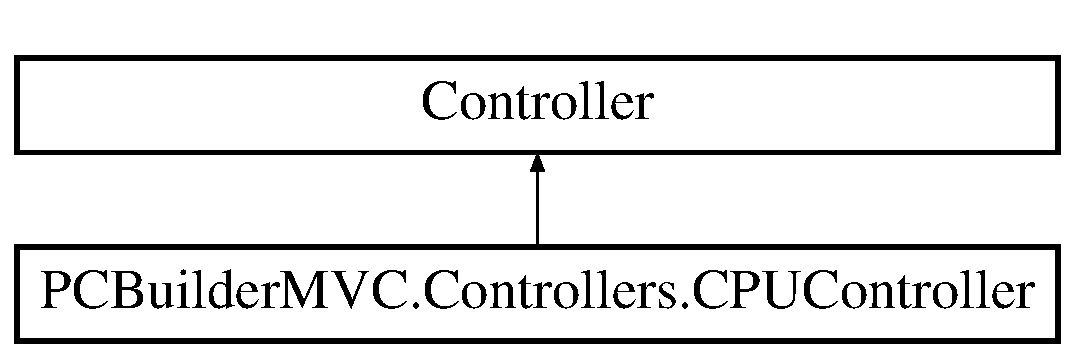
\includegraphics[height=2.000000cm]{class_p_c_builder_m_v_c_1_1_controllers_1_1_c_p_u_controller}
\end{center}
\end{figure}
\subsection*{Public Member Functions}
\begin{DoxyCompactItemize}
\item 
Action\+Result {\bfseries Index} ()\hypertarget{class_p_c_builder_m_v_c_1_1_controllers_1_1_c_p_u_controller_aa640d493ea48a0ed025e6c2c98d083f0}{}\label{class_p_c_builder_m_v_c_1_1_controllers_1_1_c_p_u_controller_aa640d493ea48a0ed025e6c2c98d083f0}

\item 
Action\+Result {\bfseries Details} (int?id)\hypertarget{class_p_c_builder_m_v_c_1_1_controllers_1_1_c_p_u_controller_a4d6de4531fcd3eaad2980fe9741743c0}{}\label{class_p_c_builder_m_v_c_1_1_controllers_1_1_c_p_u_controller_a4d6de4531fcd3eaad2980fe9741743c0}

\item 
Action\+Result {\bfseries Create} ()\hypertarget{class_p_c_builder_m_v_c_1_1_controllers_1_1_c_p_u_controller_acd679be1eb43977d5f4b3929083cbc55}{}\label{class_p_c_builder_m_v_c_1_1_controllers_1_1_c_p_u_controller_acd679be1eb43977d5f4b3929083cbc55}

\item 
Action\+Result {\bfseries Create} (\mbox{[}Bind(Include=\char`\"{}Cpu\+Id,Brand,Model,Cores,Hyper\+Threaded,Clock\+Speed,Unlocked,Socket,Product\+Line\+Name,Benchmark\+Score,Best\+Use,Power\+Requirement,Price\char`\"{})\mbox{]} C\+PU c\+PU)\hypertarget{class_p_c_builder_m_v_c_1_1_controllers_1_1_c_p_u_controller_ac04207e76257b362078c5f18a11a7d11}{}\label{class_p_c_builder_m_v_c_1_1_controllers_1_1_c_p_u_controller_ac04207e76257b362078c5f18a11a7d11}

\item 
Action\+Result {\bfseries Edit} (int?id)\hypertarget{class_p_c_builder_m_v_c_1_1_controllers_1_1_c_p_u_controller_a3c8e98d63f6196a2e8f4e254dba66ce5}{}\label{class_p_c_builder_m_v_c_1_1_controllers_1_1_c_p_u_controller_a3c8e98d63f6196a2e8f4e254dba66ce5}

\item 
Action\+Result {\bfseries Edit} (\mbox{[}Bind(Include=\char`\"{}Cpu\+Id,Brand,Model,Cores,Hyper\+Threaded,Clock\+Speed,Unlocked,Socket,Product\+Line\+Name,Benchmark\+Score,Best\+Use,Power\+Requirement,Price\char`\"{})\mbox{]} C\+PU c\+PU)\hypertarget{class_p_c_builder_m_v_c_1_1_controllers_1_1_c_p_u_controller_a1bf99839d52ca6ad02e971feb0f0ad4b}{}\label{class_p_c_builder_m_v_c_1_1_controllers_1_1_c_p_u_controller_a1bf99839d52ca6ad02e971feb0f0ad4b}

\item 
Action\+Result {\bfseries Delete} (int?id)\hypertarget{class_p_c_builder_m_v_c_1_1_controllers_1_1_c_p_u_controller_aecf48e4974303f62bfc5df8ffee64c7b}{}\label{class_p_c_builder_m_v_c_1_1_controllers_1_1_c_p_u_controller_aecf48e4974303f62bfc5df8ffee64c7b}

\item 
Action\+Result {\bfseries Delete\+Confirmed} (int id)\hypertarget{class_p_c_builder_m_v_c_1_1_controllers_1_1_c_p_u_controller_aae1ff81c3b6e4e5ba3b1ac03106a7ed2}{}\label{class_p_c_builder_m_v_c_1_1_controllers_1_1_c_p_u_controller_aae1ff81c3b6e4e5ba3b1ac03106a7ed2}

\end{DoxyCompactItemize}
\subsection*{Protected Member Functions}
\begin{DoxyCompactItemize}
\item 
override void {\bfseries Dispose} (bool disposing)\hypertarget{class_p_c_builder_m_v_c_1_1_controllers_1_1_c_p_u_controller_a3b3148ca684258dc2d3a75ef1abc005e}{}\label{class_p_c_builder_m_v_c_1_1_controllers_1_1_c_p_u_controller_a3b3148ca684258dc2d3a75ef1abc005e}

\end{DoxyCompactItemize}
\subsection*{Private Attributes}
\begin{DoxyCompactItemize}
\item 
\hyperlink{class_p_c_builder_m_v_c_1_1_models_1_1_p_c_builder_entity_models}{P\+C\+Builder\+Entity\+Models} {\bfseries db} = new \hyperlink{class_p_c_builder_m_v_c_1_1_models_1_1_p_c_builder_entity_models}{P\+C\+Builder\+Entity\+Models}()\hypertarget{class_p_c_builder_m_v_c_1_1_controllers_1_1_c_p_u_controller_a77284533fab5d9ff56207220384cadf7}{}\label{class_p_c_builder_m_v_c_1_1_controllers_1_1_c_p_u_controller_a77284533fab5d9ff56207220384cadf7}

\end{DoxyCompactItemize}


\subsection{Detailed Description}
C\+PU controller class to handle C\+PU views interaction. 

\begin{DoxySeeAlso}{See also}
System.\+Web.\+Mvc.\+Controller


\end{DoxySeeAlso}


Definition at line 17 of file C\+P\+U\+Controller.\+cs.



The documentation for this class was generated from the following file\+:\begin{DoxyCompactItemize}
\item 
C\+:/\+Users/nh228u08/\+Desktop/\+Final\+Project/\+Final\+Project/\+P\+C\+Builder/\+P\+C\+Builder\+M\+V\+C/\+Controllers/C\+P\+U\+Controller.\+cs\end{DoxyCompactItemize}

\hypertarget{class_data_access_1_1_d_b_connection}{}\section{Data\+Access.\+D\+B\+Connection Class Reference}
\label{class_data_access_1_1_d_b_connection}\index{Data\+Access.\+D\+B\+Connection@{Data\+Access.\+D\+B\+Connection}}


Database connector string class.  


\subsection*{Static Public Member Functions}
\begin{DoxyCompactItemize}
\item 
static Sql\+Connection \hyperlink{class_data_access_1_1_d_b_connection_acb22adf9b3f24c80a2b81ec2d1919718}{Get\+D\+B\+Connection} ()
\begin{DoxyCompactList}\small\item\em Gets the database connection. \end{DoxyCompactList}\end{DoxyCompactItemize}
\subsection*{Private Attributes}
\begin{DoxyCompactItemize}
\item 
const string \hyperlink{class_data_access_1_1_d_b_connection_ada2203b451d5a83a7e566970443846ea}{Connection\+String} = @\char`\"{}Data Source=localhost;Initial Catalog=P\+C\+Builder;Integrated Security=True\char`\"{}
\begin{DoxyCompactList}\small\item\em The connection string \end{DoxyCompactList}\end{DoxyCompactItemize}


\subsection{Detailed Description}
Database connector string class. 



Definition at line 13 of file D\+B\+Connection.\+cs.



\subsection{Member Function Documentation}
\index{Data\+Access\+::\+D\+B\+Connection@{Data\+Access\+::\+D\+B\+Connection}!Get\+D\+B\+Connection@{Get\+D\+B\+Connection}}
\index{Get\+D\+B\+Connection@{Get\+D\+B\+Connection}!Data\+Access\+::\+D\+B\+Connection@{Data\+Access\+::\+D\+B\+Connection}}
\subsubsection[{\texorpdfstring{Get\+D\+B\+Connection()}{GetDBConnection()}}]{\setlength{\rightskip}{0pt plus 5cm}static Sql\+Connection Data\+Access.\+D\+B\+Connection.\+Get\+D\+B\+Connection (
\begin{DoxyParamCaption}
{}
\end{DoxyParamCaption}
)\hspace{0.3cm}{\ttfamily [static]}}\hypertarget{class_data_access_1_1_d_b_connection_acb22adf9b3f24c80a2b81ec2d1919718}{}\label{class_data_access_1_1_d_b_connection_acb22adf9b3f24c80a2b81ec2d1919718}


Gets the database connection. 

\begin{DoxyReturn}{Returns}
Sql\+Connection object.
\end{DoxyReturn}


Definition at line 24 of file D\+B\+Connection.\+cs.



\subsection{Member Data Documentation}
\index{Data\+Access\+::\+D\+B\+Connection@{Data\+Access\+::\+D\+B\+Connection}!Connection\+String@{Connection\+String}}
\index{Connection\+String@{Connection\+String}!Data\+Access\+::\+D\+B\+Connection@{Data\+Access\+::\+D\+B\+Connection}}
\subsubsection[{\texorpdfstring{Connection\+String}{ConnectionString}}]{\setlength{\rightskip}{0pt plus 5cm}const string Data\+Access.\+D\+B\+Connection.\+Connection\+String = @\char`\"{}Data Source=localhost;Initial Catalog=P\+C\+Builder;Integrated Security=True\char`\"{}\hspace{0.3cm}{\ttfamily [private]}}\hypertarget{class_data_access_1_1_d_b_connection_ada2203b451d5a83a7e566970443846ea}{}\label{class_data_access_1_1_d_b_connection_ada2203b451d5a83a7e566970443846ea}


The connection string 



Definition at line 18 of file D\+B\+Connection.\+cs.



The documentation for this class was generated from the following file\+:\begin{DoxyCompactItemize}
\item 
C\+:/\+Users/nh228u08/\+Desktop/\+Final\+Project/\+Final\+Project/\+P\+C\+Builder/\+Data\+Access/D\+B\+Connection.\+cs\end{DoxyCompactItemize}

\hypertarget{class_p_c_builder_m_v_c_1_1_migrations_1_1dbupdate1}{}\section{P\+C\+Builder\+M\+V\+C.\+Migrations.\+dbupdate1 Class Reference}
\label{class_p_c_builder_m_v_c_1_1_migrations_1_1dbupdate1}\index{P\+C\+Builder\+M\+V\+C.\+Migrations.\+dbupdate1@{P\+C\+Builder\+M\+V\+C.\+Migrations.\+dbupdate1}}
Inheritance diagram for P\+C\+Builder\+M\+V\+C.\+Migrations.\+dbupdate1\+:\begin{figure}[H]
\begin{center}
\leavevmode
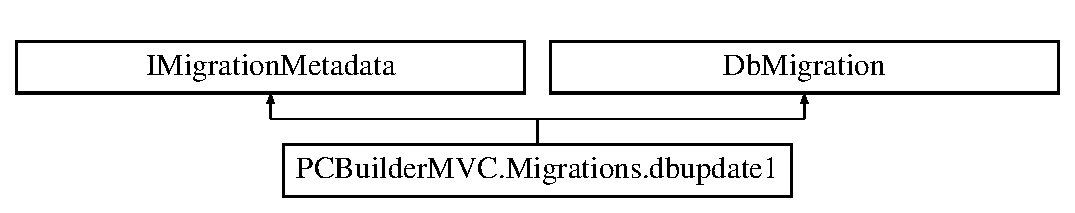
\includegraphics[height=2.000000cm]{class_p_c_builder_m_v_c_1_1_migrations_1_1dbupdate1}
\end{center}
\end{figure}
\subsection*{Public Member Functions}
\begin{DoxyCompactItemize}
\item 
override void {\bfseries Up} ()\hypertarget{class_p_c_builder_m_v_c_1_1_migrations_1_1dbupdate1_a1f02ce7d271ad7cdae7162c82dd946fb}{}\label{class_p_c_builder_m_v_c_1_1_migrations_1_1dbupdate1_a1f02ce7d271ad7cdae7162c82dd946fb}

\item 
override void {\bfseries Down} ()\hypertarget{class_p_c_builder_m_v_c_1_1_migrations_1_1dbupdate1_ac88cfe63fdfe3dc33eaabe795ac754d3}{}\label{class_p_c_builder_m_v_c_1_1_migrations_1_1dbupdate1_ac88cfe63fdfe3dc33eaabe795ac754d3}

\end{DoxyCompactItemize}
\subsection*{Properties}
\begin{DoxyCompactItemize}
\item 
string I\+Migration\+Metadata. {\bfseries Id}\hspace{0.3cm}{\ttfamily  \mbox{[}get\mbox{]}}\hypertarget{class_p_c_builder_m_v_c_1_1_migrations_1_1dbupdate1_afd8913f5a916c8efa3b3ae38c6ccc16e}{}\label{class_p_c_builder_m_v_c_1_1_migrations_1_1dbupdate1_afd8913f5a916c8efa3b3ae38c6ccc16e}

\item 
string I\+Migration\+Metadata. {\bfseries Source}\hspace{0.3cm}{\ttfamily  \mbox{[}get\mbox{]}}\hypertarget{class_p_c_builder_m_v_c_1_1_migrations_1_1dbupdate1_a1715c8c609433727839abed592e73a5e}{}\label{class_p_c_builder_m_v_c_1_1_migrations_1_1dbupdate1_a1715c8c609433727839abed592e73a5e}

\item 
string I\+Migration\+Metadata. {\bfseries Target}\hspace{0.3cm}{\ttfamily  \mbox{[}get\mbox{]}}\hypertarget{class_p_c_builder_m_v_c_1_1_migrations_1_1dbupdate1_a359a47c990e68ea3cf87e97297ca5653}{}\label{class_p_c_builder_m_v_c_1_1_migrations_1_1dbupdate1_a359a47c990e68ea3cf87e97297ca5653}

\end{DoxyCompactItemize}
\subsection*{Private Attributes}
\begin{DoxyCompactItemize}
\item 
readonly Resource\+Manager {\bfseries Resources} = new Resource\+Manager(typeof(\hyperlink{class_p_c_builder_m_v_c_1_1_migrations_1_1dbupdate1}{dbupdate1}))\hypertarget{class_p_c_builder_m_v_c_1_1_migrations_1_1dbupdate1_a52d5952868fe61cb9dfc9770284097c3}{}\label{class_p_c_builder_m_v_c_1_1_migrations_1_1dbupdate1_a52d5952868fe61cb9dfc9770284097c3}

\end{DoxyCompactItemize}


\subsection{Detailed Description}


Definition at line 6 of file 201605042345510\+\_\+dbupdate1.\+cs.



The documentation for this class was generated from the following files\+:\begin{DoxyCompactItemize}
\item 
C\+:/\+Users/nh228u08/\+Desktop/\+Final\+Project/\+Final\+Project/\+P\+C\+Builder/\+P\+C\+Builder\+M\+V\+C/\+Migrations/201605042345510\+\_\+dbupdate1.\+cs\item 
C\+:/\+Users/nh228u08/\+Desktop/\+Final\+Project/\+Final\+Project/\+P\+C\+Builder/\+P\+C\+Builder\+M\+V\+C/\+Migrations/201605042345510\+\_\+dbupdate1.\+Designer.\+cs\end{DoxyCompactItemize}

\hypertarget{class_p_c_builder_m_v_c_1_1_email_service}{}\section{P\+C\+Builder\+M\+V\+C.\+Email\+Service Class Reference}
\label{class_p_c_builder_m_v_c_1_1_email_service}\index{P\+C\+Builder\+M\+V\+C.\+Email\+Service@{P\+C\+Builder\+M\+V\+C.\+Email\+Service}}


Creates an email service.  


Inheritance diagram for P\+C\+Builder\+M\+V\+C.\+Email\+Service\+:\begin{figure}[H]
\begin{center}
\leavevmode
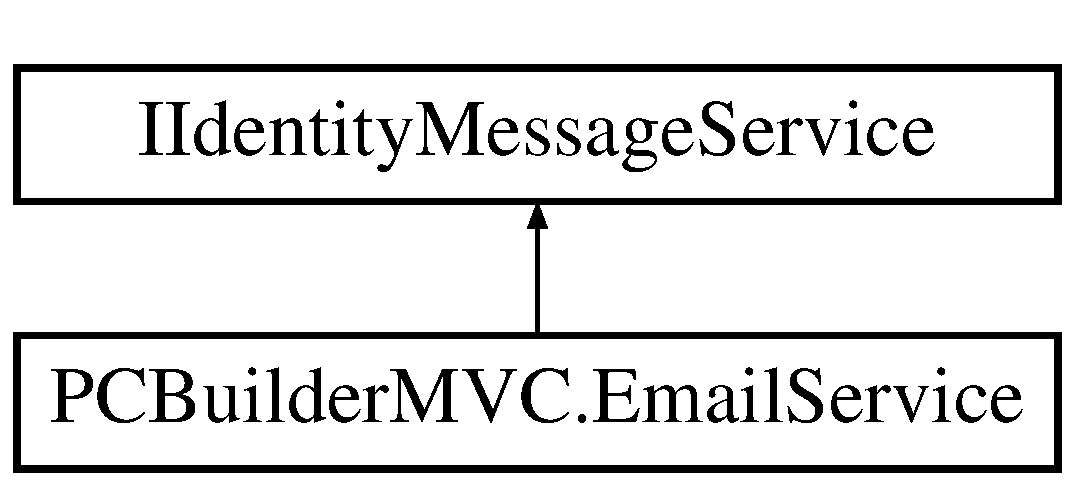
\includegraphics[height=2.000000cm]{class_p_c_builder_m_v_c_1_1_email_service}
\end{center}
\end{figure}
\subsection*{Public Member Functions}
\begin{DoxyCompactItemize}
\item 
Task {\bfseries Send\+Async} (Identity\+Message message)\hypertarget{class_p_c_builder_m_v_c_1_1_email_service_a5edc6da9b4227c6f699f71c011c86621}{}\label{class_p_c_builder_m_v_c_1_1_email_service_a5edc6da9b4227c6f699f71c011c86621}

\end{DoxyCompactItemize}


\subsection{Detailed Description}
Creates an email service. 

\begin{DoxySeeAlso}{See also}
Microsoft.\+Asp\+Net.\+Identity.\+I\+Identity\+Message\+Service


\end{DoxySeeAlso}


Definition at line 77 of file Identity\+Config.\+cs.



The documentation for this class was generated from the following file\+:\begin{DoxyCompactItemize}
\item 
C\+:/\+Users/nh228u08/\+Desktop/\+Final\+Project/\+Final\+Project/\+P\+C\+Builder/\+P\+C\+Builder\+M\+V\+C/\+App\+\_\+\+Start/Identity\+Config.\+cs\end{DoxyCompactItemize}

\hypertarget{class_p_c_builder_m_v_c_1_1_models_1_1_external_login_confirmation_view_model}{}\section{P\+C\+Builder\+M\+V\+C.\+Models.\+External\+Login\+Confirmation\+View\+Model Class Reference}
\label{class_p_c_builder_m_v_c_1_1_models_1_1_external_login_confirmation_view_model}\index{P\+C\+Builder\+M\+V\+C.\+Models.\+External\+Login\+Confirmation\+View\+Model@{P\+C\+Builder\+M\+V\+C.\+Models.\+External\+Login\+Confirmation\+View\+Model}}


Externam login confirmation view model class.  


\subsection*{Properties}
\begin{DoxyCompactItemize}
\item 
string {\bfseries Email}\hspace{0.3cm}{\ttfamily  \mbox{[}get, set\mbox{]}}\hypertarget{class_p_c_builder_m_v_c_1_1_models_1_1_external_login_confirmation_view_model_af8009228d4a54939027c2a6a983b5050}{}\label{class_p_c_builder_m_v_c_1_1_models_1_1_external_login_confirmation_view_model_af8009228d4a54939027c2a6a983b5050}

\end{DoxyCompactItemize}


\subsection{Detailed Description}
Externam login confirmation view model class. 



Definition at line 8 of file Account\+View\+Models.\+cs.



The documentation for this class was generated from the following file\+:\begin{DoxyCompactItemize}
\item 
C\+:/\+Users/nh228u08/\+Desktop/\+Final\+Project/\+Final\+Project/\+P\+C\+Builder/\+P\+C\+Builder\+M\+V\+C/\+Models/Account\+View\+Models.\+cs\end{DoxyCompactItemize}

\hypertarget{class_p_c_builder_m_v_c_1_1_models_1_1_external_login_list_view_model}{}\section{P\+C\+Builder\+M\+V\+C.\+Models.\+External\+Login\+List\+View\+Model Class Reference}
\label{class_p_c_builder_m_v_c_1_1_models_1_1_external_login_list_view_model}\index{P\+C\+Builder\+M\+V\+C.\+Models.\+External\+Login\+List\+View\+Model@{P\+C\+Builder\+M\+V\+C.\+Models.\+External\+Login\+List\+View\+Model}}


External login list view model class.  


\subsection*{Properties}
\begin{DoxyCompactItemize}
\item 
string {\bfseries Action}\hspace{0.3cm}{\ttfamily  \mbox{[}get, set\mbox{]}}\hypertarget{class_p_c_builder_m_v_c_1_1_models_1_1_external_login_list_view_model_a04ad600ba1d7a65605acf6303c2b5189}{}\label{class_p_c_builder_m_v_c_1_1_models_1_1_external_login_list_view_model_a04ad600ba1d7a65605acf6303c2b5189}

\item 
string {\bfseries Return\+Url}\hspace{0.3cm}{\ttfamily  \mbox{[}get, set\mbox{]}}\hypertarget{class_p_c_builder_m_v_c_1_1_models_1_1_external_login_list_view_model_ac764151b2b62a55514ffa72879488568}{}\label{class_p_c_builder_m_v_c_1_1_models_1_1_external_login_list_view_model_ac764151b2b62a55514ffa72879488568}

\end{DoxyCompactItemize}


\subsection{Detailed Description}
External login list view model class. 



Definition at line 19 of file Account\+View\+Models.\+cs.



The documentation for this class was generated from the following file\+:\begin{DoxyCompactItemize}
\item 
C\+:/\+Users/nh228u08/\+Desktop/\+Final\+Project/\+Final\+Project/\+P\+C\+Builder/\+P\+C\+Builder\+M\+V\+C/\+Models/Account\+View\+Models.\+cs\end{DoxyCompactItemize}

\hypertarget{class_p_c_builder_m_v_c_1_1_filter_config}{}\section{P\+C\+Builder\+M\+V\+C.\+Filter\+Config Class Reference}
\label{class_p_c_builder_m_v_c_1_1_filter_config}\index{P\+C\+Builder\+M\+V\+C.\+Filter\+Config@{P\+C\+Builder\+M\+V\+C.\+Filter\+Config}}


Filter configuration class.  


\subsection*{Static Public Member Functions}
\begin{DoxyCompactItemize}
\item 
static void \hyperlink{class_p_c_builder_m_v_c_1_1_filter_config_a19b820d75a466021f11f4d4a23086bc3}{Register\+Global\+Filters} (Global\+Filter\+Collection filters)
\begin{DoxyCompactList}\small\item\em Registers the global filters. \end{DoxyCompactList}\end{DoxyCompactItemize}


\subsection{Detailed Description}
Filter configuration class. 



Definition at line 9 of file Filter\+Config.\+cs.



\subsection{Member Function Documentation}
\index{P\+C\+Builder\+M\+V\+C\+::\+Filter\+Config@{P\+C\+Builder\+M\+V\+C\+::\+Filter\+Config}!Register\+Global\+Filters@{Register\+Global\+Filters}}
\index{Register\+Global\+Filters@{Register\+Global\+Filters}!P\+C\+Builder\+M\+V\+C\+::\+Filter\+Config@{P\+C\+Builder\+M\+V\+C\+::\+Filter\+Config}}
\subsubsection[{\texorpdfstring{Register\+Global\+Filters(\+Global\+Filter\+Collection filters)}{RegisterGlobalFilters(GlobalFilterCollection filters)}}]{\setlength{\rightskip}{0pt plus 5cm}static void P\+C\+Builder\+M\+V\+C.\+Filter\+Config.\+Register\+Global\+Filters (
\begin{DoxyParamCaption}
\item[{Global\+Filter\+Collection}]{filters}
\end{DoxyParamCaption}
)\hspace{0.3cm}{\ttfamily [static]}}\hypertarget{class_p_c_builder_m_v_c_1_1_filter_config_a19b820d75a466021f11f4d4a23086bc3}{}\label{class_p_c_builder_m_v_c_1_1_filter_config_a19b820d75a466021f11f4d4a23086bc3}


Registers the global filters. 


\begin{DoxyParams}{Parameters}
{\em filters} & The filters.\\
\hline
\end{DoxyParams}


Definition at line 15 of file Filter\+Config.\+cs.



The documentation for this class was generated from the following file\+:\begin{DoxyCompactItemize}
\item 
C\+:/\+Users/nh228u08/\+Desktop/\+Final\+Project/\+Final\+Project/\+P\+C\+Builder/\+P\+C\+Builder\+M\+V\+C/\+App\+\_\+\+Start/Filter\+Config.\+cs\end{DoxyCompactItemize}

\hypertarget{class_business_objects_1_1_finalized_build}{}\section{Business\+Objects.\+Finalized\+Build Class Reference}
\label{class_business_objects_1_1_finalized_build}\index{Business\+Objects.\+Finalized\+Build@{Business\+Objects.\+Finalized\+Build}}


\hyperlink{class_business_objects_1_1_finalized_build}{Finalized\+Build} object to hold necessary data on the final build after processing  


\subsection*{Public Member Functions}
\begin{DoxyCompactItemize}
\item 
\hyperlink{class_business_objects_1_1_finalized_build_a5e7af45a663b29b74366c76d4f9acdbc}{Finalized\+Build} ()
\begin{DoxyCompactList}\small\item\em Initializes a new instance of the \hyperlink{class_business_objects_1_1_finalized_build}{Finalized\+Build} class. \end{DoxyCompactList}\end{DoxyCompactItemize}
\subsection*{Properties}
\begin{DoxyCompactItemize}
\item 
\hyperlink{class_business_objects_1_1_c_p_u}{C\+PU} {\bfseries cpu}\hspace{0.3cm}{\ttfamily  \mbox{[}get, set\mbox{]}}\hypertarget{class_business_objects_1_1_finalized_build_ae99616079a7d77c7b200e56ed5f79bfb}{}\label{class_business_objects_1_1_finalized_build_ae99616079a7d77c7b200e56ed5f79bfb}

\item 
\hyperlink{class_business_objects_1_1_g_p_u}{G\+PU} {\bfseries gpu}\hspace{0.3cm}{\ttfamily  \mbox{[}get, set\mbox{]}}\hypertarget{class_business_objects_1_1_finalized_build_ac6b02cd77a904d513acdb3325d85834f}{}\label{class_business_objects_1_1_finalized_build_ac6b02cd77a904d513acdb3325d85834f}

\item 
\hyperlink{class_business_objects_1_1_motherboard}{Motherboard} {\bfseries motherboard}\hspace{0.3cm}{\ttfamily  \mbox{[}get, set\mbox{]}}\hypertarget{class_business_objects_1_1_finalized_build_a06906090f97bc2be76860e2f7923ed51}{}\label{class_business_objects_1_1_finalized_build_a06906090f97bc2be76860e2f7923ed51}

\item 
\hyperlink{class_business_objects_1_1_optical}{Optical} {\bfseries optical}\hspace{0.3cm}{\ttfamily  \mbox{[}get, set\mbox{]}}\hypertarget{class_business_objects_1_1_finalized_build_af31b3d75c327650de30a205dad72cd48}{}\label{class_business_objects_1_1_finalized_build_af31b3d75c327650de30a205dad72cd48}

\item 
\hyperlink{class_business_objects_1_1_p_s_u}{P\+SU} {\bfseries psu}\hspace{0.3cm}{\ttfamily  \mbox{[}get, set\mbox{]}}\hypertarget{class_business_objects_1_1_finalized_build_adb806fcb56478097c2d20713a68cbb9b}{}\label{class_business_objects_1_1_finalized_build_adb806fcb56478097c2d20713a68cbb9b}

\item 
\hyperlink{class_business_objects_1_1_r_a_m}{R\+AM} {\bfseries ram}\hspace{0.3cm}{\ttfamily  \mbox{[}get, set\mbox{]}}\hypertarget{class_business_objects_1_1_finalized_build_aa42a33c04fa96a9a031f7548d7b985be}{}\label{class_business_objects_1_1_finalized_build_aa42a33c04fa96a9a031f7548d7b985be}

\item 
\hyperlink{class_business_objects_1_1_storage}{Storage} {\bfseries storage}\hspace{0.3cm}{\ttfamily  \mbox{[}get, set\mbox{]}}\hypertarget{class_business_objects_1_1_finalized_build_ad75506558cd55bf2dd96e8cfa6cb59b9}{}\label{class_business_objects_1_1_finalized_build_ad75506558cd55bf2dd96e8cfa6cb59b9}

\item 
string {\bfseries message}\hspace{0.3cm}{\ttfamily  \mbox{[}get, set\mbox{]}}\hypertarget{class_business_objects_1_1_finalized_build_a1ed63e51a762aefe3c317f3ecdaa76bc}{}\label{class_business_objects_1_1_finalized_build_a1ed63e51a762aefe3c317f3ecdaa76bc}

\end{DoxyCompactItemize}


\subsection{Detailed Description}
\hyperlink{class_business_objects_1_1_finalized_build}{Finalized\+Build} object to hold necessary data on the final build after processing 



Definition at line 12 of file Finalized\+Build.\+cs.



\subsection{Constructor \& Destructor Documentation}
\index{Business\+Objects\+::\+Finalized\+Build@{Business\+Objects\+::\+Finalized\+Build}!Finalized\+Build@{Finalized\+Build}}
\index{Finalized\+Build@{Finalized\+Build}!Business\+Objects\+::\+Finalized\+Build@{Business\+Objects\+::\+Finalized\+Build}}
\subsubsection[{\texorpdfstring{Finalized\+Build()}{FinalizedBuild()}}]{\setlength{\rightskip}{0pt plus 5cm}Business\+Objects.\+Finalized\+Build.\+Finalized\+Build (
\begin{DoxyParamCaption}
{}
\end{DoxyParamCaption}
)}\hypertarget{class_business_objects_1_1_finalized_build_a5e7af45a663b29b74366c76d4f9acdbc}{}\label{class_business_objects_1_1_finalized_build_a5e7af45a663b29b74366c76d4f9acdbc}


Initializes a new instance of the \hyperlink{class_business_objects_1_1_finalized_build}{Finalized\+Build} class. 

Message is defaulted to an empty string. 

Definition at line 29 of file Finalized\+Build.\+cs.



The documentation for this class was generated from the following file\+:\begin{DoxyCompactItemize}
\item 
C\+:/\+Users/nh228u08/\+Desktop/\+Final\+Project/\+Final\+Project/\+P\+C\+Builder/\+Business\+Objects/Finalized\+Build.\+cs\end{DoxyCompactItemize}

\hypertarget{class_p_c_builder_m_v_c_1_1_controllers_1_1_finalized_build_controller}{}\section{P\+C\+Builder\+M\+V\+C.\+Controllers.\+Finalized\+Build\+Controller Class Reference}
\label{class_p_c_builder_m_v_c_1_1_controllers_1_1_finalized_build_controller}\index{P\+C\+Builder\+M\+V\+C.\+Controllers.\+Finalized\+Build\+Controller@{P\+C\+Builder\+M\+V\+C.\+Controllers.\+Finalized\+Build\+Controller}}


Finalized build controller class to handle Finalized\+Build views interaction.  


Inheritance diagram for P\+C\+Builder\+M\+V\+C.\+Controllers.\+Finalized\+Build\+Controller\+:\begin{figure}[H]
\begin{center}
\leavevmode
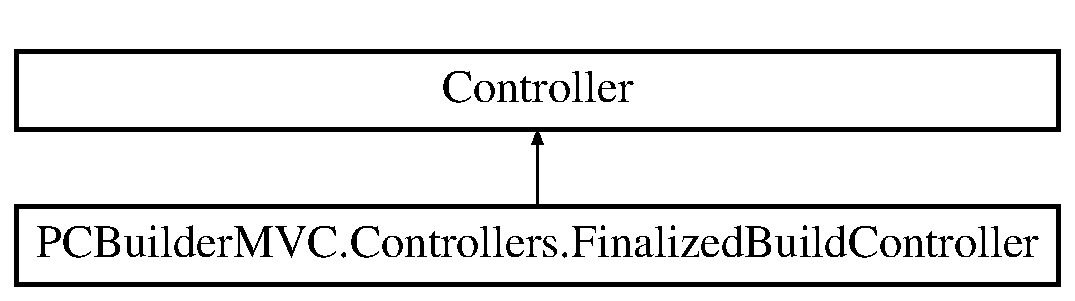
\includegraphics[height=2.000000cm]{class_p_c_builder_m_v_c_1_1_controllers_1_1_finalized_build_controller}
\end{center}
\end{figure}
\subsection*{Public Member Functions}
\begin{DoxyCompactItemize}
\item 
Action\+Result {\bfseries Index} ()\hypertarget{class_p_c_builder_m_v_c_1_1_controllers_1_1_finalized_build_controller_a242b5e426f4bc1c73fe627d400281f9e}{}\label{class_p_c_builder_m_v_c_1_1_controllers_1_1_finalized_build_controller_a242b5e426f4bc1c73fe627d400281f9e}

\item 
Action\+Result {\bfseries Details} (int?id)\hypertarget{class_p_c_builder_m_v_c_1_1_controllers_1_1_finalized_build_controller_a35dc61bcca940b614aab3c965bc0d2c9}{}\label{class_p_c_builder_m_v_c_1_1_controllers_1_1_finalized_build_controller_a35dc61bcca940b614aab3c965bc0d2c9}

\item 
Action\+Result {\bfseries Create} ()\hypertarget{class_p_c_builder_m_v_c_1_1_controllers_1_1_finalized_build_controller_a6bf70278e044bfd5e3f88ee514fb2249}{}\label{class_p_c_builder_m_v_c_1_1_controllers_1_1_finalized_build_controller_a6bf70278e044bfd5e3f88ee514fb2249}

\item 
Action\+Result {\bfseries Create} (\mbox{[}Bind(Include=\char`\"{}Finalized\+Build\+ID,message\char`\"{})\mbox{]} Finalized\+Build\+View\+Model finalized\+Build\+View\+Model)\hypertarget{class_p_c_builder_m_v_c_1_1_controllers_1_1_finalized_build_controller_ad7c02b253a9d65c0af1d2c8291bde7c7}{}\label{class_p_c_builder_m_v_c_1_1_controllers_1_1_finalized_build_controller_ad7c02b253a9d65c0af1d2c8291bde7c7}

\item 
Action\+Result {\bfseries Edit} (int?id)\hypertarget{class_p_c_builder_m_v_c_1_1_controllers_1_1_finalized_build_controller_a2060f2af464247f5856255019afd972c}{}\label{class_p_c_builder_m_v_c_1_1_controllers_1_1_finalized_build_controller_a2060f2af464247f5856255019afd972c}

\item 
Action\+Result {\bfseries Edit} (\mbox{[}Bind(Include=\char`\"{}Finalized\+Build\+ID,message\char`\"{})\mbox{]} Finalized\+Build\+View\+Model finalized\+Build\+View\+Model)\hypertarget{class_p_c_builder_m_v_c_1_1_controllers_1_1_finalized_build_controller_ab758e591d4fbd3f8735ff9b6d4b80974}{}\label{class_p_c_builder_m_v_c_1_1_controllers_1_1_finalized_build_controller_ab758e591d4fbd3f8735ff9b6d4b80974}

\item 
Action\+Result {\bfseries Delete} (int?id)\hypertarget{class_p_c_builder_m_v_c_1_1_controllers_1_1_finalized_build_controller_a67108920f596310eb9aee37122b5ccbe}{}\label{class_p_c_builder_m_v_c_1_1_controllers_1_1_finalized_build_controller_a67108920f596310eb9aee37122b5ccbe}

\item 
Action\+Result {\bfseries Delete\+Confirmed} (int id)\hypertarget{class_p_c_builder_m_v_c_1_1_controllers_1_1_finalized_build_controller_a1eafcada1b37f4df54b3a202209ee6ca}{}\label{class_p_c_builder_m_v_c_1_1_controllers_1_1_finalized_build_controller_a1eafcada1b37f4df54b3a202209ee6ca}

\end{DoxyCompactItemize}
\subsection*{Protected Member Functions}
\begin{DoxyCompactItemize}
\item 
override void {\bfseries Dispose} (bool disposing)\hypertarget{class_p_c_builder_m_v_c_1_1_controllers_1_1_finalized_build_controller_a5a502f607f19ae30e5b8b3c7b699a088}{}\label{class_p_c_builder_m_v_c_1_1_controllers_1_1_finalized_build_controller_a5a502f607f19ae30e5b8b3c7b699a088}

\end{DoxyCompactItemize}
\subsection*{Private Attributes}
\begin{DoxyCompactItemize}
\item 
\hyperlink{class_p_c_builder_m_v_c_1_1_models_1_1_p_c_builder_entity_models}{P\+C\+Builder\+Entity\+Models} {\bfseries db} = new \hyperlink{class_p_c_builder_m_v_c_1_1_models_1_1_p_c_builder_entity_models}{P\+C\+Builder\+Entity\+Models}()\hypertarget{class_p_c_builder_m_v_c_1_1_controllers_1_1_finalized_build_controller_ab36401b0c2a8a3eb9bf898d8123423cc}{}\label{class_p_c_builder_m_v_c_1_1_controllers_1_1_finalized_build_controller_ab36401b0c2a8a3eb9bf898d8123423cc}

\end{DoxyCompactItemize}


\subsection{Detailed Description}
Finalized build controller class to handle Finalized\+Build views interaction. 

\begin{DoxySeeAlso}{See also}
System.\+Web.\+Mvc.\+Controller


\end{DoxySeeAlso}


Definition at line 17 of file Finalized\+Build\+Controller.\+cs.



The documentation for this class was generated from the following file\+:\begin{DoxyCompactItemize}
\item 
C\+:/\+Users/nh228u08/\+Desktop/\+Final\+Project/\+Final\+Project/\+P\+C\+Builder/\+P\+C\+Builder\+M\+V\+C/\+Controllers/Finalized\+Build\+Controller.\+cs\end{DoxyCompactItemize}

\hypertarget{class_p_c_builder_m_v_c_1_1_models_1_1_finalized_build_view_model}{}\section{P\+C\+Builder\+M\+V\+C.\+Models.\+Finalized\+Build\+View\+Model Class Reference}
\label{class_p_c_builder_m_v_c_1_1_models_1_1_finalized_build_view_model}\index{P\+C\+Builder\+M\+V\+C.\+Models.\+Finalized\+Build\+View\+Model@{P\+C\+Builder\+M\+V\+C.\+Models.\+Finalized\+Build\+View\+Model}}


Finalized build view model class.  


\subsection*{Public Member Functions}
\begin{DoxyCompactItemize}
\item 
\hyperlink{class_p_c_builder_m_v_c_1_1_models_1_1_finalized_build_view_model_a2a66b39bc37ebd650493fa5a65c7994e}{Finalized\+Build\+View\+Model} (int id, \hyperlink{class_business_objects_1_1_finalized_build}{Business\+Objects.\+Finalized\+Build} fb)
\begin{DoxyCompactList}\small\item\em Initializes a new instance of the \hyperlink{class_p_c_builder_m_v_c_1_1_models_1_1_finalized_build_view_model}{Finalized\+Build\+View\+Model} class. \end{DoxyCompactList}\end{DoxyCompactItemize}
\subsection*{Properties}
\begin{DoxyCompactItemize}
\item 
int {\bfseries Finalized\+Build\+ID}\hspace{0.3cm}{\ttfamily  \mbox{[}get, set\mbox{]}}\hypertarget{class_p_c_builder_m_v_c_1_1_models_1_1_finalized_build_view_model_a1bbfda95f83c4234640986e9385b2af1}{}\label{class_p_c_builder_m_v_c_1_1_models_1_1_finalized_build_view_model_a1bbfda95f83c4234640986e9385b2af1}

\item 
\hyperlink{class_p_c_builder_m_v_c_1_1_models_1_1_c_p_u}{C\+PU} {\bfseries cpu}\hspace{0.3cm}{\ttfamily  \mbox{[}get, set\mbox{]}}\hypertarget{class_p_c_builder_m_v_c_1_1_models_1_1_finalized_build_view_model_aa7d884dfe24e6bc042f2c0553bfce985}{}\label{class_p_c_builder_m_v_c_1_1_models_1_1_finalized_build_view_model_aa7d884dfe24e6bc042f2c0553bfce985}

\item 
\hyperlink{class_p_c_builder_m_v_c_1_1_models_1_1_g_p_u}{G\+PU} {\bfseries gpu}\hspace{0.3cm}{\ttfamily  \mbox{[}get, set\mbox{]}}\hypertarget{class_p_c_builder_m_v_c_1_1_models_1_1_finalized_build_view_model_a46dbbfefa1922bf08858bd90d2041182}{}\label{class_p_c_builder_m_v_c_1_1_models_1_1_finalized_build_view_model_a46dbbfefa1922bf08858bd90d2041182}

\item 
\hyperlink{class_p_c_builder_m_v_c_1_1_models_1_1_motherboard}{Motherboard} {\bfseries motherboard}\hspace{0.3cm}{\ttfamily  \mbox{[}get, set\mbox{]}}\hypertarget{class_p_c_builder_m_v_c_1_1_models_1_1_finalized_build_view_model_aadf53b6998eb5d45cec159918cbd0705}{}\label{class_p_c_builder_m_v_c_1_1_models_1_1_finalized_build_view_model_aadf53b6998eb5d45cec159918cbd0705}

\item 
\hyperlink{class_p_c_builder_m_v_c_1_1_models_1_1_optical}{Optical} {\bfseries optical}\hspace{0.3cm}{\ttfamily  \mbox{[}get, set\mbox{]}}\hypertarget{class_p_c_builder_m_v_c_1_1_models_1_1_finalized_build_view_model_a1fde0b21cb9456e461b278732c4c22f3}{}\label{class_p_c_builder_m_v_c_1_1_models_1_1_finalized_build_view_model_a1fde0b21cb9456e461b278732c4c22f3}

\item 
\hyperlink{class_p_c_builder_m_v_c_1_1_models_1_1_p_s_u}{P\+SU} {\bfseries psu}\hspace{0.3cm}{\ttfamily  \mbox{[}get, set\mbox{]}}\hypertarget{class_p_c_builder_m_v_c_1_1_models_1_1_finalized_build_view_model_a75590a3997c9cfee09a320d021c89602}{}\label{class_p_c_builder_m_v_c_1_1_models_1_1_finalized_build_view_model_a75590a3997c9cfee09a320d021c89602}

\item 
\hyperlink{class_p_c_builder_m_v_c_1_1_models_1_1_r_a_m}{R\+AM} {\bfseries ram}\hspace{0.3cm}{\ttfamily  \mbox{[}get, set\mbox{]}}\hypertarget{class_p_c_builder_m_v_c_1_1_models_1_1_finalized_build_view_model_acebfbdfe40d252640101bcdc347f778c}{}\label{class_p_c_builder_m_v_c_1_1_models_1_1_finalized_build_view_model_acebfbdfe40d252640101bcdc347f778c}

\item 
\hyperlink{class_p_c_builder_m_v_c_1_1_models_1_1_storage}{Storage} {\bfseries storage}\hspace{0.3cm}{\ttfamily  \mbox{[}get, set\mbox{]}}\hypertarget{class_p_c_builder_m_v_c_1_1_models_1_1_finalized_build_view_model_af69a3753363097ef99289069b4c3f76d}{}\label{class_p_c_builder_m_v_c_1_1_models_1_1_finalized_build_view_model_af69a3753363097ef99289069b4c3f76d}

\item 
string {\bfseries message}\hspace{0.3cm}{\ttfamily  \mbox{[}get, set\mbox{]}}\hypertarget{class_p_c_builder_m_v_c_1_1_models_1_1_finalized_build_view_model_a0b9be8e5c91c6c0203d20cb0a5e0e5e9}{}\label{class_p_c_builder_m_v_c_1_1_models_1_1_finalized_build_view_model_a0b9be8e5c91c6c0203d20cb0a5e0e5e9}

\item 
decimal {\bfseries price}\hspace{0.3cm}{\ttfamily  \mbox{[}get, set\mbox{]}}\hypertarget{class_p_c_builder_m_v_c_1_1_models_1_1_finalized_build_view_model_aeac1173b02c5fde051f6902931b98635}{}\label{class_p_c_builder_m_v_c_1_1_models_1_1_finalized_build_view_model_aeac1173b02c5fde051f6902931b98635}

\end{DoxyCompactItemize}


\subsection{Detailed Description}
Finalized build view model class. 



Definition at line 12 of file Finalized\+Build\+View\+Model.\+cs.



\subsection{Constructor \& Destructor Documentation}
\index{P\+C\+Builder\+M\+V\+C\+::\+Models\+::\+Finalized\+Build\+View\+Model@{P\+C\+Builder\+M\+V\+C\+::\+Models\+::\+Finalized\+Build\+View\+Model}!Finalized\+Build\+View\+Model@{Finalized\+Build\+View\+Model}}
\index{Finalized\+Build\+View\+Model@{Finalized\+Build\+View\+Model}!P\+C\+Builder\+M\+V\+C\+::\+Models\+::\+Finalized\+Build\+View\+Model@{P\+C\+Builder\+M\+V\+C\+::\+Models\+::\+Finalized\+Build\+View\+Model}}
\subsubsection[{\texorpdfstring{Finalized\+Build\+View\+Model(int id, Business\+Objects.\+Finalized\+Build fb)}{FinalizedBuildViewModel(int id, BusinessObjects.FinalizedBuild fb)}}]{\setlength{\rightskip}{0pt plus 5cm}P\+C\+Builder\+M\+V\+C.\+Models.\+Finalized\+Build\+View\+Model.\+Finalized\+Build\+View\+Model (
\begin{DoxyParamCaption}
\item[{int}]{id, }
\item[{{\bf Business\+Objects.\+Finalized\+Build}}]{fb}
\end{DoxyParamCaption}
)}\hypertarget{class_p_c_builder_m_v_c_1_1_models_1_1_finalized_build_view_model_a2a66b39bc37ebd650493fa5a65c7994e}{}\label{class_p_c_builder_m_v_c_1_1_models_1_1_finalized_build_view_model_a2a66b39bc37ebd650493fa5a65c7994e}


Initializes a new instance of the \hyperlink{class_p_c_builder_m_v_c_1_1_models_1_1_finalized_build_view_model}{Finalized\+Build\+View\+Model} class. 


\begin{DoxyParams}{Parameters}
{\em id} & The identifier.\\
\hline
{\em fb} & The fb.\\
\hline
\end{DoxyParams}


This constructor serves the purpose of casting Finalized\+Build to \hyperlink{class_p_c_builder_m_v_c_1_1_models_1_1_finalized_build_view_model}{Finalized\+Build\+View\+Model} 

Definition at line 34 of file Finalized\+Build\+View\+Model.\+cs.



The documentation for this class was generated from the following file\+:\begin{DoxyCompactItemize}
\item 
C\+:/\+Users/nh228u08/\+Desktop/\+Final\+Project/\+Final\+Project/\+P\+C\+Builder/\+P\+C\+Builder\+M\+V\+C/\+Models/Finalized\+Build\+View\+Model.\+cs\end{DoxyCompactItemize}

\hypertarget{class_p_c_builder_m_v_c_1_1_models_1_1_forgot_password_view_model}{}\section{P\+C\+Builder\+M\+V\+C.\+Models.\+Forgot\+Password\+View\+Model Class Reference}
\label{class_p_c_builder_m_v_c_1_1_models_1_1_forgot_password_view_model}\index{P\+C\+Builder\+M\+V\+C.\+Models.\+Forgot\+Password\+View\+Model@{P\+C\+Builder\+M\+V\+C.\+Models.\+Forgot\+Password\+View\+Model}}


Forgot password view model class.  


\subsection*{Properties}
\begin{DoxyCompactItemize}
\item 
string {\bfseries Email}\hspace{0.3cm}{\ttfamily  \mbox{[}get, set\mbox{]}}\hypertarget{class_p_c_builder_m_v_c_1_1_models_1_1_forgot_password_view_model_a89b2c27d3ea7fc49e1edf10c801a09d4}{}\label{class_p_c_builder_m_v_c_1_1_models_1_1_forgot_password_view_model_a89b2c27d3ea7fc49e1edf10c801a09d4}

\end{DoxyCompactItemize}


\subsection{Detailed Description}
Forgot password view model class. 



Definition at line 115 of file Account\+View\+Models.\+cs.



The documentation for this class was generated from the following file\+:\begin{DoxyCompactItemize}
\item 
C\+:/\+Users/nh228u08/\+Desktop/\+Final\+Project/\+Final\+Project/\+P\+C\+Builder/\+P\+C\+Builder\+M\+V\+C/\+Models/Account\+View\+Models.\+cs\end{DoxyCompactItemize}

\hypertarget{class_p_c_builder_m_v_c_1_1_models_1_1_g_p_u}{}\section{P\+C\+Builder\+M\+V\+C.\+Models.\+G\+PU Class Reference}
\label{class_p_c_builder_m_v_c_1_1_models_1_1_g_p_u}\index{P\+C\+Builder\+M\+V\+C.\+Models.\+G\+PU@{P\+C\+Builder\+M\+V\+C.\+Models.\+G\+PU}}


\hyperlink{class_p_c_builder_m_v_c_1_1_models_1_1_g_p_u}{G\+PU} view model class.  


\subsection*{Properties}
\begin{DoxyCompactItemize}
\item 
int {\bfseries Gpu\+Id}\hspace{0.3cm}{\ttfamily  \mbox{[}get, set\mbox{]}}\hypertarget{class_p_c_builder_m_v_c_1_1_models_1_1_g_p_u_a94f2a1bac2d93ecbbeb724da3a08755b}{}\label{class_p_c_builder_m_v_c_1_1_models_1_1_g_p_u_a94f2a1bac2d93ecbbeb724da3a08755b}

\item 
string {\bfseries Brand}\hspace{0.3cm}{\ttfamily  \mbox{[}get, set\mbox{]}}\hypertarget{class_p_c_builder_m_v_c_1_1_models_1_1_g_p_u_a8afab1e0fe83bfe730cffbe144d11a09}{}\label{class_p_c_builder_m_v_c_1_1_models_1_1_g_p_u_a8afab1e0fe83bfe730cffbe144d11a09}

\item 
string {\bfseries Model}\hspace{0.3cm}{\ttfamily  \mbox{[}get, set\mbox{]}}\hypertarget{class_p_c_builder_m_v_c_1_1_models_1_1_g_p_u_a315da092d9c9524158f89139ce027152}{}\label{class_p_c_builder_m_v_c_1_1_models_1_1_g_p_u_a315da092d9c9524158f89139ce027152}

\item 
double {\bfseries Clock\+Speed}\hspace{0.3cm}{\ttfamily  \mbox{[}get, set\mbox{]}}\hypertarget{class_p_c_builder_m_v_c_1_1_models_1_1_g_p_u_acfe3c728a749c0433530e2667ab2fdd4}{}\label{class_p_c_builder_m_v_c_1_1_models_1_1_g_p_u_acfe3c728a749c0433530e2667ab2fdd4}

\item 
string {\bfseries Product\+Line\+Name}\hspace{0.3cm}{\ttfamily  \mbox{[}get, set\mbox{]}}\hypertarget{class_p_c_builder_m_v_c_1_1_models_1_1_g_p_u_a8d5a1828631eda6bef943c87646564fd}{}\label{class_p_c_builder_m_v_c_1_1_models_1_1_g_p_u_a8d5a1828631eda6bef943c87646564fd}

\item 
int {\bfseries Benchmark\+Score}\hspace{0.3cm}{\ttfamily  \mbox{[}get, set\mbox{]}}\hypertarget{class_p_c_builder_m_v_c_1_1_models_1_1_g_p_u_aa72a1ca6f5e1490774b766c8c9cc9801}{}\label{class_p_c_builder_m_v_c_1_1_models_1_1_g_p_u_aa72a1ca6f5e1490774b766c8c9cc9801}

\item 
string {\bfseries Best\+Use}\hspace{0.3cm}{\ttfamily  \mbox{[}get, set\mbox{]}}\hypertarget{class_p_c_builder_m_v_c_1_1_models_1_1_g_p_u_a9de5246b116d06d7783ef5e06e2d8cc0}{}\label{class_p_c_builder_m_v_c_1_1_models_1_1_g_p_u_a9de5246b116d06d7783ef5e06e2d8cc0}

\item 
int {\bfseries Gpu\+Ram\+Size}\hspace{0.3cm}{\ttfamily  \mbox{[}get, set\mbox{]}}\hypertarget{class_p_c_builder_m_v_c_1_1_models_1_1_g_p_u_a15f0b0b6bcdcdcda0541944b331cbf92}{}\label{class_p_c_builder_m_v_c_1_1_models_1_1_g_p_u_a15f0b0b6bcdcdcda0541944b331cbf92}

\item 
int {\bfseries Pci\+Pin\+Connector1}\hspace{0.3cm}{\ttfamily  \mbox{[}get, set\mbox{]}}\hypertarget{class_p_c_builder_m_v_c_1_1_models_1_1_g_p_u_aa3948c4837e919bd13b83c17a5e0a221}{}\label{class_p_c_builder_m_v_c_1_1_models_1_1_g_p_u_aa3948c4837e919bd13b83c17a5e0a221}

\item 
int {\bfseries Pci\+Pin\+Connector2}\hspace{0.3cm}{\ttfamily  \mbox{[}get, set\mbox{]}}\hypertarget{class_p_c_builder_m_v_c_1_1_models_1_1_g_p_u_ab4cd6e4b85bd065395392d870043235d}{}\label{class_p_c_builder_m_v_c_1_1_models_1_1_g_p_u_ab4cd6e4b85bd065395392d870043235d}

\item 
int {\bfseries Pci\+Pin\+Connector3}\hspace{0.3cm}{\ttfamily  \mbox{[}get, set\mbox{]}}\hypertarget{class_p_c_builder_m_v_c_1_1_models_1_1_g_p_u_ababb8f55a980a75c24e3f0a3eddb3049}{}\label{class_p_c_builder_m_v_c_1_1_models_1_1_g_p_u_ababb8f55a980a75c24e3f0a3eddb3049}

\item 
int {\bfseries Power\+Requirement}\hspace{0.3cm}{\ttfamily  \mbox{[}get, set\mbox{]}}\hypertarget{class_p_c_builder_m_v_c_1_1_models_1_1_g_p_u_a333b107c1d0bf013dc42a41d86033f7f}{}\label{class_p_c_builder_m_v_c_1_1_models_1_1_g_p_u_a333b107c1d0bf013dc42a41d86033f7f}

\item 
string {\bfseries Gpu\+Length}\hspace{0.3cm}{\ttfamily  \mbox{[}get, set\mbox{]}}\hypertarget{class_p_c_builder_m_v_c_1_1_models_1_1_g_p_u_a584361d4507698bc9cb51fee3154102d}{}\label{class_p_c_builder_m_v_c_1_1_models_1_1_g_p_u_a584361d4507698bc9cb51fee3154102d}

\item 
decimal {\bfseries Price}\hspace{0.3cm}{\ttfamily  \mbox{[}get, set\mbox{]}}\hypertarget{class_p_c_builder_m_v_c_1_1_models_1_1_g_p_u_ac3a4b525102cbae0f080ce1afae79c7f}{}\label{class_p_c_builder_m_v_c_1_1_models_1_1_g_p_u_ac3a4b525102cbae0f080ce1afae79c7f}

\end{DoxyCompactItemize}


\subsection{Detailed Description}
\hyperlink{class_p_c_builder_m_v_c_1_1_models_1_1_g_p_u}{G\+PU} view model class. 



Definition at line 13 of file G\+P\+U.\+cs.



The documentation for this class was generated from the following file\+:\begin{DoxyCompactItemize}
\item 
C\+:/\+Users/nh228u08/\+Desktop/\+Final\+Project/\+Final\+Project/\+P\+C\+Builder/\+P\+C\+Builder\+M\+V\+C/\+Models/G\+P\+U.\+cs\end{DoxyCompactItemize}

\hypertarget{class_business_objects_1_1_g_p_u}{}\section{Business\+Objects.\+G\+PU Class Reference}
\label{class_business_objects_1_1_g_p_u}\index{Business\+Objects.\+G\+PU@{Business\+Objects.\+G\+PU}}


\hyperlink{class_business_objects_1_1_g_p_u}{G\+PU} object to hold necessary data on the \hyperlink{class_business_objects_1_1_g_p_u}{G\+PU}.  


\subsection*{Public Member Functions}
\begin{DoxyCompactItemize}
\item 
\hyperlink{class_business_objects_1_1_g_p_u_ab773228207f38d564b424c819a4fc9c8}{G\+PU} ()
\begin{DoxyCompactList}\small\item\em Initializes a new instance of the \hyperlink{class_business_objects_1_1_g_p_u}{G\+PU} class. \end{DoxyCompactList}\item 
\hyperlink{class_business_objects_1_1_g_p_u_a444248551f8e905f4e5cbfa1e6f9b90a}{G\+PU} (int gpu\+Id, string brand, string model, double clock\+Speed, string product\+Line\+Name, int benchmark\+Score, string best\+Use, int gpu\+Ram\+Size, int pci\+Pin\+Connector1, int pci\+Pin\+Connector2, int pci\+Pin\+Connector3, int power\+Requirement, char gpu\+Length, decimal price)
\begin{DoxyCompactList}\small\item\em Initializes a new instance of the \hyperlink{class_business_objects_1_1_g_p_u}{G\+PU} class. \end{DoxyCompactList}\end{DoxyCompactItemize}
\subsection*{Properties}
\begin{DoxyCompactItemize}
\item 
int {\bfseries Gpu\+Id}\hspace{0.3cm}{\ttfamily  \mbox{[}get, set\mbox{]}}\hypertarget{class_business_objects_1_1_g_p_u_afeb1e8b9b58e0400721046e676cc3614}{}\label{class_business_objects_1_1_g_p_u_afeb1e8b9b58e0400721046e676cc3614}

\item 
string {\bfseries Brand}\hspace{0.3cm}{\ttfamily  \mbox{[}get, set\mbox{]}}\hypertarget{class_business_objects_1_1_g_p_u_af2f55e8a9725448cead02124bbab762d}{}\label{class_business_objects_1_1_g_p_u_af2f55e8a9725448cead02124bbab762d}

\item 
string {\bfseries Model}\hspace{0.3cm}{\ttfamily  \mbox{[}get, set\mbox{]}}\hypertarget{class_business_objects_1_1_g_p_u_aa9e024751d02378f97e24e80cb8dfc22}{}\label{class_business_objects_1_1_g_p_u_aa9e024751d02378f97e24e80cb8dfc22}

\item 
double {\bfseries Clock\+Speed}\hspace{0.3cm}{\ttfamily  \mbox{[}get, set\mbox{]}}\hypertarget{class_business_objects_1_1_g_p_u_a1b68b71a45aad6cdea19b43d6043c69b}{}\label{class_business_objects_1_1_g_p_u_a1b68b71a45aad6cdea19b43d6043c69b}

\item 
string {\bfseries Product\+Line\+Name}\hspace{0.3cm}{\ttfamily  \mbox{[}get, set\mbox{]}}\hypertarget{class_business_objects_1_1_g_p_u_a30166940091fc02016e2c16b942b8f81}{}\label{class_business_objects_1_1_g_p_u_a30166940091fc02016e2c16b942b8f81}

\item 
int {\bfseries Benchmark\+Score}\hspace{0.3cm}{\ttfamily  \mbox{[}get, set\mbox{]}}\hypertarget{class_business_objects_1_1_g_p_u_a5e71ca43b91549127e3303966f9c1883}{}\label{class_business_objects_1_1_g_p_u_a5e71ca43b91549127e3303966f9c1883}

\item 
string {\bfseries Best\+Use}\hspace{0.3cm}{\ttfamily  \mbox{[}get, set\mbox{]}}\hypertarget{class_business_objects_1_1_g_p_u_a8cb10d609af32f50b4efaa38fcff82da}{}\label{class_business_objects_1_1_g_p_u_a8cb10d609af32f50b4efaa38fcff82da}

\item 
int {\bfseries Gpu\+Ram\+Size}\hspace{0.3cm}{\ttfamily  \mbox{[}get, set\mbox{]}}\hypertarget{class_business_objects_1_1_g_p_u_ab38f21d1da4e4b6d16bc00e1a3077c38}{}\label{class_business_objects_1_1_g_p_u_ab38f21d1da4e4b6d16bc00e1a3077c38}

\item 
int {\bfseries Pci\+Pin\+Connector1}\hspace{0.3cm}{\ttfamily  \mbox{[}get, set\mbox{]}}\hypertarget{class_business_objects_1_1_g_p_u_a2d08d354f962c6c77cd9e29e623f776f}{}\label{class_business_objects_1_1_g_p_u_a2d08d354f962c6c77cd9e29e623f776f}

\item 
int {\bfseries Pci\+Pin\+Connector2}\hspace{0.3cm}{\ttfamily  \mbox{[}get, set\mbox{]}}\hypertarget{class_business_objects_1_1_g_p_u_a29b8be931b594510733fb12ebafda81b}{}\label{class_business_objects_1_1_g_p_u_a29b8be931b594510733fb12ebafda81b}

\item 
int {\bfseries Pci\+Pin\+Connector3}\hspace{0.3cm}{\ttfamily  \mbox{[}get, set\mbox{]}}\hypertarget{class_business_objects_1_1_g_p_u_a3c73e1c2905ca5c93207dc84537c71bc}{}\label{class_business_objects_1_1_g_p_u_a3c73e1c2905ca5c93207dc84537c71bc}

\item 
int {\bfseries Power\+Requirement}\hspace{0.3cm}{\ttfamily  \mbox{[}get, set\mbox{]}}\hypertarget{class_business_objects_1_1_g_p_u_a28e5f1a2955634bdb563d5ae5904d9ce}{}\label{class_business_objects_1_1_g_p_u_a28e5f1a2955634bdb563d5ae5904d9ce}

\item 
char {\bfseries Gpu\+Length}\hspace{0.3cm}{\ttfamily  \mbox{[}get, set\mbox{]}}\hypertarget{class_business_objects_1_1_g_p_u_ab5a737850479b96f7530d4c852acc4b8}{}\label{class_business_objects_1_1_g_p_u_ab5a737850479b96f7530d4c852acc4b8}

\item 
decimal {\bfseries Price}\hspace{0.3cm}{\ttfamily  \mbox{[}get, set\mbox{]}}\hypertarget{class_business_objects_1_1_g_p_u_a2640d3a1607005bb9c89a39218aa3e39}{}\label{class_business_objects_1_1_g_p_u_a2640d3a1607005bb9c89a39218aa3e39}

\end{DoxyCompactItemize}


\subsection{Detailed Description}
\hyperlink{class_business_objects_1_1_g_p_u}{G\+PU} object to hold necessary data on the \hyperlink{class_business_objects_1_1_g_p_u}{G\+PU}. 



Definition at line 17 of file G\+P\+U.\+cs.



\subsection{Constructor \& Destructor Documentation}
\index{Business\+Objects\+::\+G\+PU@{Business\+Objects\+::\+G\+PU}!G\+PU@{G\+PU}}
\index{G\+PU@{G\+PU}!Business\+Objects\+::\+G\+PU@{Business\+Objects\+::\+G\+PU}}
\subsubsection[{\texorpdfstring{G\+P\+U()}{GPU()}}]{\setlength{\rightskip}{0pt plus 5cm}Business\+Objects.\+G\+P\+U.\+G\+PU (
\begin{DoxyParamCaption}
{}
\end{DoxyParamCaption}
)}\hypertarget{class_business_objects_1_1_g_p_u_ab773228207f38d564b424c819a4fc9c8}{}\label{class_business_objects_1_1_g_p_u_ab773228207f38d564b424c819a4fc9c8}


Initializes a new instance of the \hyperlink{class_business_objects_1_1_g_p_u}{G\+PU} class. 



Definition at line 37 of file G\+P\+U.\+cs.

\index{Business\+Objects\+::\+G\+PU@{Business\+Objects\+::\+G\+PU}!G\+PU@{G\+PU}}
\index{G\+PU@{G\+PU}!Business\+Objects\+::\+G\+PU@{Business\+Objects\+::\+G\+PU}}
\subsubsection[{\texorpdfstring{G\+P\+U(int gpu\+Id, string brand, string model, double clock\+Speed, string product\+Line\+Name, int benchmark\+Score, string best\+Use, int gpu\+Ram\+Size, int pci\+Pin\+Connector1, int pci\+Pin\+Connector2, int pci\+Pin\+Connector3, int power\+Requirement, char gpu\+Length, decimal price)}{GPU(int gpuId, string brand, string model, double clockSpeed, string productLineName, int benchmarkScore, string bestUse, int gpuRamSize, int pciPinConnector1, int pciPinConnector2, int pciPinConnector3, int powerRequirement, char gpuLength, decimal price)}}]{\setlength{\rightskip}{0pt plus 5cm}Business\+Objects.\+G\+P\+U.\+G\+PU (
\begin{DoxyParamCaption}
\item[{int}]{gpu\+Id, }
\item[{string}]{brand, }
\item[{string}]{model, }
\item[{double}]{clock\+Speed, }
\item[{string}]{product\+Line\+Name, }
\item[{int}]{benchmark\+Score, }
\item[{string}]{best\+Use, }
\item[{int}]{gpu\+Ram\+Size, }
\item[{int}]{pci\+Pin\+Connector1, }
\item[{int}]{pci\+Pin\+Connector2, }
\item[{int}]{pci\+Pin\+Connector3, }
\item[{int}]{power\+Requirement, }
\item[{char}]{gpu\+Length, }
\item[{decimal}]{price}
\end{DoxyParamCaption}
)}\hypertarget{class_business_objects_1_1_g_p_u_a444248551f8e905f4e5cbfa1e6f9b90a}{}\label{class_business_objects_1_1_g_p_u_a444248551f8e905f4e5cbfa1e6f9b90a}


Initializes a new instance of the \hyperlink{class_business_objects_1_1_g_p_u}{G\+PU} class. 


\begin{DoxyParams}{Parameters}
{\em gpu\+Id} & The \hyperlink{class_business_objects_1_1_g_p_u}{G\+PU} identifier.\\
\hline
{\em brand} & The brand.\\
\hline
{\em model} & The model.\\
\hline
{\em clock\+Speed} & The clock speed.\\
\hline
{\em product\+Line\+Name} & Name of the product line.\\
\hline
{\em benchmark\+Score} & The benchmark score.\\
\hline
{\em best\+Use} & The best use case.\\
\hline
{\em gpu\+Ram\+Size} & Size of the \hyperlink{class_business_objects_1_1_g_p_u}{G\+PU} ram.\\
\hline
{\em pci\+Pin\+Connector1} & The P\+C\+Ie pin connector \#1.\\
\hline
{\em pci\+Pin\+Connector2} & The P\+C\+Ie pin connector \#2.\\
\hline
{\em pci\+Pin\+Connector3} & The P\+C\+Ie pin connector \#3.\\
\hline
{\em power\+Requirement} & The power requirement.\\
\hline
{\em gpu\+Length} & Length of the \hyperlink{class_business_objects_1_1_g_p_u}{G\+PU}.\\
\hline
{\em price} & The price.\\
\hline
\end{DoxyParams}


Definition at line 56 of file G\+P\+U.\+cs.



The documentation for this class was generated from the following file\+:\begin{DoxyCompactItemize}
\item 
C\+:/\+Users/nh228u08/\+Desktop/\+Final\+Project/\+Final\+Project/\+P\+C\+Builder/\+Business\+Objects/G\+P\+U.\+cs\end{DoxyCompactItemize}

\hypertarget{class_data_access_1_1_g_p_u_accessor}{}\section{Data\+Access.\+G\+P\+U\+Accessor Class Reference}
\label{class_data_access_1_1_g_p_u_accessor}\index{Data\+Access.\+G\+P\+U\+Accessor@{Data\+Access.\+G\+P\+U\+Accessor}}


G\+PU accessor to communicate with database on G\+PU objects.  


\subsection*{Static Public Member Functions}
\begin{DoxyCompactItemize}
\item 
static \hyperlink{class_business_objects_1_1_g_p_u}{G\+PU} \hyperlink{class_data_access_1_1_g_p_u_accessor_acd3cccc36aed6c7c9fd3af8077fb3ec7}{Retrieve\+G\+P\+U\+By\+Name} (string name)
\begin{DoxyCompactList}\small\item\em Retrieves a G\+PU by name. \end{DoxyCompactList}\item 
static List$<$ \hyperlink{class_business_objects_1_1_g_p_u}{G\+PU} $>$ \hyperlink{class_data_access_1_1_g_p_u_accessor_a7203a061e7e659546c2c0240944c595b}{Retrieve\+G\+P\+Us\+By\+Ram\+Size} (int ram\+Size)
\begin{DoxyCompactList}\small\item\em Retrieves lsit of G\+P\+Us by R\+AM size. \end{DoxyCompactList}\item 
static int \hyperlink{class_data_access_1_1_g_p_u_accessor_a7fba4be184695de0c77385bc74ee50f0}{Insert\+Gpu} (\hyperlink{class_business_objects_1_1_g_p_u}{G\+PU} gpu)
\begin{DoxyCompactList}\small\item\em Inserts a new G\+PU. \end{DoxyCompactList}\item 
static List$<$ \hyperlink{class_business_objects_1_1_g_p_u}{G\+PU} $>$ \hyperlink{class_data_access_1_1_g_p_u_accessor_ad0e40a593f48af857d32b9386ee02cd6}{Retrieve\+All\+G\+PU} ()
\begin{DoxyCompactList}\small\item\em Retrieves all G\+P\+Us. \end{DoxyCompactList}\end{DoxyCompactItemize}


\subsection{Detailed Description}
G\+PU accessor to communicate with database on G\+PU objects. 



Definition at line 15 of file G\+P\+U\+Accessor.\+cs.



\subsection{Member Function Documentation}
\index{Data\+Access\+::\+G\+P\+U\+Accessor@{Data\+Access\+::\+G\+P\+U\+Accessor}!Insert\+Gpu@{Insert\+Gpu}}
\index{Insert\+Gpu@{Insert\+Gpu}!Data\+Access\+::\+G\+P\+U\+Accessor@{Data\+Access\+::\+G\+P\+U\+Accessor}}
\subsubsection[{\texorpdfstring{Insert\+Gpu(\+G\+P\+U gpu)}{InsertGpu(GPU gpu)}}]{\setlength{\rightskip}{0pt plus 5cm}static int Data\+Access.\+G\+P\+U\+Accessor.\+Insert\+Gpu (
\begin{DoxyParamCaption}
\item[{{\bf G\+PU}}]{gpu}
\end{DoxyParamCaption}
)\hspace{0.3cm}{\ttfamily [static]}}\hypertarget{class_data_access_1_1_g_p_u_accessor_a7fba4be184695de0c77385bc74ee50f0}{}\label{class_data_access_1_1_g_p_u_accessor_a7fba4be184695de0c77385bc74ee50f0}


Inserts a new G\+PU. 


\begin{DoxyParams}{Parameters}
{\em gpu} & The gpu.\\
\hline
\end{DoxyParams}
\begin{DoxyReturn}{Returns}
Count of rows affected.
\end{DoxyReturn}


Definition at line 139 of file G\+P\+U\+Accessor.\+cs.

\index{Data\+Access\+::\+G\+P\+U\+Accessor@{Data\+Access\+::\+G\+P\+U\+Accessor}!Retrieve\+All\+G\+PU@{Retrieve\+All\+G\+PU}}
\index{Retrieve\+All\+G\+PU@{Retrieve\+All\+G\+PU}!Data\+Access\+::\+G\+P\+U\+Accessor@{Data\+Access\+::\+G\+P\+U\+Accessor}}
\subsubsection[{\texorpdfstring{Retrieve\+All\+G\+P\+U()}{RetrieveAllGPU()}}]{\setlength{\rightskip}{0pt plus 5cm}static List$<${\bf G\+PU}$>$ Data\+Access.\+G\+P\+U\+Accessor.\+Retrieve\+All\+G\+PU (
\begin{DoxyParamCaption}
{}
\end{DoxyParamCaption}
)\hspace{0.3cm}{\ttfamily [static]}}\hypertarget{class_data_access_1_1_g_p_u_accessor_ad0e40a593f48af857d32b9386ee02cd6}{}\label{class_data_access_1_1_g_p_u_accessor_ad0e40a593f48af857d32b9386ee02cd6}


Retrieves all G\+P\+Us. 

\begin{DoxyReturn}{Returns}
List of G\+PU objects.
\end{DoxyReturn}

\begin{DoxyExceptions}{Exceptions}
{\em System.\+Application\+Exception} & Data not found.\\
\hline
\end{DoxyExceptions}


Definition at line 185 of file G\+P\+U\+Accessor.\+cs.

\index{Data\+Access\+::\+G\+P\+U\+Accessor@{Data\+Access\+::\+G\+P\+U\+Accessor}!Retrieve\+G\+P\+U\+By\+Name@{Retrieve\+G\+P\+U\+By\+Name}}
\index{Retrieve\+G\+P\+U\+By\+Name@{Retrieve\+G\+P\+U\+By\+Name}!Data\+Access\+::\+G\+P\+U\+Accessor@{Data\+Access\+::\+G\+P\+U\+Accessor}}
\subsubsection[{\texorpdfstring{Retrieve\+G\+P\+U\+By\+Name(string name)}{RetrieveGPUByName(string name)}}]{\setlength{\rightskip}{0pt plus 5cm}static {\bf G\+PU} Data\+Access.\+G\+P\+U\+Accessor.\+Retrieve\+G\+P\+U\+By\+Name (
\begin{DoxyParamCaption}
\item[{string}]{name}
\end{DoxyParamCaption}
)\hspace{0.3cm}{\ttfamily [static]}}\hypertarget{class_data_access_1_1_g_p_u_accessor_acd3cccc36aed6c7c9fd3af8077fb3ec7}{}\label{class_data_access_1_1_g_p_u_accessor_acd3cccc36aed6c7c9fd3af8077fb3ec7}


Retrieves a G\+PU by name. 


\begin{DoxyParams}{Parameters}
{\em name} & The name.\\
\hline
\end{DoxyParams}
\begin{DoxyReturn}{Returns}
A G\+PU object.
\end{DoxyReturn}

\begin{DoxyExceptions}{Exceptions}
{\em System.\+Application\+Exception} & Data not found\\
\hline
\end{DoxyExceptions}


Definition at line 23 of file G\+P\+U\+Accessor.\+cs.

\index{Data\+Access\+::\+G\+P\+U\+Accessor@{Data\+Access\+::\+G\+P\+U\+Accessor}!Retrieve\+G\+P\+Us\+By\+Ram\+Size@{Retrieve\+G\+P\+Us\+By\+Ram\+Size}}
\index{Retrieve\+G\+P\+Us\+By\+Ram\+Size@{Retrieve\+G\+P\+Us\+By\+Ram\+Size}!Data\+Access\+::\+G\+P\+U\+Accessor@{Data\+Access\+::\+G\+P\+U\+Accessor}}
\subsubsection[{\texorpdfstring{Retrieve\+G\+P\+Us\+By\+Ram\+Size(int ram\+Size)}{RetrieveGPUsByRamSize(int ramSize)}}]{\setlength{\rightskip}{0pt plus 5cm}static List$<${\bf G\+PU}$>$ Data\+Access.\+G\+P\+U\+Accessor.\+Retrieve\+G\+P\+Us\+By\+Ram\+Size (
\begin{DoxyParamCaption}
\item[{int}]{ram\+Size}
\end{DoxyParamCaption}
)\hspace{0.3cm}{\ttfamily [static]}}\hypertarget{class_data_access_1_1_g_p_u_accessor_a7203a061e7e659546c2c0240944c595b}{}\label{class_data_access_1_1_g_p_u_accessor_a7203a061e7e659546c2c0240944c595b}


Retrieves lsit of G\+P\+Us by R\+AM size. 


\begin{DoxyParams}{Parameters}
{\em ram\+Size} & Size of the ram.\\
\hline
\end{DoxyParams}
\begin{DoxyReturn}{Returns}
List of G\+PU objects.
\end{DoxyReturn}

\begin{DoxyExceptions}{Exceptions}
{\em System.\+Application\+Exception} & Data not found\\
\hline
\end{DoxyExceptions}


Definition at line 81 of file G\+P\+U\+Accessor.\+cs.



The documentation for this class was generated from the following file\+:\begin{DoxyCompactItemize}
\item 
C\+:/\+Users/nh228u08/\+Desktop/\+Final\+Project/\+Final\+Project/\+P\+C\+Builder/\+Data\+Access/G\+P\+U\+Accessor.\+cs\end{DoxyCompactItemize}

\hypertarget{class_p_c_builder_m_v_c_1_1_controllers_1_1_g_p_u_controller}{}\section{P\+C\+Builder\+M\+V\+C.\+Controllers.\+G\+P\+U\+Controller Class Reference}
\label{class_p_c_builder_m_v_c_1_1_controllers_1_1_g_p_u_controller}\index{P\+C\+Builder\+M\+V\+C.\+Controllers.\+G\+P\+U\+Controller@{P\+C\+Builder\+M\+V\+C.\+Controllers.\+G\+P\+U\+Controller}}


G\+PU controller class to handle G\+PU views interaction.  


Inheritance diagram for P\+C\+Builder\+M\+V\+C.\+Controllers.\+G\+P\+U\+Controller\+:\begin{figure}[H]
\begin{center}
\leavevmode
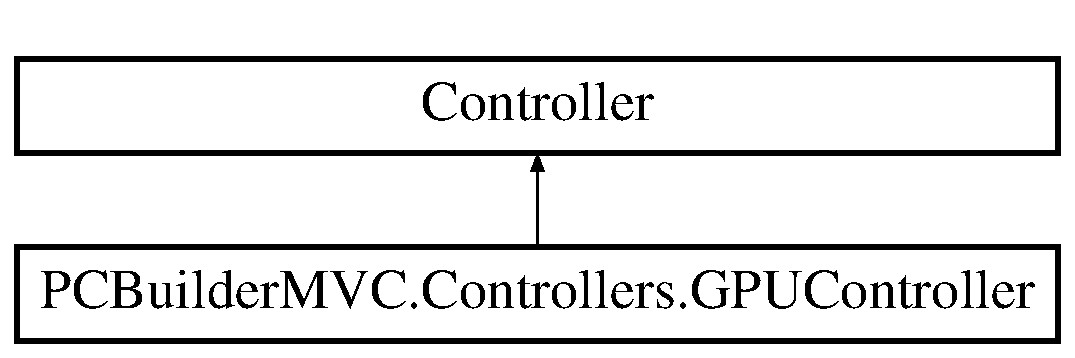
\includegraphics[height=2.000000cm]{class_p_c_builder_m_v_c_1_1_controllers_1_1_g_p_u_controller}
\end{center}
\end{figure}
\subsection*{Public Member Functions}
\begin{DoxyCompactItemize}
\item 
Action\+Result {\bfseries Index} ()\hypertarget{class_p_c_builder_m_v_c_1_1_controllers_1_1_g_p_u_controller_a38923ec0854ca8ca5d0247bae3068d4f}{}\label{class_p_c_builder_m_v_c_1_1_controllers_1_1_g_p_u_controller_a38923ec0854ca8ca5d0247bae3068d4f}

\item 
Action\+Result {\bfseries Details} (int?id)\hypertarget{class_p_c_builder_m_v_c_1_1_controllers_1_1_g_p_u_controller_a78d3d59dbfde397dbddb047d0c7db090}{}\label{class_p_c_builder_m_v_c_1_1_controllers_1_1_g_p_u_controller_a78d3d59dbfde397dbddb047d0c7db090}

\item 
Action\+Result {\bfseries Create} ()\hypertarget{class_p_c_builder_m_v_c_1_1_controllers_1_1_g_p_u_controller_ace84f79eaf685c05dce52af070c4b519}{}\label{class_p_c_builder_m_v_c_1_1_controllers_1_1_g_p_u_controller_ace84f79eaf685c05dce52af070c4b519}

\item 
Action\+Result {\bfseries Create} (\mbox{[}Bind(Include=\char`\"{}Gpu\+Id,Brand,Model,Clock\+Speed,Product\+Line\+Name,Benchmark\+Score,Best\+Use,Gpu\+Ram\+Size,Pci\+Pin\+Connector1,Pci\+Pin\+Connector2,Pci\+Pin\+Connector3,Power\+Requirement,Gpu\+Length,Price\char`\"{})\mbox{]} G\+PU g\+PU)\hypertarget{class_p_c_builder_m_v_c_1_1_controllers_1_1_g_p_u_controller_aa34201847e1e5c053d778e2b0a38650e}{}\label{class_p_c_builder_m_v_c_1_1_controllers_1_1_g_p_u_controller_aa34201847e1e5c053d778e2b0a38650e}

\item 
Action\+Result {\bfseries Edit} (int?id)\hypertarget{class_p_c_builder_m_v_c_1_1_controllers_1_1_g_p_u_controller_aeb7156b1f3d6bab93118cb778e75bea8}{}\label{class_p_c_builder_m_v_c_1_1_controllers_1_1_g_p_u_controller_aeb7156b1f3d6bab93118cb778e75bea8}

\item 
Action\+Result {\bfseries Edit} (\mbox{[}Bind(Include=\char`\"{}Gpu\+Id,Brand,Model,Clock\+Speed,Product\+Line\+Name,Benchmark\+Score,Best\+Use,Gpu\+Ram\+Size,Pci\+Pin\+Connector1,Pci\+Pin\+Connector2,Pci\+Pin\+Connector3,Power\+Requirement,Gpu\+Length,Price\char`\"{})\mbox{]} G\+PU g\+PU)\hypertarget{class_p_c_builder_m_v_c_1_1_controllers_1_1_g_p_u_controller_a0d21736b4431a17c038d500bf09ba00e}{}\label{class_p_c_builder_m_v_c_1_1_controllers_1_1_g_p_u_controller_a0d21736b4431a17c038d500bf09ba00e}

\item 
Action\+Result {\bfseries Delete} (int?id)\hypertarget{class_p_c_builder_m_v_c_1_1_controllers_1_1_g_p_u_controller_abf8b845362784a12062436f4720b14e6}{}\label{class_p_c_builder_m_v_c_1_1_controllers_1_1_g_p_u_controller_abf8b845362784a12062436f4720b14e6}

\item 
Action\+Result {\bfseries Delete\+Confirmed} (int id)\hypertarget{class_p_c_builder_m_v_c_1_1_controllers_1_1_g_p_u_controller_aab97b4bb193c7a42426beaa2c5ef2288}{}\label{class_p_c_builder_m_v_c_1_1_controllers_1_1_g_p_u_controller_aab97b4bb193c7a42426beaa2c5ef2288}

\end{DoxyCompactItemize}
\subsection*{Protected Member Functions}
\begin{DoxyCompactItemize}
\item 
override void {\bfseries Dispose} (bool disposing)\hypertarget{class_p_c_builder_m_v_c_1_1_controllers_1_1_g_p_u_controller_a034e1443604844a81742a6c4e2dd5ccf}{}\label{class_p_c_builder_m_v_c_1_1_controllers_1_1_g_p_u_controller_a034e1443604844a81742a6c4e2dd5ccf}

\end{DoxyCompactItemize}
\subsection*{Private Attributes}
\begin{DoxyCompactItemize}
\item 
\hyperlink{class_p_c_builder_m_v_c_1_1_models_1_1_p_c_builder_entity_models}{P\+C\+Builder\+Entity\+Models} {\bfseries db} = new \hyperlink{class_p_c_builder_m_v_c_1_1_models_1_1_p_c_builder_entity_models}{P\+C\+Builder\+Entity\+Models}()\hypertarget{class_p_c_builder_m_v_c_1_1_controllers_1_1_g_p_u_controller_a2d429161edc3b0d41d4b6ffedd323386}{}\label{class_p_c_builder_m_v_c_1_1_controllers_1_1_g_p_u_controller_a2d429161edc3b0d41d4b6ffedd323386}

\end{DoxyCompactItemize}


\subsection{Detailed Description}
G\+PU controller class to handle G\+PU views interaction. 

\begin{DoxySeeAlso}{See also}
System.\+Web.\+Mvc.\+Controller


\end{DoxySeeAlso}


Definition at line 17 of file G\+P\+U\+Controller.\+cs.



The documentation for this class was generated from the following file\+:\begin{DoxyCompactItemize}
\item 
C\+:/\+Users/nh228u08/\+Desktop/\+Final\+Project/\+Final\+Project/\+P\+C\+Builder/\+P\+C\+Builder\+M\+V\+C/\+Controllers/G\+P\+U\+Controller.\+cs\end{DoxyCompactItemize}

\hypertarget{class_business_logic_1_1_hash_methods}{}\section{Business\+Logic.\+Hash\+Methods Class Reference}
\label{class_business_logic_1_1_hash_methods}\index{Business\+Logic.\+Hash\+Methods@{Business\+Logic.\+Hash\+Methods}}


Hash method class containing the Sha256 hashing method.  


\subsection*{Static Public Member Functions}
\begin{DoxyCompactItemize}
\item 
static string \hyperlink{class_business_logic_1_1_hash_methods_a8d882378500b661e39d7201d2b89aed2}{Hash\+Sha256} (this string source)
\begin{DoxyCompactList}\small\item\em Hashes the passed value. \end{DoxyCompactList}\item 
static bool \hyperlink{class_business_logic_1_1_hash_methods_a921c0dc701d7a46d7cbdb36e0409f025}{Verify\+Sha256\+Hash} (this string compare\+String, string hash\+String)
\begin{DoxyCompactList}\small\item\em Verifies the sha256 hash. \end{DoxyCompactList}\end{DoxyCompactItemize}


\subsection{Detailed Description}
Hash method class containing the Sha256 hashing method. 



Definition at line 13 of file Hash\+Methods.\+cs.



\subsection{Member Function Documentation}
\index{Business\+Logic\+::\+Hash\+Methods@{Business\+Logic\+::\+Hash\+Methods}!Hash\+Sha256@{Hash\+Sha256}}
\index{Hash\+Sha256@{Hash\+Sha256}!Business\+Logic\+::\+Hash\+Methods@{Business\+Logic\+::\+Hash\+Methods}}
\subsubsection[{\texorpdfstring{Hash\+Sha256(this string source)}{HashSha256(this string source)}}]{\setlength{\rightskip}{0pt plus 5cm}static string Business\+Logic.\+Hash\+Methods.\+Hash\+Sha256 (
\begin{DoxyParamCaption}
\item[{this string}]{source}
\end{DoxyParamCaption}
)\hspace{0.3cm}{\ttfamily [static]}}\hypertarget{class_business_logic_1_1_hash_methods_a8d882378500b661e39d7201d2b89aed2}{}\label{class_business_logic_1_1_hash_methods_a8d882378500b661e39d7201d2b89aed2}


Hashes the passed value. 


\begin{DoxyParams}{Parameters}
{\em source} & The value to be hashed.\\
\hline
\end{DoxyParams}
\begin{DoxyReturn}{Returns}
String of the hashed value.
\end{DoxyReturn}


Definition at line 20 of file Hash\+Methods.\+cs.

\index{Business\+Logic\+::\+Hash\+Methods@{Business\+Logic\+::\+Hash\+Methods}!Verify\+Sha256\+Hash@{Verify\+Sha256\+Hash}}
\index{Verify\+Sha256\+Hash@{Verify\+Sha256\+Hash}!Business\+Logic\+::\+Hash\+Methods@{Business\+Logic\+::\+Hash\+Methods}}
\subsubsection[{\texorpdfstring{Verify\+Sha256\+Hash(this string compare\+String, string hash\+String)}{VerifySha256Hash(this string compareString, string hashString)}}]{\setlength{\rightskip}{0pt plus 5cm}static bool Business\+Logic.\+Hash\+Methods.\+Verify\+Sha256\+Hash (
\begin{DoxyParamCaption}
\item[{this string}]{compare\+String, }
\item[{string}]{hash\+String}
\end{DoxyParamCaption}
)\hspace{0.3cm}{\ttfamily [static]}}\hypertarget{class_business_logic_1_1_hash_methods_a921c0dc701d7a46d7cbdb36e0409f025}{}\label{class_business_logic_1_1_hash_methods_a921c0dc701d7a46d7cbdb36e0409f025}


Verifies the sha256 hash. 


\begin{DoxyParams}{Parameters}
{\em compare\+String} & The compare string.\\
\hline
{\em hash\+String} & The hash string.\\
\hline
\end{DoxyParams}
\begin{DoxyReturn}{Returns}
Boolean value of the result of the comparison.
\end{DoxyReturn}


Definition at line 45 of file Hash\+Methods.\+cs.



The documentation for this class was generated from the following file\+:\begin{DoxyCompactItemize}
\item 
C\+:/\+Users/nh228u08/\+Desktop/\+Final\+Project/\+Final\+Project/\+P\+C\+Builder/\+Business\+Logic/Hash\+Methods.\+cs\end{DoxyCompactItemize}

\hypertarget{class_p_c_builder_m_v_c_1_1_controllers_1_1_home_controller}{}\section{P\+C\+Builder\+M\+V\+C.\+Controllers.\+Home\+Controller Class Reference}
\label{class_p_c_builder_m_v_c_1_1_controllers_1_1_home_controller}\index{P\+C\+Builder\+M\+V\+C.\+Controllers.\+Home\+Controller@{P\+C\+Builder\+M\+V\+C.\+Controllers.\+Home\+Controller}}


Home controller class to handle Home views interaction.  


Inheritance diagram for P\+C\+Builder\+M\+V\+C.\+Controllers.\+Home\+Controller\+:\begin{figure}[H]
\begin{center}
\leavevmode
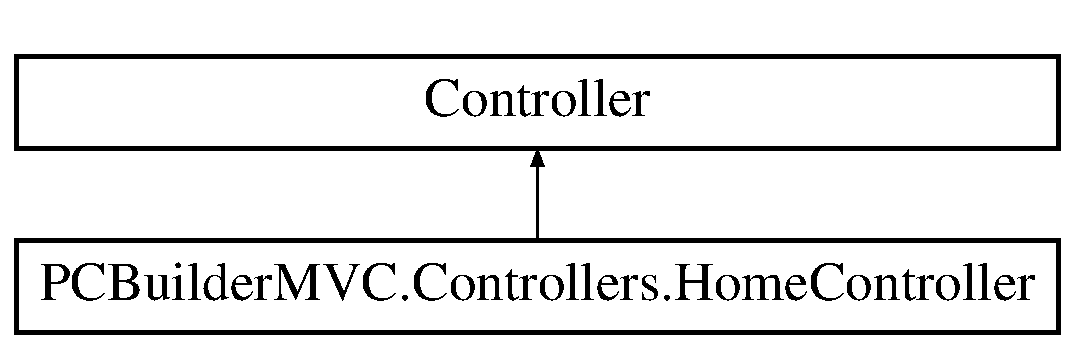
\includegraphics[height=2.000000cm]{class_p_c_builder_m_v_c_1_1_controllers_1_1_home_controller}
\end{center}
\end{figure}
\subsection*{Public Member Functions}
\begin{DoxyCompactItemize}
\item 
Action\+Result {\bfseries Index} ()\hypertarget{class_p_c_builder_m_v_c_1_1_controllers_1_1_home_controller_a801d32817dc4293c2f8e33c691ada19f}{}\label{class_p_c_builder_m_v_c_1_1_controllers_1_1_home_controller_a801d32817dc4293c2f8e33c691ada19f}

\item 
Action\+Result {\bfseries About} ()\hypertarget{class_p_c_builder_m_v_c_1_1_controllers_1_1_home_controller_a8890fc72d17ba59929e1dea4020a93a8}{}\label{class_p_c_builder_m_v_c_1_1_controllers_1_1_home_controller_a8890fc72d17ba59929e1dea4020a93a8}

\item 
Action\+Result {\bfseries Contact} ()\hypertarget{class_p_c_builder_m_v_c_1_1_controllers_1_1_home_controller_aede11cb947edcbe91f408801ad549d89}{}\label{class_p_c_builder_m_v_c_1_1_controllers_1_1_home_controller_aede11cb947edcbe91f408801ad549d89}

\end{DoxyCompactItemize}


\subsection{Detailed Description}
Home controller class to handle Home views interaction. 

\begin{DoxySeeAlso}{See also}
System.\+Web.\+Mvc.\+Controller


\end{DoxySeeAlso}


Definition at line 13 of file Home\+Controller.\+cs.



The documentation for this class was generated from the following file\+:\begin{DoxyCompactItemize}
\item 
C\+:/\+Users/nh228u08/\+Desktop/\+Final\+Project/\+Final\+Project/\+P\+C\+Builder/\+P\+C\+Builder\+M\+V\+C/\+Controllers/Home\+Controller.\+cs\end{DoxyCompactItemize}

\hypertarget{interface_business_logic_1_1_i_build_processor}{}\section{Business\+Logic.\+I\+Build\+Processor Interface Reference}
\label{interface_business_logic_1_1_i_build_processor}\index{Business\+Logic.\+I\+Build\+Processor@{Business\+Logic.\+I\+Build\+Processor}}
Inheritance diagram for Business\+Logic.\+I\+Build\+Processor\+:\begin{figure}[H]
\begin{center}
\leavevmode
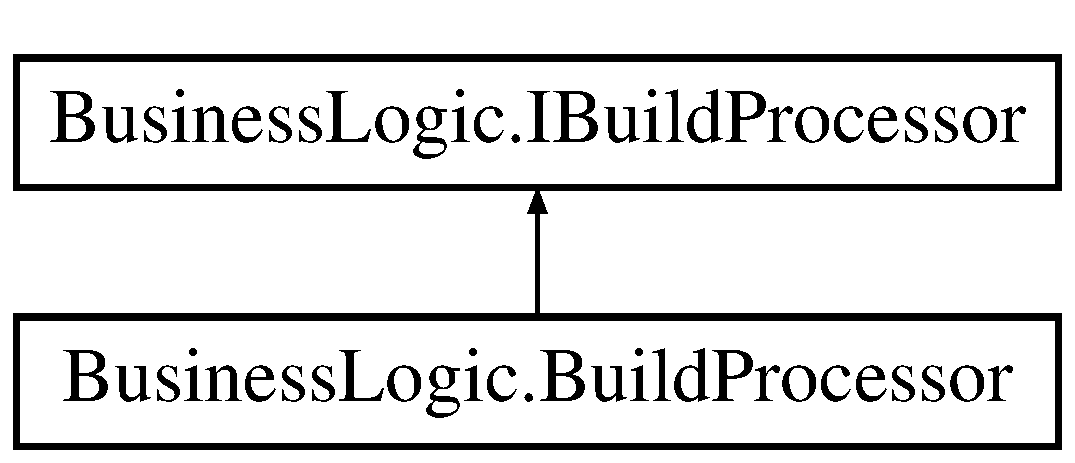
\includegraphics[height=2.000000cm]{interface_business_logic_1_1_i_build_processor}
\end{center}
\end{figure}
\subsection*{Public Member Functions}
\begin{DoxyCompactItemize}
\item 
\hyperlink{class_business_objects_1_1_finalized_build}{Finalized\+Build} {\bfseries Data\+Builder} (\hyperlink{class_business_objects_1_1_questionnaire_results}{Questionnaire\+Results} qr)\hypertarget{interface_business_logic_1_1_i_build_processor_a2e4fceb9979edca1ba6a37a45eb21608}{}\label{interface_business_logic_1_1_i_build_processor_a2e4fceb9979edca1ba6a37a45eb21608}

\end{DoxyCompactItemize}


\subsection{Detailed Description}


Definition at line 5 of file I\+Build\+Processor.\+cs.



The documentation for this interface was generated from the following file\+:\begin{DoxyCompactItemize}
\item 
C\+:/\+Users/nh228u08/\+Desktop/\+Final\+Project/\+Final\+Project/\+P\+C\+Builder/\+Business\+Logic/I\+Build\+Processor.\+cs\end{DoxyCompactItemize}

\hypertarget{class_p_c_builder_m_v_c_1_1_migrations_1_1_initial_create}{}\section{P\+C\+Builder\+M\+V\+C.\+Migrations.\+Initial\+Create Class Reference}
\label{class_p_c_builder_m_v_c_1_1_migrations_1_1_initial_create}\index{P\+C\+Builder\+M\+V\+C.\+Migrations.\+Initial\+Create@{P\+C\+Builder\+M\+V\+C.\+Migrations.\+Initial\+Create}}
Inheritance diagram for P\+C\+Builder\+M\+V\+C.\+Migrations.\+Initial\+Create\+:\begin{figure}[H]
\begin{center}
\leavevmode
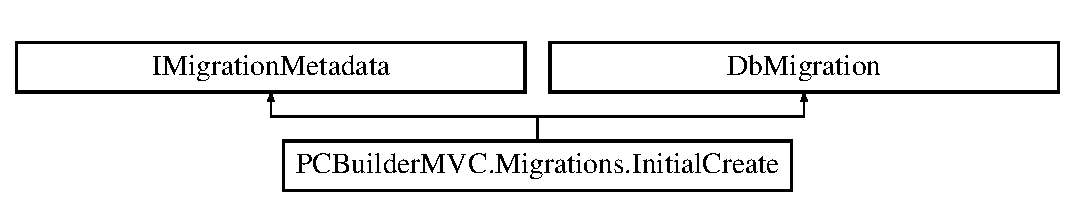
\includegraphics[height=2.000000cm]{class_p_c_builder_m_v_c_1_1_migrations_1_1_initial_create}
\end{center}
\end{figure}
\subsection*{Public Member Functions}
\begin{DoxyCompactItemize}
\item 
override void {\bfseries Up} ()\hypertarget{class_p_c_builder_m_v_c_1_1_migrations_1_1_initial_create_ae19a5b764e8e812350c7ed3235ddd828}{}\label{class_p_c_builder_m_v_c_1_1_migrations_1_1_initial_create_ae19a5b764e8e812350c7ed3235ddd828}

\item 
override void {\bfseries Down} ()\hypertarget{class_p_c_builder_m_v_c_1_1_migrations_1_1_initial_create_aa37b4ae0ed69ba9868659227304c67c1}{}\label{class_p_c_builder_m_v_c_1_1_migrations_1_1_initial_create_aa37b4ae0ed69ba9868659227304c67c1}

\end{DoxyCompactItemize}
\subsection*{Properties}
\begin{DoxyCompactItemize}
\item 
string I\+Migration\+Metadata. {\bfseries Id}\hspace{0.3cm}{\ttfamily  \mbox{[}get\mbox{]}}\hypertarget{class_p_c_builder_m_v_c_1_1_migrations_1_1_initial_create_a6f9793a927dbeb219230374d3005eba3}{}\label{class_p_c_builder_m_v_c_1_1_migrations_1_1_initial_create_a6f9793a927dbeb219230374d3005eba3}

\item 
string I\+Migration\+Metadata. {\bfseries Source}\hspace{0.3cm}{\ttfamily  \mbox{[}get\mbox{]}}\hypertarget{class_p_c_builder_m_v_c_1_1_migrations_1_1_initial_create_a3b3d2461ddd6849256eef839035d38f8}{}\label{class_p_c_builder_m_v_c_1_1_migrations_1_1_initial_create_a3b3d2461ddd6849256eef839035d38f8}

\item 
string I\+Migration\+Metadata. {\bfseries Target}\hspace{0.3cm}{\ttfamily  \mbox{[}get\mbox{]}}\hypertarget{class_p_c_builder_m_v_c_1_1_migrations_1_1_initial_create_aed09fd7f64406fc05ecebf1f10291f18}{}\label{class_p_c_builder_m_v_c_1_1_migrations_1_1_initial_create_aed09fd7f64406fc05ecebf1f10291f18}

\end{DoxyCompactItemize}
\subsection*{Private Attributes}
\begin{DoxyCompactItemize}
\item 
readonly Resource\+Manager {\bfseries Resources} = new Resource\+Manager(typeof(\hyperlink{class_p_c_builder_m_v_c_1_1_migrations_1_1_initial_create}{Initial\+Create}))\hypertarget{class_p_c_builder_m_v_c_1_1_migrations_1_1_initial_create_ac240ed5b2227a317b3b714c34ab01538}{}\label{class_p_c_builder_m_v_c_1_1_migrations_1_1_initial_create_ac240ed5b2227a317b3b714c34ab01538}

\end{DoxyCompactItemize}


\subsection{Detailed Description}


Definition at line 6 of file 201605040324555\+\_\+\+Initial\+Create.\+cs.



The documentation for this class was generated from the following files\+:\begin{DoxyCompactItemize}
\item 
C\+:/\+Users/nh228u08/\+Desktop/\+Final\+Project/\+Final\+Project/\+P\+C\+Builder/\+P\+C\+Builder\+M\+V\+C/\+Migrations/201605040324555\+\_\+\+Initial\+Create.\+cs\item 
C\+:/\+Users/nh228u08/\+Desktop/\+Final\+Project/\+Final\+Project/\+P\+C\+Builder/\+P\+C\+Builder\+M\+V\+C/\+Migrations/201605040324555\+\_\+\+Initial\+Create.\+Designer.\+cs\end{DoxyCompactItemize}

\hypertarget{class_p_c_builder_forms_1_1_log_in}{}\section{P\+C\+Builder\+Forms.\+Log\+In Class Reference}
\label{class_p_c_builder_forms_1_1_log_in}\index{P\+C\+Builder\+Forms.\+Log\+In@{P\+C\+Builder\+Forms.\+Log\+In}}


Interaction logic for Log\+In.\+xaml  


Inheritance diagram for P\+C\+Builder\+Forms.\+Log\+In\+:\begin{figure}[H]
\begin{center}
\leavevmode
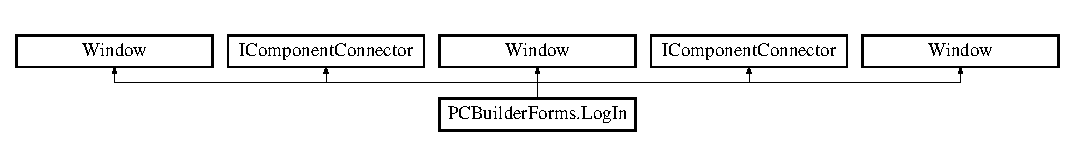
\includegraphics[height=1.523810cm]{class_p_c_builder_forms_1_1_log_in}
\end{center}
\end{figure}
\subsection*{Public Member Functions}
\begin{DoxyCompactItemize}
\item 
\hyperlink{class_p_c_builder_forms_1_1_log_in_a6a3ae2b82b608bdcdd99070a94e3a7c0}{Log\+In} ()
\begin{DoxyCompactList}\small\item\em Initializes a new instance of the \hyperlink{class_p_c_builder_forms_1_1_log_in}{Log\+In} class. \end{DoxyCompactList}\item 
void \hyperlink{class_p_c_builder_forms_1_1_log_in_ae0b7f84ba6cfe669a10e079fda5ab05d}{Initialize\+Component} ()
\begin{DoxyCompactList}\small\item\em Initialize\+Component \end{DoxyCompactList}\item 
void \hyperlink{class_p_c_builder_forms_1_1_log_in_ae0b7f84ba6cfe669a10e079fda5ab05d}{Initialize\+Component} ()
\begin{DoxyCompactList}\small\item\em Initialize\+Component \end{DoxyCompactList}\end{DoxyCompactItemize}
\subsection*{Public Attributes}
\begin{DoxyCompactItemize}
\item 
\hyperlink{class_business_objects_1_1_access_token}{Access\+Token} {\bfseries \+\_\+access\+Token}\hypertarget{class_p_c_builder_forms_1_1_log_in_a14d70ed974c56e1a0b92cc3c7b9f23da}{}\label{class_p_c_builder_forms_1_1_log_in_a14d70ed974c56e1a0b92cc3c7b9f23da}

\end{DoxyCompactItemize}
\subsection*{Package Attributes}
\begin{DoxyCompactItemize}
\item 
System.\+Windows.\+Controls.\+Label {\bfseries lbl\+Username}\hypertarget{class_p_c_builder_forms_1_1_log_in_ab7bcba65c47e51c34858cce414f2decd}{}\label{class_p_c_builder_forms_1_1_log_in_ab7bcba65c47e51c34858cce414f2decd}

\item 
System.\+Windows.\+Controls.\+Label {\bfseries lbl\+Password}\hypertarget{class_p_c_builder_forms_1_1_log_in_af3bf711dc3b2e7afdcf0b47d5c097416}{}\label{class_p_c_builder_forms_1_1_log_in_af3bf711dc3b2e7afdcf0b47d5c097416}

\item 
System.\+Windows.\+Controls.\+Label {\bfseries lbl\+Pass\+Confirm}\hypertarget{class_p_c_builder_forms_1_1_log_in_a18403b2be197f23358cf073b10360a07}{}\label{class_p_c_builder_forms_1_1_log_in_a18403b2be197f23358cf073b10360a07}

\item 
System.\+Windows.\+Controls.\+Label {\bfseries lbl\+First\+Name}\hypertarget{class_p_c_builder_forms_1_1_log_in_a2cee60babe4afc16f12049c744f9158a}{}\label{class_p_c_builder_forms_1_1_log_in_a2cee60babe4afc16f12049c744f9158a}

\item 
System.\+Windows.\+Controls.\+Label {\bfseries lbl\+Last\+Name}\hypertarget{class_p_c_builder_forms_1_1_log_in_a387bedcbb2e3e91e52f1c7d439fdc4a5}{}\label{class_p_c_builder_forms_1_1_log_in_a387bedcbb2e3e91e52f1c7d439fdc4a5}

\item 
System.\+Windows.\+Controls.\+Label {\bfseries lbl\+Address}\hypertarget{class_p_c_builder_forms_1_1_log_in_a38bc4cccf50c7d73b71e1061a8b6f918}{}\label{class_p_c_builder_forms_1_1_log_in_a38bc4cccf50c7d73b71e1061a8b6f918}

\item 
System.\+Windows.\+Controls.\+Label {\bfseries lbl\+City}\hypertarget{class_p_c_builder_forms_1_1_log_in_a892e206664f293f6fd7e58487b7e0ab7}{}\label{class_p_c_builder_forms_1_1_log_in_a892e206664f293f6fd7e58487b7e0ab7}

\item 
System.\+Windows.\+Controls.\+Label {\bfseries lbl\+State}\hypertarget{class_p_c_builder_forms_1_1_log_in_a7602a0f2fbd4d339609b3ed43bf1cab0}{}\label{class_p_c_builder_forms_1_1_log_in_a7602a0f2fbd4d339609b3ed43bf1cab0}

\item 
System.\+Windows.\+Controls.\+Label {\bfseries lbl\+Zip}\hypertarget{class_p_c_builder_forms_1_1_log_in_a95335e4f306d140c479af8d212d1c59a}{}\label{class_p_c_builder_forms_1_1_log_in_a95335e4f306d140c479af8d212d1c59a}

\item 
System.\+Windows.\+Controls.\+Label {\bfseries lbl\+Phone}\hypertarget{class_p_c_builder_forms_1_1_log_in_a8bfcacc207daa48f971cf88164c74f56}{}\label{class_p_c_builder_forms_1_1_log_in_a8bfcacc207daa48f971cf88164c74f56}

\item 
System.\+Windows.\+Controls.\+Label {\bfseries lbl\+Email}\hypertarget{class_p_c_builder_forms_1_1_log_in_a9f5d1f353476f6b81dd5c23226d3fb6a}{}\label{class_p_c_builder_forms_1_1_log_in_a9f5d1f353476f6b81dd5c23226d3fb6a}

\item 
System.\+Windows.\+Controls.\+Text\+Box {\bfseries txt\+Username}\hypertarget{class_p_c_builder_forms_1_1_log_in_aa9446489f0e9e0896303b3430fade22d}{}\label{class_p_c_builder_forms_1_1_log_in_aa9446489f0e9e0896303b3430fade22d}

\item 
System.\+Windows.\+Controls.\+Password\+Box {\bfseries txt\+Password}\hypertarget{class_p_c_builder_forms_1_1_log_in_a0b81eaa25cb2868469292fa55b51d76c}{}\label{class_p_c_builder_forms_1_1_log_in_a0b81eaa25cb2868469292fa55b51d76c}

\item 
System.\+Windows.\+Controls.\+Password\+Box {\bfseries txt\+Pass\+Confirm}\hypertarget{class_p_c_builder_forms_1_1_log_in_ac6db00a879be9036ed5582977d99e54c}{}\label{class_p_c_builder_forms_1_1_log_in_ac6db00a879be9036ed5582977d99e54c}

\item 
System.\+Windows.\+Controls.\+Text\+Box {\bfseries txt\+First\+Name}\hypertarget{class_p_c_builder_forms_1_1_log_in_a0a3383d92461671843f1e81bf3c1ba7f}{}\label{class_p_c_builder_forms_1_1_log_in_a0a3383d92461671843f1e81bf3c1ba7f}

\item 
System.\+Windows.\+Controls.\+Text\+Box {\bfseries txt\+Last\+Name}\hypertarget{class_p_c_builder_forms_1_1_log_in_aff9a595a21cb6de8311772d714ee3baf}{}\label{class_p_c_builder_forms_1_1_log_in_aff9a595a21cb6de8311772d714ee3baf}

\item 
System.\+Windows.\+Controls.\+Text\+Box {\bfseries txt\+Address}\hypertarget{class_p_c_builder_forms_1_1_log_in_a058d08c9916e931de9e971766c46aa5a}{}\label{class_p_c_builder_forms_1_1_log_in_a058d08c9916e931de9e971766c46aa5a}

\item 
System.\+Windows.\+Controls.\+Text\+Box {\bfseries txt\+City}\hypertarget{class_p_c_builder_forms_1_1_log_in_ad58fc7528dd38b267cf69ad727f4f540}{}\label{class_p_c_builder_forms_1_1_log_in_ad58fc7528dd38b267cf69ad727f4f540}

\item 
System.\+Windows.\+Controls.\+Text\+Box {\bfseries txt\+State}\hypertarget{class_p_c_builder_forms_1_1_log_in_acb6869b9d62d240935fdf7a30d374312}{}\label{class_p_c_builder_forms_1_1_log_in_acb6869b9d62d240935fdf7a30d374312}

\item 
System.\+Windows.\+Controls.\+Text\+Box {\bfseries txt\+Zip}\hypertarget{class_p_c_builder_forms_1_1_log_in_afea046faf47b1315035c8f7ff5d4e33e}{}\label{class_p_c_builder_forms_1_1_log_in_afea046faf47b1315035c8f7ff5d4e33e}

\item 
System.\+Windows.\+Controls.\+Text\+Box {\bfseries txt\+Phone}\hypertarget{class_p_c_builder_forms_1_1_log_in_a154f33f4ae0b8c376a28c7af29743a73}{}\label{class_p_c_builder_forms_1_1_log_in_a154f33f4ae0b8c376a28c7af29743a73}

\item 
System.\+Windows.\+Controls.\+Text\+Box {\bfseries txt\+Email}\hypertarget{class_p_c_builder_forms_1_1_log_in_a49b9b1917d282c3bdd50c09225fcff96}{}\label{class_p_c_builder_forms_1_1_log_in_a49b9b1917d282c3bdd50c09225fcff96}

\item 
System.\+Windows.\+Controls.\+Check\+Box {\bfseries chk\+New\+User}\hypertarget{class_p_c_builder_forms_1_1_log_in_ab87fa6f5a4a6a03863fcdc55415ca463}{}\label{class_p_c_builder_forms_1_1_log_in_ab87fa6f5a4a6a03863fcdc55415ca463}

\item 
System.\+Windows.\+Controls.\+Button {\bfseries btn\+Submit}\hypertarget{class_p_c_builder_forms_1_1_log_in_ae16bbcdb8825c3c20581dcd102081053}{}\label{class_p_c_builder_forms_1_1_log_in_ae16bbcdb8825c3c20581dcd102081053}

\item 
System.\+Windows.\+Controls.\+Button {\bfseries btn\+Cancel}\hypertarget{class_p_c_builder_forms_1_1_log_in_a14ee67f6d0363e194c50086339cbd8c5}{}\label{class_p_c_builder_forms_1_1_log_in_a14ee67f6d0363e194c50086339cbd8c5}

\end{DoxyCompactItemize}
\subsection*{Private Member Functions}
\begin{DoxyCompactItemize}
\item 
void \hyperlink{class_p_c_builder_forms_1_1_log_in_a42186d8ab10ba7fefbe6d93fe0686046}{chk\+New\+User\+\_\+\+Checked} (object sender, Routed\+Event\+Args e)
\begin{DoxyCompactList}\small\item\em Handles the Checked event of the chk\+New\+User control. \end{DoxyCompactList}\item 
void \hyperlink{class_p_c_builder_forms_1_1_log_in_a82887e13a948dfad13c8f33758ae2e27}{chk\+New\+User\+\_\+\+Unchecked} (object sender, Routed\+Event\+Args e)
\begin{DoxyCompactList}\small\item\em Handles the Unchecked event of the chk\+New\+User control. \end{DoxyCompactList}\item 
void \hyperlink{class_p_c_builder_forms_1_1_log_in_a5bd038fb92b73172d645fb1c0b754a25}{btn\+Submit\+\_\+\+Click} (object sender, Routed\+Event\+Args e)
\begin{DoxyCompactList}\small\item\em Handles the Click event of the btn\+Submit control. \end{DoxyCompactList}\item 
void \hyperlink{class_p_c_builder_forms_1_1_log_in_af358b3dce8bd658650e92a6974c923bb}{btn\+Cancel\+\_\+\+Click} (object sender, Routed\+Event\+Args e)
\begin{DoxyCompactList}\small\item\em Handles the Click event of the btn\+Cancel control. \end{DoxyCompactList}\item 
void System.\+Windows.\+Markup.\+I\+Component\+Connector. {\bfseries Connect} (int connection\+Id, object target)\hypertarget{class_p_c_builder_forms_1_1_log_in_ac680078b371585945fb49de677d48bfd}{}\label{class_p_c_builder_forms_1_1_log_in_ac680078b371585945fb49de677d48bfd}

\item 
void System.\+Windows.\+Markup.\+I\+Component\+Connector. {\bfseries Connect} (int connection\+Id, object target)\hypertarget{class_p_c_builder_forms_1_1_log_in_ac680078b371585945fb49de677d48bfd}{}\label{class_p_c_builder_forms_1_1_log_in_ac680078b371585945fb49de677d48bfd}

\end{DoxyCompactItemize}
\subsection*{Private Attributes}
\begin{DoxyCompactItemize}
\item 
bool {\bfseries \+\_\+content\+Loaded}\hypertarget{class_p_c_builder_forms_1_1_log_in_a41ad8d18307518e6429387ec9ad2189a}{}\label{class_p_c_builder_forms_1_1_log_in_a41ad8d18307518e6429387ec9ad2189a}

\end{DoxyCompactItemize}


\subsection{Detailed Description}
Interaction logic for Log\+In.\+xaml 

\hyperlink{class_p_c_builder_forms_1_1_log_in}{Log\+In} 

Definition at line 21 of file Log\+In.\+xaml.\+cs.



\subsection{Constructor \& Destructor Documentation}
\index{P\+C\+Builder\+Forms\+::\+Log\+In@{P\+C\+Builder\+Forms\+::\+Log\+In}!Log\+In@{Log\+In}}
\index{Log\+In@{Log\+In}!P\+C\+Builder\+Forms\+::\+Log\+In@{P\+C\+Builder\+Forms\+::\+Log\+In}}
\subsubsection[{\texorpdfstring{Log\+In()}{LogIn()}}]{\setlength{\rightskip}{0pt plus 5cm}P\+C\+Builder\+Forms.\+Log\+In.\+Log\+In (
\begin{DoxyParamCaption}
{}
\end{DoxyParamCaption}
)}\hypertarget{class_p_c_builder_forms_1_1_log_in_a6a3ae2b82b608bdcdd99070a94e3a7c0}{}\label{class_p_c_builder_forms_1_1_log_in_a6a3ae2b82b608bdcdd99070a94e3a7c0}


Initializes a new instance of the \hyperlink{class_p_c_builder_forms_1_1_log_in}{Log\+In} class. 



Definition at line 28 of file Log\+In.\+xaml.\+cs.



\subsection{Member Function Documentation}
\index{P\+C\+Builder\+Forms\+::\+Log\+In@{P\+C\+Builder\+Forms\+::\+Log\+In}!btn\+Cancel\+\_\+\+Click@{btn\+Cancel\+\_\+\+Click}}
\index{btn\+Cancel\+\_\+\+Click@{btn\+Cancel\+\_\+\+Click}!P\+C\+Builder\+Forms\+::\+Log\+In@{P\+C\+Builder\+Forms\+::\+Log\+In}}
\subsubsection[{\texorpdfstring{btn\+Cancel\+\_\+\+Click(object sender, Routed\+Event\+Args e)}{btnCancel_Click(object sender, RoutedEventArgs e)}}]{\setlength{\rightskip}{0pt plus 5cm}void P\+C\+Builder\+Forms.\+Log\+In.\+btn\+Cancel\+\_\+\+Click (
\begin{DoxyParamCaption}
\item[{object}]{sender, }
\item[{Routed\+Event\+Args}]{e}
\end{DoxyParamCaption}
)\hspace{0.3cm}{\ttfamily [private]}}\hypertarget{class_p_c_builder_forms_1_1_log_in_af358b3dce8bd658650e92a6974c923bb}{}\label{class_p_c_builder_forms_1_1_log_in_af358b3dce8bd658650e92a6974c923bb}


Handles the Click event of the btn\+Cancel control. 


\begin{DoxyParams}{Parameters}
{\em sender} & The source of the event.\\
\hline
{\em e} & The Routed\+Event\+Args instance containing the event data.\\
\hline
\end{DoxyParams}


Definition at line 141 of file Log\+In.\+xaml.\+cs.

\index{P\+C\+Builder\+Forms\+::\+Log\+In@{P\+C\+Builder\+Forms\+::\+Log\+In}!btn\+Submit\+\_\+\+Click@{btn\+Submit\+\_\+\+Click}}
\index{btn\+Submit\+\_\+\+Click@{btn\+Submit\+\_\+\+Click}!P\+C\+Builder\+Forms\+::\+Log\+In@{P\+C\+Builder\+Forms\+::\+Log\+In}}
\subsubsection[{\texorpdfstring{btn\+Submit\+\_\+\+Click(object sender, Routed\+Event\+Args e)}{btnSubmit_Click(object sender, RoutedEventArgs e)}}]{\setlength{\rightskip}{0pt plus 5cm}void P\+C\+Builder\+Forms.\+Log\+In.\+btn\+Submit\+\_\+\+Click (
\begin{DoxyParamCaption}
\item[{object}]{sender, }
\item[{Routed\+Event\+Args}]{e}
\end{DoxyParamCaption}
)\hspace{0.3cm}{\ttfamily [private]}}\hypertarget{class_p_c_builder_forms_1_1_log_in_a5bd038fb92b73172d645fb1c0b754a25}{}\label{class_p_c_builder_forms_1_1_log_in_a5bd038fb92b73172d645fb1c0b754a25}


Handles the Click event of the btn\+Submit control. 


\begin{DoxyParams}{Parameters}
{\em sender} & The source of the event.\\
\hline
{\em e} & The Routed\+Event\+Args instance containing the event data.\\
\hline
\end{DoxyParams}


Definition at line 96 of file Log\+In.\+xaml.\+cs.

\index{P\+C\+Builder\+Forms\+::\+Log\+In@{P\+C\+Builder\+Forms\+::\+Log\+In}!chk\+New\+User\+\_\+\+Checked@{chk\+New\+User\+\_\+\+Checked}}
\index{chk\+New\+User\+\_\+\+Checked@{chk\+New\+User\+\_\+\+Checked}!P\+C\+Builder\+Forms\+::\+Log\+In@{P\+C\+Builder\+Forms\+::\+Log\+In}}
\subsubsection[{\texorpdfstring{chk\+New\+User\+\_\+\+Checked(object sender, Routed\+Event\+Args e)}{chkNewUser_Checked(object sender, RoutedEventArgs e)}}]{\setlength{\rightskip}{0pt plus 5cm}void P\+C\+Builder\+Forms.\+Log\+In.\+chk\+New\+User\+\_\+\+Checked (
\begin{DoxyParamCaption}
\item[{object}]{sender, }
\item[{Routed\+Event\+Args}]{e}
\end{DoxyParamCaption}
)\hspace{0.3cm}{\ttfamily [private]}}\hypertarget{class_p_c_builder_forms_1_1_log_in_a42186d8ab10ba7fefbe6d93fe0686046}{}\label{class_p_c_builder_forms_1_1_log_in_a42186d8ab10ba7fefbe6d93fe0686046}


Handles the Checked event of the chk\+New\+User control. 


\begin{DoxyParams}{Parameters}
{\em sender} & The source of the event.\\
\hline
{\em e} & The Routed\+Event\+Args instance containing the event data.\\
\hline
\end{DoxyParams}


Definition at line 38 of file Log\+In.\+xaml.\+cs.

\index{P\+C\+Builder\+Forms\+::\+Log\+In@{P\+C\+Builder\+Forms\+::\+Log\+In}!chk\+New\+User\+\_\+\+Unchecked@{chk\+New\+User\+\_\+\+Unchecked}}
\index{chk\+New\+User\+\_\+\+Unchecked@{chk\+New\+User\+\_\+\+Unchecked}!P\+C\+Builder\+Forms\+::\+Log\+In@{P\+C\+Builder\+Forms\+::\+Log\+In}}
\subsubsection[{\texorpdfstring{chk\+New\+User\+\_\+\+Unchecked(object sender, Routed\+Event\+Args e)}{chkNewUser_Unchecked(object sender, RoutedEventArgs e)}}]{\setlength{\rightskip}{0pt plus 5cm}void P\+C\+Builder\+Forms.\+Log\+In.\+chk\+New\+User\+\_\+\+Unchecked (
\begin{DoxyParamCaption}
\item[{object}]{sender, }
\item[{Routed\+Event\+Args}]{e}
\end{DoxyParamCaption}
)\hspace{0.3cm}{\ttfamily [private]}}\hypertarget{class_p_c_builder_forms_1_1_log_in_a82887e13a948dfad13c8f33758ae2e27}{}\label{class_p_c_builder_forms_1_1_log_in_a82887e13a948dfad13c8f33758ae2e27}


Handles the Unchecked event of the chk\+New\+User control. 


\begin{DoxyParams}{Parameters}
{\em sender} & The source of the event.\\
\hline
{\em e} & The Routed\+Event\+Args instance containing the event data.\\
\hline
\end{DoxyParams}


Definition at line 67 of file Log\+In.\+xaml.\+cs.

\index{P\+C\+Builder\+Forms\+::\+Log\+In@{P\+C\+Builder\+Forms\+::\+Log\+In}!Initialize\+Component@{Initialize\+Component}}
\index{Initialize\+Component@{Initialize\+Component}!P\+C\+Builder\+Forms\+::\+Log\+In@{P\+C\+Builder\+Forms\+::\+Log\+In}}
\subsubsection[{\texorpdfstring{Initialize\+Component()}{InitializeComponent()}}]{\setlength{\rightskip}{0pt plus 5cm}void P\+C\+Builder\+Forms.\+Log\+In.\+Initialize\+Component (
\begin{DoxyParamCaption}
{}
\end{DoxyParamCaption}
)}\hypertarget{class_p_c_builder_forms_1_1_log_in_ae0b7f84ba6cfe669a10e079fda5ab05d}{}\label{class_p_c_builder_forms_1_1_log_in_ae0b7f84ba6cfe669a10e079fda5ab05d}


Initialize\+Component 



Definition at line 250 of file Log\+In.\+g.\+i.\+cs.

\index{P\+C\+Builder\+Forms\+::\+Log\+In@{P\+C\+Builder\+Forms\+::\+Log\+In}!Initialize\+Component@{Initialize\+Component}}
\index{Initialize\+Component@{Initialize\+Component}!P\+C\+Builder\+Forms\+::\+Log\+In@{P\+C\+Builder\+Forms\+::\+Log\+In}}
\subsubsection[{\texorpdfstring{Initialize\+Component()}{InitializeComponent()}}]{\setlength{\rightskip}{0pt plus 5cm}void P\+C\+Builder\+Forms.\+Log\+In.\+Initialize\+Component (
\begin{DoxyParamCaption}
{}
\end{DoxyParamCaption}
)}\hypertarget{class_p_c_builder_forms_1_1_log_in_ae0b7f84ba6cfe669a10e079fda5ab05d}{}\label{class_p_c_builder_forms_1_1_log_in_ae0b7f84ba6cfe669a10e079fda5ab05d}


Initialize\+Component 



Definition at line 250 of file Log\+In.\+g.\+cs.



The documentation for this class was generated from the following files\+:\begin{DoxyCompactItemize}
\item 
C\+:/\+Users/nh228u08/\+Desktop/\+Final\+Project/\+Final\+Project/\+P\+C\+Builder/\+P\+C\+Builder\+Forms/Log\+In.\+xaml.\+cs\item 
C\+:/\+Users/nh228u08/\+Desktop/\+Final\+Project/\+Final\+Project/\+P\+C\+Builder/\+P\+C\+Builder\+Forms/obj/\+Debug/Log\+In.\+g.\+cs\item 
C\+:/\+Users/nh228u08/\+Desktop/\+Final\+Project/\+Final\+Project/\+P\+C\+Builder/\+P\+C\+Builder\+Forms/obj/\+Debug/Log\+In.\+g.\+i.\+cs\end{DoxyCompactItemize}

\hypertarget{class_p_c_builder_m_v_c_1_1_models_1_1_login_view_model}{}\section{P\+C\+Builder\+M\+V\+C.\+Models.\+Login\+View\+Model Class Reference}
\label{class_p_c_builder_m_v_c_1_1_models_1_1_login_view_model}\index{P\+C\+Builder\+M\+V\+C.\+Models.\+Login\+View\+Model@{P\+C\+Builder\+M\+V\+C.\+Models.\+Login\+View\+Model}}


Login view model class.  


\subsection*{Properties}
\begin{DoxyCompactItemize}
\item 
string {\bfseries Email}\hspace{0.3cm}{\ttfamily  \mbox{[}get, set\mbox{]}}\hypertarget{class_p_c_builder_m_v_c_1_1_models_1_1_login_view_model_aad5041cce607cd8effdcd1f74ad01c76}{}\label{class_p_c_builder_m_v_c_1_1_models_1_1_login_view_model_aad5041cce607cd8effdcd1f74ad01c76}

\item 
string {\bfseries Password}\hspace{0.3cm}{\ttfamily  \mbox{[}get, set\mbox{]}}\hypertarget{class_p_c_builder_m_v_c_1_1_models_1_1_login_view_model_af897b8fd8d37fb9c3c96fbdda9e2b7fa}{}\label{class_p_c_builder_m_v_c_1_1_models_1_1_login_view_model_af897b8fd8d37fb9c3c96fbdda9e2b7fa}

\item 
bool {\bfseries Remember\+Me}\hspace{0.3cm}{\ttfamily  \mbox{[}get, set\mbox{]}}\hypertarget{class_p_c_builder_m_v_c_1_1_models_1_1_login_view_model_a10f675dd23224511e3c9a1b9c7d1c3e4}{}\label{class_p_c_builder_m_v_c_1_1_models_1_1_login_view_model_a10f675dd23224511e3c9a1b9c7d1c3e4}

\end{DoxyCompactItemize}


\subsection{Detailed Description}
Login view model class. 



Definition at line 50 of file Account\+View\+Models.\+cs.



The documentation for this class was generated from the following file\+:\begin{DoxyCompactItemize}
\item 
C\+:/\+Users/nh228u08/\+Desktop/\+Final\+Project/\+Final\+Project/\+P\+C\+Builder/\+P\+C\+Builder\+M\+V\+C/\+Models/Account\+View\+Models.\+cs\end{DoxyCompactItemize}

\hypertarget{class_p_c_builder_forms_1_1_main_window}{}\section{P\+C\+Builder\+Forms.\+Main\+Window Class Reference}
\label{class_p_c_builder_forms_1_1_main_window}\index{P\+C\+Builder\+Forms.\+Main\+Window@{P\+C\+Builder\+Forms.\+Main\+Window}}


Interaction logic for Main\+Window.\+xaml  


Inheritance diagram for P\+C\+Builder\+Forms.\+Main\+Window\+:\begin{figure}[H]
\begin{center}
\leavevmode
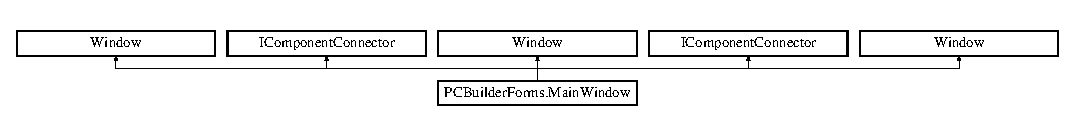
\includegraphics[height=1.191489cm]{class_p_c_builder_forms_1_1_main_window}
\end{center}
\end{figure}
\subsection*{Public Member Functions}
\begin{DoxyCompactItemize}
\item 
\hyperlink{class_p_c_builder_forms_1_1_main_window_a6201f6763f4ee3b2188d9ec18a9fa881}{Main\+Window} ()
\begin{DoxyCompactList}\small\item\em Initializes a new instance of the \hyperlink{class_p_c_builder_forms_1_1_main_window}{Main\+Window} class. \end{DoxyCompactList}\item 
void \hyperlink{class_p_c_builder_forms_1_1_main_window_af61d622148f662bb5060f1523fae41ae}{Initialize\+Component} ()
\begin{DoxyCompactList}\small\item\em Initialize\+Component \end{DoxyCompactList}\item 
void \hyperlink{class_p_c_builder_forms_1_1_main_window_af61d622148f662bb5060f1523fae41ae}{Initialize\+Component} ()
\begin{DoxyCompactList}\small\item\em Initialize\+Component \end{DoxyCompactList}\end{DoxyCompactItemize}
\subsection*{Package Attributes}
\begin{DoxyCompactItemize}
\item 
System.\+Windows.\+Controls.\+Menu\+Item {\bfseries mnu\+Exit}\hypertarget{class_p_c_builder_forms_1_1_main_window_a53d466d670b9f69781a4139799ebe80b}{}\label{class_p_c_builder_forms_1_1_main_window_a53d466d670b9f69781a4139799ebe80b}

\item 
System.\+Windows.\+Controls.\+Label {\bfseries lbl\+Login\+Message}\hypertarget{class_p_c_builder_forms_1_1_main_window_a3d07af2e8da4efc0b3cc6d267e2bbd4d}{}\label{class_p_c_builder_forms_1_1_main_window_a3d07af2e8da4efc0b3cc6d267e2bbd4d}

\item 
System.\+Windows.\+Controls.\+Button {\bfseries btn\+Login}\hypertarget{class_p_c_builder_forms_1_1_main_window_ade2269fd046864f55446ebc6df1861cf}{}\label{class_p_c_builder_forms_1_1_main_window_ade2269fd046864f55446ebc6df1861cf}

\item 
System.\+Windows.\+Controls.\+Tab\+Item {\bfseries tab\+Build\+A\+PC}\hypertarget{class_p_c_builder_forms_1_1_main_window_ae351e6ef4dd06c9130510b0dfb0e42c6}{}\label{class_p_c_builder_forms_1_1_main_window_ae351e6ef4dd06c9130510b0dfb0e42c6}

\item 
System.\+Windows.\+Controls.\+Button {\bfseries btn\+Questionnaire}\hypertarget{class_p_c_builder_forms_1_1_main_window_a686049c1273b758aa8cb90d6df28c66e}{}\label{class_p_c_builder_forms_1_1_main_window_a686049c1273b758aa8cb90d6df28c66e}

\item 
System.\+Windows.\+Controls.\+Tab\+Item {\bfseries tab\+Build\+Output}\hypertarget{class_p_c_builder_forms_1_1_main_window_a8a08f6b04a5758d518c6a477eb760dc0}{}\label{class_p_c_builder_forms_1_1_main_window_a8a08f6b04a5758d518c6a477eb760dc0}

\item 
System.\+Windows.\+Controls.\+Label {\bfseries lbl\+Cpu\+Brand}\hypertarget{class_p_c_builder_forms_1_1_main_window_a4beec0d4e8d2f9be5a7a0e45065b40ae}{}\label{class_p_c_builder_forms_1_1_main_window_a4beec0d4e8d2f9be5a7a0e45065b40ae}

\item 
System.\+Windows.\+Controls.\+Label {\bfseries lbl\+Gpu\+Brand}\hypertarget{class_p_c_builder_forms_1_1_main_window_a55bff109b418e181a8b414800a16a63f}{}\label{class_p_c_builder_forms_1_1_main_window_a55bff109b418e181a8b414800a16a63f}

\item 
System.\+Windows.\+Controls.\+Label {\bfseries lbl\+Motherboard\+Brand}\hypertarget{class_p_c_builder_forms_1_1_main_window_ae80040a3f73acf0777b3ec0443c3b89e}{}\label{class_p_c_builder_forms_1_1_main_window_ae80040a3f73acf0777b3ec0443c3b89e}

\item 
System.\+Windows.\+Controls.\+Label {\bfseries lbl\+Optical\+Brand}\hypertarget{class_p_c_builder_forms_1_1_main_window_aa9dec4fd7c39204b849c0e5c773d08f8}{}\label{class_p_c_builder_forms_1_1_main_window_aa9dec4fd7c39204b849c0e5c773d08f8}

\item 
System.\+Windows.\+Controls.\+Label {\bfseries lbl\+Psu\+Brand}\hypertarget{class_p_c_builder_forms_1_1_main_window_a750db1e2aa6edaf0ea3fbc6df6a5cc5b}{}\label{class_p_c_builder_forms_1_1_main_window_a750db1e2aa6edaf0ea3fbc6df6a5cc5b}

\item 
System.\+Windows.\+Controls.\+Label {\bfseries lbl\+Ram\+Brand}\hypertarget{class_p_c_builder_forms_1_1_main_window_a142c704730f49d4b965477d68907d485}{}\label{class_p_c_builder_forms_1_1_main_window_a142c704730f49d4b965477d68907d485}

\item 
System.\+Windows.\+Controls.\+Label {\bfseries lbl\+Storage\+Brand}\hypertarget{class_p_c_builder_forms_1_1_main_window_a3bf0b669539a609c7e7e61eec0358d30}{}\label{class_p_c_builder_forms_1_1_main_window_a3bf0b669539a609c7e7e61eec0358d30}

\item 
System.\+Windows.\+Controls.\+Label {\bfseries lbl\+Cpu\+Model}\hypertarget{class_p_c_builder_forms_1_1_main_window_a5cc408a021d32c64e43e5ae2385ebe08}{}\label{class_p_c_builder_forms_1_1_main_window_a5cc408a021d32c64e43e5ae2385ebe08}

\item 
System.\+Windows.\+Controls.\+Label {\bfseries lbl\+Gpu\+Model}\hypertarget{class_p_c_builder_forms_1_1_main_window_a8b508ce0f02f46eca4b8464b4afa4b2a}{}\label{class_p_c_builder_forms_1_1_main_window_a8b508ce0f02f46eca4b8464b4afa4b2a}

\item 
System.\+Windows.\+Controls.\+Label {\bfseries lbl\+Motherboard\+Model}\hypertarget{class_p_c_builder_forms_1_1_main_window_af400f268e48340e87f8479d7c0391af1}{}\label{class_p_c_builder_forms_1_1_main_window_af400f268e48340e87f8479d7c0391af1}

\item 
System.\+Windows.\+Controls.\+Label {\bfseries lbl\+Optical\+Model}\hypertarget{class_p_c_builder_forms_1_1_main_window_ae2edb6353608d2c52ecc0a6ddbdcb602}{}\label{class_p_c_builder_forms_1_1_main_window_ae2edb6353608d2c52ecc0a6ddbdcb602}

\item 
System.\+Windows.\+Controls.\+Label {\bfseries lbl\+Psu\+Model}\hypertarget{class_p_c_builder_forms_1_1_main_window_a6d2c596ed32bfb3879e1242f908e5fe1}{}\label{class_p_c_builder_forms_1_1_main_window_a6d2c596ed32bfb3879e1242f908e5fe1}

\item 
System.\+Windows.\+Controls.\+Label {\bfseries lbl\+Ram\+Model}\hypertarget{class_p_c_builder_forms_1_1_main_window_ab5d31bdb94c3986c0b03354e4e2a0487}{}\label{class_p_c_builder_forms_1_1_main_window_ab5d31bdb94c3986c0b03354e4e2a0487}

\item 
System.\+Windows.\+Controls.\+Label {\bfseries lbl\+Storage\+Model}\hypertarget{class_p_c_builder_forms_1_1_main_window_acd1d1808b4f868ecd50dd15e2021864c}{}\label{class_p_c_builder_forms_1_1_main_window_acd1d1808b4f868ecd50dd15e2021864c}

\item 
System.\+Windows.\+Controls.\+Label {\bfseries lbl\+C\+P\+U\+Price}\hypertarget{class_p_c_builder_forms_1_1_main_window_a08fa4f8f707453efb3d85a53fa04c0d0}{}\label{class_p_c_builder_forms_1_1_main_window_a08fa4f8f707453efb3d85a53fa04c0d0}

\item 
System.\+Windows.\+Controls.\+Label {\bfseries lbl\+G\+P\+U\+Price}\hypertarget{class_p_c_builder_forms_1_1_main_window_a6cf92c3735ba782adcd9edfe7f812394}{}\label{class_p_c_builder_forms_1_1_main_window_a6cf92c3735ba782adcd9edfe7f812394}

\item 
System.\+Windows.\+Controls.\+Label {\bfseries lbl\+Motherboard\+Price}\hypertarget{class_p_c_builder_forms_1_1_main_window_a7691904b7c6835bfdddd8501ccf3d379}{}\label{class_p_c_builder_forms_1_1_main_window_a7691904b7c6835bfdddd8501ccf3d379}

\item 
System.\+Windows.\+Controls.\+Label {\bfseries lbl\+Optical\+Price}\hypertarget{class_p_c_builder_forms_1_1_main_window_a38790226817ed7fb5ba17fe7cb5a471d}{}\label{class_p_c_builder_forms_1_1_main_window_a38790226817ed7fb5ba17fe7cb5a471d}

\item 
System.\+Windows.\+Controls.\+Label {\bfseries lbl\+P\+S\+U\+Price}\hypertarget{class_p_c_builder_forms_1_1_main_window_a16dd937cd87eff6be41f3400f906e21e}{}\label{class_p_c_builder_forms_1_1_main_window_a16dd937cd87eff6be41f3400f906e21e}

\item 
System.\+Windows.\+Controls.\+Label {\bfseries lbl\+R\+A\+M\+Price}\hypertarget{class_p_c_builder_forms_1_1_main_window_a56e9d3fe56e1012c0685c1590089bf6b}{}\label{class_p_c_builder_forms_1_1_main_window_a56e9d3fe56e1012c0685c1590089bf6b}

\item 
System.\+Windows.\+Controls.\+Label {\bfseries lbl\+Storage\+Price}\hypertarget{class_p_c_builder_forms_1_1_main_window_aac3ae4c4d412f7ed2579b50f5bf49593}{}\label{class_p_c_builder_forms_1_1_main_window_aac3ae4c4d412f7ed2579b50f5bf49593}

\item 
System.\+Windows.\+Controls.\+Label {\bfseries lbl\+Total\+Price}\hypertarget{class_p_c_builder_forms_1_1_main_window_ad49dd04f2e8a7df276a86a1b0ed6e5d2}{}\label{class_p_c_builder_forms_1_1_main_window_ad49dd04f2e8a7df276a86a1b0ed6e5d2}

\item 
System.\+Windows.\+Controls.\+Tab\+Item {\bfseries tab\+Admin}\hypertarget{class_p_c_builder_forms_1_1_main_window_ab6f01653dcc72005e5ba59f5158b361f}{}\label{class_p_c_builder_forms_1_1_main_window_ab6f01653dcc72005e5ba59f5158b361f}

\item 
System.\+Windows.\+Controls.\+Button {\bfseries btn\+Add\+User}\hypertarget{class_p_c_builder_forms_1_1_main_window_a18b997d107efafb1c6e0f12910bb8715}{}\label{class_p_c_builder_forms_1_1_main_window_a18b997d107efafb1c6e0f12910bb8715}

\item 
System.\+Windows.\+Controls.\+Button {\bfseries btn\+Delete\+User}\hypertarget{class_p_c_builder_forms_1_1_main_window_aaf97eddace0b2527bd1162066db4a006}{}\label{class_p_c_builder_forms_1_1_main_window_aaf97eddace0b2527bd1162066db4a006}

\item 
System.\+Windows.\+Controls.\+Button {\bfseries btn\+Update\+User}\hypertarget{class_p_c_builder_forms_1_1_main_window_a0162f775ce0a7bb42689e4355cf5c7dd}{}\label{class_p_c_builder_forms_1_1_main_window_a0162f775ce0a7bb42689e4355cf5c7dd}

\item 
System.\+Windows.\+Controls.\+Button {\bfseries btn\+Add\+Component}\hypertarget{class_p_c_builder_forms_1_1_main_window_a9f247869660ea54aa44f16541a132c44}{}\label{class_p_c_builder_forms_1_1_main_window_a9f247869660ea54aa44f16541a132c44}

\item 
System.\+Windows.\+Controls.\+Button {\bfseries btn\+Remove\+Component}\hypertarget{class_p_c_builder_forms_1_1_main_window_a99287688d292de9d63ae8bd57d2c38ca}{}\label{class_p_c_builder_forms_1_1_main_window_a99287688d292de9d63ae8bd57d2c38ca}

\item 
System.\+Windows.\+Controls.\+Label {\bfseries lbl\+Status\+Message}\hypertarget{class_p_c_builder_forms_1_1_main_window_ac4321e76328a9635021287bac82b6a89}{}\label{class_p_c_builder_forms_1_1_main_window_ac4321e76328a9635021287bac82b6a89}

\end{DoxyCompactItemize}
\subsection*{Private Member Functions}
\begin{DoxyCompactItemize}
\item 
void \hyperlink{class_p_c_builder_forms_1_1_main_window_a9b54f303aa5413af93c5565e64a62712}{btn\+Login\+\_\+\+Click} (object sender, Routed\+Event\+Args e)
\begin{DoxyCompactList}\small\item\em Handles the Click event of the btn\+Login control. \end{DoxyCompactList}\item 
void \hyperlink{class_p_c_builder_forms_1_1_main_window_a1e5ca63166c0a4fd384e436ba3ff262a}{btn\+Questionnaire\+\_\+\+Click} (object sender, Routed\+Event\+Args e)
\begin{DoxyCompactList}\small\item\em Handles the Click event of the btn\+Questionnaire control. \end{DoxyCompactList}\item 
void \hyperlink{class_p_c_builder_forms_1_1_main_window_a239a3300ed5f9483736a1281c65078d6}{Populator} (\hyperlink{class_business_objects_1_1_questionnaire_results}{Questionnaire\+Results} qr, \hyperlink{class_business_objects_1_1_finalized_build}{Finalized\+Build} fb)
\begin{DoxyCompactList}\small\item\em Populators the specified labels based on questionnaire and build results. \end{DoxyCompactList}\item 
void \hyperlink{class_p_c_builder_forms_1_1_main_window_a69ec1e9eb373538650099946307dfd77}{mnu\+Exit\+\_\+\+Click} (object sender, Routed\+Event\+Args e)
\begin{DoxyCompactList}\small\item\em Handles the Click event of the mnu\+Exit control. \end{DoxyCompactList}\item 
void System.\+Windows.\+Markup.\+I\+Component\+Connector. {\bfseries Connect} (int connection\+Id, object target)\hypertarget{class_p_c_builder_forms_1_1_main_window_ab17677546c3e5a4c380ddcdff1d9aab1}{}\label{class_p_c_builder_forms_1_1_main_window_ab17677546c3e5a4c380ddcdff1d9aab1}

\item 
void System.\+Windows.\+Markup.\+I\+Component\+Connector. {\bfseries Connect} (int connection\+Id, object target)\hypertarget{class_p_c_builder_forms_1_1_main_window_ab17677546c3e5a4c380ddcdff1d9aab1}{}\label{class_p_c_builder_forms_1_1_main_window_ab17677546c3e5a4c380ddcdff1d9aab1}

\end{DoxyCompactItemize}
\subsection*{Private Attributes}
\begin{DoxyCompactItemize}
\item 
\hyperlink{class_business_objects_1_1_access_token}{Access\+Token} {\bfseries \+\_\+access\+Token}\hypertarget{class_p_c_builder_forms_1_1_main_window_a3cb3721bdeafd1505e6d3daffa53948d}{}\label{class_p_c_builder_forms_1_1_main_window_a3cb3721bdeafd1505e6d3daffa53948d}

\item 
bool {\bfseries \+\_\+content\+Loaded}\hypertarget{class_p_c_builder_forms_1_1_main_window_a9c6ea95e2d7c518d6d699fb18ad25bc8}{}\label{class_p_c_builder_forms_1_1_main_window_a9c6ea95e2d7c518d6d699fb18ad25bc8}

\end{DoxyCompactItemize}


\subsection{Detailed Description}
Interaction logic for Main\+Window.\+xaml 

\hyperlink{class_p_c_builder_forms_1_1_main_window}{Main\+Window} 

Definition at line 22 of file Main\+Window.\+xaml.\+cs.



\subsection{Constructor \& Destructor Documentation}
\index{P\+C\+Builder\+Forms\+::\+Main\+Window@{P\+C\+Builder\+Forms\+::\+Main\+Window}!Main\+Window@{Main\+Window}}
\index{Main\+Window@{Main\+Window}!P\+C\+Builder\+Forms\+::\+Main\+Window@{P\+C\+Builder\+Forms\+::\+Main\+Window}}
\subsubsection[{\texorpdfstring{Main\+Window()}{MainWindow()}}]{\setlength{\rightskip}{0pt plus 5cm}P\+C\+Builder\+Forms.\+Main\+Window.\+Main\+Window (
\begin{DoxyParamCaption}
{}
\end{DoxyParamCaption}
)}\hypertarget{class_p_c_builder_forms_1_1_main_window_a6201f6763f4ee3b2188d9ec18a9fa881}{}\label{class_p_c_builder_forms_1_1_main_window_a6201f6763f4ee3b2188d9ec18a9fa881}


Initializes a new instance of the \hyperlink{class_p_c_builder_forms_1_1_main_window}{Main\+Window} class. 



Definition at line 29 of file Main\+Window.\+xaml.\+cs.



\subsection{Member Function Documentation}
\index{P\+C\+Builder\+Forms\+::\+Main\+Window@{P\+C\+Builder\+Forms\+::\+Main\+Window}!btn\+Login\+\_\+\+Click@{btn\+Login\+\_\+\+Click}}
\index{btn\+Login\+\_\+\+Click@{btn\+Login\+\_\+\+Click}!P\+C\+Builder\+Forms\+::\+Main\+Window@{P\+C\+Builder\+Forms\+::\+Main\+Window}}
\subsubsection[{\texorpdfstring{btn\+Login\+\_\+\+Click(object sender, Routed\+Event\+Args e)}{btnLogin_Click(object sender, RoutedEventArgs e)}}]{\setlength{\rightskip}{0pt plus 5cm}void P\+C\+Builder\+Forms.\+Main\+Window.\+btn\+Login\+\_\+\+Click (
\begin{DoxyParamCaption}
\item[{object}]{sender, }
\item[{Routed\+Event\+Args}]{e}
\end{DoxyParamCaption}
)\hspace{0.3cm}{\ttfamily [private]}}\hypertarget{class_p_c_builder_forms_1_1_main_window_a9b54f303aa5413af93c5565e64a62712}{}\label{class_p_c_builder_forms_1_1_main_window_a9b54f303aa5413af93c5565e64a62712}


Handles the Click event of the btn\+Login control. 


\begin{DoxyParams}{Parameters}
{\em sender} & The source of the event.\\
\hline
{\em e} & The Routed\+Event\+Args instance containing the event data.\\
\hline
\end{DoxyParams}


Definition at line 39 of file Main\+Window.\+xaml.\+cs.

\index{P\+C\+Builder\+Forms\+::\+Main\+Window@{P\+C\+Builder\+Forms\+::\+Main\+Window}!btn\+Questionnaire\+\_\+\+Click@{btn\+Questionnaire\+\_\+\+Click}}
\index{btn\+Questionnaire\+\_\+\+Click@{btn\+Questionnaire\+\_\+\+Click}!P\+C\+Builder\+Forms\+::\+Main\+Window@{P\+C\+Builder\+Forms\+::\+Main\+Window}}
\subsubsection[{\texorpdfstring{btn\+Questionnaire\+\_\+\+Click(object sender, Routed\+Event\+Args e)}{btnQuestionnaire_Click(object sender, RoutedEventArgs e)}}]{\setlength{\rightskip}{0pt plus 5cm}void P\+C\+Builder\+Forms.\+Main\+Window.\+btn\+Questionnaire\+\_\+\+Click (
\begin{DoxyParamCaption}
\item[{object}]{sender, }
\item[{Routed\+Event\+Args}]{e}
\end{DoxyParamCaption}
)\hspace{0.3cm}{\ttfamily [private]}}\hypertarget{class_p_c_builder_forms_1_1_main_window_a1e5ca63166c0a4fd384e436ba3ff262a}{}\label{class_p_c_builder_forms_1_1_main_window_a1e5ca63166c0a4fd384e436ba3ff262a}


Handles the Click event of the btn\+Questionnaire control. 


\begin{DoxyParams}{Parameters}
{\em sender} & The source of the event.\\
\hline
{\em e} & The Routed\+Event\+Args instance containing the event data.\\
\hline
\end{DoxyParams}


Definition at line 57 of file Main\+Window.\+xaml.\+cs.

\index{P\+C\+Builder\+Forms\+::\+Main\+Window@{P\+C\+Builder\+Forms\+::\+Main\+Window}!Initialize\+Component@{Initialize\+Component}}
\index{Initialize\+Component@{Initialize\+Component}!P\+C\+Builder\+Forms\+::\+Main\+Window@{P\+C\+Builder\+Forms\+::\+Main\+Window}}
\subsubsection[{\texorpdfstring{Initialize\+Component()}{InitializeComponent()}}]{\setlength{\rightskip}{0pt plus 5cm}void P\+C\+Builder\+Forms.\+Main\+Window.\+Initialize\+Component (
\begin{DoxyParamCaption}
{}
\end{DoxyParamCaption}
)}\hypertarget{class_p_c_builder_forms_1_1_main_window_af61d622148f662bb5060f1523fae41ae}{}\label{class_p_c_builder_forms_1_1_main_window_af61d622148f662bb5060f1523fae41ae}


Initialize\+Component 



Definition at line 331 of file Main\+Window.\+g.\+cs.

\index{P\+C\+Builder\+Forms\+::\+Main\+Window@{P\+C\+Builder\+Forms\+::\+Main\+Window}!Initialize\+Component@{Initialize\+Component}}
\index{Initialize\+Component@{Initialize\+Component}!P\+C\+Builder\+Forms\+::\+Main\+Window@{P\+C\+Builder\+Forms\+::\+Main\+Window}}
\subsubsection[{\texorpdfstring{Initialize\+Component()}{InitializeComponent()}}]{\setlength{\rightskip}{0pt plus 5cm}void P\+C\+Builder\+Forms.\+Main\+Window.\+Initialize\+Component (
\begin{DoxyParamCaption}
{}
\end{DoxyParamCaption}
)}\hypertarget{class_p_c_builder_forms_1_1_main_window_af61d622148f662bb5060f1523fae41ae}{}\label{class_p_c_builder_forms_1_1_main_window_af61d622148f662bb5060f1523fae41ae}


Initialize\+Component 



Definition at line 331 of file Main\+Window.\+g.\+i.\+cs.

\index{P\+C\+Builder\+Forms\+::\+Main\+Window@{P\+C\+Builder\+Forms\+::\+Main\+Window}!mnu\+Exit\+\_\+\+Click@{mnu\+Exit\+\_\+\+Click}}
\index{mnu\+Exit\+\_\+\+Click@{mnu\+Exit\+\_\+\+Click}!P\+C\+Builder\+Forms\+::\+Main\+Window@{P\+C\+Builder\+Forms\+::\+Main\+Window}}
\subsubsection[{\texorpdfstring{mnu\+Exit\+\_\+\+Click(object sender, Routed\+Event\+Args e)}{mnuExit_Click(object sender, RoutedEventArgs e)}}]{\setlength{\rightskip}{0pt plus 5cm}void P\+C\+Builder\+Forms.\+Main\+Window.\+mnu\+Exit\+\_\+\+Click (
\begin{DoxyParamCaption}
\item[{object}]{sender, }
\item[{Routed\+Event\+Args}]{e}
\end{DoxyParamCaption}
)\hspace{0.3cm}{\ttfamily [private]}}\hypertarget{class_p_c_builder_forms_1_1_main_window_a69ec1e9eb373538650099946307dfd77}{}\label{class_p_c_builder_forms_1_1_main_window_a69ec1e9eb373538650099946307dfd77}


Handles the Click event of the mnu\+Exit control. 


\begin{DoxyParams}{Parameters}
{\em sender} & The source of the event.\\
\hline
{\em e} & The Routed\+Event\+Args instance containing the event data.\\
\hline
\end{DoxyParams}


Definition at line 158 of file Main\+Window.\+xaml.\+cs.

\index{P\+C\+Builder\+Forms\+::\+Main\+Window@{P\+C\+Builder\+Forms\+::\+Main\+Window}!Populator@{Populator}}
\index{Populator@{Populator}!P\+C\+Builder\+Forms\+::\+Main\+Window@{P\+C\+Builder\+Forms\+::\+Main\+Window}}
\subsubsection[{\texorpdfstring{Populator(\+Questionnaire\+Results qr, Finalized\+Build fb)}{Populator(QuestionnaireResults qr, FinalizedBuild fb)}}]{\setlength{\rightskip}{0pt plus 5cm}void P\+C\+Builder\+Forms.\+Main\+Window.\+Populator (
\begin{DoxyParamCaption}
\item[{{\bf Questionnaire\+Results}}]{qr, }
\item[{{\bf Finalized\+Build}}]{fb}
\end{DoxyParamCaption}
)\hspace{0.3cm}{\ttfamily [private]}}\hypertarget{class_p_c_builder_forms_1_1_main_window_a239a3300ed5f9483736a1281c65078d6}{}\label{class_p_c_builder_forms_1_1_main_window_a239a3300ed5f9483736a1281c65078d6}


Populators the specified labels based on questionnaire and build results. 


\begin{DoxyParams}{Parameters}
{\em qr} & The \hyperlink{class_p_c_builder_forms_1_1_questionnaire}{Questionnaire} Results.\\
\hline
{\em fb} & The Finalized Build.\\
\hline
\end{DoxyParams}


Definition at line 78 of file Main\+Window.\+xaml.\+cs.



The documentation for this class was generated from the following files\+:\begin{DoxyCompactItemize}
\item 
C\+:/\+Users/nh228u08/\+Desktop/\+Final\+Project/\+Final\+Project/\+P\+C\+Builder/\+P\+C\+Builder\+Forms/Main\+Window.\+xaml.\+cs\item 
C\+:/\+Users/nh228u08/\+Desktop/\+Final\+Project/\+Final\+Project/\+P\+C\+Builder/\+P\+C\+Builder\+Forms/obj/\+Debug/Main\+Window.\+g.\+cs\item 
C\+:/\+Users/nh228u08/\+Desktop/\+Final\+Project/\+Final\+Project/\+P\+C\+Builder/\+P\+C\+Builder\+Forms/obj/\+Debug/Main\+Window.\+g.\+i.\+cs\end{DoxyCompactItemize}

\hypertarget{class_p_c_builder_m_v_c_1_1_models_1_1_manage_user_view_model}{}\section{P\+C\+Builder\+M\+V\+C.\+Models.\+Manage\+User\+View\+Model Class Reference}
\label{class_p_c_builder_m_v_c_1_1_models_1_1_manage_user_view_model}\index{P\+C\+Builder\+M\+V\+C.\+Models.\+Manage\+User\+View\+Model@{P\+C\+Builder\+M\+V\+C.\+Models.\+Manage\+User\+View\+Model}}


Manage user view model class.  


\subsection*{Properties}
\begin{DoxyCompactItemize}
\item 
string {\bfseries Old\+Password}\hspace{0.3cm}{\ttfamily  \mbox{[}get, set\mbox{]}}\hypertarget{class_p_c_builder_m_v_c_1_1_models_1_1_manage_user_view_model_a9a55784e2c4f3e7537dabf88d626c1e7}{}\label{class_p_c_builder_m_v_c_1_1_models_1_1_manage_user_view_model_a9a55784e2c4f3e7537dabf88d626c1e7}

\item 
string {\bfseries New\+Password}\hspace{0.3cm}{\ttfamily  \mbox{[}get, set\mbox{]}}\hypertarget{class_p_c_builder_m_v_c_1_1_models_1_1_manage_user_view_model_a818cb3dd29aab015a286f266291353fb}{}\label{class_p_c_builder_m_v_c_1_1_models_1_1_manage_user_view_model_a818cb3dd29aab015a286f266291353fb}

\item 
string {\bfseries Confirm\+Password}\hspace{0.3cm}{\ttfamily  \mbox{[}get, set\mbox{]}}\hypertarget{class_p_c_builder_m_v_c_1_1_models_1_1_manage_user_view_model_a9e97c0277c429b0c9dd96b3e8ffc46c0}{}\label{class_p_c_builder_m_v_c_1_1_models_1_1_manage_user_view_model_a9e97c0277c429b0c9dd96b3e8ffc46c0}

\end{DoxyCompactItemize}


\subsection{Detailed Description}
Manage user view model class. 



Definition at line 28 of file Account\+View\+Models.\+cs.



The documentation for this class was generated from the following file\+:\begin{DoxyCompactItemize}
\item 
C\+:/\+Users/nh228u08/\+Desktop/\+Final\+Project/\+Final\+Project/\+P\+C\+Builder/\+P\+C\+Builder\+M\+V\+C/\+Models/Account\+View\+Models.\+cs\end{DoxyCompactItemize}

\hypertarget{class_business_objects_1_1_motherboard}{}\section{Business\+Objects.\+Motherboard Class Reference}
\label{class_business_objects_1_1_motherboard}\index{Business\+Objects.\+Motherboard@{Business\+Objects.\+Motherboard}}


\hyperlink{class_business_objects_1_1_motherboard}{Motherboard} object to hold necessary data on the motherboard.  


\subsection*{Public Member Functions}
\begin{DoxyCompactItemize}
\item 
\hyperlink{class_business_objects_1_1_motherboard_a91ff736d1cb114aa298e22ae44c90634}{Motherboard} ()
\begin{DoxyCompactList}\small\item\em Initializes a new instance of the \hyperlink{class_business_objects_1_1_motherboard}{Motherboard} class. \end{DoxyCompactList}\item 
\hyperlink{class_business_objects_1_1_motherboard_a21fe91580de645025fb2c84a93b75562}{Motherboard} (int motherboard\+Id, string brand, string model, string socket, string chipset, int max\+Ram, int ram\+Type, string form\+Factor, int sata\+Ports, int m2\+Slots, int power\+Phases, int fan\+Headers, int pcie16, int pcie8, int pcie4, int pcie1, int pci, decimal price)
\begin{DoxyCompactList}\small\item\em Initializes a new instance of the \hyperlink{class_business_objects_1_1_motherboard}{Motherboard} class. \end{DoxyCompactList}\end{DoxyCompactItemize}
\subsection*{Properties}
\begin{DoxyCompactItemize}
\item 
int {\bfseries Motherboard\+Id}\hspace{0.3cm}{\ttfamily  \mbox{[}get, set\mbox{]}}\hypertarget{class_business_objects_1_1_motherboard_abc246b98bc21e635d8f3ef3f4f3e37ae}{}\label{class_business_objects_1_1_motherboard_abc246b98bc21e635d8f3ef3f4f3e37ae}

\item 
string {\bfseries Brand}\hspace{0.3cm}{\ttfamily  \mbox{[}get, set\mbox{]}}\hypertarget{class_business_objects_1_1_motherboard_a34cc10a562353bb82f3f6528be144da9}{}\label{class_business_objects_1_1_motherboard_a34cc10a562353bb82f3f6528be144da9}

\item 
string {\bfseries Model}\hspace{0.3cm}{\ttfamily  \mbox{[}get, set\mbox{]}}\hypertarget{class_business_objects_1_1_motherboard_a415fdbe84c4cac80483cff86ca51be5c}{}\label{class_business_objects_1_1_motherboard_a415fdbe84c4cac80483cff86ca51be5c}

\item 
string {\bfseries Socket}\hspace{0.3cm}{\ttfamily  \mbox{[}get, set\mbox{]}}\hypertarget{class_business_objects_1_1_motherboard_a285dfe9ebb19760379cd41bd0d7485b7}{}\label{class_business_objects_1_1_motherboard_a285dfe9ebb19760379cd41bd0d7485b7}

\item 
string {\bfseries Chipset}\hspace{0.3cm}{\ttfamily  \mbox{[}get, set\mbox{]}}\hypertarget{class_business_objects_1_1_motherboard_a6ba9688200e845a7ef333153e9748472}{}\label{class_business_objects_1_1_motherboard_a6ba9688200e845a7ef333153e9748472}

\item 
int {\bfseries Max\+Ram}\hspace{0.3cm}{\ttfamily  \mbox{[}get, set\mbox{]}}\hypertarget{class_business_objects_1_1_motherboard_acde0211a2fe00d19df74729dfb1b9d2b}{}\label{class_business_objects_1_1_motherboard_acde0211a2fe00d19df74729dfb1b9d2b}

\item 
int {\bfseries Ram\+Type}\hspace{0.3cm}{\ttfamily  \mbox{[}get, set\mbox{]}}\hypertarget{class_business_objects_1_1_motherboard_af56b8d6d22417d9563c7f5edaf7f23ec}{}\label{class_business_objects_1_1_motherboard_af56b8d6d22417d9563c7f5edaf7f23ec}

\item 
string {\bfseries Form\+Factor}\hspace{0.3cm}{\ttfamily  \mbox{[}get, set\mbox{]}}\hypertarget{class_business_objects_1_1_motherboard_a15ae02ec02733e0ab8eb32898f2033fb}{}\label{class_business_objects_1_1_motherboard_a15ae02ec02733e0ab8eb32898f2033fb}

\item 
int {\bfseries Sata\+Ports}\hspace{0.3cm}{\ttfamily  \mbox{[}get, set\mbox{]}}\hypertarget{class_business_objects_1_1_motherboard_a97e5cf39f0b52b057a83cffa5f8f94d3}{}\label{class_business_objects_1_1_motherboard_a97e5cf39f0b52b057a83cffa5f8f94d3}

\item 
int {\bfseries M2\+Slots}\hspace{0.3cm}{\ttfamily  \mbox{[}get, set\mbox{]}}\hypertarget{class_business_objects_1_1_motherboard_a4f901c9c84f963c08688aff3cf7fe93b}{}\label{class_business_objects_1_1_motherboard_a4f901c9c84f963c08688aff3cf7fe93b}

\item 
int {\bfseries Power\+Phases}\hspace{0.3cm}{\ttfamily  \mbox{[}get, set\mbox{]}}\hypertarget{class_business_objects_1_1_motherboard_ab41dd48b1d010ad3c131be9657fee162}{}\label{class_business_objects_1_1_motherboard_ab41dd48b1d010ad3c131be9657fee162}

\item 
int {\bfseries Fan\+Headers}\hspace{0.3cm}{\ttfamily  \mbox{[}get, set\mbox{]}}\hypertarget{class_business_objects_1_1_motherboard_ad36bdcfa47ffe53db2e93df5859a9487}{}\label{class_business_objects_1_1_motherboard_ad36bdcfa47ffe53db2e93df5859a9487}

\item 
int {\bfseries Pcie16}\hspace{0.3cm}{\ttfamily  \mbox{[}get, set\mbox{]}}\hypertarget{class_business_objects_1_1_motherboard_a478fbef2354824c5bb6327c206f2bea3}{}\label{class_business_objects_1_1_motherboard_a478fbef2354824c5bb6327c206f2bea3}

\item 
int {\bfseries Pcie8}\hspace{0.3cm}{\ttfamily  \mbox{[}get, set\mbox{]}}\hypertarget{class_business_objects_1_1_motherboard_a089664e4fffbbcae87b09546ffff43df}{}\label{class_business_objects_1_1_motherboard_a089664e4fffbbcae87b09546ffff43df}

\item 
int {\bfseries Pcie4}\hspace{0.3cm}{\ttfamily  \mbox{[}get, set\mbox{]}}\hypertarget{class_business_objects_1_1_motherboard_ae5be97e8e6b82e33029eb6f64d79d8d0}{}\label{class_business_objects_1_1_motherboard_ae5be97e8e6b82e33029eb6f64d79d8d0}

\item 
int {\bfseries Pcie1}\hspace{0.3cm}{\ttfamily  \mbox{[}get, set\mbox{]}}\hypertarget{class_business_objects_1_1_motherboard_ab8ae24339c4e627c68b07779a4c58c4c}{}\label{class_business_objects_1_1_motherboard_ab8ae24339c4e627c68b07779a4c58c4c}

\item 
int {\bfseries Pci}\hspace{0.3cm}{\ttfamily  \mbox{[}get, set\mbox{]}}\hypertarget{class_business_objects_1_1_motherboard_a5cdad498da1e01b77758d17971000cae}{}\label{class_business_objects_1_1_motherboard_a5cdad498da1e01b77758d17971000cae}

\item 
decimal {\bfseries Price}\hspace{0.3cm}{\ttfamily  \mbox{[}get, set\mbox{]}}\hypertarget{class_business_objects_1_1_motherboard_a65aa9ca8830c2e474712f9b888cc821a}{}\label{class_business_objects_1_1_motherboard_a65aa9ca8830c2e474712f9b888cc821a}

\end{DoxyCompactItemize}


\subsection{Detailed Description}
\hyperlink{class_business_objects_1_1_motherboard}{Motherboard} object to hold necessary data on the motherboard. 



Definition at line 17 of file Motherboard.\+cs.



\subsection{Constructor \& Destructor Documentation}
\index{Business\+Objects\+::\+Motherboard@{Business\+Objects\+::\+Motherboard}!Motherboard@{Motherboard}}
\index{Motherboard@{Motherboard}!Business\+Objects\+::\+Motherboard@{Business\+Objects\+::\+Motherboard}}
\subsubsection[{\texorpdfstring{Motherboard()}{Motherboard()}}]{\setlength{\rightskip}{0pt plus 5cm}Business\+Objects.\+Motherboard.\+Motherboard (
\begin{DoxyParamCaption}
{}
\end{DoxyParamCaption}
)}\hypertarget{class_business_objects_1_1_motherboard_a91ff736d1cb114aa298e22ae44c90634}{}\label{class_business_objects_1_1_motherboard_a91ff736d1cb114aa298e22ae44c90634}


Initializes a new instance of the \hyperlink{class_business_objects_1_1_motherboard}{Motherboard} class. 



Definition at line 41 of file Motherboard.\+cs.

\index{Business\+Objects\+::\+Motherboard@{Business\+Objects\+::\+Motherboard}!Motherboard@{Motherboard}}
\index{Motherboard@{Motherboard}!Business\+Objects\+::\+Motherboard@{Business\+Objects\+::\+Motherboard}}
\subsubsection[{\texorpdfstring{Motherboard(int motherboard\+Id, string brand, string model, string socket, string chipset, int max\+Ram, int ram\+Type, string form\+Factor, int sata\+Ports, int m2\+Slots, int power\+Phases, int fan\+Headers, int pcie16, int pcie8, int pcie4, int pcie1, int pci, decimal price)}{Motherboard(int motherboardId, string brand, string model, string socket, string chipset, int maxRam, int ramType, string formFactor, int sataPorts, int m2Slots, int powerPhases, int fanHeaders, int pcie16, int pcie8, int pcie4, int pcie1, int pci, decimal price)}}]{\setlength{\rightskip}{0pt plus 5cm}Business\+Objects.\+Motherboard.\+Motherboard (
\begin{DoxyParamCaption}
\item[{int}]{motherboard\+Id, }
\item[{string}]{brand, }
\item[{string}]{model, }
\item[{string}]{socket, }
\item[{string}]{chipset, }
\item[{int}]{max\+Ram, }
\item[{int}]{ram\+Type, }
\item[{string}]{form\+Factor, }
\item[{int}]{sata\+Ports, }
\item[{int}]{m2\+Slots, }
\item[{int}]{power\+Phases, }
\item[{int}]{fan\+Headers, }
\item[{int}]{pcie16, }
\item[{int}]{pcie8, }
\item[{int}]{pcie4, }
\item[{int}]{pcie1, }
\item[{int}]{pci, }
\item[{decimal}]{price}
\end{DoxyParamCaption}
)}\hypertarget{class_business_objects_1_1_motherboard_a21fe91580de645025fb2c84a93b75562}{}\label{class_business_objects_1_1_motherboard_a21fe91580de645025fb2c84a93b75562}


Initializes a new instance of the \hyperlink{class_business_objects_1_1_motherboard}{Motherboard} class. 


\begin{DoxyParams}{Parameters}
{\em motherboard\+Id} & The motherboard identifier.\\
\hline
{\em brand} & The brand.\\
\hline
{\em model} & The model.\\
\hline
{\em socket} & The socket.\\
\hline
{\em chipset} & The chipset.\\
\hline
{\em max\+Ram} & The maximum ram.\\
\hline
{\em ram\+Type} & Type of the ram.\\
\hline
{\em form\+Factor} & The form factor.\\
\hline
{\em sata\+Ports} & The number of S\+A\+TA ports.\\
\hline
{\em m2\+Slots} & The number of M.\+2 slots.\\
\hline
{\em power\+Phases} & The number of power phases.\\
\hline
{\em fan\+Headers} & The number of fan headers.\\
\hline
{\em pcie16} & The number of P\+C\+Ie x16 slots.\\
\hline
{\em pcie8} & The number of P\+C\+Ie x8 slots.\\
\hline
{\em pcie4} & The number of P\+C\+Ie x4 slots.\\
\hline
{\em pcie1} & The number of P\+C\+Ie x1 slots.\\
\hline
{\em pci} & The number of P\+CI slots.\\
\hline
{\em price} & The price.\\
\hline
\end{DoxyParams}


Definition at line 64 of file Motherboard.\+cs.



The documentation for this class was generated from the following file\+:\begin{DoxyCompactItemize}
\item 
C\+:/\+Users/nh228u08/\+Desktop/\+Final\+Project/\+Final\+Project/\+P\+C\+Builder/\+Business\+Objects/Motherboard.\+cs\end{DoxyCompactItemize}

\hypertarget{class_p_c_builder_m_v_c_1_1_models_1_1_motherboard}{}\section{P\+C\+Builder\+M\+V\+C.\+Models.\+Motherboard Class Reference}
\label{class_p_c_builder_m_v_c_1_1_models_1_1_motherboard}\index{P\+C\+Builder\+M\+V\+C.\+Models.\+Motherboard@{P\+C\+Builder\+M\+V\+C.\+Models.\+Motherboard}}


\hyperlink{class_p_c_builder_m_v_c_1_1_models_1_1_motherboard}{Motherboard} view model class.  


\subsection*{Properties}
\begin{DoxyCompactItemize}
\item 
int {\bfseries Motherboard\+Id}\hspace{0.3cm}{\ttfamily  \mbox{[}get, set\mbox{]}}\hypertarget{class_p_c_builder_m_v_c_1_1_models_1_1_motherboard_adc616659ca7e2381b59c71e282f32b0c}{}\label{class_p_c_builder_m_v_c_1_1_models_1_1_motherboard_adc616659ca7e2381b59c71e282f32b0c}

\item 
string {\bfseries Brand}\hspace{0.3cm}{\ttfamily  \mbox{[}get, set\mbox{]}}\hypertarget{class_p_c_builder_m_v_c_1_1_models_1_1_motherboard_a45b69456d5d3fb16a0714bd0097f48eb}{}\label{class_p_c_builder_m_v_c_1_1_models_1_1_motherboard_a45b69456d5d3fb16a0714bd0097f48eb}

\item 
string {\bfseries Model}\hspace{0.3cm}{\ttfamily  \mbox{[}get, set\mbox{]}}\hypertarget{class_p_c_builder_m_v_c_1_1_models_1_1_motherboard_a8726c74436e9d6e99b3f57c4641e6bdf}{}\label{class_p_c_builder_m_v_c_1_1_models_1_1_motherboard_a8726c74436e9d6e99b3f57c4641e6bdf}

\item 
string {\bfseries Socket}\hspace{0.3cm}{\ttfamily  \mbox{[}get, set\mbox{]}}\hypertarget{class_p_c_builder_m_v_c_1_1_models_1_1_motherboard_aa6d3f08365a197f5c1ea6e32e70d91db}{}\label{class_p_c_builder_m_v_c_1_1_models_1_1_motherboard_aa6d3f08365a197f5c1ea6e32e70d91db}

\item 
string {\bfseries Chipset}\hspace{0.3cm}{\ttfamily  \mbox{[}get, set\mbox{]}}\hypertarget{class_p_c_builder_m_v_c_1_1_models_1_1_motherboard_a965931a786ee5851dfc785af9a24758b}{}\label{class_p_c_builder_m_v_c_1_1_models_1_1_motherboard_a965931a786ee5851dfc785af9a24758b}

\item 
int {\bfseries Max\+Ram}\hspace{0.3cm}{\ttfamily  \mbox{[}get, set\mbox{]}}\hypertarget{class_p_c_builder_m_v_c_1_1_models_1_1_motherboard_ad41711e748f857b8ffa76e1dc503b102}{}\label{class_p_c_builder_m_v_c_1_1_models_1_1_motherboard_ad41711e748f857b8ffa76e1dc503b102}

\item 
int {\bfseries Ram\+Type}\hspace{0.3cm}{\ttfamily  \mbox{[}get, set\mbox{]}}\hypertarget{class_p_c_builder_m_v_c_1_1_models_1_1_motherboard_afb2a80f80dc4e1a866f3d84ad522f85b}{}\label{class_p_c_builder_m_v_c_1_1_models_1_1_motherboard_afb2a80f80dc4e1a866f3d84ad522f85b}

\item 
string {\bfseries Form\+Factor}\hspace{0.3cm}{\ttfamily  \mbox{[}get, set\mbox{]}}\hypertarget{class_p_c_builder_m_v_c_1_1_models_1_1_motherboard_a410560eef623e4a1ac230d821cc5d072}{}\label{class_p_c_builder_m_v_c_1_1_models_1_1_motherboard_a410560eef623e4a1ac230d821cc5d072}

\item 
int {\bfseries Sata\+Ports}\hspace{0.3cm}{\ttfamily  \mbox{[}get, set\mbox{]}}\hypertarget{class_p_c_builder_m_v_c_1_1_models_1_1_motherboard_a738dba6282460d5ebbd52461d59454b8}{}\label{class_p_c_builder_m_v_c_1_1_models_1_1_motherboard_a738dba6282460d5ebbd52461d59454b8}

\item 
int {\bfseries M2\+Slots}\hspace{0.3cm}{\ttfamily  \mbox{[}get, set\mbox{]}}\hypertarget{class_p_c_builder_m_v_c_1_1_models_1_1_motherboard_ac88c0c446e9daf8aca9934ca032fb2ba}{}\label{class_p_c_builder_m_v_c_1_1_models_1_1_motherboard_ac88c0c446e9daf8aca9934ca032fb2ba}

\item 
int {\bfseries Power\+Phases}\hspace{0.3cm}{\ttfamily  \mbox{[}get, set\mbox{]}}\hypertarget{class_p_c_builder_m_v_c_1_1_models_1_1_motherboard_a031591b73fd5df48be5fadf0557f52eb}{}\label{class_p_c_builder_m_v_c_1_1_models_1_1_motherboard_a031591b73fd5df48be5fadf0557f52eb}

\item 
int {\bfseries Fan\+Headers}\hspace{0.3cm}{\ttfamily  \mbox{[}get, set\mbox{]}}\hypertarget{class_p_c_builder_m_v_c_1_1_models_1_1_motherboard_a75ae40158f3d558cb32db2ea1d6393b5}{}\label{class_p_c_builder_m_v_c_1_1_models_1_1_motherboard_a75ae40158f3d558cb32db2ea1d6393b5}

\item 
int {\bfseries Pcie8}\hspace{0.3cm}{\ttfamily  \mbox{[}get, set\mbox{]}}\hypertarget{class_p_c_builder_m_v_c_1_1_models_1_1_motherboard_a4a083ef2b68cd380c35ed521dce60774}{}\label{class_p_c_builder_m_v_c_1_1_models_1_1_motherboard_a4a083ef2b68cd380c35ed521dce60774}

\item 
int {\bfseries Pcie4}\hspace{0.3cm}{\ttfamily  \mbox{[}get, set\mbox{]}}\hypertarget{class_p_c_builder_m_v_c_1_1_models_1_1_motherboard_a9eaebf0ccba2a9a479dd5d8c2987d43a}{}\label{class_p_c_builder_m_v_c_1_1_models_1_1_motherboard_a9eaebf0ccba2a9a479dd5d8c2987d43a}

\item 
int {\bfseries Pcie1}\hspace{0.3cm}{\ttfamily  \mbox{[}get, set\mbox{]}}\hypertarget{class_p_c_builder_m_v_c_1_1_models_1_1_motherboard_a099818136af0a7b41a83857de04d4356}{}\label{class_p_c_builder_m_v_c_1_1_models_1_1_motherboard_a099818136af0a7b41a83857de04d4356}

\item 
int {\bfseries Pci}\hspace{0.3cm}{\ttfamily  \mbox{[}get, set\mbox{]}}\hypertarget{class_p_c_builder_m_v_c_1_1_models_1_1_motherboard_a46ddeb94a1f5c767106ab10abef5977a}{}\label{class_p_c_builder_m_v_c_1_1_models_1_1_motherboard_a46ddeb94a1f5c767106ab10abef5977a}

\item 
decimal {\bfseries Price}\hspace{0.3cm}{\ttfamily  \mbox{[}get, set\mbox{]}}\hypertarget{class_p_c_builder_m_v_c_1_1_models_1_1_motherboard_a0586a52b1a3f77980186217e9e8a8b4d}{}\label{class_p_c_builder_m_v_c_1_1_models_1_1_motherboard_a0586a52b1a3f77980186217e9e8a8b4d}

\end{DoxyCompactItemize}


\subsection{Detailed Description}
\hyperlink{class_p_c_builder_m_v_c_1_1_models_1_1_motherboard}{Motherboard} view model class. 



Definition at line 13 of file Motherboard.\+cs.



The documentation for this class was generated from the following file\+:\begin{DoxyCompactItemize}
\item 
C\+:/\+Users/nh228u08/\+Desktop/\+Final\+Project/\+Final\+Project/\+P\+C\+Builder/\+P\+C\+Builder\+M\+V\+C/\+Models/Motherboard.\+cs\end{DoxyCompactItemize}

\hypertarget{class_data_access_1_1_motherboard_accessor}{}\section{Data\+Access.\+Motherboard\+Accessor Class Reference}
\label{class_data_access_1_1_motherboard_accessor}\index{Data\+Access.\+Motherboard\+Accessor@{Data\+Access.\+Motherboard\+Accessor}}


Motherboard accessor to communicate with database on Motherboard objects.  


\subsection*{Static Public Member Functions}
\begin{DoxyCompactItemize}
\item 
static \hyperlink{class_business_objects_1_1_motherboard}{Motherboard} \hyperlink{class_data_access_1_1_motherboard_accessor_ad37526e07fc9b4e31ebe7c00948a0ce6}{Retrieve\+Motherboard\+By\+Name} (string name)
\begin{DoxyCompactList}\small\item\em Retrieves a motherboard by name. \end{DoxyCompactList}\item 
static List$<$ \hyperlink{class_business_objects_1_1_motherboard}{Motherboard} $>$ \hyperlink{class_data_access_1_1_motherboard_accessor_af11568bcfecf3d6d5223838a5e449f7a}{Retrieve\+Motherboards\+By\+Socket} (string socket)
\begin{DoxyCompactList}\small\item\em Retrieves list of motherboards by socket. \end{DoxyCompactList}\item 
static int \hyperlink{class_data_access_1_1_motherboard_accessor_a6209b0ce1d698b60cb47acb27d7ab18f}{Insert\+Motherboard} (\hyperlink{class_business_objects_1_1_motherboard}{Motherboard} motherboard)
\begin{DoxyCompactList}\small\item\em Inserts a new motherboard. \end{DoxyCompactList}\item 
static List$<$ \hyperlink{class_business_objects_1_1_motherboard}{Motherboard} $>$ \hyperlink{class_data_access_1_1_motherboard_accessor_a52361abf7892868739ce5a3a7107e00f}{Retrieve\+All\+Motherboards} ()
\begin{DoxyCompactList}\small\item\em Retrieves all motherboards. \end{DoxyCompactList}\end{DoxyCompactItemize}


\subsection{Detailed Description}
Motherboard accessor to communicate with database on Motherboard objects. 



Definition at line 15 of file Motherboard\+Accessor.\+cs.



\subsection{Member Function Documentation}
\index{Data\+Access\+::\+Motherboard\+Accessor@{Data\+Access\+::\+Motherboard\+Accessor}!Insert\+Motherboard@{Insert\+Motherboard}}
\index{Insert\+Motherboard@{Insert\+Motherboard}!Data\+Access\+::\+Motherboard\+Accessor@{Data\+Access\+::\+Motherboard\+Accessor}}
\subsubsection[{\texorpdfstring{Insert\+Motherboard(\+Motherboard motherboard)}{InsertMotherboard(Motherboard motherboard)}}]{\setlength{\rightskip}{0pt plus 5cm}static int Data\+Access.\+Motherboard\+Accessor.\+Insert\+Motherboard (
\begin{DoxyParamCaption}
\item[{{\bf Motherboard}}]{motherboard}
\end{DoxyParamCaption}
)\hspace{0.3cm}{\ttfamily [static]}}\hypertarget{class_data_access_1_1_motherboard_accessor_a6209b0ce1d698b60cb47acb27d7ab18f}{}\label{class_data_access_1_1_motherboard_accessor_a6209b0ce1d698b60cb47acb27d7ab18f}


Inserts a new motherboard. 


\begin{DoxyParams}{Parameters}
{\em motherboard} & The motherboard.\\
\hline
\end{DoxyParams}
\begin{DoxyReturn}{Returns}
Count of rows affected.
\end{DoxyReturn}


Definition at line 147 of file Motherboard\+Accessor.\+cs.

\index{Data\+Access\+::\+Motherboard\+Accessor@{Data\+Access\+::\+Motherboard\+Accessor}!Retrieve\+All\+Motherboards@{Retrieve\+All\+Motherboards}}
\index{Retrieve\+All\+Motherboards@{Retrieve\+All\+Motherboards}!Data\+Access\+::\+Motherboard\+Accessor@{Data\+Access\+::\+Motherboard\+Accessor}}
\subsubsection[{\texorpdfstring{Retrieve\+All\+Motherboards()}{RetrieveAllMotherboards()}}]{\setlength{\rightskip}{0pt plus 5cm}static List$<${\bf Motherboard}$>$ Data\+Access.\+Motherboard\+Accessor.\+Retrieve\+All\+Motherboards (
\begin{DoxyParamCaption}
{}
\end{DoxyParamCaption}
)\hspace{0.3cm}{\ttfamily [static]}}\hypertarget{class_data_access_1_1_motherboard_accessor_a52361abf7892868739ce5a3a7107e00f}{}\label{class_data_access_1_1_motherboard_accessor_a52361abf7892868739ce5a3a7107e00f}


Retrieves all motherboards. 

\begin{DoxyReturn}{Returns}
List of motherboards
\end{DoxyReturn}

\begin{DoxyExceptions}{Exceptions}
{\em System.\+Application\+Exception} & Data not found.\\
\hline
\end{DoxyExceptions}


Definition at line 197 of file Motherboard\+Accessor.\+cs.

\index{Data\+Access\+::\+Motherboard\+Accessor@{Data\+Access\+::\+Motherboard\+Accessor}!Retrieve\+Motherboard\+By\+Name@{Retrieve\+Motherboard\+By\+Name}}
\index{Retrieve\+Motherboard\+By\+Name@{Retrieve\+Motherboard\+By\+Name}!Data\+Access\+::\+Motherboard\+Accessor@{Data\+Access\+::\+Motherboard\+Accessor}}
\subsubsection[{\texorpdfstring{Retrieve\+Motherboard\+By\+Name(string name)}{RetrieveMotherboardByName(string name)}}]{\setlength{\rightskip}{0pt plus 5cm}static {\bf Motherboard} Data\+Access.\+Motherboard\+Accessor.\+Retrieve\+Motherboard\+By\+Name (
\begin{DoxyParamCaption}
\item[{string}]{name}
\end{DoxyParamCaption}
)\hspace{0.3cm}{\ttfamily [static]}}\hypertarget{class_data_access_1_1_motherboard_accessor_ad37526e07fc9b4e31ebe7c00948a0ce6}{}\label{class_data_access_1_1_motherboard_accessor_ad37526e07fc9b4e31ebe7c00948a0ce6}


Retrieves a motherboard by name. 


\begin{DoxyParams}{Parameters}
{\em name} & The name.\\
\hline
\end{DoxyParams}
\begin{DoxyReturn}{Returns}
Motherboard object.
\end{DoxyReturn}

\begin{DoxyExceptions}{Exceptions}
{\em System.\+Application\+Exception} & Data not found\\
\hline
\end{DoxyExceptions}


Definition at line 23 of file Motherboard\+Accessor.\+cs.

\index{Data\+Access\+::\+Motherboard\+Accessor@{Data\+Access\+::\+Motherboard\+Accessor}!Retrieve\+Motherboards\+By\+Socket@{Retrieve\+Motherboards\+By\+Socket}}
\index{Retrieve\+Motherboards\+By\+Socket@{Retrieve\+Motherboards\+By\+Socket}!Data\+Access\+::\+Motherboard\+Accessor@{Data\+Access\+::\+Motherboard\+Accessor}}
\subsubsection[{\texorpdfstring{Retrieve\+Motherboards\+By\+Socket(string socket)}{RetrieveMotherboardsBySocket(string socket)}}]{\setlength{\rightskip}{0pt plus 5cm}static List$<${\bf Motherboard}$>$ Data\+Access.\+Motherboard\+Accessor.\+Retrieve\+Motherboards\+By\+Socket (
\begin{DoxyParamCaption}
\item[{string}]{socket}
\end{DoxyParamCaption}
)\hspace{0.3cm}{\ttfamily [static]}}\hypertarget{class_data_access_1_1_motherboard_accessor_af11568bcfecf3d6d5223838a5e449f7a}{}\label{class_data_access_1_1_motherboard_accessor_af11568bcfecf3d6d5223838a5e449f7a}


Retrieves list of motherboards by socket. 


\begin{DoxyParams}{Parameters}
{\em socket} & The socket.\\
\hline
\end{DoxyParams}
\begin{DoxyReturn}{Returns}
List of motherboards
\end{DoxyReturn}

\begin{DoxyExceptions}{Exceptions}
{\em System.\+Application\+Exception} & Data not found\\
\hline
\end{DoxyExceptions}


Definition at line 85 of file Motherboard\+Accessor.\+cs.



The documentation for this class was generated from the following file\+:\begin{DoxyCompactItemize}
\item 
C\+:/\+Users/nh228u08/\+Desktop/\+Final\+Project/\+Final\+Project/\+P\+C\+Builder/\+Data\+Access/Motherboard\+Accessor.\+cs\end{DoxyCompactItemize}

\hypertarget{class_p_c_builder_m_v_c_1_1_controllers_1_1_motherboard_controller}{}\section{P\+C\+Builder\+M\+V\+C.\+Controllers.\+Motherboard\+Controller Class Reference}
\label{class_p_c_builder_m_v_c_1_1_controllers_1_1_motherboard_controller}\index{P\+C\+Builder\+M\+V\+C.\+Controllers.\+Motherboard\+Controller@{P\+C\+Builder\+M\+V\+C.\+Controllers.\+Motherboard\+Controller}}


Motherboard controller class to handle Motherboard views interaction.  


Inheritance diagram for P\+C\+Builder\+M\+V\+C.\+Controllers.\+Motherboard\+Controller\+:\begin{figure}[H]
\begin{center}
\leavevmode
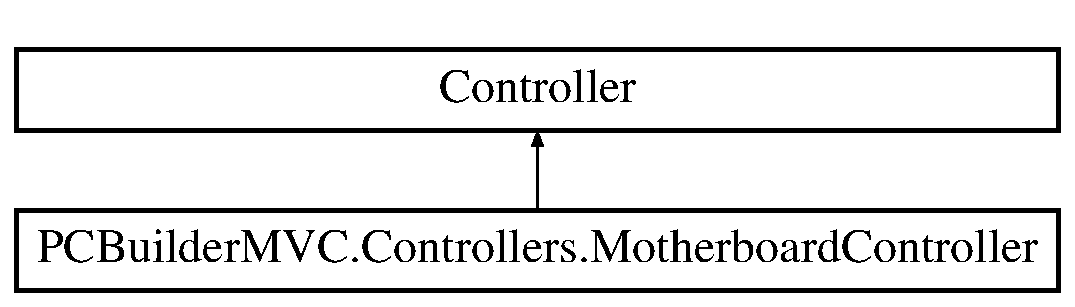
\includegraphics[height=2.000000cm]{class_p_c_builder_m_v_c_1_1_controllers_1_1_motherboard_controller}
\end{center}
\end{figure}
\subsection*{Public Member Functions}
\begin{DoxyCompactItemize}
\item 
Action\+Result {\bfseries Index} ()\hypertarget{class_p_c_builder_m_v_c_1_1_controllers_1_1_motherboard_controller_aa2a0f0e9dcb1ed08d282201866a6be89}{}\label{class_p_c_builder_m_v_c_1_1_controllers_1_1_motherboard_controller_aa2a0f0e9dcb1ed08d282201866a6be89}

\item 
Action\+Result {\bfseries Details} (int?id)\hypertarget{class_p_c_builder_m_v_c_1_1_controllers_1_1_motherboard_controller_a727538002744452af952b885559e9d8b}{}\label{class_p_c_builder_m_v_c_1_1_controllers_1_1_motherboard_controller_a727538002744452af952b885559e9d8b}

\item 
Action\+Result {\bfseries Create} ()\hypertarget{class_p_c_builder_m_v_c_1_1_controllers_1_1_motherboard_controller_abf7fa94ab1c69180e7976fb1cbf346bc}{}\label{class_p_c_builder_m_v_c_1_1_controllers_1_1_motherboard_controller_abf7fa94ab1c69180e7976fb1cbf346bc}

\item 
Action\+Result {\bfseries Create} (\mbox{[}Bind(Include=\char`\"{}Motherboard\+Id,Brand,Model,Socket,Chipset,Max\+Ram,Ram\+Type,Form\+Factor,Sata\+Ports,M2\+Slots,Power\+Phases,Fan\+Headers,Pcie16,Pcie8,Pcie4,Pcie1,Pci,Price\char`\"{})\mbox{]} Motherboard motherboard)\hypertarget{class_p_c_builder_m_v_c_1_1_controllers_1_1_motherboard_controller_a027a5f5735442481b44fd9b9bcde781e}{}\label{class_p_c_builder_m_v_c_1_1_controllers_1_1_motherboard_controller_a027a5f5735442481b44fd9b9bcde781e}

\item 
Action\+Result {\bfseries Edit} (int?id)\hypertarget{class_p_c_builder_m_v_c_1_1_controllers_1_1_motherboard_controller_adb4e93d677b42cbdfbb18eaecb4d86e2}{}\label{class_p_c_builder_m_v_c_1_1_controllers_1_1_motherboard_controller_adb4e93d677b42cbdfbb18eaecb4d86e2}

\item 
Action\+Result {\bfseries Edit} (\mbox{[}Bind(Include=\char`\"{}Motherboard\+Id,Brand,Model,Socket,Chipset,Max\+Ram,Ram\+Type,Form\+Factor,Sata\+Ports,M2\+Slots,Power\+Phases,Fan\+Headers,Pcie16,Pcie8,Pcie4,Pcie1,Pci,Price\char`\"{})\mbox{]} Motherboard motherboard)\hypertarget{class_p_c_builder_m_v_c_1_1_controllers_1_1_motherboard_controller_a05911fe623774ee2dcbd9bf1079aaf2e}{}\label{class_p_c_builder_m_v_c_1_1_controllers_1_1_motherboard_controller_a05911fe623774ee2dcbd9bf1079aaf2e}

\item 
Action\+Result {\bfseries Delete} (int?id)\hypertarget{class_p_c_builder_m_v_c_1_1_controllers_1_1_motherboard_controller_a03255789bef1157226db1f72785b2973}{}\label{class_p_c_builder_m_v_c_1_1_controllers_1_1_motherboard_controller_a03255789bef1157226db1f72785b2973}

\item 
Action\+Result {\bfseries Delete\+Confirmed} (int id)\hypertarget{class_p_c_builder_m_v_c_1_1_controllers_1_1_motherboard_controller_af944aebfcedf214c0182632f0082457b}{}\label{class_p_c_builder_m_v_c_1_1_controllers_1_1_motherboard_controller_af944aebfcedf214c0182632f0082457b}

\end{DoxyCompactItemize}
\subsection*{Protected Member Functions}
\begin{DoxyCompactItemize}
\item 
override void {\bfseries Dispose} (bool disposing)\hypertarget{class_p_c_builder_m_v_c_1_1_controllers_1_1_motherboard_controller_a1eedae183eaf739df0fda184eefb0233}{}\label{class_p_c_builder_m_v_c_1_1_controllers_1_1_motherboard_controller_a1eedae183eaf739df0fda184eefb0233}

\end{DoxyCompactItemize}
\subsection*{Private Attributes}
\begin{DoxyCompactItemize}
\item 
\hyperlink{class_p_c_builder_m_v_c_1_1_models_1_1_p_c_builder_entity_models}{P\+C\+Builder\+Entity\+Models} {\bfseries db} = new \hyperlink{class_p_c_builder_m_v_c_1_1_models_1_1_p_c_builder_entity_models}{P\+C\+Builder\+Entity\+Models}()\hypertarget{class_p_c_builder_m_v_c_1_1_controllers_1_1_motherboard_controller_aab8ffaf60c4310a2c64dfce1a4331e9a}{}\label{class_p_c_builder_m_v_c_1_1_controllers_1_1_motherboard_controller_aab8ffaf60c4310a2c64dfce1a4331e9a}

\end{DoxyCompactItemize}


\subsection{Detailed Description}
Motherboard controller class to handle Motherboard views interaction. 

\begin{DoxySeeAlso}{See also}
System.\+Web.\+Mvc.\+Controller


\end{DoxySeeAlso}


Definition at line 17 of file Motherboard\+Controller.\+cs.



The documentation for this class was generated from the following file\+:\begin{DoxyCompactItemize}
\item 
C\+:/\+Users/nh228u08/\+Desktop/\+Final\+Project/\+Final\+Project/\+P\+C\+Builder/\+P\+C\+Builder\+M\+V\+C/\+Controllers/Motherboard\+Controller.\+cs\end{DoxyCompactItemize}

\hypertarget{class_p_c_builder_m_v_c_1_1_mvc_application}{}\section{P\+C\+Builder\+M\+V\+C.\+Mvc\+Application Class Reference}
\label{class_p_c_builder_m_v_c_1_1_mvc_application}\index{P\+C\+Builder\+M\+V\+C.\+Mvc\+Application@{P\+C\+Builder\+M\+V\+C.\+Mvc\+Application}}


Global settings for M\+VC application.  


Inheritance diagram for P\+C\+Builder\+M\+V\+C.\+Mvc\+Application\+:\begin{figure}[H]
\begin{center}
\leavevmode
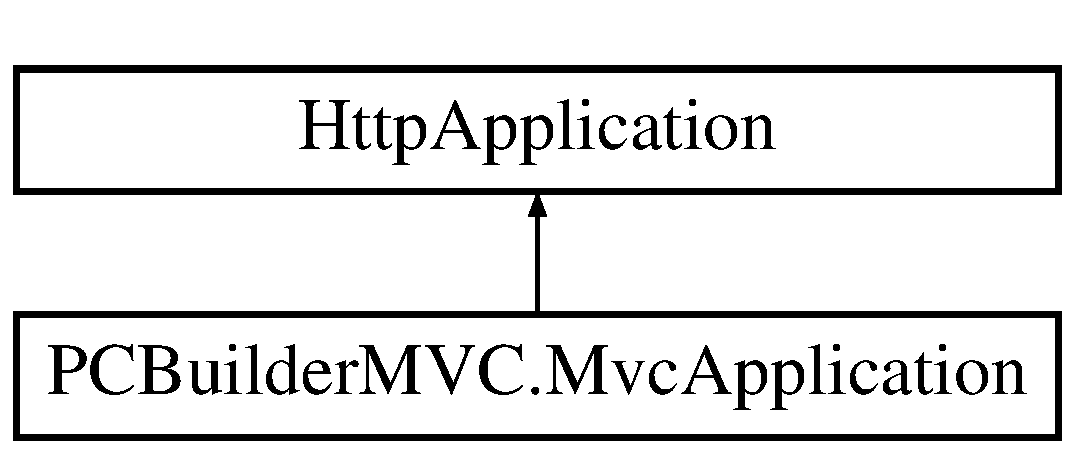
\includegraphics[height=2.000000cm]{class_p_c_builder_m_v_c_1_1_mvc_application}
\end{center}
\end{figure}
\subsection*{Protected Member Functions}
\begin{DoxyCompactItemize}
\item 
void {\bfseries Application\+\_\+\+Start} ()\hypertarget{class_p_c_builder_m_v_c_1_1_mvc_application_a79dbe3343b39de1768ebf8c9279ed6e7}{}\label{class_p_c_builder_m_v_c_1_1_mvc_application_a79dbe3343b39de1768ebf8c9279ed6e7}

\end{DoxyCompactItemize}


\subsection{Detailed Description}
Global settings for M\+VC application. 

\begin{DoxySeeAlso}{See also}
System.\+Web.\+Http\+Application


\end{DoxySeeAlso}


Definition at line 17 of file Global.\+asax.\+cs.



The documentation for this class was generated from the following file\+:\begin{DoxyCompactItemize}
\item 
C\+:/\+Users/nh228u08/\+Desktop/\+Final\+Project/\+Final\+Project/\+P\+C\+Builder/\+P\+C\+Builder\+M\+V\+C/Global.\+asax.\+cs\end{DoxyCompactItemize}

\hypertarget{class_business_objects_1_1_optical}{}\section{Business\+Objects.\+Optical Class Reference}
\label{class_business_objects_1_1_optical}\index{Business\+Objects.\+Optical@{Business\+Objects.\+Optical}}


\hyperlink{class_business_objects_1_1_optical}{Optical} object to hold necessary data on the optical drive  


\subsection*{Public Member Functions}
\begin{DoxyCompactItemize}
\item 
\hyperlink{class_business_objects_1_1_optical_a81db21dd419123fe11893f988facd077}{Optical} ()
\begin{DoxyCompactList}\small\item\em Initializes a new instance of the \hyperlink{class_business_objects_1_1_optical}{Optical} class. \end{DoxyCompactList}\item 
\hyperlink{class_business_objects_1_1_optical_a85e001030041386047f105975754144d}{Optical} (int optical\+Id, string brand, string model, string optical\+Type, decimal price)
\begin{DoxyCompactList}\small\item\em Initializes a new instance of the \hyperlink{class_business_objects_1_1_optical}{Optical} class. \end{DoxyCompactList}\end{DoxyCompactItemize}
\subsection*{Properties}
\begin{DoxyCompactItemize}
\item 
int {\bfseries Optical\+Id}\hspace{0.3cm}{\ttfamily  \mbox{[}get, set\mbox{]}}\hypertarget{class_business_objects_1_1_optical_adfb18e4b3a7a16fc1cad290e29a706a0}{}\label{class_business_objects_1_1_optical_adfb18e4b3a7a16fc1cad290e29a706a0}

\item 
string {\bfseries Brand}\hspace{0.3cm}{\ttfamily  \mbox{[}get, set\mbox{]}}\hypertarget{class_business_objects_1_1_optical_a39ba9566ba93a2d8e31ed1bfda850608}{}\label{class_business_objects_1_1_optical_a39ba9566ba93a2d8e31ed1bfda850608}

\item 
string {\bfseries Model}\hspace{0.3cm}{\ttfamily  \mbox{[}get, set\mbox{]}}\hypertarget{class_business_objects_1_1_optical_ad4f96eedb36b6e8d0bb0a757d8c2f162}{}\label{class_business_objects_1_1_optical_ad4f96eedb36b6e8d0bb0a757d8c2f162}

\item 
string {\bfseries Optical\+Type}\hspace{0.3cm}{\ttfamily  \mbox{[}get, set\mbox{]}}\hypertarget{class_business_objects_1_1_optical_afecc0495ac20fffeb10d11edcff6c3b6}{}\label{class_business_objects_1_1_optical_afecc0495ac20fffeb10d11edcff6c3b6}

\item 
decimal {\bfseries Price}\hspace{0.3cm}{\ttfamily  \mbox{[}get, set\mbox{]}}\hypertarget{class_business_objects_1_1_optical_a3913208c58242f22d7aaa48fd0d3a54d}{}\label{class_business_objects_1_1_optical_a3913208c58242f22d7aaa48fd0d3a54d}

\end{DoxyCompactItemize}


\subsection{Detailed Description}
\hyperlink{class_business_objects_1_1_optical}{Optical} object to hold necessary data on the optical drive 



Definition at line 17 of file Optical.\+cs.



\subsection{Constructor \& Destructor Documentation}
\index{Business\+Objects\+::\+Optical@{Business\+Objects\+::\+Optical}!Optical@{Optical}}
\index{Optical@{Optical}!Business\+Objects\+::\+Optical@{Business\+Objects\+::\+Optical}}
\subsubsection[{\texorpdfstring{Optical()}{Optical()}}]{\setlength{\rightskip}{0pt plus 5cm}Business\+Objects.\+Optical.\+Optical (
\begin{DoxyParamCaption}
{}
\end{DoxyParamCaption}
)}\hypertarget{class_business_objects_1_1_optical_a81db21dd419123fe11893f988facd077}{}\label{class_business_objects_1_1_optical_a81db21dd419123fe11893f988facd077}


Initializes a new instance of the \hyperlink{class_business_objects_1_1_optical}{Optical} class. 



Definition at line 28 of file Optical.\+cs.

\index{Business\+Objects\+::\+Optical@{Business\+Objects\+::\+Optical}!Optical@{Optical}}
\index{Optical@{Optical}!Business\+Objects\+::\+Optical@{Business\+Objects\+::\+Optical}}
\subsubsection[{\texorpdfstring{Optical(int optical\+Id, string brand, string model, string optical\+Type, decimal price)}{Optical(int opticalId, string brand, string model, string opticalType, decimal price)}}]{\setlength{\rightskip}{0pt plus 5cm}Business\+Objects.\+Optical.\+Optical (
\begin{DoxyParamCaption}
\item[{int}]{optical\+Id, }
\item[{string}]{brand, }
\item[{string}]{model, }
\item[{string}]{optical\+Type, }
\item[{decimal}]{price}
\end{DoxyParamCaption}
)}\hypertarget{class_business_objects_1_1_optical_a85e001030041386047f105975754144d}{}\label{class_business_objects_1_1_optical_a85e001030041386047f105975754144d}


Initializes a new instance of the \hyperlink{class_business_objects_1_1_optical}{Optical} class. 


\begin{DoxyParams}{Parameters}
{\em optical\+Id} & The optical identifier.\\
\hline
{\em brand} & The brand.\\
\hline
{\em model} & The model.\\
\hline
{\em optical\+Type} & Type of the optical drive.\\
\hline
{\em price} & The price.\\
\hline
\end{DoxyParams}


Definition at line 38 of file Optical.\+cs.



The documentation for this class was generated from the following file\+:\begin{DoxyCompactItemize}
\item 
C\+:/\+Users/nh228u08/\+Desktop/\+Final\+Project/\+Final\+Project/\+P\+C\+Builder/\+Business\+Objects/Optical.\+cs\end{DoxyCompactItemize}

\hypertarget{class_p_c_builder_m_v_c_1_1_models_1_1_optical}{}\section{P\+C\+Builder\+M\+V\+C.\+Models.\+Optical Class Reference}
\label{class_p_c_builder_m_v_c_1_1_models_1_1_optical}\index{P\+C\+Builder\+M\+V\+C.\+Models.\+Optical@{P\+C\+Builder\+M\+V\+C.\+Models.\+Optical}}


\hyperlink{class_p_c_builder_m_v_c_1_1_models_1_1_optical}{Optical} view model class.  


\subsection*{Properties}
\begin{DoxyCompactItemize}
\item 
int {\bfseries Optical\+Id}\hspace{0.3cm}{\ttfamily  \mbox{[}get, set\mbox{]}}\hypertarget{class_p_c_builder_m_v_c_1_1_models_1_1_optical_ad8f51257139f512f0ec6ad54fca96905}{}\label{class_p_c_builder_m_v_c_1_1_models_1_1_optical_ad8f51257139f512f0ec6ad54fca96905}

\item 
string {\bfseries Brand}\hspace{0.3cm}{\ttfamily  \mbox{[}get, set\mbox{]}}\hypertarget{class_p_c_builder_m_v_c_1_1_models_1_1_optical_a1b25c8c270d28d22aaa6d48644c57962}{}\label{class_p_c_builder_m_v_c_1_1_models_1_1_optical_a1b25c8c270d28d22aaa6d48644c57962}

\item 
string {\bfseries Model}\hspace{0.3cm}{\ttfamily  \mbox{[}get, set\mbox{]}}\hypertarget{class_p_c_builder_m_v_c_1_1_models_1_1_optical_a0529bf610b4aaa363b423caf26200c10}{}\label{class_p_c_builder_m_v_c_1_1_models_1_1_optical_a0529bf610b4aaa363b423caf26200c10}

\item 
string {\bfseries Optical\+Type}\hspace{0.3cm}{\ttfamily  \mbox{[}get, set\mbox{]}}\hypertarget{class_p_c_builder_m_v_c_1_1_models_1_1_optical_a8e452e1102a79129f77286b425bd780a}{}\label{class_p_c_builder_m_v_c_1_1_models_1_1_optical_a8e452e1102a79129f77286b425bd780a}

\item 
decimal {\bfseries Price}\hspace{0.3cm}{\ttfamily  \mbox{[}get, set\mbox{]}}\hypertarget{class_p_c_builder_m_v_c_1_1_models_1_1_optical_a70c467d88703603c376033c4d4058dc0}{}\label{class_p_c_builder_m_v_c_1_1_models_1_1_optical_a70c467d88703603c376033c4d4058dc0}

\end{DoxyCompactItemize}


\subsection{Detailed Description}
\hyperlink{class_p_c_builder_m_v_c_1_1_models_1_1_optical}{Optical} view model class. 



Definition at line 13 of file Optical.\+cs.



The documentation for this class was generated from the following file\+:\begin{DoxyCompactItemize}
\item 
C\+:/\+Users/nh228u08/\+Desktop/\+Final\+Project/\+Final\+Project/\+P\+C\+Builder/\+P\+C\+Builder\+M\+V\+C/\+Models/Optical.\+cs\end{DoxyCompactItemize}

\hypertarget{class_data_access_1_1_optical_accessor}{}\section{Data\+Access.\+Optical\+Accessor Class Reference}
\label{class_data_access_1_1_optical_accessor}\index{Data\+Access.\+Optical\+Accessor@{Data\+Access.\+Optical\+Accessor}}


Optical accessor to communicate with database on Optical drive objects.  


\subsection*{Static Public Member Functions}
\begin{DoxyCompactItemize}
\item 
static \hyperlink{class_business_objects_1_1_optical}{Optical} \hyperlink{class_data_access_1_1_optical_accessor_ac26fe61270034ab1ca7d39cc898758ad}{Retrieve\+Optical\+By\+Name} (string name)
\begin{DoxyCompactList}\small\item\em Retrieves optical drive by name. \end{DoxyCompactList}\item 
static List$<$ \hyperlink{class_business_objects_1_1_optical}{Optical} $>$ \hyperlink{class_data_access_1_1_optical_accessor_aec2da606590647ae3e6c6b80e6f920f2}{Retrieve\+Opticals\+By\+Type} (string type)
\begin{DoxyCompactList}\small\item\em Retrieves optical drives by type. \end{DoxyCompactList}\item 
static int \hyperlink{class_data_access_1_1_optical_accessor_aa2e6060824ca3ba994c360fc6918f3d4}{Insert\+Optical} (\hyperlink{class_business_objects_1_1_optical}{Optical} optical)
\begin{DoxyCompactList}\small\item\em Inserts a new optical drive. \end{DoxyCompactList}\end{DoxyCompactItemize}


\subsection{Detailed Description}
Optical accessor to communicate with database on Optical drive objects. 



Definition at line 15 of file Optical\+Accessor.\+cs.



\subsection{Member Function Documentation}
\index{Data\+Access\+::\+Optical\+Accessor@{Data\+Access\+::\+Optical\+Accessor}!Insert\+Optical@{Insert\+Optical}}
\index{Insert\+Optical@{Insert\+Optical}!Data\+Access\+::\+Optical\+Accessor@{Data\+Access\+::\+Optical\+Accessor}}
\subsubsection[{\texorpdfstring{Insert\+Optical(\+Optical optical)}{InsertOptical(Optical optical)}}]{\setlength{\rightskip}{0pt plus 5cm}static int Data\+Access.\+Optical\+Accessor.\+Insert\+Optical (
\begin{DoxyParamCaption}
\item[{{\bf Optical}}]{optical}
\end{DoxyParamCaption}
)\hspace{0.3cm}{\ttfamily [static]}}\hypertarget{class_data_access_1_1_optical_accessor_aa2e6060824ca3ba994c360fc6918f3d4}{}\label{class_data_access_1_1_optical_accessor_aa2e6060824ca3ba994c360fc6918f3d4}


Inserts a new optical drive. 


\begin{DoxyParams}{Parameters}
{\em optical} & The optical.\\
\hline
\end{DoxyParams}
\begin{DoxyReturn}{Returns}
Count of rows affected.
\end{DoxyReturn}


Definition at line 121 of file Optical\+Accessor.\+cs.

\index{Data\+Access\+::\+Optical\+Accessor@{Data\+Access\+::\+Optical\+Accessor}!Retrieve\+Optical\+By\+Name@{Retrieve\+Optical\+By\+Name}}
\index{Retrieve\+Optical\+By\+Name@{Retrieve\+Optical\+By\+Name}!Data\+Access\+::\+Optical\+Accessor@{Data\+Access\+::\+Optical\+Accessor}}
\subsubsection[{\texorpdfstring{Retrieve\+Optical\+By\+Name(string name)}{RetrieveOpticalByName(string name)}}]{\setlength{\rightskip}{0pt plus 5cm}static {\bf Optical} Data\+Access.\+Optical\+Accessor.\+Retrieve\+Optical\+By\+Name (
\begin{DoxyParamCaption}
\item[{string}]{name}
\end{DoxyParamCaption}
)\hspace{0.3cm}{\ttfamily [static]}}\hypertarget{class_data_access_1_1_optical_accessor_ac26fe61270034ab1ca7d39cc898758ad}{}\label{class_data_access_1_1_optical_accessor_ac26fe61270034ab1ca7d39cc898758ad}


Retrieves optical drive by name. 


\begin{DoxyParams}{Parameters}
{\em name} & The name.\\
\hline
\end{DoxyParams}
\begin{DoxyReturn}{Returns}
Optical drive object
\end{DoxyReturn}

\begin{DoxyExceptions}{Exceptions}
{\em System.\+Application\+Exception} & Data not found\\
\hline
\end{DoxyExceptions}


Definition at line 23 of file Optical\+Accessor.\+cs.

\index{Data\+Access\+::\+Optical\+Accessor@{Data\+Access\+::\+Optical\+Accessor}!Retrieve\+Opticals\+By\+Type@{Retrieve\+Opticals\+By\+Type}}
\index{Retrieve\+Opticals\+By\+Type@{Retrieve\+Opticals\+By\+Type}!Data\+Access\+::\+Optical\+Accessor@{Data\+Access\+::\+Optical\+Accessor}}
\subsubsection[{\texorpdfstring{Retrieve\+Opticals\+By\+Type(string type)}{RetrieveOpticalsByType(string type)}}]{\setlength{\rightskip}{0pt plus 5cm}static List$<${\bf Optical}$>$ Data\+Access.\+Optical\+Accessor.\+Retrieve\+Opticals\+By\+Type (
\begin{DoxyParamCaption}
\item[{string}]{type}
\end{DoxyParamCaption}
)\hspace{0.3cm}{\ttfamily [static]}}\hypertarget{class_data_access_1_1_optical_accessor_aec2da606590647ae3e6c6b80e6f920f2}{}\label{class_data_access_1_1_optical_accessor_aec2da606590647ae3e6c6b80e6f920f2}


Retrieves optical drives by type. 


\begin{DoxyParams}{Parameters}
{\em type} & The type.\\
\hline
\end{DoxyParams}
\begin{DoxyReturn}{Returns}
List of optical drives.
\end{DoxyReturn}

\begin{DoxyExceptions}{Exceptions}
{\em System.\+Application\+Exception} & Data not found\\
\hline
\end{DoxyExceptions}


Definition at line 72 of file Optical\+Accessor.\+cs.



The documentation for this class was generated from the following file\+:\begin{DoxyCompactItemize}
\item 
C\+:/\+Users/nh228u08/\+Desktop/\+Final\+Project/\+Final\+Project/\+P\+C\+Builder/\+Data\+Access/Optical\+Accessor.\+cs\end{DoxyCompactItemize}

\hypertarget{class_p_c_builder_m_v_c_1_1_controllers_1_1_optical_controller}{}\section{P\+C\+Builder\+M\+V\+C.\+Controllers.\+Optical\+Controller Class Reference}
\label{class_p_c_builder_m_v_c_1_1_controllers_1_1_optical_controller}\index{P\+C\+Builder\+M\+V\+C.\+Controllers.\+Optical\+Controller@{P\+C\+Builder\+M\+V\+C.\+Controllers.\+Optical\+Controller}}


Optical drive controller class to handle Optical views interaction.  


Inheritance diagram for P\+C\+Builder\+M\+V\+C.\+Controllers.\+Optical\+Controller\+:\begin{figure}[H]
\begin{center}
\leavevmode
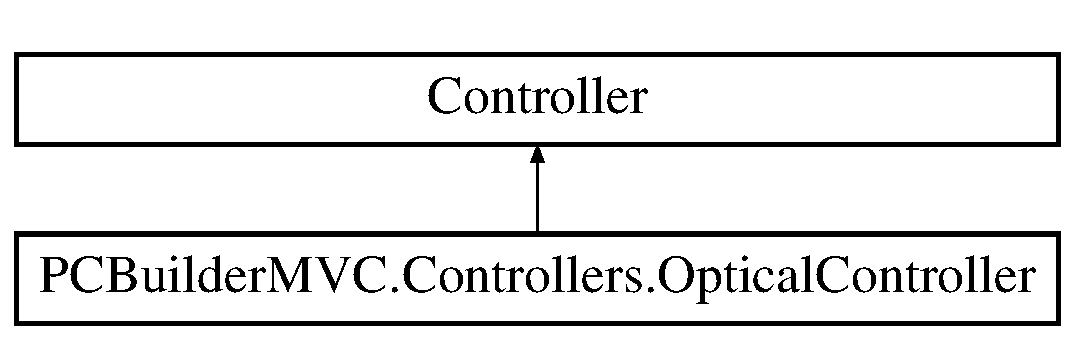
\includegraphics[height=2.000000cm]{class_p_c_builder_m_v_c_1_1_controllers_1_1_optical_controller}
\end{center}
\end{figure}
\subsection*{Public Member Functions}
\begin{DoxyCompactItemize}
\item 
Action\+Result {\bfseries Index} ()\hypertarget{class_p_c_builder_m_v_c_1_1_controllers_1_1_optical_controller_a19d91c5c0eb4c6db44a9b52e49caa15c}{}\label{class_p_c_builder_m_v_c_1_1_controllers_1_1_optical_controller_a19d91c5c0eb4c6db44a9b52e49caa15c}

\item 
Action\+Result {\bfseries Details} (int?id)\hypertarget{class_p_c_builder_m_v_c_1_1_controllers_1_1_optical_controller_a451e9a21abefe7878228c4af97e42fb4}{}\label{class_p_c_builder_m_v_c_1_1_controllers_1_1_optical_controller_a451e9a21abefe7878228c4af97e42fb4}

\item 
Action\+Result {\bfseries Create} ()\hypertarget{class_p_c_builder_m_v_c_1_1_controllers_1_1_optical_controller_af5abe48aa5f880e392a1578c43e533a7}{}\label{class_p_c_builder_m_v_c_1_1_controllers_1_1_optical_controller_af5abe48aa5f880e392a1578c43e533a7}

\item 
Action\+Result {\bfseries Create} (\mbox{[}Bind(Include=\char`\"{}Optical\+Id,Brand,Model,Optical\+Type,Price\char`\"{})\mbox{]} Optical optical)\hypertarget{class_p_c_builder_m_v_c_1_1_controllers_1_1_optical_controller_a003bcc62793607ef4d4a79a7e821abcc}{}\label{class_p_c_builder_m_v_c_1_1_controllers_1_1_optical_controller_a003bcc62793607ef4d4a79a7e821abcc}

\item 
Action\+Result {\bfseries Edit} (int?id)\hypertarget{class_p_c_builder_m_v_c_1_1_controllers_1_1_optical_controller_ad97768ce3483ae9d4407f55ac1825221}{}\label{class_p_c_builder_m_v_c_1_1_controllers_1_1_optical_controller_ad97768ce3483ae9d4407f55ac1825221}

\item 
Action\+Result {\bfseries Edit} (\mbox{[}Bind(Include=\char`\"{}Optical\+Id,Brand,Model,Optical\+Type,Price\char`\"{})\mbox{]} Optical optical)\hypertarget{class_p_c_builder_m_v_c_1_1_controllers_1_1_optical_controller_a8a2ad0474ec18caed739167e1b535630}{}\label{class_p_c_builder_m_v_c_1_1_controllers_1_1_optical_controller_a8a2ad0474ec18caed739167e1b535630}

\item 
Action\+Result {\bfseries Delete} (int?id)\hypertarget{class_p_c_builder_m_v_c_1_1_controllers_1_1_optical_controller_a3ec1c51763dc146925d897e15fb3f33f}{}\label{class_p_c_builder_m_v_c_1_1_controllers_1_1_optical_controller_a3ec1c51763dc146925d897e15fb3f33f}

\item 
Action\+Result {\bfseries Delete\+Confirmed} (int id)\hypertarget{class_p_c_builder_m_v_c_1_1_controllers_1_1_optical_controller_aa88c8083a1bb937c87dc99359495b4d3}{}\label{class_p_c_builder_m_v_c_1_1_controllers_1_1_optical_controller_aa88c8083a1bb937c87dc99359495b4d3}

\end{DoxyCompactItemize}
\subsection*{Protected Member Functions}
\begin{DoxyCompactItemize}
\item 
override void {\bfseries Dispose} (bool disposing)\hypertarget{class_p_c_builder_m_v_c_1_1_controllers_1_1_optical_controller_a25e4700610f3e58e07a3ef2cfbe12330}{}\label{class_p_c_builder_m_v_c_1_1_controllers_1_1_optical_controller_a25e4700610f3e58e07a3ef2cfbe12330}

\end{DoxyCompactItemize}
\subsection*{Private Attributes}
\begin{DoxyCompactItemize}
\item 
\hyperlink{class_p_c_builder_m_v_c_1_1_models_1_1_p_c_builder_entity_models}{P\+C\+Builder\+Entity\+Models} {\bfseries db} = new \hyperlink{class_p_c_builder_m_v_c_1_1_models_1_1_p_c_builder_entity_models}{P\+C\+Builder\+Entity\+Models}()\hypertarget{class_p_c_builder_m_v_c_1_1_controllers_1_1_optical_controller_a5391c12ed8f836eac784c9247511a411}{}\label{class_p_c_builder_m_v_c_1_1_controllers_1_1_optical_controller_a5391c12ed8f836eac784c9247511a411}

\end{DoxyCompactItemize}


\subsection{Detailed Description}
Optical drive controller class to handle Optical views interaction. 

\begin{DoxySeeAlso}{See also}
System.\+Web.\+Mvc.\+Controller


\end{DoxySeeAlso}


Definition at line 17 of file Optical\+Controller.\+cs.



The documentation for this class was generated from the following file\+:\begin{DoxyCompactItemize}
\item 
C\+:/\+Users/nh228u08/\+Desktop/\+Final\+Project/\+Final\+Project/\+P\+C\+Builder/\+P\+C\+Builder\+M\+V\+C/\+Controllers/Optical\+Controller.\+cs\end{DoxyCompactItemize}

\hypertarget{class_p_c_builder_m_v_c_1_1_models_1_1_p_c_builder_entity_models}{}\section{P\+C\+Builder\+M\+V\+C.\+Models.\+P\+C\+Builder\+Entity\+Models Class Reference}
\label{class_p_c_builder_m_v_c_1_1_models_1_1_p_c_builder_entity_models}\index{P\+C\+Builder\+M\+V\+C.\+Models.\+P\+C\+Builder\+Entity\+Models@{P\+C\+Builder\+M\+V\+C.\+Models.\+P\+C\+Builder\+Entity\+Models}}


P\+C\+Builder Entity Framework \hyperlink{namespace_p_c_builder_m_v_c_1_1_models}{Models} view model class.  


Inheritance diagram for P\+C\+Builder\+M\+V\+C.\+Models.\+P\+C\+Builder\+Entity\+Models\+:\begin{figure}[H]
\begin{center}
\leavevmode
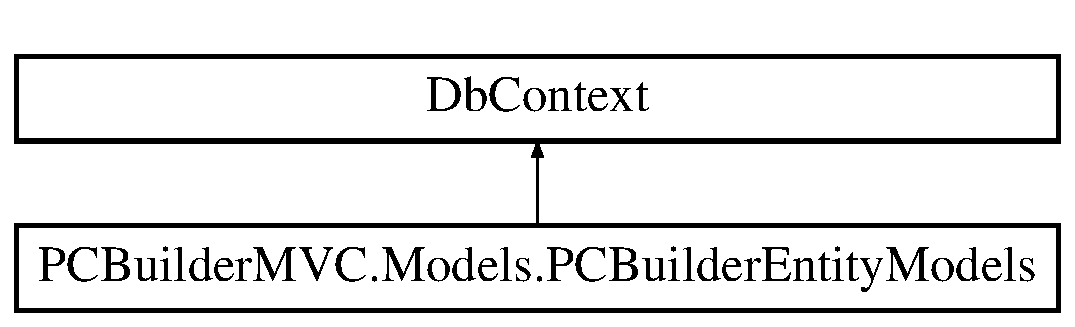
\includegraphics[height=2.000000cm]{class_p_c_builder_m_v_c_1_1_models_1_1_p_c_builder_entity_models}
\end{center}
\end{figure}
\subsection*{Protected Member Functions}
\begin{DoxyCompactItemize}
\item 
override void {\bfseries On\+Model\+Creating} (Db\+Model\+Builder model\+Builder)\hypertarget{class_p_c_builder_m_v_c_1_1_models_1_1_p_c_builder_entity_models_a6f1980dd854d63223c69a6b1fd948f74}{}\label{class_p_c_builder_m_v_c_1_1_models_1_1_p_c_builder_entity_models_a6f1980dd854d63223c69a6b1fd948f74}

\end{DoxyCompactItemize}
\subsection*{Properties}
\begin{DoxyCompactItemize}
\item 
virtual Db\+Set$<$ \hyperlink{class_p_c_builder_m_v_c_1_1_models_1_1_c_p_u}{C\+PU} $>$ {\bfseries C\+P\+Us}\hspace{0.3cm}{\ttfamily  \mbox{[}get, set\mbox{]}}\hypertarget{class_p_c_builder_m_v_c_1_1_models_1_1_p_c_builder_entity_models_a9412e2ad51d1271e2e22a72452fd2b89}{}\label{class_p_c_builder_m_v_c_1_1_models_1_1_p_c_builder_entity_models_a9412e2ad51d1271e2e22a72452fd2b89}

\item 
virtual Db\+Set$<$ \hyperlink{class_p_c_builder_m_v_c_1_1_models_1_1_g_p_u}{G\+PU} $>$ {\bfseries G\+P\+Us}\hspace{0.3cm}{\ttfamily  \mbox{[}get, set\mbox{]}}\hypertarget{class_p_c_builder_m_v_c_1_1_models_1_1_p_c_builder_entity_models_aaa8038351676c90b1cf5adde3466d9d3}{}\label{class_p_c_builder_m_v_c_1_1_models_1_1_p_c_builder_entity_models_aaa8038351676c90b1cf5adde3466d9d3}

\item 
virtual Db\+Set$<$ \hyperlink{class_p_c_builder_m_v_c_1_1_models_1_1_motherboard}{Motherboard} $>$ {\bfseries Motherboards}\hspace{0.3cm}{\ttfamily  \mbox{[}get, set\mbox{]}}\hypertarget{class_p_c_builder_m_v_c_1_1_models_1_1_p_c_builder_entity_models_a8d4169fcc124efe24a0e41c727d0497e}{}\label{class_p_c_builder_m_v_c_1_1_models_1_1_p_c_builder_entity_models_a8d4169fcc124efe24a0e41c727d0497e}

\item 
virtual Db\+Set$<$ \hyperlink{class_p_c_builder_m_v_c_1_1_models_1_1_optical}{Optical} $>$ {\bfseries Opticals}\hspace{0.3cm}{\ttfamily  \mbox{[}get, set\mbox{]}}\hypertarget{class_p_c_builder_m_v_c_1_1_models_1_1_p_c_builder_entity_models_ac0a93bd467639e52e02051e12bfa44e5}{}\label{class_p_c_builder_m_v_c_1_1_models_1_1_p_c_builder_entity_models_ac0a93bd467639e52e02051e12bfa44e5}

\item 
virtual Db\+Set$<$ \hyperlink{class_p_c_builder_m_v_c_1_1_models_1_1_p_s_u}{P\+SU} $>$ {\bfseries P\+S\+Us}\hspace{0.3cm}{\ttfamily  \mbox{[}get, set\mbox{]}}\hypertarget{class_p_c_builder_m_v_c_1_1_models_1_1_p_c_builder_entity_models_a0a5f731f0bcf9b1cdfb6865ecde4c08b}{}\label{class_p_c_builder_m_v_c_1_1_models_1_1_p_c_builder_entity_models_a0a5f731f0bcf9b1cdfb6865ecde4c08b}

\item 
virtual Db\+Set$<$ \hyperlink{class_p_c_builder_m_v_c_1_1_models_1_1_r_a_m}{R\+AM} $>$ {\bfseries R\+A\+Ms}\hspace{0.3cm}{\ttfamily  \mbox{[}get, set\mbox{]}}\hypertarget{class_p_c_builder_m_v_c_1_1_models_1_1_p_c_builder_entity_models_aa58a925658f5db1a2451cdb6a0d57949}{}\label{class_p_c_builder_m_v_c_1_1_models_1_1_p_c_builder_entity_models_aa58a925658f5db1a2451cdb6a0d57949}

\item 
virtual Db\+Set$<$ \hyperlink{class_p_c_builder_m_v_c_1_1_models_1_1_role}{Role} $>$ {\bfseries Roles}\hspace{0.3cm}{\ttfamily  \mbox{[}get, set\mbox{]}}\hypertarget{class_p_c_builder_m_v_c_1_1_models_1_1_p_c_builder_entity_models_ab650b1da81b3077e41abe4ef3e0777cb}{}\label{class_p_c_builder_m_v_c_1_1_models_1_1_p_c_builder_entity_models_ab650b1da81b3077e41abe4ef3e0777cb}

\item 
virtual Db\+Set$<$ \hyperlink{class_p_c_builder_m_v_c_1_1_models_1_1_storage}{Storage} $>$ {\bfseries Storages}\hspace{0.3cm}{\ttfamily  \mbox{[}get, set\mbox{]}}\hypertarget{class_p_c_builder_m_v_c_1_1_models_1_1_p_c_builder_entity_models_a79853744639305e4b275548629834558}{}\label{class_p_c_builder_m_v_c_1_1_models_1_1_p_c_builder_entity_models_a79853744639305e4b275548629834558}

\item 
virtual Db\+Set$<$ \hyperlink{class_p_c_builder_m_v_c_1_1_models_1_1_user}{User} $>$ {\bfseries Users}\hspace{0.3cm}{\ttfamily  \mbox{[}get, set\mbox{]}}\hypertarget{class_p_c_builder_m_v_c_1_1_models_1_1_p_c_builder_entity_models_a78925feeeef3b89318953daddeedc6ab}{}\label{class_p_c_builder_m_v_c_1_1_models_1_1_p_c_builder_entity_models_a78925feeeef3b89318953daddeedc6ab}

\item 
System.\+Data.\+Entity.\+Db\+Set$<$ \hyperlink{class_p_c_builder_m_v_c_1_1_models_1_1_questionnaire_view_model}{P\+C\+Builder\+M\+V\+C.\+Models.\+Questionnaire\+View\+Model} $>$ {\bfseries Questionnaire\+View\+Models}\hspace{0.3cm}{\ttfamily  \mbox{[}get, set\mbox{]}}\hypertarget{class_p_c_builder_m_v_c_1_1_models_1_1_p_c_builder_entity_models_ada46bb5ef5120abffefa3ce38be5843a}{}\label{class_p_c_builder_m_v_c_1_1_models_1_1_p_c_builder_entity_models_ada46bb5ef5120abffefa3ce38be5843a}

\item 
System.\+Data.\+Entity.\+Db\+Set$<$ \hyperlink{class_p_c_builder_m_v_c_1_1_models_1_1_finalized_build_view_model}{P\+C\+Builder\+M\+V\+C.\+Models.\+Finalized\+Build\+View\+Model} $>$ {\bfseries Finalized\+Build\+View\+Models}\hspace{0.3cm}{\ttfamily  \mbox{[}get, set\mbox{]}}\hypertarget{class_p_c_builder_m_v_c_1_1_models_1_1_p_c_builder_entity_models_a6cb50b4dd2ce526459e7dc52381fc627}{}\label{class_p_c_builder_m_v_c_1_1_models_1_1_p_c_builder_entity_models_a6cb50b4dd2ce526459e7dc52381fc627}

\item 
System.\+Data.\+Entity.\+Db\+Set$<$ \hyperlink{class_p_c_builder_m_v_c_1_1_models_1_1_asp_net_user}{P\+C\+Builder\+M\+V\+C.\+Models.\+Asp\+Net\+User} $>$ {\bfseries Asp\+Net\+Users}\hspace{0.3cm}{\ttfamily  \mbox{[}get, set\mbox{]}}\hypertarget{class_p_c_builder_m_v_c_1_1_models_1_1_p_c_builder_entity_models_a4b38df58c1b0bb6500f88dbbd6b5e2d0}{}\label{class_p_c_builder_m_v_c_1_1_models_1_1_p_c_builder_entity_models_a4b38df58c1b0bb6500f88dbbd6b5e2d0}

\item 
System.\+Data.\+Entity.\+Db\+Set$<$ \hyperlink{class_p_c_builder_m_v_c_1_1_models_1_1_asp_net_role}{P\+C\+Builder\+M\+V\+C.\+Models.\+Asp\+Net\+Role} $>$ {\bfseries Asp\+Net\+Roles}\hspace{0.3cm}{\ttfamily  \mbox{[}get, set\mbox{]}}\hypertarget{class_p_c_builder_m_v_c_1_1_models_1_1_p_c_builder_entity_models_a89e01a79119dd60e1149e6be03f6cf81}{}\label{class_p_c_builder_m_v_c_1_1_models_1_1_p_c_builder_entity_models_a89e01a79119dd60e1149e6be03f6cf81}

\end{DoxyCompactItemize}


\subsection{Detailed Description}
P\+C\+Builder Entity Framework \hyperlink{namespace_p_c_builder_m_v_c_1_1_models}{Models} view model class. 

\begin{DoxySeeAlso}{See also}
System.\+Data.\+Entity.\+Db\+Context


\end{DoxySeeAlso}


Definition at line 12 of file P\+C\+Builder\+Entity\+Models.\+cs.



The documentation for this class was generated from the following file\+:\begin{DoxyCompactItemize}
\item 
C\+:/\+Users/nh228u08/\+Desktop/\+Final\+Project/\+Final\+Project/\+P\+C\+Builder/\+P\+C\+Builder\+M\+V\+C/\+Models/P\+C\+Builder\+Entity\+Models.\+cs\end{DoxyCompactItemize}

\hypertarget{class_business_objects_1_1_p_s_u}{}\section{Business\+Objects.\+P\+SU Class Reference}
\label{class_business_objects_1_1_p_s_u}\index{Business\+Objects.\+P\+SU@{Business\+Objects.\+P\+SU}}


\hyperlink{class_business_objects_1_1_p_s_u}{P\+SU} object to hold necessary data on the \hyperlink{class_business_objects_1_1_p_s_u}{P\+SU}.  


\subsection*{Public Member Functions}
\begin{DoxyCompactItemize}
\item 
\hyperlink{class_business_objects_1_1_p_s_u_a797da5110778eadc6ae1770b7b6fa1f7}{P\+SU} ()
\begin{DoxyCompactList}\small\item\em Initializes a new instance of the \hyperlink{class_business_objects_1_1_p_s_u}{P\+SU} class. \end{DoxyCompactList}\item 
\hyperlink{class_business_objects_1_1_p_s_u_ae552ae19d45745f5a7b3138e80309fd3}{P\+SU} (int psu\+Id, string brand, string model, int wattage, string efficiency, decimal price)
\begin{DoxyCompactList}\small\item\em Initializes a new instance of the \hyperlink{class_business_objects_1_1_p_s_u}{P\+SU} class. \end{DoxyCompactList}\end{DoxyCompactItemize}
\subsection*{Properties}
\begin{DoxyCompactItemize}
\item 
int {\bfseries Psu\+Id}\hspace{0.3cm}{\ttfamily  \mbox{[}get, set\mbox{]}}\hypertarget{class_business_objects_1_1_p_s_u_ab1c703d2846b1b7a0bd1c62f918aabef}{}\label{class_business_objects_1_1_p_s_u_ab1c703d2846b1b7a0bd1c62f918aabef}

\item 
string {\bfseries Brand}\hspace{0.3cm}{\ttfamily  \mbox{[}get, set\mbox{]}}\hypertarget{class_business_objects_1_1_p_s_u_a21529fd3e98dcae4c9b169d3324a083b}{}\label{class_business_objects_1_1_p_s_u_a21529fd3e98dcae4c9b169d3324a083b}

\item 
string {\bfseries Model}\hspace{0.3cm}{\ttfamily  \mbox{[}get, set\mbox{]}}\hypertarget{class_business_objects_1_1_p_s_u_a61151c4df983466da3f88f255bfab7b8}{}\label{class_business_objects_1_1_p_s_u_a61151c4df983466da3f88f255bfab7b8}

\item 
int {\bfseries Wattage}\hspace{0.3cm}{\ttfamily  \mbox{[}get, set\mbox{]}}\hypertarget{class_business_objects_1_1_p_s_u_a9daaba69d8ef52adeb86bc89d0aa6a4d}{}\label{class_business_objects_1_1_p_s_u_a9daaba69d8ef52adeb86bc89d0aa6a4d}

\item 
string {\bfseries Efficiency}\hspace{0.3cm}{\ttfamily  \mbox{[}get, set\mbox{]}}\hypertarget{class_business_objects_1_1_p_s_u_a10bfc5e78c2ef86a33b947dd1578aae2}{}\label{class_business_objects_1_1_p_s_u_a10bfc5e78c2ef86a33b947dd1578aae2}

\item 
decimal {\bfseries Price}\hspace{0.3cm}{\ttfamily  \mbox{[}get, set\mbox{]}}\hypertarget{class_business_objects_1_1_p_s_u_a9384364baec19b5b9205133831945c2e}{}\label{class_business_objects_1_1_p_s_u_a9384364baec19b5b9205133831945c2e}

\end{DoxyCompactItemize}


\subsection{Detailed Description}
\hyperlink{class_business_objects_1_1_p_s_u}{P\+SU} object to hold necessary data on the \hyperlink{class_business_objects_1_1_p_s_u}{P\+SU}. 



Definition at line 17 of file P\+S\+U.\+cs.



\subsection{Constructor \& Destructor Documentation}
\index{Business\+Objects\+::\+P\+SU@{Business\+Objects\+::\+P\+SU}!P\+SU@{P\+SU}}
\index{P\+SU@{P\+SU}!Business\+Objects\+::\+P\+SU@{Business\+Objects\+::\+P\+SU}}
\subsubsection[{\texorpdfstring{P\+S\+U()}{PSU()}}]{\setlength{\rightskip}{0pt plus 5cm}Business\+Objects.\+P\+S\+U.\+P\+SU (
\begin{DoxyParamCaption}
{}
\end{DoxyParamCaption}
)}\hypertarget{class_business_objects_1_1_p_s_u_a797da5110778eadc6ae1770b7b6fa1f7}{}\label{class_business_objects_1_1_p_s_u_a797da5110778eadc6ae1770b7b6fa1f7}


Initializes a new instance of the \hyperlink{class_business_objects_1_1_p_s_u}{P\+SU} class. 



Definition at line 29 of file P\+S\+U.\+cs.

\index{Business\+Objects\+::\+P\+SU@{Business\+Objects\+::\+P\+SU}!P\+SU@{P\+SU}}
\index{P\+SU@{P\+SU}!Business\+Objects\+::\+P\+SU@{Business\+Objects\+::\+P\+SU}}
\subsubsection[{\texorpdfstring{P\+S\+U(int psu\+Id, string brand, string model, int wattage, string efficiency, decimal price)}{PSU(int psuId, string brand, string model, int wattage, string efficiency, decimal price)}}]{\setlength{\rightskip}{0pt plus 5cm}Business\+Objects.\+P\+S\+U.\+P\+SU (
\begin{DoxyParamCaption}
\item[{int}]{psu\+Id, }
\item[{string}]{brand, }
\item[{string}]{model, }
\item[{int}]{wattage, }
\item[{string}]{efficiency, }
\item[{decimal}]{price}
\end{DoxyParamCaption}
)}\hypertarget{class_business_objects_1_1_p_s_u_ae552ae19d45745f5a7b3138e80309fd3}{}\label{class_business_objects_1_1_p_s_u_ae552ae19d45745f5a7b3138e80309fd3}


Initializes a new instance of the \hyperlink{class_business_objects_1_1_p_s_u}{P\+SU} class. 


\begin{DoxyParams}{Parameters}
{\em psu\+Id} & The psu identifier.\\
\hline
{\em brand} & The brand.\\
\hline
{\em model} & The model.\\
\hline
{\em wattage} & The wattage.\\
\hline
{\em efficiency} & The efficiency.\\
\hline
{\em price} & The price.\\
\hline
\end{DoxyParams}


Definition at line 40 of file P\+S\+U.\+cs.



The documentation for this class was generated from the following file\+:\begin{DoxyCompactItemize}
\item 
C\+:/\+Users/nh228u08/\+Desktop/\+Final\+Project/\+Final\+Project/\+P\+C\+Builder/\+Business\+Objects/P\+S\+U.\+cs\end{DoxyCompactItemize}

\hypertarget{class_p_c_builder_m_v_c_1_1_models_1_1_p_s_u}{}\section{P\+C\+Builder\+M\+V\+C.\+Models.\+P\+SU Class Reference}
\label{class_p_c_builder_m_v_c_1_1_models_1_1_p_s_u}\index{P\+C\+Builder\+M\+V\+C.\+Models.\+P\+SU@{P\+C\+Builder\+M\+V\+C.\+Models.\+P\+SU}}


\hyperlink{class_p_c_builder_m_v_c_1_1_models_1_1_p_s_u}{P\+SU} view model class.  


\subsection*{Properties}
\begin{DoxyCompactItemize}
\item 
int {\bfseries Psu\+Id}\hspace{0.3cm}{\ttfamily  \mbox{[}get, set\mbox{]}}\hypertarget{class_p_c_builder_m_v_c_1_1_models_1_1_p_s_u_a1aa8f13f4f65fac57188abd27fec6361}{}\label{class_p_c_builder_m_v_c_1_1_models_1_1_p_s_u_a1aa8f13f4f65fac57188abd27fec6361}

\item 
string {\bfseries Brand}\hspace{0.3cm}{\ttfamily  \mbox{[}get, set\mbox{]}}\hypertarget{class_p_c_builder_m_v_c_1_1_models_1_1_p_s_u_a6a4566057f3f1faa0a76b7523f6381b5}{}\label{class_p_c_builder_m_v_c_1_1_models_1_1_p_s_u_a6a4566057f3f1faa0a76b7523f6381b5}

\item 
string {\bfseries Model}\hspace{0.3cm}{\ttfamily  \mbox{[}get, set\mbox{]}}\hypertarget{class_p_c_builder_m_v_c_1_1_models_1_1_p_s_u_ad1ce3afa398e0d81611614408e3e504c}{}\label{class_p_c_builder_m_v_c_1_1_models_1_1_p_s_u_ad1ce3afa398e0d81611614408e3e504c}

\item 
int {\bfseries Wattage}\hspace{0.3cm}{\ttfamily  \mbox{[}get, set\mbox{]}}\hypertarget{class_p_c_builder_m_v_c_1_1_models_1_1_p_s_u_a1003235ba50a1a9cdce50d9e985db3d9}{}\label{class_p_c_builder_m_v_c_1_1_models_1_1_p_s_u_a1003235ba50a1a9cdce50d9e985db3d9}

\item 
string {\bfseries Efficiency}\hspace{0.3cm}{\ttfamily  \mbox{[}get, set\mbox{]}}\hypertarget{class_p_c_builder_m_v_c_1_1_models_1_1_p_s_u_a3a2bf09667c2d0c6b9c44de0f9464a73}{}\label{class_p_c_builder_m_v_c_1_1_models_1_1_p_s_u_a3a2bf09667c2d0c6b9c44de0f9464a73}

\item 
decimal {\bfseries Price}\hspace{0.3cm}{\ttfamily  \mbox{[}get, set\mbox{]}}\hypertarget{class_p_c_builder_m_v_c_1_1_models_1_1_p_s_u_af66a2e0cf50a961fe83f40c53692e78b}{}\label{class_p_c_builder_m_v_c_1_1_models_1_1_p_s_u_af66a2e0cf50a961fe83f40c53692e78b}

\end{DoxyCompactItemize}


\subsection{Detailed Description}
\hyperlink{class_p_c_builder_m_v_c_1_1_models_1_1_p_s_u}{P\+SU} view model class. 



Definition at line 13 of file P\+S\+U.\+cs.



The documentation for this class was generated from the following file\+:\begin{DoxyCompactItemize}
\item 
C\+:/\+Users/nh228u08/\+Desktop/\+Final\+Project/\+Final\+Project/\+P\+C\+Builder/\+P\+C\+Builder\+M\+V\+C/\+Models/P\+S\+U.\+cs\end{DoxyCompactItemize}

\hypertarget{class_data_access_1_1_p_s_u_accessor}{}\section{Data\+Access.\+P\+S\+U\+Accessor Class Reference}
\label{class_data_access_1_1_p_s_u_accessor}\index{Data\+Access.\+P\+S\+U\+Accessor@{Data\+Access.\+P\+S\+U\+Accessor}}


P\+SU accessor to communicate with database on P\+SU objects.  


\subsection*{Static Public Member Functions}
\begin{DoxyCompactItemize}
\item 
static \hyperlink{class_business_objects_1_1_p_s_u}{P\+SU} \hyperlink{class_data_access_1_1_p_s_u_accessor_a18a99912fcddb6255d3b36d74cdb4e57}{Retrieve\+P\+S\+U\+By\+Name} (string name)
\begin{DoxyCompactList}\small\item\em Retrieves a P\+SU by name. \end{DoxyCompactList}\item 
static List$<$ \hyperlink{class_business_objects_1_1_p_s_u}{P\+SU} $>$ \hyperlink{class_data_access_1_1_p_s_u_accessor_a83eb22b79d6bd8ab03b2bcf0ce8fe5ea}{Retrieve\+P\+S\+Us\+By\+Wattage} (string wattage)
\begin{DoxyCompactList}\small\item\em Retrieves P\+S\+Us by wattage. \end{DoxyCompactList}\item 
static int \hyperlink{class_data_access_1_1_p_s_u_accessor_a3285bd4b20ff99e005ef98f496f8d2dd}{Insert\+P\+SU} (\hyperlink{class_business_objects_1_1_p_s_u}{P\+SU} psu)
\begin{DoxyCompactList}\small\item\em Inserts a new P\+SU. \end{DoxyCompactList}\item 
static List$<$ \hyperlink{class_business_objects_1_1_p_s_u}{P\+SU} $>$ \hyperlink{class_data_access_1_1_p_s_u_accessor_a6f1192a9cf546dab42dab3d31c7c27e8}{Retrieve\+All\+P\+SU} ()
\begin{DoxyCompactList}\small\item\em Retrieves all P\+S\+Us. \end{DoxyCompactList}\end{DoxyCompactItemize}


\subsection{Detailed Description}
P\+SU accessor to communicate with database on P\+SU objects. 



Definition at line 15 of file P\+S\+U\+Accessor.\+cs.



\subsection{Member Function Documentation}
\index{Data\+Access\+::\+P\+S\+U\+Accessor@{Data\+Access\+::\+P\+S\+U\+Accessor}!Insert\+P\+SU@{Insert\+P\+SU}}
\index{Insert\+P\+SU@{Insert\+P\+SU}!Data\+Access\+::\+P\+S\+U\+Accessor@{Data\+Access\+::\+P\+S\+U\+Accessor}}
\subsubsection[{\texorpdfstring{Insert\+P\+S\+U(\+P\+S\+U psu)}{InsertPSU(PSU psu)}}]{\setlength{\rightskip}{0pt plus 5cm}static int Data\+Access.\+P\+S\+U\+Accessor.\+Insert\+P\+SU (
\begin{DoxyParamCaption}
\item[{{\bf P\+SU}}]{psu}
\end{DoxyParamCaption}
)\hspace{0.3cm}{\ttfamily [static]}}\hypertarget{class_data_access_1_1_p_s_u_accessor_a3285bd4b20ff99e005ef98f496f8d2dd}{}\label{class_data_access_1_1_p_s_u_accessor_a3285bd4b20ff99e005ef98f496f8d2dd}


Inserts a new P\+SU. 


\begin{DoxyParams}{Parameters}
{\em psu} & The psu.\\
\hline
\end{DoxyParams}
\begin{DoxyReturn}{Returns}
Count of rows affected.
\end{DoxyReturn}


Definition at line 123 of file P\+S\+U\+Accessor.\+cs.

\index{Data\+Access\+::\+P\+S\+U\+Accessor@{Data\+Access\+::\+P\+S\+U\+Accessor}!Retrieve\+All\+P\+SU@{Retrieve\+All\+P\+SU}}
\index{Retrieve\+All\+P\+SU@{Retrieve\+All\+P\+SU}!Data\+Access\+::\+P\+S\+U\+Accessor@{Data\+Access\+::\+P\+S\+U\+Accessor}}
\subsubsection[{\texorpdfstring{Retrieve\+All\+P\+S\+U()}{RetrieveAllPSU()}}]{\setlength{\rightskip}{0pt plus 5cm}static List$<${\bf P\+SU}$>$ Data\+Access.\+P\+S\+U\+Accessor.\+Retrieve\+All\+P\+SU (
\begin{DoxyParamCaption}
{}
\end{DoxyParamCaption}
)\hspace{0.3cm}{\ttfamily [static]}}\hypertarget{class_data_access_1_1_p_s_u_accessor_a6f1192a9cf546dab42dab3d31c7c27e8}{}\label{class_data_access_1_1_p_s_u_accessor_a6f1192a9cf546dab42dab3d31c7c27e8}


Retrieves all P\+S\+Us. 

\begin{DoxyReturn}{Returns}
List of P\+SU
\end{DoxyReturn}

\begin{DoxyExceptions}{Exceptions}
{\em System.\+Application\+Exception} & Data not found.\\
\hline
\end{DoxyExceptions}


Definition at line 161 of file P\+S\+U\+Accessor.\+cs.

\index{Data\+Access\+::\+P\+S\+U\+Accessor@{Data\+Access\+::\+P\+S\+U\+Accessor}!Retrieve\+P\+S\+U\+By\+Name@{Retrieve\+P\+S\+U\+By\+Name}}
\index{Retrieve\+P\+S\+U\+By\+Name@{Retrieve\+P\+S\+U\+By\+Name}!Data\+Access\+::\+P\+S\+U\+Accessor@{Data\+Access\+::\+P\+S\+U\+Accessor}}
\subsubsection[{\texorpdfstring{Retrieve\+P\+S\+U\+By\+Name(string name)}{RetrievePSUByName(string name)}}]{\setlength{\rightskip}{0pt plus 5cm}static {\bf P\+SU} Data\+Access.\+P\+S\+U\+Accessor.\+Retrieve\+P\+S\+U\+By\+Name (
\begin{DoxyParamCaption}
\item[{string}]{name}
\end{DoxyParamCaption}
)\hspace{0.3cm}{\ttfamily [static]}}\hypertarget{class_data_access_1_1_p_s_u_accessor_a18a99912fcddb6255d3b36d74cdb4e57}{}\label{class_data_access_1_1_p_s_u_accessor_a18a99912fcddb6255d3b36d74cdb4e57}


Retrieves a P\+SU by name. 


\begin{DoxyParams}{Parameters}
{\em name} & The name.\\
\hline
\end{DoxyParams}
\begin{DoxyReturn}{Returns}
P\+SU object.
\end{DoxyReturn}

\begin{DoxyExceptions}{Exceptions}
{\em System.\+Application\+Exception} & Data not found\\
\hline
\end{DoxyExceptions}


Definition at line 23 of file P\+S\+U\+Accessor.\+cs.

\index{Data\+Access\+::\+P\+S\+U\+Accessor@{Data\+Access\+::\+P\+S\+U\+Accessor}!Retrieve\+P\+S\+Us\+By\+Wattage@{Retrieve\+P\+S\+Us\+By\+Wattage}}
\index{Retrieve\+P\+S\+Us\+By\+Wattage@{Retrieve\+P\+S\+Us\+By\+Wattage}!Data\+Access\+::\+P\+S\+U\+Accessor@{Data\+Access\+::\+P\+S\+U\+Accessor}}
\subsubsection[{\texorpdfstring{Retrieve\+P\+S\+Us\+By\+Wattage(string wattage)}{RetrievePSUsByWattage(string wattage)}}]{\setlength{\rightskip}{0pt plus 5cm}static List$<${\bf P\+SU}$>$ Data\+Access.\+P\+S\+U\+Accessor.\+Retrieve\+P\+S\+Us\+By\+Wattage (
\begin{DoxyParamCaption}
\item[{string}]{wattage}
\end{DoxyParamCaption}
)\hspace{0.3cm}{\ttfamily [static]}}\hypertarget{class_data_access_1_1_p_s_u_accessor_a83eb22b79d6bd8ab03b2bcf0ce8fe5ea}{}\label{class_data_access_1_1_p_s_u_accessor_a83eb22b79d6bd8ab03b2bcf0ce8fe5ea}


Retrieves P\+S\+Us by wattage. 


\begin{DoxyParams}{Parameters}
{\em wattage} & The wattage.\\
\hline
\end{DoxyParams}
\begin{DoxyReturn}{Returns}
Lsit of P\+S\+Us.
\end{DoxyReturn}

\begin{DoxyExceptions}{Exceptions}
{\em System.\+Application\+Exception} & Data not found\\
\hline
\end{DoxyExceptions}


Definition at line 73 of file P\+S\+U\+Accessor.\+cs.



The documentation for this class was generated from the following file\+:\begin{DoxyCompactItemize}
\item 
C\+:/\+Users/nh228u08/\+Desktop/\+Final\+Project/\+Final\+Project/\+P\+C\+Builder/\+Data\+Access/P\+S\+U\+Accessor.\+cs\end{DoxyCompactItemize}

\hypertarget{class_p_c_builder_m_v_c_1_1_controllers_1_1_p_s_u_controller}{}\section{P\+C\+Builder\+M\+V\+C.\+Controllers.\+P\+S\+U\+Controller Class Reference}
\label{class_p_c_builder_m_v_c_1_1_controllers_1_1_p_s_u_controller}\index{P\+C\+Builder\+M\+V\+C.\+Controllers.\+P\+S\+U\+Controller@{P\+C\+Builder\+M\+V\+C.\+Controllers.\+P\+S\+U\+Controller}}


P\+SU controller class to handle P\+SU views interaction.  


Inheritance diagram for P\+C\+Builder\+M\+V\+C.\+Controllers.\+P\+S\+U\+Controller\+:\begin{figure}[H]
\begin{center}
\leavevmode
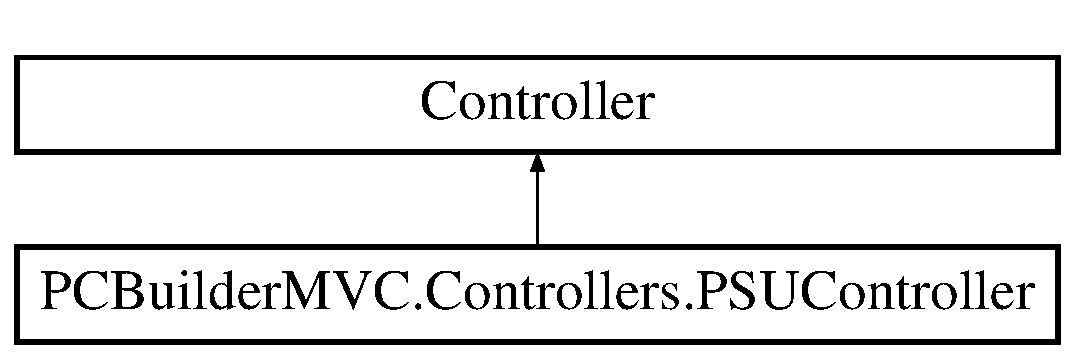
\includegraphics[height=2.000000cm]{class_p_c_builder_m_v_c_1_1_controllers_1_1_p_s_u_controller}
\end{center}
\end{figure}
\subsection*{Public Member Functions}
\begin{DoxyCompactItemize}
\item 
Action\+Result {\bfseries Index} ()\hypertarget{class_p_c_builder_m_v_c_1_1_controllers_1_1_p_s_u_controller_a091077c612db8f41b3fdc91d8f40ee1a}{}\label{class_p_c_builder_m_v_c_1_1_controllers_1_1_p_s_u_controller_a091077c612db8f41b3fdc91d8f40ee1a}

\item 
Action\+Result {\bfseries Details} (int?id)\hypertarget{class_p_c_builder_m_v_c_1_1_controllers_1_1_p_s_u_controller_aa11ba9390a2ade5a7780fde7184ad605}{}\label{class_p_c_builder_m_v_c_1_1_controllers_1_1_p_s_u_controller_aa11ba9390a2ade5a7780fde7184ad605}

\item 
Action\+Result {\bfseries Create} ()\hypertarget{class_p_c_builder_m_v_c_1_1_controllers_1_1_p_s_u_controller_aab12c9297ccd422406759d10486b4089}{}\label{class_p_c_builder_m_v_c_1_1_controllers_1_1_p_s_u_controller_aab12c9297ccd422406759d10486b4089}

\item 
Action\+Result {\bfseries Create} (\mbox{[}Bind(Include=\char`\"{}Psu\+Id,Brand,Model,Wattage,Efficiency,Price\char`\"{})\mbox{]} P\+SU p\+SU)\hypertarget{class_p_c_builder_m_v_c_1_1_controllers_1_1_p_s_u_controller_a3f8a86f6901b123fd7f481a9d69f4e85}{}\label{class_p_c_builder_m_v_c_1_1_controllers_1_1_p_s_u_controller_a3f8a86f6901b123fd7f481a9d69f4e85}

\item 
Action\+Result {\bfseries Edit} (int?id)\hypertarget{class_p_c_builder_m_v_c_1_1_controllers_1_1_p_s_u_controller_a0cd44180c3a4e4571745bcc26f4f125a}{}\label{class_p_c_builder_m_v_c_1_1_controllers_1_1_p_s_u_controller_a0cd44180c3a4e4571745bcc26f4f125a}

\item 
Action\+Result {\bfseries Edit} (\mbox{[}Bind(Include=\char`\"{}Psu\+Id,Brand,Model,Wattage,Efficiency,Price\char`\"{})\mbox{]} P\+SU p\+SU)\hypertarget{class_p_c_builder_m_v_c_1_1_controllers_1_1_p_s_u_controller_ad171810d48df24733a5314645121e61b}{}\label{class_p_c_builder_m_v_c_1_1_controllers_1_1_p_s_u_controller_ad171810d48df24733a5314645121e61b}

\item 
Action\+Result {\bfseries Delete} (int?id)\hypertarget{class_p_c_builder_m_v_c_1_1_controllers_1_1_p_s_u_controller_a50c3976316e118165f74e9f9e89dec75}{}\label{class_p_c_builder_m_v_c_1_1_controllers_1_1_p_s_u_controller_a50c3976316e118165f74e9f9e89dec75}

\item 
Action\+Result {\bfseries Delete\+Confirmed} (int id)\hypertarget{class_p_c_builder_m_v_c_1_1_controllers_1_1_p_s_u_controller_ac313c3b328777eb91f58d7fa8dbb6d16}{}\label{class_p_c_builder_m_v_c_1_1_controllers_1_1_p_s_u_controller_ac313c3b328777eb91f58d7fa8dbb6d16}

\end{DoxyCompactItemize}
\subsection*{Protected Member Functions}
\begin{DoxyCompactItemize}
\item 
override void {\bfseries Dispose} (bool disposing)\hypertarget{class_p_c_builder_m_v_c_1_1_controllers_1_1_p_s_u_controller_a6c6ac75cfb1d74033266cdb58f28053b}{}\label{class_p_c_builder_m_v_c_1_1_controllers_1_1_p_s_u_controller_a6c6ac75cfb1d74033266cdb58f28053b}

\end{DoxyCompactItemize}
\subsection*{Private Attributes}
\begin{DoxyCompactItemize}
\item 
\hyperlink{class_p_c_builder_m_v_c_1_1_models_1_1_p_c_builder_entity_models}{P\+C\+Builder\+Entity\+Models} {\bfseries db} = new \hyperlink{class_p_c_builder_m_v_c_1_1_models_1_1_p_c_builder_entity_models}{P\+C\+Builder\+Entity\+Models}()\hypertarget{class_p_c_builder_m_v_c_1_1_controllers_1_1_p_s_u_controller_aab5ac6d5e0f7842d4b6c6a05e8ffc692}{}\label{class_p_c_builder_m_v_c_1_1_controllers_1_1_p_s_u_controller_aab5ac6d5e0f7842d4b6c6a05e8ffc692}

\end{DoxyCompactItemize}


\subsection{Detailed Description}
P\+SU controller class to handle P\+SU views interaction. 

\begin{DoxySeeAlso}{See also}
System.\+Web.\+Mvc.\+Controller


\end{DoxySeeAlso}


Definition at line 17 of file P\+S\+U\+Controller.\+cs.



The documentation for this class was generated from the following file\+:\begin{DoxyCompactItemize}
\item 
C\+:/\+Users/nh228u08/\+Desktop/\+Final\+Project/\+Final\+Project/\+P\+C\+Builder/\+P\+C\+Builder\+M\+V\+C/\+Controllers/P\+S\+U\+Controller.\+cs\end{DoxyCompactItemize}

\hypertarget{class_p_c_builder_forms_1_1_questionnaire}{}\section{P\+C\+Builder\+Forms.\+Questionnaire Class Reference}
\label{class_p_c_builder_forms_1_1_questionnaire}\index{P\+C\+Builder\+Forms.\+Questionnaire@{P\+C\+Builder\+Forms.\+Questionnaire}}


\hyperlink{class_p_c_builder_forms_1_1_questionnaire}{Questionnaire}  


Inheritance diagram for P\+C\+Builder\+Forms.\+Questionnaire\+:\begin{figure}[H]
\begin{center}
\leavevmode
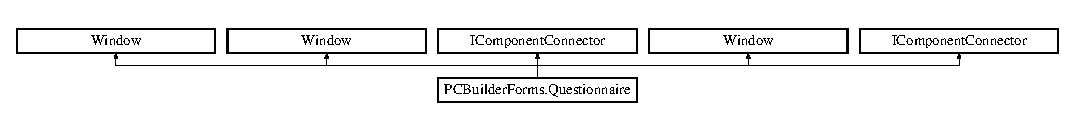
\includegraphics[height=1.148718cm]{class_p_c_builder_forms_1_1_questionnaire}
\end{center}
\end{figure}
\subsection*{Public Member Functions}
\begin{DoxyCompactItemize}
\item 
void \hyperlink{class_p_c_builder_forms_1_1_questionnaire_a89db3c8c78b52416caa22372430d1e6e}{Initialize\+Component} ()
\begin{DoxyCompactList}\small\item\em Initialize\+Component \end{DoxyCompactList}\item 
void \hyperlink{class_p_c_builder_forms_1_1_questionnaire_a89db3c8c78b52416caa22372430d1e6e}{Initialize\+Component} ()
\begin{DoxyCompactList}\small\item\em Initialize\+Component \end{DoxyCompactList}\item 
\hyperlink{class_p_c_builder_forms_1_1_questionnaire_a8adf8b22d2427f03949f3df37f99ce2d}{Questionnaire} ()
\begin{DoxyCompactList}\small\item\em Initializes a new instance of the \hyperlink{class_p_c_builder_forms_1_1_questionnaire}{Questionnaire} class. \end{DoxyCompactList}\end{DoxyCompactItemize}
\subsection*{Package Attributes}
\begin{DoxyCompactItemize}
\item 
System.\+Windows.\+Controls.\+Slider {\bfseries sld\+Performance}\hypertarget{class_p_c_builder_forms_1_1_questionnaire_ac3267ec4c1147b071b1999f5fdd2c9e0}{}\label{class_p_c_builder_forms_1_1_questionnaire_ac3267ec4c1147b071b1999f5fdd2c9e0}

\item 
System.\+Windows.\+Controls.\+Label {\bfseries lbl\+Performance}\hypertarget{class_p_c_builder_forms_1_1_questionnaire_a55404df979e7f8d081d9eb01e0f1f9d2}{}\label{class_p_c_builder_forms_1_1_questionnaire_a55404df979e7f8d081d9eb01e0f1f9d2}

\item 
System.\+Windows.\+Controls.\+Label {\bfseries lbl\+Appx\+Dollars\+Label}\hypertarget{class_p_c_builder_forms_1_1_questionnaire_af6e8662a5f98ec6b0ea9a83c32194c14}{}\label{class_p_c_builder_forms_1_1_questionnaire_af6e8662a5f98ec6b0ea9a83c32194c14}

\item 
System.\+Windows.\+Controls.\+Label {\bfseries lbl\+Appx\+Dollars}\hypertarget{class_p_c_builder_forms_1_1_questionnaire_ab110107164e6fa6bb5066a9019ef3472}{}\label{class_p_c_builder_forms_1_1_questionnaire_ab110107164e6fa6bb5066a9019ef3472}

\item 
System.\+Windows.\+Controls.\+Label {\bfseries lbl\+Use}\hypertarget{class_p_c_builder_forms_1_1_questionnaire_a1fca841040d260bb0c2e38609d80164d}{}\label{class_p_c_builder_forms_1_1_questionnaire_a1fca841040d260bb0c2e38609d80164d}

\item 
System.\+Windows.\+Controls.\+Check\+Box {\bfseries chk\+Use\+Basic}\hypertarget{class_p_c_builder_forms_1_1_questionnaire_abfc851eadf07f61c9baf4b084dba1c6e}{}\label{class_p_c_builder_forms_1_1_questionnaire_abfc851eadf07f61c9baf4b084dba1c6e}

\item 
System.\+Windows.\+Controls.\+Check\+Box {\bfseries chk\+Use\+Video\+Edit}\hypertarget{class_p_c_builder_forms_1_1_questionnaire_a22d8067caf3fddbc5e2ad0c122b65b66}{}\label{class_p_c_builder_forms_1_1_questionnaire_a22d8067caf3fddbc5e2ad0c122b65b66}

\item 
System.\+Windows.\+Controls.\+Check\+Box {\bfseries chk\+Use\+Gaming}\hypertarget{class_p_c_builder_forms_1_1_questionnaire_a01e1cbcd2cade5a159bf07c8a38a1ba1}{}\label{class_p_c_builder_forms_1_1_questionnaire_a01e1cbcd2cade5a159bf07c8a38a1ba1}

\item 
System.\+Windows.\+Controls.\+Check\+Box {\bfseries chk\+Use\+Development}\hypertarget{class_p_c_builder_forms_1_1_questionnaire_aa5e3a716f12c8230813c1ea7e6dbe066}{}\label{class_p_c_builder_forms_1_1_questionnaire_aa5e3a716f12c8230813c1ea7e6dbe066}

\item 
System.\+Windows.\+Controls.\+Check\+Box {\bfseries chk\+Use\+Office\+Moderate}\hypertarget{class_p_c_builder_forms_1_1_questionnaire_ac9b48ad0ed24356de2eca76f241a404a}{}\label{class_p_c_builder_forms_1_1_questionnaire_ac9b48ad0ed24356de2eca76f241a404a}

\item 
System.\+Windows.\+Controls.\+Text\+Block {\bfseries lbl\+Budget\+Notice}\hypertarget{class_p_c_builder_forms_1_1_questionnaire_ad4b2f99b09dba09b72c0a30c5de2889b}{}\label{class_p_c_builder_forms_1_1_questionnaire_ad4b2f99b09dba09b72c0a30c5de2889b}

\item 
System.\+Windows.\+Controls.\+Button {\bfseries btn\+Accept}\hypertarget{class_p_c_builder_forms_1_1_questionnaire_acd21293e6eba54ed7ae80b1961396cb2}{}\label{class_p_c_builder_forms_1_1_questionnaire_acd21293e6eba54ed7ae80b1961396cb2}

\item 
System.\+Windows.\+Controls.\+Button {\bfseries btn\+Reset}\hypertarget{class_p_c_builder_forms_1_1_questionnaire_a98f29008e5166e3805e78b4b3f3cde5a}{}\label{class_p_c_builder_forms_1_1_questionnaire_a98f29008e5166e3805e78b4b3f3cde5a}

\item 
System.\+Windows.\+Controls.\+Button {\bfseries btn\+Cancel}\hypertarget{class_p_c_builder_forms_1_1_questionnaire_aa430b93d2bfaea7fd7ab11efde8fc43b}{}\label{class_p_c_builder_forms_1_1_questionnaire_aa430b93d2bfaea7fd7ab11efde8fc43b}

\item 
System.\+Windows.\+Controls.\+Slider {\bfseries sld\+Storage\+Size}\hypertarget{class_p_c_builder_forms_1_1_questionnaire_a80489b03c4fd52c7068fa7c56dda5534}{}\label{class_p_c_builder_forms_1_1_questionnaire_a80489b03c4fd52c7068fa7c56dda5534}

\item 
System.\+Windows.\+Controls.\+Label {\bfseries lbl\+Storage\+Size\+Label}\hypertarget{class_p_c_builder_forms_1_1_questionnaire_a8b222ca3676f8806e7d4c41165900f87}{}\label{class_p_c_builder_forms_1_1_questionnaire_a8b222ca3676f8806e7d4c41165900f87}

\item 
System.\+Windows.\+Controls.\+Label {\bfseries lbl\+Storage\+Size}\hypertarget{class_p_c_builder_forms_1_1_questionnaire_a64334da3c950cbe2c1d69e132987da9f}{}\label{class_p_c_builder_forms_1_1_questionnaire_a64334da3c950cbe2c1d69e132987da9f}

\item 
System.\+Windows.\+Controls.\+Label {\bfseries lbl\+Storage\+Size\+GB}\hypertarget{class_p_c_builder_forms_1_1_questionnaire_a7b0d0ecbfbc74b6d565a42bb4141fbf4}{}\label{class_p_c_builder_forms_1_1_questionnaire_a7b0d0ecbfbc74b6d565a42bb4141fbf4}

\item 
System.\+Windows.\+Controls.\+Label {\bfseries lbl\+Storage\+Type}\hypertarget{class_p_c_builder_forms_1_1_questionnaire_a7f8e282593378445f3e6454297928f0c}{}\label{class_p_c_builder_forms_1_1_questionnaire_a7f8e282593378445f3e6454297928f0c}

\item 
System.\+Windows.\+Controls.\+Group\+Box {\bfseries grp\+Storage\+Type}\hypertarget{class_p_c_builder_forms_1_1_questionnaire_aacb718674bd68956728ca4e7d4f24f20}{}\label{class_p_c_builder_forms_1_1_questionnaire_aacb718674bd68956728ca4e7d4f24f20}

\item 
System.\+Windows.\+Controls.\+Radio\+Button {\bfseries rad\+S\+SD}\hypertarget{class_p_c_builder_forms_1_1_questionnaire_abaaba55fd7be22a9e7dd881a411ad074}{}\label{class_p_c_builder_forms_1_1_questionnaire_abaaba55fd7be22a9e7dd881a411ad074}

\item 
System.\+Windows.\+Controls.\+Radio\+Button {\bfseries rad\+H\+DD}\hypertarget{class_p_c_builder_forms_1_1_questionnaire_a50611bac3cc1a32bf7cd7cab900d19f4}{}\label{class_p_c_builder_forms_1_1_questionnaire_a50611bac3cc1a32bf7cd7cab900d19f4}

\item 
System.\+Windows.\+Controls.\+Group\+Box {\bfseries grp\+R\+A\+M\+Choices}\hypertarget{class_p_c_builder_forms_1_1_questionnaire_adf88f1d08662bc0b93ba36ae5d6e3cd7}{}\label{class_p_c_builder_forms_1_1_questionnaire_adf88f1d08662bc0b93ba36ae5d6e3cd7}

\item 
System.\+Windows.\+Controls.\+Radio\+Button {\bfseries rad\+R\+A\+M\+Recommended}\hypertarget{class_p_c_builder_forms_1_1_questionnaire_a9667e48b87ba5ca17958376e62f85bfc}{}\label{class_p_c_builder_forms_1_1_questionnaire_a9667e48b87ba5ca17958376e62f85bfc}

\item 
System.\+Windows.\+Controls.\+Radio\+Button {\bfseries rad\+R\+A\+M\+Select\+Manual}\hypertarget{class_p_c_builder_forms_1_1_questionnaire_a7621a4de2b14d731da3e9be5853deedf}{}\label{class_p_c_builder_forms_1_1_questionnaire_a7621a4de2b14d731da3e9be5853deedf}

\item 
System.\+Windows.\+Controls.\+Slider {\bfseries sld\+Ram\+Size}\hypertarget{class_p_c_builder_forms_1_1_questionnaire_a6a563a88382357ef8eee89decdb80e8b}{}\label{class_p_c_builder_forms_1_1_questionnaire_a6a563a88382357ef8eee89decdb80e8b}

\item 
System.\+Windows.\+Controls.\+Label {\bfseries lbl\+Manual\+Ram\+Select}\hypertarget{class_p_c_builder_forms_1_1_questionnaire_a19d7d3f5d3cc2141b9d0798cfe8a9852}{}\label{class_p_c_builder_forms_1_1_questionnaire_a19d7d3f5d3cc2141b9d0798cfe8a9852}

\item 
System.\+Windows.\+Controls.\+Label {\bfseries lbl\+Manual\+Ram\+Select\+Label}\hypertarget{class_p_c_builder_forms_1_1_questionnaire_a5f67de61e73e2579def21ff5bc7ab378}{}\label{class_p_c_builder_forms_1_1_questionnaire_a5f67de61e73e2579def21ff5bc7ab378}

\item 
System.\+Windows.\+Controls.\+Slider {\bfseries sld\+Num\+Cores}\hypertarget{class_p_c_builder_forms_1_1_questionnaire_a7714f0334ab693222eceb856e53aedef}{}\label{class_p_c_builder_forms_1_1_questionnaire_a7714f0334ab693222eceb856e53aedef}

\item 
System.\+Windows.\+Controls.\+Label {\bfseries lbl\+Num\+Cores\+Label}\hypertarget{class_p_c_builder_forms_1_1_questionnaire_ae0a847f6e0a937fe43e28d65b82949ab}{}\label{class_p_c_builder_forms_1_1_questionnaire_ae0a847f6e0a937fe43e28d65b82949ab}

\item 
System.\+Windows.\+Controls.\+Label {\bfseries lbl\+Num\+Cores}\hypertarget{class_p_c_builder_forms_1_1_questionnaire_ae095cf3231846bbb3c840772a127508e}{}\label{class_p_c_builder_forms_1_1_questionnaire_ae095cf3231846bbb3c840772a127508e}

\item 
System.\+Windows.\+Controls.\+Group\+Box {\bfseries grp\+Case\+Size}\hypertarget{class_p_c_builder_forms_1_1_questionnaire_a265f59b48d91297e31afc2bf6f6cc71f}{}\label{class_p_c_builder_forms_1_1_questionnaire_a265f59b48d91297e31afc2bf6f6cc71f}

\item 
System.\+Windows.\+Controls.\+Radio\+Button {\bfseries rad\+Case\+Size\+Full}\hypertarget{class_p_c_builder_forms_1_1_questionnaire_a089c98cd9645269b160e120802ee6291}{}\label{class_p_c_builder_forms_1_1_questionnaire_a089c98cd9645269b160e120802ee6291}

\item 
System.\+Windows.\+Controls.\+Radio\+Button {\bfseries rad\+Case\+Size\+Mid}\hypertarget{class_p_c_builder_forms_1_1_questionnaire_a9da362816e5a9028ac621eadfa920084}{}\label{class_p_c_builder_forms_1_1_questionnaire_a9da362816e5a9028ac621eadfa920084}

\item 
System.\+Windows.\+Controls.\+Radio\+Button {\bfseries rad\+Case\+Size\+Micro}\hypertarget{class_p_c_builder_forms_1_1_questionnaire_af2a207060c7db62e28a4e51069ebbfb2}{}\label{class_p_c_builder_forms_1_1_questionnaire_af2a207060c7db62e28a4e51069ebbfb2}

\item 
System.\+Windows.\+Controls.\+Radio\+Button {\bfseries rad\+Case\+Size\+Mini}\hypertarget{class_p_c_builder_forms_1_1_questionnaire_a171661dc73623f275c82089ac80e92b8}{}\label{class_p_c_builder_forms_1_1_questionnaire_a171661dc73623f275c82089ac80e92b8}

\item 
System.\+Windows.\+Controls.\+Radio\+Button {\bfseries rad\+Case\+Size\+Console}\hypertarget{class_p_c_builder_forms_1_1_questionnaire_a5122088ec1da5fdfeff7f73e7a1ed7d8}{}\label{class_p_c_builder_forms_1_1_questionnaire_a5122088ec1da5fdfeff7f73e7a1ed7d8}

\item 
System.\+Windows.\+Controls.\+Group\+Box {\bfseries grp\+Optical}\hypertarget{class_p_c_builder_forms_1_1_questionnaire_a7a94ab8ff1888935eb071e4c25efb276}{}\label{class_p_c_builder_forms_1_1_questionnaire_a7a94ab8ff1888935eb071e4c25efb276}

\item 
System.\+Windows.\+Controls.\+Radio\+Button {\bfseries rad\+B\+R\+Burner}\hypertarget{class_p_c_builder_forms_1_1_questionnaire_a439d90d008d5082cea79a9223280613e}{}\label{class_p_c_builder_forms_1_1_questionnaire_a439d90d008d5082cea79a9223280613e}

\item 
System.\+Windows.\+Controls.\+Radio\+Button {\bfseries rad\+B\+R\+Reader}\hypertarget{class_p_c_builder_forms_1_1_questionnaire_a1737317fe4bb2105fc33d6a85eb3bd80}{}\label{class_p_c_builder_forms_1_1_questionnaire_a1737317fe4bb2105fc33d6a85eb3bd80}

\item 
System.\+Windows.\+Controls.\+Radio\+Button {\bfseries rad\+D\+V\+D\+Burner}\hypertarget{class_p_c_builder_forms_1_1_questionnaire_a4dbb291702e5c164203150799da2d179}{}\label{class_p_c_builder_forms_1_1_questionnaire_a4dbb291702e5c164203150799da2d179}

\item 
System.\+Windows.\+Controls.\+Radio\+Button {\bfseries rad\+Optical\+None}\hypertarget{class_p_c_builder_forms_1_1_questionnaire_a042a2900dee726caecea62754540e6a6}{}\label{class_p_c_builder_forms_1_1_questionnaire_a042a2900dee726caecea62754540e6a6}

\end{DoxyCompactItemize}
\subsection*{Properties}
\begin{DoxyCompactItemize}
\item 
\hyperlink{class_business_objects_1_1_finalized_build}{Finalized\+Build} {\bfseries FB}\hspace{0.3cm}{\ttfamily  \mbox{[}get, set\mbox{]}}\hypertarget{class_p_c_builder_forms_1_1_questionnaire_afa53e86f988e8542c4355b18b4d61382}{}\label{class_p_c_builder_forms_1_1_questionnaire_afa53e86f988e8542c4355b18b4d61382}

\item 
\hyperlink{class_business_objects_1_1_questionnaire_results}{Questionnaire\+Results} {\bfseries QR}\hspace{0.3cm}{\ttfamily  \mbox{[}get, set\mbox{]}}\hypertarget{class_p_c_builder_forms_1_1_questionnaire_ac4a23f37f67fd6346138c0a480434dad}{}\label{class_p_c_builder_forms_1_1_questionnaire_ac4a23f37f67fd6346138c0a480434dad}

\end{DoxyCompactItemize}
\subsection*{Private Member Functions}
\begin{DoxyCompactItemize}
\item 
void System.\+Windows.\+Markup.\+I\+Component\+Connector. {\bfseries Connect} (int connection\+Id, object target)\hypertarget{class_p_c_builder_forms_1_1_questionnaire_af04ecdbdb6d1206ff7b04627ea55c08e}{}\label{class_p_c_builder_forms_1_1_questionnaire_af04ecdbdb6d1206ff7b04627ea55c08e}

\item 
void System.\+Windows.\+Markup.\+I\+Component\+Connector. {\bfseries Connect} (int connection\+Id, object target)\hypertarget{class_p_c_builder_forms_1_1_questionnaire_af04ecdbdb6d1206ff7b04627ea55c08e}{}\label{class_p_c_builder_forms_1_1_questionnaire_af04ecdbdb6d1206ff7b04627ea55c08e}

\item 
void \hyperlink{class_p_c_builder_forms_1_1_questionnaire_a4c5659e3c84f9eb08287fa86ad3a4684}{sld\+Performance\+\_\+\+Value\+Changed} (object sender, Routed\+Property\+Changed\+Event\+Args$<$ double $>$ e)
\begin{DoxyCompactList}\small\item\em Handles the Value\+Changed event of the sld\+Performance control. \end{DoxyCompactList}\item 
void \hyperlink{class_p_c_builder_forms_1_1_questionnaire_abd5934363e01fc284501e7dca14cf0e1}{rad\+R\+A\+M\+Select\+Manual\+\_\+\+Checked} (object sender, Routed\+Event\+Args e)
\begin{DoxyCompactList}\small\item\em Handles the Checked event of the rad\+R\+A\+M\+Select\+Manual control. \end{DoxyCompactList}\item 
void \hyperlink{class_p_c_builder_forms_1_1_questionnaire_aafa36d5d99af61aec682aadc59f6b6b7}{rad\+R\+A\+M\+Select\+Manual\+\_\+\+Unchecked} (object sender, Routed\+Event\+Args e)
\begin{DoxyCompactList}\small\item\em Handles the Unchecked event of the rad\+R\+A\+M\+Select\+Manual control. \end{DoxyCompactList}\item 
void \hyperlink{class_p_c_builder_forms_1_1_questionnaire_a95e76d557be209143133d97d71e40bdd}{btn\+Reset\+\_\+\+Click} (object sender, Routed\+Event\+Args e)
\begin{DoxyCompactList}\small\item\em Handles the Click event of the btn\+Reset control. \end{DoxyCompactList}\item 
void \hyperlink{class_p_c_builder_forms_1_1_questionnaire_a21b5d339c61d10bdc83bdac62cebccd6}{btn\+Cancel\+\_\+\+Click} (object sender, Routed\+Event\+Args e)
\begin{DoxyCompactList}\small\item\em Handles the Click event of the btn\+Cancel control. \end{DoxyCompactList}\item 
void \hyperlink{class_p_c_builder_forms_1_1_questionnaire_a57d92628463485e31d68831240f1a97d}{Reset\+Form} ()
\begin{DoxyCompactList}\small\item\em Resets the form. \end{DoxyCompactList}\item 
void \hyperlink{class_p_c_builder_forms_1_1_questionnaire_a2000ae75279c69732241fe71e4b66b89}{btn\+Accept\+\_\+\+Click} (object sender, Routed\+Event\+Args e)
\begin{DoxyCompactList}\small\item\em Handles the Click event of the btn\+Accept control. \end{DoxyCompactList}\end{DoxyCompactItemize}
\subsection*{Private Attributes}
\begin{DoxyCompactItemize}
\item 
bool {\bfseries \+\_\+content\+Loaded}\hypertarget{class_p_c_builder_forms_1_1_questionnaire_ab9d56bf1f26e74f376becccf304a8f54}{}\label{class_p_c_builder_forms_1_1_questionnaire_ab9d56bf1f26e74f376becccf304a8f54}

\end{DoxyCompactItemize}


\subsection{Detailed Description}
\hyperlink{class_p_c_builder_forms_1_1_questionnaire}{Questionnaire} 

Interaction logic for Questionnaire.\+xaml 

Definition at line 41 of file Questionnaire.\+g.\+cs.



\subsection{Constructor \& Destructor Documentation}
\index{P\+C\+Builder\+Forms\+::\+Questionnaire@{P\+C\+Builder\+Forms\+::\+Questionnaire}!Questionnaire@{Questionnaire}}
\index{Questionnaire@{Questionnaire}!P\+C\+Builder\+Forms\+::\+Questionnaire@{P\+C\+Builder\+Forms\+::\+Questionnaire}}
\subsubsection[{\texorpdfstring{Questionnaire()}{Questionnaire()}}]{\setlength{\rightskip}{0pt plus 5cm}P\+C\+Builder\+Forms.\+Questionnaire.\+Questionnaire (
\begin{DoxyParamCaption}
{}
\end{DoxyParamCaption}
)}\hypertarget{class_p_c_builder_forms_1_1_questionnaire_a8adf8b22d2427f03949f3df37f99ce2d}{}\label{class_p_c_builder_forms_1_1_questionnaire_a8adf8b22d2427f03949f3df37f99ce2d}


Initializes a new instance of the \hyperlink{class_p_c_builder_forms_1_1_questionnaire}{Questionnaire} class. 



Definition at line 32 of file Questionnaire.\+xaml.\+cs.



\subsection{Member Function Documentation}
\index{P\+C\+Builder\+Forms\+::\+Questionnaire@{P\+C\+Builder\+Forms\+::\+Questionnaire}!btn\+Accept\+\_\+\+Click@{btn\+Accept\+\_\+\+Click}}
\index{btn\+Accept\+\_\+\+Click@{btn\+Accept\+\_\+\+Click}!P\+C\+Builder\+Forms\+::\+Questionnaire@{P\+C\+Builder\+Forms\+::\+Questionnaire}}
\subsubsection[{\texorpdfstring{btn\+Accept\+\_\+\+Click(object sender, Routed\+Event\+Args e)}{btnAccept_Click(object sender, RoutedEventArgs e)}}]{\setlength{\rightskip}{0pt plus 5cm}void P\+C\+Builder\+Forms.\+Questionnaire.\+btn\+Accept\+\_\+\+Click (
\begin{DoxyParamCaption}
\item[{object}]{sender, }
\item[{Routed\+Event\+Args}]{e}
\end{DoxyParamCaption}
)\hspace{0.3cm}{\ttfamily [private]}}\hypertarget{class_p_c_builder_forms_1_1_questionnaire_a2000ae75279c69732241fe71e4b66b89}{}\label{class_p_c_builder_forms_1_1_questionnaire_a2000ae75279c69732241fe71e4b66b89}


Handles the Click event of the btn\+Accept control. 


\begin{DoxyParams}{Parameters}
{\em sender} & The source of the event.\\
\hline
{\em e} & The Routed\+Event\+Args instance containing the event data.\\
\hline
\end{DoxyParams}


Definition at line 123 of file Questionnaire.\+xaml.\+cs.

\index{P\+C\+Builder\+Forms\+::\+Questionnaire@{P\+C\+Builder\+Forms\+::\+Questionnaire}!btn\+Cancel\+\_\+\+Click@{btn\+Cancel\+\_\+\+Click}}
\index{btn\+Cancel\+\_\+\+Click@{btn\+Cancel\+\_\+\+Click}!P\+C\+Builder\+Forms\+::\+Questionnaire@{P\+C\+Builder\+Forms\+::\+Questionnaire}}
\subsubsection[{\texorpdfstring{btn\+Cancel\+\_\+\+Click(object sender, Routed\+Event\+Args e)}{btnCancel_Click(object sender, RoutedEventArgs e)}}]{\setlength{\rightskip}{0pt plus 5cm}void P\+C\+Builder\+Forms.\+Questionnaire.\+btn\+Cancel\+\_\+\+Click (
\begin{DoxyParamCaption}
\item[{object}]{sender, }
\item[{Routed\+Event\+Args}]{e}
\end{DoxyParamCaption}
)\hspace{0.3cm}{\ttfamily [private]}}\hypertarget{class_p_c_builder_forms_1_1_questionnaire_a21b5d339c61d10bdc83bdac62cebccd6}{}\label{class_p_c_builder_forms_1_1_questionnaire_a21b5d339c61d10bdc83bdac62cebccd6}


Handles the Click event of the btn\+Cancel control. 


\begin{DoxyParams}{Parameters}
{\em sender} & The source of the event.\\
\hline
{\em e} & The Routed\+Event\+Args instance containing the event data.\\
\hline
\end{DoxyParams}


Definition at line 89 of file Questionnaire.\+xaml.\+cs.

\index{P\+C\+Builder\+Forms\+::\+Questionnaire@{P\+C\+Builder\+Forms\+::\+Questionnaire}!btn\+Reset\+\_\+\+Click@{btn\+Reset\+\_\+\+Click}}
\index{btn\+Reset\+\_\+\+Click@{btn\+Reset\+\_\+\+Click}!P\+C\+Builder\+Forms\+::\+Questionnaire@{P\+C\+Builder\+Forms\+::\+Questionnaire}}
\subsubsection[{\texorpdfstring{btn\+Reset\+\_\+\+Click(object sender, Routed\+Event\+Args e)}{btnReset_Click(object sender, RoutedEventArgs e)}}]{\setlength{\rightskip}{0pt plus 5cm}void P\+C\+Builder\+Forms.\+Questionnaire.\+btn\+Reset\+\_\+\+Click (
\begin{DoxyParamCaption}
\item[{object}]{sender, }
\item[{Routed\+Event\+Args}]{e}
\end{DoxyParamCaption}
)\hspace{0.3cm}{\ttfamily [private]}}\hypertarget{class_p_c_builder_forms_1_1_questionnaire_a95e76d557be209143133d97d71e40bdd}{}\label{class_p_c_builder_forms_1_1_questionnaire_a95e76d557be209143133d97d71e40bdd}


Handles the Click event of the btn\+Reset control. 


\begin{DoxyParams}{Parameters}
{\em sender} & The source of the event.\\
\hline
{\em e} & The Routed\+Event\+Args instance containing the event data.\\
\hline
\end{DoxyParams}


Definition at line 75 of file Questionnaire.\+xaml.\+cs.

\index{P\+C\+Builder\+Forms\+::\+Questionnaire@{P\+C\+Builder\+Forms\+::\+Questionnaire}!Initialize\+Component@{Initialize\+Component}}
\index{Initialize\+Component@{Initialize\+Component}!P\+C\+Builder\+Forms\+::\+Questionnaire@{P\+C\+Builder\+Forms\+::\+Questionnaire}}
\subsubsection[{\texorpdfstring{Initialize\+Component()}{InitializeComponent()}}]{\setlength{\rightskip}{0pt plus 5cm}void P\+C\+Builder\+Forms.\+Questionnaire.\+Initialize\+Component (
\begin{DoxyParamCaption}
{}
\end{DoxyParamCaption}
)}\hypertarget{class_p_c_builder_forms_1_1_questionnaire_a89db3c8c78b52416caa22372430d1e6e}{}\label{class_p_c_builder_forms_1_1_questionnaire_a89db3c8c78b52416caa22372430d1e6e}


Initialize\+Component 



Definition at line 386 of file Questionnaire.\+g.\+cs.

\index{P\+C\+Builder\+Forms\+::\+Questionnaire@{P\+C\+Builder\+Forms\+::\+Questionnaire}!Initialize\+Component@{Initialize\+Component}}
\index{Initialize\+Component@{Initialize\+Component}!P\+C\+Builder\+Forms\+::\+Questionnaire@{P\+C\+Builder\+Forms\+::\+Questionnaire}}
\subsubsection[{\texorpdfstring{Initialize\+Component()}{InitializeComponent()}}]{\setlength{\rightskip}{0pt plus 5cm}void P\+C\+Builder\+Forms.\+Questionnaire.\+Initialize\+Component (
\begin{DoxyParamCaption}
{}
\end{DoxyParamCaption}
)}\hypertarget{class_p_c_builder_forms_1_1_questionnaire_a89db3c8c78b52416caa22372430d1e6e}{}\label{class_p_c_builder_forms_1_1_questionnaire_a89db3c8c78b52416caa22372430d1e6e}


Initialize\+Component 



Definition at line 386 of file Questionnaire.\+g.\+i.\+cs.

\index{P\+C\+Builder\+Forms\+::\+Questionnaire@{P\+C\+Builder\+Forms\+::\+Questionnaire}!rad\+R\+A\+M\+Select\+Manual\+\_\+\+Checked@{rad\+R\+A\+M\+Select\+Manual\+\_\+\+Checked}}
\index{rad\+R\+A\+M\+Select\+Manual\+\_\+\+Checked@{rad\+R\+A\+M\+Select\+Manual\+\_\+\+Checked}!P\+C\+Builder\+Forms\+::\+Questionnaire@{P\+C\+Builder\+Forms\+::\+Questionnaire}}
\subsubsection[{\texorpdfstring{rad\+R\+A\+M\+Select\+Manual\+\_\+\+Checked(object sender, Routed\+Event\+Args e)}{radRAMSelectManual_Checked(object sender, RoutedEventArgs e)}}]{\setlength{\rightskip}{0pt plus 5cm}void P\+C\+Builder\+Forms.\+Questionnaire.\+rad\+R\+A\+M\+Select\+Manual\+\_\+\+Checked (
\begin{DoxyParamCaption}
\item[{object}]{sender, }
\item[{Routed\+Event\+Args}]{e}
\end{DoxyParamCaption}
)\hspace{0.3cm}{\ttfamily [private]}}\hypertarget{class_p_c_builder_forms_1_1_questionnaire_abd5934363e01fc284501e7dca14cf0e1}{}\label{class_p_c_builder_forms_1_1_questionnaire_abd5934363e01fc284501e7dca14cf0e1}


Handles the Checked event of the rad\+R\+A\+M\+Select\+Manual control. 


\begin{DoxyParams}{Parameters}
{\em sender} & The source of the event.\\
\hline
{\em e} & The Routed\+Event\+Args instance containing the event data.\\
\hline
\end{DoxyParams}


Definition at line 51 of file Questionnaire.\+xaml.\+cs.

\index{P\+C\+Builder\+Forms\+::\+Questionnaire@{P\+C\+Builder\+Forms\+::\+Questionnaire}!rad\+R\+A\+M\+Select\+Manual\+\_\+\+Unchecked@{rad\+R\+A\+M\+Select\+Manual\+\_\+\+Unchecked}}
\index{rad\+R\+A\+M\+Select\+Manual\+\_\+\+Unchecked@{rad\+R\+A\+M\+Select\+Manual\+\_\+\+Unchecked}!P\+C\+Builder\+Forms\+::\+Questionnaire@{P\+C\+Builder\+Forms\+::\+Questionnaire}}
\subsubsection[{\texorpdfstring{rad\+R\+A\+M\+Select\+Manual\+\_\+\+Unchecked(object sender, Routed\+Event\+Args e)}{radRAMSelectManual_Unchecked(object sender, RoutedEventArgs e)}}]{\setlength{\rightskip}{0pt plus 5cm}void P\+C\+Builder\+Forms.\+Questionnaire.\+rad\+R\+A\+M\+Select\+Manual\+\_\+\+Unchecked (
\begin{DoxyParamCaption}
\item[{object}]{sender, }
\item[{Routed\+Event\+Args}]{e}
\end{DoxyParamCaption}
)\hspace{0.3cm}{\ttfamily [private]}}\hypertarget{class_p_c_builder_forms_1_1_questionnaire_aafa36d5d99af61aec682aadc59f6b6b7}{}\label{class_p_c_builder_forms_1_1_questionnaire_aafa36d5d99af61aec682aadc59f6b6b7}


Handles the Unchecked event of the rad\+R\+A\+M\+Select\+Manual control. 


\begin{DoxyParams}{Parameters}
{\em sender} & The source of the event.\\
\hline
{\em e} & The Routed\+Event\+Args instance containing the event data.\\
\hline
\end{DoxyParams}


Definition at line 63 of file Questionnaire.\+xaml.\+cs.

\index{P\+C\+Builder\+Forms\+::\+Questionnaire@{P\+C\+Builder\+Forms\+::\+Questionnaire}!Reset\+Form@{Reset\+Form}}
\index{Reset\+Form@{Reset\+Form}!P\+C\+Builder\+Forms\+::\+Questionnaire@{P\+C\+Builder\+Forms\+::\+Questionnaire}}
\subsubsection[{\texorpdfstring{Reset\+Form()}{ResetForm()}}]{\setlength{\rightskip}{0pt plus 5cm}void P\+C\+Builder\+Forms.\+Questionnaire.\+Reset\+Form (
\begin{DoxyParamCaption}
{}
\end{DoxyParamCaption}
)\hspace{0.3cm}{\ttfamily [private]}}\hypertarget{class_p_c_builder_forms_1_1_questionnaire_a57d92628463485e31d68831240f1a97d}{}\label{class_p_c_builder_forms_1_1_questionnaire_a57d92628463485e31d68831240f1a97d}


Resets the form. 



Definition at line 103 of file Questionnaire.\+xaml.\+cs.

\index{P\+C\+Builder\+Forms\+::\+Questionnaire@{P\+C\+Builder\+Forms\+::\+Questionnaire}!sld\+Performance\+\_\+\+Value\+Changed@{sld\+Performance\+\_\+\+Value\+Changed}}
\index{sld\+Performance\+\_\+\+Value\+Changed@{sld\+Performance\+\_\+\+Value\+Changed}!P\+C\+Builder\+Forms\+::\+Questionnaire@{P\+C\+Builder\+Forms\+::\+Questionnaire}}
\subsubsection[{\texorpdfstring{sld\+Performance\+\_\+\+Value\+Changed(object sender, Routed\+Property\+Changed\+Event\+Args$<$ double $>$ e)}{sldPerformance_ValueChanged(object sender, RoutedPropertyChangedEventArgs< double > e)}}]{\setlength{\rightskip}{0pt plus 5cm}void P\+C\+Builder\+Forms.\+Questionnaire.\+sld\+Performance\+\_\+\+Value\+Changed (
\begin{DoxyParamCaption}
\item[{object}]{sender, }
\item[{Routed\+Property\+Changed\+Event\+Args$<$ double $>$}]{e}
\end{DoxyParamCaption}
)\hspace{0.3cm}{\ttfamily [private]}}\hypertarget{class_p_c_builder_forms_1_1_questionnaire_a4c5659e3c84f9eb08287fa86ad3a4684}{}\label{class_p_c_builder_forms_1_1_questionnaire_a4c5659e3c84f9eb08287fa86ad3a4684}


Handles the Value\+Changed event of the sld\+Performance control. 


\begin{DoxyParams}{Parameters}
{\em sender} & The source of the event.\\
\hline
{\em e} & The Routed\+Property\+Changed\+Event\+Args$<$\+System.\+Double$>$ instance containing the event data.\\
\hline
\end{DoxyParams}


Definition at line 42 of file Questionnaire.\+xaml.\+cs.



The documentation for this class was generated from the following files\+:\begin{DoxyCompactItemize}
\item 
C\+:/\+Users/nh228u08/\+Desktop/\+Final\+Project/\+Final\+Project/\+P\+C\+Builder/\+P\+C\+Builder\+Forms/obj/\+Debug/Questionnaire.\+g.\+cs\item 
C\+:/\+Users/nh228u08/\+Desktop/\+Final\+Project/\+Final\+Project/\+P\+C\+Builder/\+P\+C\+Builder\+Forms/obj/\+Debug/Questionnaire.\+g.\+i.\+cs\item 
C\+:/\+Users/nh228u08/\+Desktop/\+Final\+Project/\+Final\+Project/\+P\+C\+Builder/\+P\+C\+Builder\+Forms/Questionnaire.\+xaml.\+cs\end{DoxyCompactItemize}

\hypertarget{class_p_c_builder_m_v_c_1_1_controllers_1_1_questionnaire_controller}{}\section{P\+C\+Builder\+M\+V\+C.\+Controllers.\+Questionnaire\+Controller Class Reference}
\label{class_p_c_builder_m_v_c_1_1_controllers_1_1_questionnaire_controller}\index{P\+C\+Builder\+M\+V\+C.\+Controllers.\+Questionnaire\+Controller@{P\+C\+Builder\+M\+V\+C.\+Controllers.\+Questionnaire\+Controller}}


Questionnaire controller class to handle Questionnaire views interaction.  


Inheritance diagram for P\+C\+Builder\+M\+V\+C.\+Controllers.\+Questionnaire\+Controller\+:\begin{figure}[H]
\begin{center}
\leavevmode
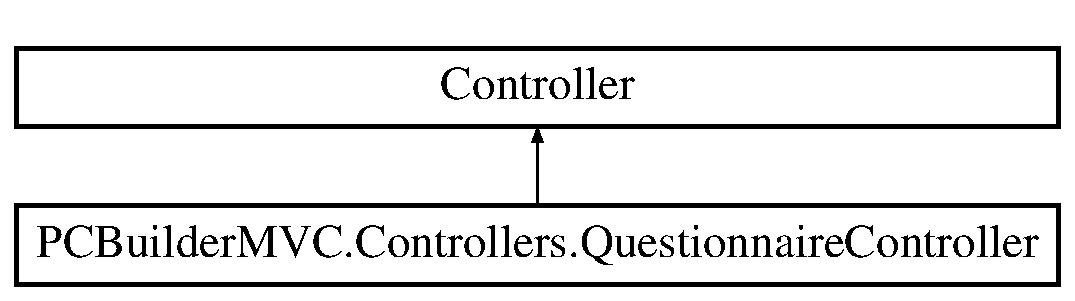
\includegraphics[height=2.000000cm]{class_p_c_builder_m_v_c_1_1_controllers_1_1_questionnaire_controller}
\end{center}
\end{figure}
\subsection*{Public Member Functions}
\begin{DoxyCompactItemize}
\item 
Action\+Result {\bfseries Index} ()\hypertarget{class_p_c_builder_m_v_c_1_1_controllers_1_1_questionnaire_controller_ac7fd83d5be85d3faa104f769f459741e}{}\label{class_p_c_builder_m_v_c_1_1_controllers_1_1_questionnaire_controller_ac7fd83d5be85d3faa104f769f459741e}

\item 
Action\+Result {\bfseries Create} ()\hypertarget{class_p_c_builder_m_v_c_1_1_controllers_1_1_questionnaire_controller_aee74d3623a8572991d23e6718ea5cc23}{}\label{class_p_c_builder_m_v_c_1_1_controllers_1_1_questionnaire_controller_aee74d3623a8572991d23e6718ea5cc23}

\item 
Action\+Result {\bfseries Create} (\mbox{[}Bind(Include=\char`\"{}Questionnaire\+ID,Sld\+Performance,Chk\+Use\+Basic,Chk\+Use\+Video\+Edit,Chk\+Use\+Gaming,Chk\+Use\+Development,Chk\+Use\+Office\+Moderate,Rad\+Resolution720,Rad\+Resolution1080,Rad\+Resolution4k,Sld\+Num\+Monitors,Sld\+Storage\+Size,Rad\+S\+SD,Rad\+H\+DD,Rad\+R\+A\+M\+Recommended,Rad\+R\+A\+M\+Select\+Manual,Sld\+Ram\+Size,Sld\+Num\+Cores,Rad\+Case\+Size\+Full,Rad\+Case\+Size\+Mid,Rad\+Case\+Size\+Micro,Rad\+Case\+Size\+Mini,Rad\+Case\+Size\+Console,Rad\+B\+R\+Burner,Rad\+B\+R\+Reader,Rad\+D\+V\+D\+Burner,Rad\+Optical\+None\char`\"{})\mbox{]} Questionnaire\+View\+Model questionnaire\+View\+Model)\hypertarget{class_p_c_builder_m_v_c_1_1_controllers_1_1_questionnaire_controller_a56e22d7a06a6dd75dca2244a994454da}{}\label{class_p_c_builder_m_v_c_1_1_controllers_1_1_questionnaire_controller_a56e22d7a06a6dd75dca2244a994454da}

\end{DoxyCompactItemize}
\subsection*{Protected Member Functions}
\begin{DoxyCompactItemize}
\item 
override void {\bfseries Dispose} (bool disposing)\hypertarget{class_p_c_builder_m_v_c_1_1_controllers_1_1_questionnaire_controller_a8b20695629cea08ed178104f70efe939}{}\label{class_p_c_builder_m_v_c_1_1_controllers_1_1_questionnaire_controller_a8b20695629cea08ed178104f70efe939}

\end{DoxyCompactItemize}
\subsection*{Private Attributes}
\begin{DoxyCompactItemize}
\item 
\hyperlink{class_p_c_builder_m_v_c_1_1_models_1_1_p_c_builder_entity_models}{P\+C\+Builder\+Entity\+Models} {\bfseries db} = new \hyperlink{class_p_c_builder_m_v_c_1_1_models_1_1_p_c_builder_entity_models}{P\+C\+Builder\+Entity\+Models}()\hypertarget{class_p_c_builder_m_v_c_1_1_controllers_1_1_questionnaire_controller_a664b66f071710f84457bd129929b6777}{}\label{class_p_c_builder_m_v_c_1_1_controllers_1_1_questionnaire_controller_a664b66f071710f84457bd129929b6777}

\end{DoxyCompactItemize}


\subsection{Detailed Description}
Questionnaire controller class to handle Questionnaire views interaction. 

\begin{DoxySeeAlso}{See also}
System.\+Web.\+Mvc.\+Controller


\end{DoxySeeAlso}


Definition at line 19 of file Questionnaire\+Controller.\+cs.



The documentation for this class was generated from the following file\+:\begin{DoxyCompactItemize}
\item 
C\+:/\+Users/nh228u08/\+Desktop/\+Final\+Project/\+Final\+Project/\+P\+C\+Builder/\+P\+C\+Builder\+M\+V\+C/\+Controllers/Questionnaire\+Controller.\+cs\end{DoxyCompactItemize}

\hypertarget{class_business_objects_1_1_questionnaire_results}{}\section{Business\+Objects.\+Questionnaire\+Results Class Reference}
\label{class_business_objects_1_1_questionnaire_results}\index{Business\+Objects.\+Questionnaire\+Results@{Business\+Objects.\+Questionnaire\+Results}}


\hyperlink{class_business_objects_1_1_questionnaire_results}{Questionnaire\+Results} object to hold necessary data on the questionnaire form after submission.  


\subsection*{Public Member Functions}
\begin{DoxyCompactItemize}
\item 
\hyperlink{class_business_objects_1_1_questionnaire_results_af03bf5cea4bc3c29bb2a4b111b6e6a2c}{Questionnaire\+Results} ()
\begin{DoxyCompactList}\small\item\em Initializes a new instance of the \hyperlink{class_business_objects_1_1_questionnaire_results}{Questionnaire\+Results} class. \end{DoxyCompactList}\item 
\hyperlink{class_business_objects_1_1_questionnaire_results_a4e99b6de8ad5c240763baa74ebae2ca4}{Questionnaire\+Results} (double sld\+Performance, bool chk\+Use\+Basic, bool chk\+Use\+Development, bool chk\+Use\+Gaming, bool chk\+Use\+Office\+Moderate, bool chk\+Use\+Video\+Edit, bool rad\+Resolution720, bool rad\+Resolution1080, bool rad\+Resolution4k, double sld\+Num\+Monitors, double sld\+Storage\+Size, bool rad\+S\+SD, bool rad\+H\+DD, bool rad\+R\+A\+M\+Recommended, bool rad\+R\+A\+M\+Select\+Manual, double sld\+Ram\+Size, double sld\+Num\+Cores, bool rad\+Case\+Size\+Full, bool rad\+Case\+Size\+Mid, bool rad\+Case\+Size\+Micro, bool rad\+Case\+Size\+Mini, bool rad\+Case\+Size\+Console, bool rad\+B\+R\+Burner, bool rad\+B\+R\+Reader, bool rad\+D\+V\+D\+Burner, bool rad\+Optical\+None)
\begin{DoxyCompactList}\small\item\em Initializes a new instance of the \hyperlink{class_business_objects_1_1_questionnaire_results}{Questionnaire\+Results} class. \end{DoxyCompactList}\end{DoxyCompactItemize}
\subsection*{Properties}
\begin{DoxyCompactItemize}
\item 
double {\bfseries Sld\+Performance}\hspace{0.3cm}{\ttfamily  \mbox{[}get, set\mbox{]}}\hypertarget{class_business_objects_1_1_questionnaire_results_a6688ec1ee3a89d76362da1d7e33dc636}{}\label{class_business_objects_1_1_questionnaire_results_a6688ec1ee3a89d76362da1d7e33dc636}

\item 
bool {\bfseries Chk\+Use\+Basic}\hspace{0.3cm}{\ttfamily  \mbox{[}get, set\mbox{]}}\hypertarget{class_business_objects_1_1_questionnaire_results_a50640a66fd5f77082f79e232802a1ae3}{}\label{class_business_objects_1_1_questionnaire_results_a50640a66fd5f77082f79e232802a1ae3}

\item 
bool {\bfseries Chk\+Use\+Video\+Edit}\hspace{0.3cm}{\ttfamily  \mbox{[}get, set\mbox{]}}\hypertarget{class_business_objects_1_1_questionnaire_results_a3472f3dc9e3ec8945b73689117b858a2}{}\label{class_business_objects_1_1_questionnaire_results_a3472f3dc9e3ec8945b73689117b858a2}

\item 
bool {\bfseries Chk\+Use\+Gaming}\hspace{0.3cm}{\ttfamily  \mbox{[}get, set\mbox{]}}\hypertarget{class_business_objects_1_1_questionnaire_results_a9360e56e1763fbada54d68f242f30f4c}{}\label{class_business_objects_1_1_questionnaire_results_a9360e56e1763fbada54d68f242f30f4c}

\item 
bool {\bfseries Chk\+Use\+Development}\hspace{0.3cm}{\ttfamily  \mbox{[}get, set\mbox{]}}\hypertarget{class_business_objects_1_1_questionnaire_results_a71afc6ff6bcbdb3b9d76d619ed9541fa}{}\label{class_business_objects_1_1_questionnaire_results_a71afc6ff6bcbdb3b9d76d619ed9541fa}

\item 
bool {\bfseries Chk\+Use\+Office\+Moderate}\hspace{0.3cm}{\ttfamily  \mbox{[}get, set\mbox{]}}\hypertarget{class_business_objects_1_1_questionnaire_results_a21e6a21a9a616e09aab5791057112134}{}\label{class_business_objects_1_1_questionnaire_results_a21e6a21a9a616e09aab5791057112134}

\item 
bool {\bfseries Rad\+Resolution720}\hspace{0.3cm}{\ttfamily  \mbox{[}get, set\mbox{]}}\hypertarget{class_business_objects_1_1_questionnaire_results_adeab2153f8914940987b223f5f811528}{}\label{class_business_objects_1_1_questionnaire_results_adeab2153f8914940987b223f5f811528}

\item 
bool {\bfseries Rad\+Resolution1080}\hspace{0.3cm}{\ttfamily  \mbox{[}get, set\mbox{]}}\hypertarget{class_business_objects_1_1_questionnaire_results_abb4c8f0b8211e04cf531250ec38ee62f}{}\label{class_business_objects_1_1_questionnaire_results_abb4c8f0b8211e04cf531250ec38ee62f}

\item 
bool {\bfseries Rad\+Resolution4k}\hspace{0.3cm}{\ttfamily  \mbox{[}get, set\mbox{]}}\hypertarget{class_business_objects_1_1_questionnaire_results_a7c1dc977debf113464c187214c845f8f}{}\label{class_business_objects_1_1_questionnaire_results_a7c1dc977debf113464c187214c845f8f}

\item 
double {\bfseries Sld\+Num\+Monitors}\hspace{0.3cm}{\ttfamily  \mbox{[}get, set\mbox{]}}\hypertarget{class_business_objects_1_1_questionnaire_results_a4c610e48509b371e5f01e1a4c4ff1683}{}\label{class_business_objects_1_1_questionnaire_results_a4c610e48509b371e5f01e1a4c4ff1683}

\item 
double {\bfseries Sld\+Storage\+Size}\hspace{0.3cm}{\ttfamily  \mbox{[}get, set\mbox{]}}\hypertarget{class_business_objects_1_1_questionnaire_results_a68bcd9b948f53e77d39139186713cc76}{}\label{class_business_objects_1_1_questionnaire_results_a68bcd9b948f53e77d39139186713cc76}

\item 
bool {\bfseries Rad\+S\+SD}\hspace{0.3cm}{\ttfamily  \mbox{[}get, set\mbox{]}}\hypertarget{class_business_objects_1_1_questionnaire_results_a890ac64f9c15f722da18f1f6bcfd6b0e}{}\label{class_business_objects_1_1_questionnaire_results_a890ac64f9c15f722da18f1f6bcfd6b0e}

\item 
bool {\bfseries Rad\+H\+DD}\hspace{0.3cm}{\ttfamily  \mbox{[}get, set\mbox{]}}\hypertarget{class_business_objects_1_1_questionnaire_results_a06bc50c35e67bc67e9c3c23a1100ebb7}{}\label{class_business_objects_1_1_questionnaire_results_a06bc50c35e67bc67e9c3c23a1100ebb7}

\item 
bool {\bfseries Rad\+R\+A\+M\+Recommended}\hspace{0.3cm}{\ttfamily  \mbox{[}get, set\mbox{]}}\hypertarget{class_business_objects_1_1_questionnaire_results_afe96042f71c11f5ee4ca7ec244c2409e}{}\label{class_business_objects_1_1_questionnaire_results_afe96042f71c11f5ee4ca7ec244c2409e}

\item 
bool {\bfseries Rad\+R\+A\+M\+Select\+Manual}\hspace{0.3cm}{\ttfamily  \mbox{[}get, set\mbox{]}}\hypertarget{class_business_objects_1_1_questionnaire_results_aa3e2bd6866f780403f73ec8b22423f3c}{}\label{class_business_objects_1_1_questionnaire_results_aa3e2bd6866f780403f73ec8b22423f3c}

\item 
double {\bfseries Sld\+Ram\+Size}\hspace{0.3cm}{\ttfamily  \mbox{[}get, set\mbox{]}}\hypertarget{class_business_objects_1_1_questionnaire_results_aec7b8daa00d82bf5f663ff16514632e8}{}\label{class_business_objects_1_1_questionnaire_results_aec7b8daa00d82bf5f663ff16514632e8}

\item 
double {\bfseries Sld\+Num\+Cores}\hspace{0.3cm}{\ttfamily  \mbox{[}get, set\mbox{]}}\hypertarget{class_business_objects_1_1_questionnaire_results_a4f6bf0eab85a5de37272fdaa5ee88a2d}{}\label{class_business_objects_1_1_questionnaire_results_a4f6bf0eab85a5de37272fdaa5ee88a2d}

\item 
bool {\bfseries Rad\+Case\+Size\+Full}\hspace{0.3cm}{\ttfamily  \mbox{[}get, set\mbox{]}}\hypertarget{class_business_objects_1_1_questionnaire_results_a4f6326f593c14c604d17ab5bf32c7852}{}\label{class_business_objects_1_1_questionnaire_results_a4f6326f593c14c604d17ab5bf32c7852}

\item 
bool {\bfseries Rad\+Case\+Size\+Mid}\hspace{0.3cm}{\ttfamily  \mbox{[}get, set\mbox{]}}\hypertarget{class_business_objects_1_1_questionnaire_results_a1751262792cbf7af2bba4eeb0374beb1}{}\label{class_business_objects_1_1_questionnaire_results_a1751262792cbf7af2bba4eeb0374beb1}

\item 
bool {\bfseries Rad\+Case\+Size\+Micro}\hspace{0.3cm}{\ttfamily  \mbox{[}get, set\mbox{]}}\hypertarget{class_business_objects_1_1_questionnaire_results_aa7a66145185fccfe3e3f866a98731e1d}{}\label{class_business_objects_1_1_questionnaire_results_aa7a66145185fccfe3e3f866a98731e1d}

\item 
bool {\bfseries Rad\+Case\+Size\+Mini}\hspace{0.3cm}{\ttfamily  \mbox{[}get, set\mbox{]}}\hypertarget{class_business_objects_1_1_questionnaire_results_a03b9e37e1956c8fc16fcd3f2a09b7d18}{}\label{class_business_objects_1_1_questionnaire_results_a03b9e37e1956c8fc16fcd3f2a09b7d18}

\item 
bool {\bfseries Rad\+Case\+Size\+Console}\hspace{0.3cm}{\ttfamily  \mbox{[}get, set\mbox{]}}\hypertarget{class_business_objects_1_1_questionnaire_results_afd85fb6e5032b15b69c7d34e273b1cb5}{}\label{class_business_objects_1_1_questionnaire_results_afd85fb6e5032b15b69c7d34e273b1cb5}

\item 
bool {\bfseries Rad\+B\+R\+Burner}\hspace{0.3cm}{\ttfamily  \mbox{[}get, set\mbox{]}}\hypertarget{class_business_objects_1_1_questionnaire_results_a075a999b033c7882ad0a772697226ac8}{}\label{class_business_objects_1_1_questionnaire_results_a075a999b033c7882ad0a772697226ac8}

\item 
bool {\bfseries Rad\+B\+R\+Reader}\hspace{0.3cm}{\ttfamily  \mbox{[}get, set\mbox{]}}\hypertarget{class_business_objects_1_1_questionnaire_results_a5fc55207b21809a5de88c5ed40b129b1}{}\label{class_business_objects_1_1_questionnaire_results_a5fc55207b21809a5de88c5ed40b129b1}

\item 
bool {\bfseries Rad\+D\+V\+D\+Burner}\hspace{0.3cm}{\ttfamily  \mbox{[}get, set\mbox{]}}\hypertarget{class_business_objects_1_1_questionnaire_results_adf5761dc39e29b2daaaa641434c26660}{}\label{class_business_objects_1_1_questionnaire_results_adf5761dc39e29b2daaaa641434c26660}

\item 
bool {\bfseries Rad\+Optical\+None}\hspace{0.3cm}{\ttfamily  \mbox{[}get, set\mbox{]}}\hypertarget{class_business_objects_1_1_questionnaire_results_a03fa0f3e5208aba58ee830a018e7ff71}{}\label{class_business_objects_1_1_questionnaire_results_a03fa0f3e5208aba58ee830a018e7ff71}

\item 
double {\bfseries Pcie4}\hspace{0.3cm}{\ttfamily  \mbox{[}get, set\mbox{]}}\hypertarget{class_business_objects_1_1_questionnaire_results_a3c7123ce4d53eecaec1d0a3f4fa227b2}{}\label{class_business_objects_1_1_questionnaire_results_a3c7123ce4d53eecaec1d0a3f4fa227b2}

\item 
double {\bfseries Pcie1}\hspace{0.3cm}{\ttfamily  \mbox{[}get, set\mbox{]}}\hypertarget{class_business_objects_1_1_questionnaire_results_a021dfe3cc80f8453d339afb181933986}{}\label{class_business_objects_1_1_questionnaire_results_a021dfe3cc80f8453d339afb181933986}

\item 
double {\bfseries Pci}\hspace{0.3cm}{\ttfamily  \mbox{[}get, set\mbox{]}}\hypertarget{class_business_objects_1_1_questionnaire_results_a1c6ac7afd7c6bc53afcd8344511cf5c7}{}\label{class_business_objects_1_1_questionnaire_results_a1c6ac7afd7c6bc53afcd8344511cf5c7}

\item 
double {\bfseries Price}\hspace{0.3cm}{\ttfamily  \mbox{[}get, set\mbox{]}}\hypertarget{class_business_objects_1_1_questionnaire_results_a448147d724915996a458af2909e0f298}{}\label{class_business_objects_1_1_questionnaire_results_a448147d724915996a458af2909e0f298}

\end{DoxyCompactItemize}


\subsection{Detailed Description}
\hyperlink{class_business_objects_1_1_questionnaire_results}{Questionnaire\+Results} object to hold necessary data on the questionnaire form after submission. 



Definition at line 12 of file Questionnaire\+Results.\+cs.



\subsection{Constructor \& Destructor Documentation}
\index{Business\+Objects\+::\+Questionnaire\+Results@{Business\+Objects\+::\+Questionnaire\+Results}!Questionnaire\+Results@{Questionnaire\+Results}}
\index{Questionnaire\+Results@{Questionnaire\+Results}!Business\+Objects\+::\+Questionnaire\+Results@{Business\+Objects\+::\+Questionnaire\+Results}}
\subsubsection[{\texorpdfstring{Questionnaire\+Results()}{QuestionnaireResults()}}]{\setlength{\rightskip}{0pt plus 5cm}Business\+Objects.\+Questionnaire\+Results.\+Questionnaire\+Results (
\begin{DoxyParamCaption}
{}
\end{DoxyParamCaption}
)}\hypertarget{class_business_objects_1_1_questionnaire_results_af03bf5cea4bc3c29bb2a4b111b6e6a2c}{}\label{class_business_objects_1_1_questionnaire_results_af03bf5cea4bc3c29bb2a4b111b6e6a2c}


Initializes a new instance of the \hyperlink{class_business_objects_1_1_questionnaire_results}{Questionnaire\+Results} class. 



Definition at line 49 of file Questionnaire\+Results.\+cs.

\index{Business\+Objects\+::\+Questionnaire\+Results@{Business\+Objects\+::\+Questionnaire\+Results}!Questionnaire\+Results@{Questionnaire\+Results}}
\index{Questionnaire\+Results@{Questionnaire\+Results}!Business\+Objects\+::\+Questionnaire\+Results@{Business\+Objects\+::\+Questionnaire\+Results}}
\subsubsection[{\texorpdfstring{Questionnaire\+Results(double sld\+Performance, bool chk\+Use\+Basic, bool chk\+Use\+Development, bool chk\+Use\+Gaming, bool chk\+Use\+Office\+Moderate, bool chk\+Use\+Video\+Edit, bool rad\+Resolution720, bool rad\+Resolution1080, bool rad\+Resolution4k, double sld\+Num\+Monitors, double sld\+Storage\+Size, bool rad\+S\+S\+D, bool rad\+H\+D\+D, bool rad\+R\+A\+M\+Recommended, bool rad\+R\+A\+M\+Select\+Manual, double sld\+Ram\+Size, double sld\+Num\+Cores, bool rad\+Case\+Size\+Full, bool rad\+Case\+Size\+Mid, bool rad\+Case\+Size\+Micro, bool rad\+Case\+Size\+Mini, bool rad\+Case\+Size\+Console, bool rad\+B\+R\+Burner, bool rad\+B\+R\+Reader, bool rad\+D\+V\+D\+Burner, bool rad\+Optical\+None)}{QuestionnaireResults(double sldPerformance, bool chkUseBasic, bool chkUseDevelopment, bool chkUseGaming, bool chkUseOfficeModerate, bool chkUseVideoEdit, bool radResolution720, bool radResolution1080, bool radResolution4k, double sldNumMonitors, double sldStorageSize, bool radSSD, bool radHDD, bool radRAMRecommended, bool radRAMSelectManual, double sldRamSize, double sldNumCores, bool radCaseSizeFull, bool radCaseSizeMid, bool radCaseSizeMicro, bool radCaseSizeMini, bool radCaseSizeConsole, bool radBRBurner, bool radBRReader, bool radDVDBurner, bool radOpticalNone)}}]{\setlength{\rightskip}{0pt plus 5cm}Business\+Objects.\+Questionnaire\+Results.\+Questionnaire\+Results (
\begin{DoxyParamCaption}
\item[{double}]{sld\+Performance, }
\item[{bool}]{chk\+Use\+Basic, }
\item[{bool}]{chk\+Use\+Development, }
\item[{bool}]{chk\+Use\+Gaming, }
\item[{bool}]{chk\+Use\+Office\+Moderate, }
\item[{bool}]{chk\+Use\+Video\+Edit, }
\item[{bool}]{rad\+Resolution720, }
\item[{bool}]{rad\+Resolution1080, }
\item[{bool}]{rad\+Resolution4k, }
\item[{double}]{sld\+Num\+Monitors, }
\item[{double}]{sld\+Storage\+Size, }
\item[{bool}]{rad\+S\+SD, }
\item[{bool}]{rad\+H\+DD, }
\item[{bool}]{rad\+R\+A\+M\+Recommended, }
\item[{bool}]{rad\+R\+A\+M\+Select\+Manual, }
\item[{double}]{sld\+Ram\+Size, }
\item[{double}]{sld\+Num\+Cores, }
\item[{bool}]{rad\+Case\+Size\+Full, }
\item[{bool}]{rad\+Case\+Size\+Mid, }
\item[{bool}]{rad\+Case\+Size\+Micro, }
\item[{bool}]{rad\+Case\+Size\+Mini, }
\item[{bool}]{rad\+Case\+Size\+Console, }
\item[{bool}]{rad\+B\+R\+Burner, }
\item[{bool}]{rad\+B\+R\+Reader, }
\item[{bool}]{rad\+D\+V\+D\+Burner, }
\item[{bool}]{rad\+Optical\+None}
\end{DoxyParamCaption}
)}\hypertarget{class_business_objects_1_1_questionnaire_results_a4e99b6de8ad5c240763baa74ebae2ca4}{}\label{class_business_objects_1_1_questionnaire_results_a4e99b6de8ad5c240763baa74ebae2ca4}


Initializes a new instance of the \hyperlink{class_business_objects_1_1_questionnaire_results}{Questionnaire\+Results} class. 


\begin{DoxyParams}{Parameters}
{\em sld\+Performance} & The slider for performance.\\
\hline
{\em chk\+Use\+Basic} & if set to {\ttfamily true} \mbox{[}Check use basic\mbox{]}.\\
\hline
{\em chk\+Use\+Development} & if set to {\ttfamily true} \mbox{[}Check use development\mbox{]}.\\
\hline
{\em chk\+Use\+Gaming} & if set to {\ttfamily true} \mbox{[}Check use gaming\mbox{]}.\\
\hline
{\em chk\+Use\+Office\+Moderate} & if set to {\ttfamily true} \mbox{[}Check use office moderate\mbox{]}.\\
\hline
{\em chk\+Use\+Video\+Edit} & if set to {\ttfamily true} \mbox{[}Check use video editing\mbox{]}.\\
\hline
{\em rad\+Resolution720} & if set to {\ttfamily true} \mbox{[}Monitor resolution 720\mbox{]}.\\
\hline
{\em rad\+Resolution1080} & if set to {\ttfamily true} \mbox{[}Monitor resolution 1080\mbox{]}.\\
\hline
{\em rad\+Resolution4k} & if set to {\ttfamily true} \mbox{[}Monitor resolution 4k\mbox{]}.\\
\hline
{\em sld\+Num\+Monitors} & The slider for number of monitors.\\
\hline
{\em sld\+Storage\+Size} & Size of the storage.\\
\hline
{\em rad\+S\+SD} & if set to {\ttfamily true}, \mbox{[}use S\+SD\mbox{]}.\\
\hline
{\em rad\+H\+DD} & if set to {\ttfamily true}, \mbox{[}use H\+DD\mbox{]}.\\
\hline
{\em rad\+R\+A\+M\+Recommended} & if set to {\ttfamily true}, \mbox{[}Use recommended \hyperlink{class_business_objects_1_1_r_a_m}{R\+AM} size\mbox{]}.\\
\hline
{\em rad\+R\+A\+M\+Select\+Manual} & if set to {\ttfamily true}, \mbox{[}Use manual Ram size\mbox{]}.\\
\hline
{\em sld\+Ram\+Size} & Size of the ram.\\
\hline
{\em sld\+Num\+Cores} & The number of cores.\\
\hline
{\em rad\+Case\+Size\+Full} & if set to {\ttfamily true}, \mbox{[}full size case\mbox{]}.\\
\hline
{\em rad\+Case\+Size\+Mid} & if set to {\ttfamily true}, \mbox{[}mid size case\mbox{]}.\\
\hline
{\em rad\+Case\+Size\+Micro} & if set to {\ttfamily true}, \mbox{[}micro-\/\+A\+TX case\mbox{]}.\\
\hline
{\em rad\+Case\+Size\+Mini} & if set to {\ttfamily true}, \mbox{[}mini-\/\+I\+TX case\mbox{]}.\\
\hline
{\em rad\+Case\+Size\+Console} & if set to {\ttfamily true}, \mbox{[}H\+T\+P\+C/\+Console case\mbox{]}.\\
\hline
{\em rad\+B\+R\+Burner} & if set to {\ttfamily true}, \mbox{[}Blu\+Ray burner\mbox{]}.\\
\hline
{\em rad\+B\+R\+Reader} & if set to {\ttfamily true}, \mbox{[}Blu\+Ray reader\mbox{]}.\\
\hline
{\em rad\+D\+V\+D\+Burner} & if set to {\ttfamily true}, \mbox{[}D\+VD burner\mbox{]}.\\
\hline
{\em rad\+Optical\+None} & if set to {\ttfamily true}, \mbox{[}No optical drive\mbox{]}.\\
\hline
\end{DoxyParams}


Definition at line 80 of file Questionnaire\+Results.\+cs.



The documentation for this class was generated from the following file\+:\begin{DoxyCompactItemize}
\item 
C\+:/\+Users/nh228u08/\+Desktop/\+Final\+Project/\+Final\+Project/\+P\+C\+Builder/\+Business\+Objects/Questionnaire\+Results.\+cs\end{DoxyCompactItemize}

\hypertarget{class_p_c_builder_m_v_c_1_1_models_1_1_questionnaire_view_model}{}\section{P\+C\+Builder\+M\+V\+C.\+Models.\+Questionnaire\+View\+Model Class Reference}
\label{class_p_c_builder_m_v_c_1_1_models_1_1_questionnaire_view_model}\index{P\+C\+Builder\+M\+V\+C.\+Models.\+Questionnaire\+View\+Model@{P\+C\+Builder\+M\+V\+C.\+Models.\+Questionnaire\+View\+Model}}


Questionnaire view model class.  


\subsection*{Properties}
\begin{DoxyCompactItemize}
\item 
int {\bfseries Questionnaire\+ID}\hspace{0.3cm}{\ttfamily  \mbox{[}get, set\mbox{]}}\hypertarget{class_p_c_builder_m_v_c_1_1_models_1_1_questionnaire_view_model_a2ca6d2fc71c00f9a77f162cbe7c084d0}{}\label{class_p_c_builder_m_v_c_1_1_models_1_1_questionnaire_view_model_a2ca6d2fc71c00f9a77f162cbe7c084d0}

\item 
double {\bfseries Sld\+Performance}\hspace{0.3cm}{\ttfamily  \mbox{[}get, set\mbox{]}}\hypertarget{class_p_c_builder_m_v_c_1_1_models_1_1_questionnaire_view_model_a4bedcd064364f202d8a2d5d9ec4ad6a6}{}\label{class_p_c_builder_m_v_c_1_1_models_1_1_questionnaire_view_model_a4bedcd064364f202d8a2d5d9ec4ad6a6}

\item 
bool {\bfseries Chk\+Use\+Basic}\hspace{0.3cm}{\ttfamily  \mbox{[}get, set\mbox{]}}\hypertarget{class_p_c_builder_m_v_c_1_1_models_1_1_questionnaire_view_model_affb40ef1694e3b61546bb35cfeb6ed0c}{}\label{class_p_c_builder_m_v_c_1_1_models_1_1_questionnaire_view_model_affb40ef1694e3b61546bb35cfeb6ed0c}

\item 
bool {\bfseries Chk\+Use\+Video\+Edit}\hspace{0.3cm}{\ttfamily  \mbox{[}get, set\mbox{]}}\hypertarget{class_p_c_builder_m_v_c_1_1_models_1_1_questionnaire_view_model_a5a157217cc776e9c17be75f4dcdb8915}{}\label{class_p_c_builder_m_v_c_1_1_models_1_1_questionnaire_view_model_a5a157217cc776e9c17be75f4dcdb8915}

\item 
bool {\bfseries Chk\+Use\+Gaming}\hspace{0.3cm}{\ttfamily  \mbox{[}get, set\mbox{]}}\hypertarget{class_p_c_builder_m_v_c_1_1_models_1_1_questionnaire_view_model_a74f78c83a3dbf044be5c80e671db02ee}{}\label{class_p_c_builder_m_v_c_1_1_models_1_1_questionnaire_view_model_a74f78c83a3dbf044be5c80e671db02ee}

\item 
bool {\bfseries Chk\+Use\+Development}\hspace{0.3cm}{\ttfamily  \mbox{[}get, set\mbox{]}}\hypertarget{class_p_c_builder_m_v_c_1_1_models_1_1_questionnaire_view_model_afa7d31ee7dcd56d2b7f3af974d13aa6c}{}\label{class_p_c_builder_m_v_c_1_1_models_1_1_questionnaire_view_model_afa7d31ee7dcd56d2b7f3af974d13aa6c}

\item 
bool {\bfseries Chk\+Use\+Office\+Moderate}\hspace{0.3cm}{\ttfamily  \mbox{[}get, set\mbox{]}}\hypertarget{class_p_c_builder_m_v_c_1_1_models_1_1_questionnaire_view_model_a46418236ff45261aaea18f0de4864b58}{}\label{class_p_c_builder_m_v_c_1_1_models_1_1_questionnaire_view_model_a46418236ff45261aaea18f0de4864b58}

\item 
bool {\bfseries Rad\+Resolution720}\hspace{0.3cm}{\ttfamily  \mbox{[}get, set\mbox{]}}\hypertarget{class_p_c_builder_m_v_c_1_1_models_1_1_questionnaire_view_model_a17693cd771556575474d4c48dcfee451}{}\label{class_p_c_builder_m_v_c_1_1_models_1_1_questionnaire_view_model_a17693cd771556575474d4c48dcfee451}

\item 
bool {\bfseries Rad\+Resolution1080}\hspace{0.3cm}{\ttfamily  \mbox{[}get, set\mbox{]}}\hypertarget{class_p_c_builder_m_v_c_1_1_models_1_1_questionnaire_view_model_ac327459cd6eb65e0d66d11f56ad74468}{}\label{class_p_c_builder_m_v_c_1_1_models_1_1_questionnaire_view_model_ac327459cd6eb65e0d66d11f56ad74468}

\item 
bool {\bfseries Rad\+Resolution4k}\hspace{0.3cm}{\ttfamily  \mbox{[}get, set\mbox{]}}\hypertarget{class_p_c_builder_m_v_c_1_1_models_1_1_questionnaire_view_model_ae3ab4a567c9dddc2b4fe61646d88aa69}{}\label{class_p_c_builder_m_v_c_1_1_models_1_1_questionnaire_view_model_ae3ab4a567c9dddc2b4fe61646d88aa69}

\item 
double {\bfseries Sld\+Num\+Monitors}\hspace{0.3cm}{\ttfamily  \mbox{[}get, set\mbox{]}}\hypertarget{class_p_c_builder_m_v_c_1_1_models_1_1_questionnaire_view_model_a82fcc4bfbd85ad43a803284a5e750073}{}\label{class_p_c_builder_m_v_c_1_1_models_1_1_questionnaire_view_model_a82fcc4bfbd85ad43a803284a5e750073}

\item 
double {\bfseries Sld\+Storage\+Size}\hspace{0.3cm}{\ttfamily  \mbox{[}get, set\mbox{]}}\hypertarget{class_p_c_builder_m_v_c_1_1_models_1_1_questionnaire_view_model_a06e4aec643119d0086c9914702e27b6b}{}\label{class_p_c_builder_m_v_c_1_1_models_1_1_questionnaire_view_model_a06e4aec643119d0086c9914702e27b6b}

\item 
bool {\bfseries Rad\+S\+SD}\hspace{0.3cm}{\ttfamily  \mbox{[}get, set\mbox{]}}\hypertarget{class_p_c_builder_m_v_c_1_1_models_1_1_questionnaire_view_model_ae9df1707550a49953f683306a42957bf}{}\label{class_p_c_builder_m_v_c_1_1_models_1_1_questionnaire_view_model_ae9df1707550a49953f683306a42957bf}

\item 
bool {\bfseries Rad\+H\+DD}\hspace{0.3cm}{\ttfamily  \mbox{[}get, set\mbox{]}}\hypertarget{class_p_c_builder_m_v_c_1_1_models_1_1_questionnaire_view_model_ad826c381449e829360f4c8da58dcb71b}{}\label{class_p_c_builder_m_v_c_1_1_models_1_1_questionnaire_view_model_ad826c381449e829360f4c8da58dcb71b}

\item 
bool {\bfseries Rad\+R\+A\+M\+Recommended}\hspace{0.3cm}{\ttfamily  \mbox{[}get, set\mbox{]}}\hypertarget{class_p_c_builder_m_v_c_1_1_models_1_1_questionnaire_view_model_a1487a6a0bdd5b559bd6a9da22a86f511}{}\label{class_p_c_builder_m_v_c_1_1_models_1_1_questionnaire_view_model_a1487a6a0bdd5b559bd6a9da22a86f511}

\item 
bool {\bfseries Rad\+R\+A\+M\+Select\+Manual}\hspace{0.3cm}{\ttfamily  \mbox{[}get, set\mbox{]}}\hypertarget{class_p_c_builder_m_v_c_1_1_models_1_1_questionnaire_view_model_a397f9c6f5f7cab2f1c8189f48e0268f6}{}\label{class_p_c_builder_m_v_c_1_1_models_1_1_questionnaire_view_model_a397f9c6f5f7cab2f1c8189f48e0268f6}

\item 
double {\bfseries Sld\+Ram\+Size}\hspace{0.3cm}{\ttfamily  \mbox{[}get, set\mbox{]}}\hypertarget{class_p_c_builder_m_v_c_1_1_models_1_1_questionnaire_view_model_a50764409cb3868440a2307b1f7fd9cc5}{}\label{class_p_c_builder_m_v_c_1_1_models_1_1_questionnaire_view_model_a50764409cb3868440a2307b1f7fd9cc5}

\item 
double {\bfseries Sld\+Num\+Cores}\hspace{0.3cm}{\ttfamily  \mbox{[}get, set\mbox{]}}\hypertarget{class_p_c_builder_m_v_c_1_1_models_1_1_questionnaire_view_model_ab0435aa502937dcb6d844a1119130caa}{}\label{class_p_c_builder_m_v_c_1_1_models_1_1_questionnaire_view_model_ab0435aa502937dcb6d844a1119130caa}

\item 
bool {\bfseries Rad\+Case\+Size\+Full}\hspace{0.3cm}{\ttfamily  \mbox{[}get, set\mbox{]}}\hypertarget{class_p_c_builder_m_v_c_1_1_models_1_1_questionnaire_view_model_a6438be7b30ffcd5ab438bc0924483954}{}\label{class_p_c_builder_m_v_c_1_1_models_1_1_questionnaire_view_model_a6438be7b30ffcd5ab438bc0924483954}

\item 
bool {\bfseries Rad\+Case\+Size\+Mid}\hspace{0.3cm}{\ttfamily  \mbox{[}get, set\mbox{]}}\hypertarget{class_p_c_builder_m_v_c_1_1_models_1_1_questionnaire_view_model_afe07cae3aef0618c540bd72ea0f15629}{}\label{class_p_c_builder_m_v_c_1_1_models_1_1_questionnaire_view_model_afe07cae3aef0618c540bd72ea0f15629}

\item 
bool {\bfseries Rad\+Case\+Size\+Micro}\hspace{0.3cm}{\ttfamily  \mbox{[}get, set\mbox{]}}\hypertarget{class_p_c_builder_m_v_c_1_1_models_1_1_questionnaire_view_model_a9169ecb8e0fca99b61a77cfd54c014d4}{}\label{class_p_c_builder_m_v_c_1_1_models_1_1_questionnaire_view_model_a9169ecb8e0fca99b61a77cfd54c014d4}

\item 
bool {\bfseries Rad\+Case\+Size\+Mini}\hspace{0.3cm}{\ttfamily  \mbox{[}get, set\mbox{]}}\hypertarget{class_p_c_builder_m_v_c_1_1_models_1_1_questionnaire_view_model_a6278957c903b9d623a7a302990598eae}{}\label{class_p_c_builder_m_v_c_1_1_models_1_1_questionnaire_view_model_a6278957c903b9d623a7a302990598eae}

\item 
bool {\bfseries Rad\+Case\+Size\+Console}\hspace{0.3cm}{\ttfamily  \mbox{[}get, set\mbox{]}}\hypertarget{class_p_c_builder_m_v_c_1_1_models_1_1_questionnaire_view_model_afcda97a0d2e050f266f1fd4a946e8ad3}{}\label{class_p_c_builder_m_v_c_1_1_models_1_1_questionnaire_view_model_afcda97a0d2e050f266f1fd4a946e8ad3}

\item 
bool {\bfseries Rad\+B\+R\+Burner}\hspace{0.3cm}{\ttfamily  \mbox{[}get, set\mbox{]}}\hypertarget{class_p_c_builder_m_v_c_1_1_models_1_1_questionnaire_view_model_ac2a515a19d207e3d1666bfebe953a967}{}\label{class_p_c_builder_m_v_c_1_1_models_1_1_questionnaire_view_model_ac2a515a19d207e3d1666bfebe953a967}

\item 
bool {\bfseries Rad\+B\+R\+Reader}\hspace{0.3cm}{\ttfamily  \mbox{[}get, set\mbox{]}}\hypertarget{class_p_c_builder_m_v_c_1_1_models_1_1_questionnaire_view_model_a6324f7e025eec3b14c30810b6596ef75}{}\label{class_p_c_builder_m_v_c_1_1_models_1_1_questionnaire_view_model_a6324f7e025eec3b14c30810b6596ef75}

\item 
bool {\bfseries Rad\+D\+V\+D\+Burner}\hspace{0.3cm}{\ttfamily  \mbox{[}get, set\mbox{]}}\hypertarget{class_p_c_builder_m_v_c_1_1_models_1_1_questionnaire_view_model_a42ac2abc179dba71b68df2c885ec749e}{}\label{class_p_c_builder_m_v_c_1_1_models_1_1_questionnaire_view_model_a42ac2abc179dba71b68df2c885ec749e}

\item 
bool {\bfseries Rad\+Optical\+None}\hspace{0.3cm}{\ttfamily  \mbox{[}get, set\mbox{]}}\hypertarget{class_p_c_builder_m_v_c_1_1_models_1_1_questionnaire_view_model_a42f2bebe0e28900096f66be47bd558fc}{}\label{class_p_c_builder_m_v_c_1_1_models_1_1_questionnaire_view_model_a42f2bebe0e28900096f66be47bd558fc}

\end{DoxyCompactItemize}


\subsection{Detailed Description}
Questionnaire view model class. 



Definition at line 13 of file Questionnaire\+View\+Model.\+cs.



The documentation for this class was generated from the following file\+:\begin{DoxyCompactItemize}
\item 
C\+:/\+Users/nh228u08/\+Desktop/\+Final\+Project/\+Final\+Project/\+P\+C\+Builder/\+P\+C\+Builder\+M\+V\+C/\+Models/Questionnaire\+View\+Model.\+cs\end{DoxyCompactItemize}

\hypertarget{class_p_c_builder_m_v_c_1_1_models_1_1_r_a_m}{}\section{P\+C\+Builder\+M\+V\+C.\+Models.\+R\+AM Class Reference}
\label{class_p_c_builder_m_v_c_1_1_models_1_1_r_a_m}\index{P\+C\+Builder\+M\+V\+C.\+Models.\+R\+AM@{P\+C\+Builder\+M\+V\+C.\+Models.\+R\+AM}}


\hyperlink{class_p_c_builder_m_v_c_1_1_models_1_1_r_a_m}{R\+AM} view model class.  


\subsection*{Properties}
\begin{DoxyCompactItemize}
\item 
int {\bfseries Ram\+Id}\hspace{0.3cm}{\ttfamily  \mbox{[}get, set\mbox{]}}\hypertarget{class_p_c_builder_m_v_c_1_1_models_1_1_r_a_m_a66f9d91a5f6c76b16dc7640ccf01f132}{}\label{class_p_c_builder_m_v_c_1_1_models_1_1_r_a_m_a66f9d91a5f6c76b16dc7640ccf01f132}

\item 
string {\bfseries Brand}\hspace{0.3cm}{\ttfamily  \mbox{[}get, set\mbox{]}}\hypertarget{class_p_c_builder_m_v_c_1_1_models_1_1_r_a_m_a2bae1f446f590d621ee46b3905a9d4da}{}\label{class_p_c_builder_m_v_c_1_1_models_1_1_r_a_m_a2bae1f446f590d621ee46b3905a9d4da}

\item 
string {\bfseries Model}\hspace{0.3cm}{\ttfamily  \mbox{[}get, set\mbox{]}}\hypertarget{class_p_c_builder_m_v_c_1_1_models_1_1_r_a_m_afb9b2baf5e3dcfd52b75569a1276ebc4}{}\label{class_p_c_builder_m_v_c_1_1_models_1_1_r_a_m_afb9b2baf5e3dcfd52b75569a1276ebc4}

\item 
int {\bfseries Ram\+Size}\hspace{0.3cm}{\ttfamily  \mbox{[}get, set\mbox{]}}\hypertarget{class_p_c_builder_m_v_c_1_1_models_1_1_r_a_m_aac41713f961ead45c86afa8515f571fc}{}\label{class_p_c_builder_m_v_c_1_1_models_1_1_r_a_m_aac41713f961ead45c86afa8515f571fc}

\item 
int {\bfseries Ram\+Generation}\hspace{0.3cm}{\ttfamily  \mbox{[}get, set\mbox{]}}\hypertarget{class_p_c_builder_m_v_c_1_1_models_1_1_r_a_m_a065a9f8bf75d9a42db42f1e9a6fcdbdd}{}\label{class_p_c_builder_m_v_c_1_1_models_1_1_r_a_m_a065a9f8bf75d9a42db42f1e9a6fcdbdd}

\item 
int {\bfseries Ram\+Speed}\hspace{0.3cm}{\ttfamily  \mbox{[}get, set\mbox{]}}\hypertarget{class_p_c_builder_m_v_c_1_1_models_1_1_r_a_m_a8e313dcf0e5da516445d62e8a563e6b7}{}\label{class_p_c_builder_m_v_c_1_1_models_1_1_r_a_m_a8e313dcf0e5da516445d62e8a563e6b7}

\item 
string {\bfseries Ram\+Timings}\hspace{0.3cm}{\ttfamily  \mbox{[}get, set\mbox{]}}\hypertarget{class_p_c_builder_m_v_c_1_1_models_1_1_r_a_m_a09f3174de6c2f12bfa47881b4e82a437}{}\label{class_p_c_builder_m_v_c_1_1_models_1_1_r_a_m_a09f3174de6c2f12bfa47881b4e82a437}

\item 
string {\bfseries Best\+Use}\hspace{0.3cm}{\ttfamily  \mbox{[}get, set\mbox{]}}\hypertarget{class_p_c_builder_m_v_c_1_1_models_1_1_r_a_m_a560148297a0398a0db002931bad4a7f9}{}\label{class_p_c_builder_m_v_c_1_1_models_1_1_r_a_m_a560148297a0398a0db002931bad4a7f9}

\item 
decimal {\bfseries Price}\hspace{0.3cm}{\ttfamily  \mbox{[}get, set\mbox{]}}\hypertarget{class_p_c_builder_m_v_c_1_1_models_1_1_r_a_m_af0b205913d3954d18435e796d727eb39}{}\label{class_p_c_builder_m_v_c_1_1_models_1_1_r_a_m_af0b205913d3954d18435e796d727eb39}

\end{DoxyCompactItemize}


\subsection{Detailed Description}
\hyperlink{class_p_c_builder_m_v_c_1_1_models_1_1_r_a_m}{R\+AM} view model class. 



Definition at line 13 of file R\+A\+M.\+cs.



The documentation for this class was generated from the following file\+:\begin{DoxyCompactItemize}
\item 
C\+:/\+Users/nh228u08/\+Desktop/\+Final\+Project/\+Final\+Project/\+P\+C\+Builder/\+P\+C\+Builder\+M\+V\+C/\+Models/R\+A\+M.\+cs\end{DoxyCompactItemize}

\hypertarget{class_business_objects_1_1_r_a_m}{}\section{Business\+Objects.\+R\+AM Class Reference}
\label{class_business_objects_1_1_r_a_m}\index{Business\+Objects.\+R\+AM@{Business\+Objects.\+R\+AM}}


\hyperlink{class_business_objects_1_1_r_a_m}{R\+AM} object to hold necessary data on the \hyperlink{class_business_objects_1_1_r_a_m}{R\+AM}  


\subsection*{Public Member Functions}
\begin{DoxyCompactItemize}
\item 
\hyperlink{class_business_objects_1_1_r_a_m_ae7ed2981f24613ded0d4548f69c21fd2}{R\+AM} ()
\begin{DoxyCompactList}\small\item\em Initializes a new instance of the \hyperlink{class_business_objects_1_1_r_a_m}{R\+AM} class. \end{DoxyCompactList}\item 
\hyperlink{class_business_objects_1_1_r_a_m_ad7c04e059617e0e6079a522b094447ee}{R\+AM} (int ram\+Id, string brand, string model, int ram\+Size, int ram\+Generation, int ram\+Speed, string ram\+Timings, decimal price)
\begin{DoxyCompactList}\small\item\em Initializes a new instance of the \hyperlink{class_business_objects_1_1_r_a_m}{R\+AM} class. \end{DoxyCompactList}\end{DoxyCompactItemize}
\subsection*{Properties}
\begin{DoxyCompactItemize}
\item 
int {\bfseries Ram\+Id}\hspace{0.3cm}{\ttfamily  \mbox{[}get, set\mbox{]}}\hypertarget{class_business_objects_1_1_r_a_m_ad0f0e0f63d2f2a4432595cac2f1f58ca}{}\label{class_business_objects_1_1_r_a_m_ad0f0e0f63d2f2a4432595cac2f1f58ca}

\item 
string {\bfseries Brand}\hspace{0.3cm}{\ttfamily  \mbox{[}get, set\mbox{]}}\hypertarget{class_business_objects_1_1_r_a_m_a4dfa2882b19602b838c3e9d8dc656425}{}\label{class_business_objects_1_1_r_a_m_a4dfa2882b19602b838c3e9d8dc656425}

\item 
string {\bfseries Model}\hspace{0.3cm}{\ttfamily  \mbox{[}get, set\mbox{]}}\hypertarget{class_business_objects_1_1_r_a_m_a5257e52ca28df485444c421d090e43c1}{}\label{class_business_objects_1_1_r_a_m_a5257e52ca28df485444c421d090e43c1}

\item 
int {\bfseries Ram\+Size}\hspace{0.3cm}{\ttfamily  \mbox{[}get, set\mbox{]}}\hypertarget{class_business_objects_1_1_r_a_m_ace2ef22fd75192449619bfb92fcf6030}{}\label{class_business_objects_1_1_r_a_m_ace2ef22fd75192449619bfb92fcf6030}

\item 
int {\bfseries Ram\+Generation}\hspace{0.3cm}{\ttfamily  \mbox{[}get, set\mbox{]}}\hypertarget{class_business_objects_1_1_r_a_m_a3da6a18cad1ac762e782d1b3d5eca3d9}{}\label{class_business_objects_1_1_r_a_m_a3da6a18cad1ac762e782d1b3d5eca3d9}

\item 
int {\bfseries Ram\+Speed}\hspace{0.3cm}{\ttfamily  \mbox{[}get, set\mbox{]}}\hypertarget{class_business_objects_1_1_r_a_m_a1949f3ef309963d68b59d12227cf2914}{}\label{class_business_objects_1_1_r_a_m_a1949f3ef309963d68b59d12227cf2914}

\item 
string {\bfseries Ram\+Timings}\hspace{0.3cm}{\ttfamily  \mbox{[}get, set\mbox{]}}\hypertarget{class_business_objects_1_1_r_a_m_a2c1451ad4b0b186ba5848c4ee1e79c44}{}\label{class_business_objects_1_1_r_a_m_a2c1451ad4b0b186ba5848c4ee1e79c44}

\item 
string {\bfseries Best\+Use}\hspace{0.3cm}{\ttfamily  \mbox{[}get, set\mbox{]}}\hypertarget{class_business_objects_1_1_r_a_m_a0e3c6d92e6c2e5f75d70edb767b2c2a8}{}\label{class_business_objects_1_1_r_a_m_a0e3c6d92e6c2e5f75d70edb767b2c2a8}

\item 
decimal {\bfseries Price}\hspace{0.3cm}{\ttfamily  \mbox{[}get, set\mbox{]}}\hypertarget{class_business_objects_1_1_r_a_m_a5c1cb02359b4908bf7fe45ad0cd3e3e9}{}\label{class_business_objects_1_1_r_a_m_a5c1cb02359b4908bf7fe45ad0cd3e3e9}

\end{DoxyCompactItemize}


\subsection{Detailed Description}
\hyperlink{class_business_objects_1_1_r_a_m}{R\+AM} object to hold necessary data on the \hyperlink{class_business_objects_1_1_r_a_m}{R\+AM} 



Definition at line 17 of file R\+A\+M.\+cs.



\subsection{Constructor \& Destructor Documentation}
\index{Business\+Objects\+::\+R\+AM@{Business\+Objects\+::\+R\+AM}!R\+AM@{R\+AM}}
\index{R\+AM@{R\+AM}!Business\+Objects\+::\+R\+AM@{Business\+Objects\+::\+R\+AM}}
\subsubsection[{\texorpdfstring{R\+A\+M()}{RAM()}}]{\setlength{\rightskip}{0pt plus 5cm}Business\+Objects.\+R\+A\+M.\+R\+AM (
\begin{DoxyParamCaption}
{}
\end{DoxyParamCaption}
)}\hypertarget{class_business_objects_1_1_r_a_m_ae7ed2981f24613ded0d4548f69c21fd2}{}\label{class_business_objects_1_1_r_a_m_ae7ed2981f24613ded0d4548f69c21fd2}


Initializes a new instance of the \hyperlink{class_business_objects_1_1_r_a_m}{R\+AM} class. 



Definition at line 32 of file R\+A\+M.\+cs.

\index{Business\+Objects\+::\+R\+AM@{Business\+Objects\+::\+R\+AM}!R\+AM@{R\+AM}}
\index{R\+AM@{R\+AM}!Business\+Objects\+::\+R\+AM@{Business\+Objects\+::\+R\+AM}}
\subsubsection[{\texorpdfstring{R\+A\+M(int ram\+Id, string brand, string model, int ram\+Size, int ram\+Generation, int ram\+Speed, string ram\+Timings, decimal price)}{RAM(int ramId, string brand, string model, int ramSize, int ramGeneration, int ramSpeed, string ramTimings, decimal price)}}]{\setlength{\rightskip}{0pt plus 5cm}Business\+Objects.\+R\+A\+M.\+R\+AM (
\begin{DoxyParamCaption}
\item[{int}]{ram\+Id, }
\item[{string}]{brand, }
\item[{string}]{model, }
\item[{int}]{ram\+Size, }
\item[{int}]{ram\+Generation, }
\item[{int}]{ram\+Speed, }
\item[{string}]{ram\+Timings, }
\item[{decimal}]{price}
\end{DoxyParamCaption}
)}\hypertarget{class_business_objects_1_1_r_a_m_ad7c04e059617e0e6079a522b094447ee}{}\label{class_business_objects_1_1_r_a_m_ad7c04e059617e0e6079a522b094447ee}


Initializes a new instance of the \hyperlink{class_business_objects_1_1_r_a_m}{R\+AM} class. 


\begin{DoxyParams}{Parameters}
{\em ram\+Id} & The ram identifier.\\
\hline
{\em brand} & The brand.\\
\hline
{\em model} & The model.\\
\hline
{\em ram\+Size} & Size of the ram.\\
\hline
{\em ram\+Generation} & The ram generation.\\
\hline
{\em ram\+Speed} & The ram speed.\\
\hline
{\em ram\+Timings} & The ram timings.\\
\hline
{\em price} & The price.\\
\hline
\end{DoxyParams}


Definition at line 45 of file R\+A\+M.\+cs.



The documentation for this class was generated from the following file\+:\begin{DoxyCompactItemize}
\item 
C\+:/\+Users/nh228u08/\+Desktop/\+Final\+Project/\+Final\+Project/\+P\+C\+Builder/\+Business\+Objects/R\+A\+M.\+cs\end{DoxyCompactItemize}

\hypertarget{class_data_access_1_1_r_a_m_accessor}{}\section{Data\+Access.\+R\+A\+M\+Accessor Class Reference}
\label{class_data_access_1_1_r_a_m_accessor}\index{Data\+Access.\+R\+A\+M\+Accessor@{Data\+Access.\+R\+A\+M\+Accessor}}


R\+AM accessor to communicate with database on R\+AM objects.  


\subsection*{Static Public Member Functions}
\begin{DoxyCompactItemize}
\item 
static \hyperlink{class_business_objects_1_1_r_a_m}{R\+AM} \hyperlink{class_data_access_1_1_r_a_m_accessor_a903aeb4e4272d308ea264e966e5094fd}{Retrieve\+R\+A\+M\+By\+Name} (string name)
\begin{DoxyCompactList}\small\item\em Retrieves R\+AM objects by name. \end{DoxyCompactList}\item 
static List$<$ \hyperlink{class_business_objects_1_1_r_a_m}{R\+AM} $>$ \hyperlink{class_data_access_1_1_r_a_m_accessor_a7c82934381a0762e5a6701f395304047}{Retrieve\+R\+A\+Ms\+By\+Ram\+Size} (int size)
\begin{DoxyCompactList}\small\item\em Retrieves a lsit of R\+AM by size.. \end{DoxyCompactList}\item 
static int \hyperlink{class_data_access_1_1_r_a_m_accessor_ae5528c3e8a6b429cc9dcdd93bdea0455}{Insert\+Ram} (\hyperlink{class_business_objects_1_1_r_a_m}{R\+AM} ram)
\begin{DoxyCompactList}\small\item\em Inserts a new R\+AM object. \end{DoxyCompactList}\item 
static List$<$ \hyperlink{class_business_objects_1_1_r_a_m}{R\+AM} $>$ \hyperlink{class_data_access_1_1_r_a_m_accessor_a46250ae0e09eac9ad659efd9969bdbd3}{Retrieve\+All\+R\+AM} ()
\begin{DoxyCompactList}\small\item\em Retrieves all ram. \end{DoxyCompactList}\end{DoxyCompactItemize}


\subsection{Detailed Description}
R\+AM accessor to communicate with database on R\+AM objects. 



Definition at line 15 of file R\+A\+M\+Accessor.\+cs.



\subsection{Member Function Documentation}
\index{Data\+Access\+::\+R\+A\+M\+Accessor@{Data\+Access\+::\+R\+A\+M\+Accessor}!Insert\+Ram@{Insert\+Ram}}
\index{Insert\+Ram@{Insert\+Ram}!Data\+Access\+::\+R\+A\+M\+Accessor@{Data\+Access\+::\+R\+A\+M\+Accessor}}
\subsubsection[{\texorpdfstring{Insert\+Ram(\+R\+A\+M ram)}{InsertRam(RAM ram)}}]{\setlength{\rightskip}{0pt plus 5cm}static int Data\+Access.\+R\+A\+M\+Accessor.\+Insert\+Ram (
\begin{DoxyParamCaption}
\item[{{\bf R\+AM}}]{ram}
\end{DoxyParamCaption}
)\hspace{0.3cm}{\ttfamily [static]}}\hypertarget{class_data_access_1_1_r_a_m_accessor_ae5528c3e8a6b429cc9dcdd93bdea0455}{}\label{class_data_access_1_1_r_a_m_accessor_ae5528c3e8a6b429cc9dcdd93bdea0455}


Inserts a new R\+AM object. 


\begin{DoxyParams}{Parameters}
{\em ram} & The ram.\\
\hline
\end{DoxyParams}
\begin{DoxyReturn}{Returns}
Count of records affected.
\end{DoxyReturn}


Definition at line 129 of file R\+A\+M\+Accessor.\+cs.

\index{Data\+Access\+::\+R\+A\+M\+Accessor@{Data\+Access\+::\+R\+A\+M\+Accessor}!Retrieve\+All\+R\+AM@{Retrieve\+All\+R\+AM}}
\index{Retrieve\+All\+R\+AM@{Retrieve\+All\+R\+AM}!Data\+Access\+::\+R\+A\+M\+Accessor@{Data\+Access\+::\+R\+A\+M\+Accessor}}
\subsubsection[{\texorpdfstring{Retrieve\+All\+R\+A\+M()}{RetrieveAllRAM()}}]{\setlength{\rightskip}{0pt plus 5cm}static List$<${\bf R\+AM}$>$ Data\+Access.\+R\+A\+M\+Accessor.\+Retrieve\+All\+R\+AM (
\begin{DoxyParamCaption}
{}
\end{DoxyParamCaption}
)\hspace{0.3cm}{\ttfamily [static]}}\hypertarget{class_data_access_1_1_r_a_m_accessor_a46250ae0e09eac9ad659efd9969bdbd3}{}\label{class_data_access_1_1_r_a_m_accessor_a46250ae0e09eac9ad659efd9969bdbd3}


Retrieves all ram. 

\begin{DoxyReturn}{Returns}
List of R\+AM.
\end{DoxyReturn}

\begin{DoxyExceptions}{Exceptions}
{\em System.\+Application\+Exception} & Data not found.\\
\hline
\end{DoxyExceptions}


Definition at line 170 of file R\+A\+M\+Accessor.\+cs.

\index{Data\+Access\+::\+R\+A\+M\+Accessor@{Data\+Access\+::\+R\+A\+M\+Accessor}!Retrieve\+R\+A\+M\+By\+Name@{Retrieve\+R\+A\+M\+By\+Name}}
\index{Retrieve\+R\+A\+M\+By\+Name@{Retrieve\+R\+A\+M\+By\+Name}!Data\+Access\+::\+R\+A\+M\+Accessor@{Data\+Access\+::\+R\+A\+M\+Accessor}}
\subsubsection[{\texorpdfstring{Retrieve\+R\+A\+M\+By\+Name(string name)}{RetrieveRAMByName(string name)}}]{\setlength{\rightskip}{0pt plus 5cm}static {\bf R\+AM} Data\+Access.\+R\+A\+M\+Accessor.\+Retrieve\+R\+A\+M\+By\+Name (
\begin{DoxyParamCaption}
\item[{string}]{name}
\end{DoxyParamCaption}
)\hspace{0.3cm}{\ttfamily [static]}}\hypertarget{class_data_access_1_1_r_a_m_accessor_a903aeb4e4272d308ea264e966e5094fd}{}\label{class_data_access_1_1_r_a_m_accessor_a903aeb4e4272d308ea264e966e5094fd}


Retrieves R\+AM objects by name. 


\begin{DoxyParams}{Parameters}
{\em name} & The name.\\
\hline
\end{DoxyParams}
\begin{DoxyReturn}{Returns}
R\+AM object.
\end{DoxyReturn}

\begin{DoxyExceptions}{Exceptions}
{\em System.\+Application\+Exception} & Data not found\\
\hline
\end{DoxyExceptions}


Definition at line 23 of file R\+A\+M\+Accessor.\+cs.

\index{Data\+Access\+::\+R\+A\+M\+Accessor@{Data\+Access\+::\+R\+A\+M\+Accessor}!Retrieve\+R\+A\+Ms\+By\+Ram\+Size@{Retrieve\+R\+A\+Ms\+By\+Ram\+Size}}
\index{Retrieve\+R\+A\+Ms\+By\+Ram\+Size@{Retrieve\+R\+A\+Ms\+By\+Ram\+Size}!Data\+Access\+::\+R\+A\+M\+Accessor@{Data\+Access\+::\+R\+A\+M\+Accessor}}
\subsubsection[{\texorpdfstring{Retrieve\+R\+A\+Ms\+By\+Ram\+Size(int size)}{RetrieveRAMsByRamSize(int size)}}]{\setlength{\rightskip}{0pt plus 5cm}static List$<${\bf R\+AM}$>$ Data\+Access.\+R\+A\+M\+Accessor.\+Retrieve\+R\+A\+Ms\+By\+Ram\+Size (
\begin{DoxyParamCaption}
\item[{int}]{size}
\end{DoxyParamCaption}
)\hspace{0.3cm}{\ttfamily [static]}}\hypertarget{class_data_access_1_1_r_a_m_accessor_a7c82934381a0762e5a6701f395304047}{}\label{class_data_access_1_1_r_a_m_accessor_a7c82934381a0762e5a6701f395304047}


Retrieves a lsit of R\+AM by size.. 


\begin{DoxyParams}{Parameters}
{\em size} & The size.\\
\hline
\end{DoxyParams}
\begin{DoxyReturn}{Returns}
Lsit of R\+AM.
\end{DoxyReturn}

\begin{DoxyExceptions}{Exceptions}
{\em System.\+Application\+Exception} & Data not found\\
\hline
\end{DoxyExceptions}


Definition at line 76 of file R\+A\+M\+Accessor.\+cs.



The documentation for this class was generated from the following file\+:\begin{DoxyCompactItemize}
\item 
C\+:/\+Users/nh228u08/\+Desktop/\+Final\+Project/\+Final\+Project/\+P\+C\+Builder/\+Data\+Access/R\+A\+M\+Accessor.\+cs\end{DoxyCompactItemize}

\hypertarget{class_p_c_builder_m_v_c_1_1_controllers_1_1_r_a_m_controller}{}\section{P\+C\+Builder\+M\+V\+C.\+Controllers.\+R\+A\+M\+Controller Class Reference}
\label{class_p_c_builder_m_v_c_1_1_controllers_1_1_r_a_m_controller}\index{P\+C\+Builder\+M\+V\+C.\+Controllers.\+R\+A\+M\+Controller@{P\+C\+Builder\+M\+V\+C.\+Controllers.\+R\+A\+M\+Controller}}


R\+AM controller class to handle R\+AM views interaction.  


Inheritance diagram for P\+C\+Builder\+M\+V\+C.\+Controllers.\+R\+A\+M\+Controller\+:\begin{figure}[H]
\begin{center}
\leavevmode
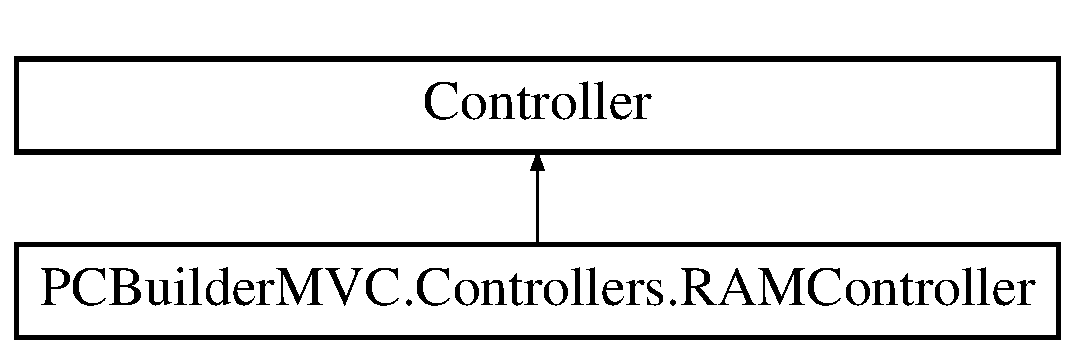
\includegraphics[height=2.000000cm]{class_p_c_builder_m_v_c_1_1_controllers_1_1_r_a_m_controller}
\end{center}
\end{figure}
\subsection*{Public Member Functions}
\begin{DoxyCompactItemize}
\item 
Action\+Result {\bfseries Index} ()\hypertarget{class_p_c_builder_m_v_c_1_1_controllers_1_1_r_a_m_controller_ab5f0288624ca2c326259e9224b2dfdf3}{}\label{class_p_c_builder_m_v_c_1_1_controllers_1_1_r_a_m_controller_ab5f0288624ca2c326259e9224b2dfdf3}

\item 
Action\+Result {\bfseries Details} (int?id)\hypertarget{class_p_c_builder_m_v_c_1_1_controllers_1_1_r_a_m_controller_a565ca84426d8a94125ff0ba785b41141}{}\label{class_p_c_builder_m_v_c_1_1_controllers_1_1_r_a_m_controller_a565ca84426d8a94125ff0ba785b41141}

\item 
Action\+Result {\bfseries Create} ()\hypertarget{class_p_c_builder_m_v_c_1_1_controllers_1_1_r_a_m_controller_a893128c612df2fafac1d8562317965f0}{}\label{class_p_c_builder_m_v_c_1_1_controllers_1_1_r_a_m_controller_a893128c612df2fafac1d8562317965f0}

\item 
Action\+Result {\bfseries Create} (\mbox{[}Bind(Include=\char`\"{}Ram\+Id,Brand,Model,Ram\+Size,Ram\+Generation,Ram\+Speed,Ram\+Timings,Best\+Use,Price\char`\"{})\mbox{]} R\+AM r\+AM)\hypertarget{class_p_c_builder_m_v_c_1_1_controllers_1_1_r_a_m_controller_af78cd8b7deadb2481e69f886a6b7ef8d}{}\label{class_p_c_builder_m_v_c_1_1_controllers_1_1_r_a_m_controller_af78cd8b7deadb2481e69f886a6b7ef8d}

\item 
Action\+Result {\bfseries Edit} (int?id)\hypertarget{class_p_c_builder_m_v_c_1_1_controllers_1_1_r_a_m_controller_a78e10f8249868635dcfa1f0683330b44}{}\label{class_p_c_builder_m_v_c_1_1_controllers_1_1_r_a_m_controller_a78e10f8249868635dcfa1f0683330b44}

\item 
Action\+Result {\bfseries Edit} (\mbox{[}Bind(Include=\char`\"{}Ram\+Id,Brand,Model,Ram\+Size,Ram\+Generation,Ram\+Speed,Ram\+Timings,Best\+Use,Price\char`\"{})\mbox{]} R\+AM r\+AM)\hypertarget{class_p_c_builder_m_v_c_1_1_controllers_1_1_r_a_m_controller_ae754b5e8f84669b8c05909c0571e7e10}{}\label{class_p_c_builder_m_v_c_1_1_controllers_1_1_r_a_m_controller_ae754b5e8f84669b8c05909c0571e7e10}

\item 
Action\+Result {\bfseries Delete} (int?id)\hypertarget{class_p_c_builder_m_v_c_1_1_controllers_1_1_r_a_m_controller_a2f5ad983c778bfa1bf98f733fc28bc9e}{}\label{class_p_c_builder_m_v_c_1_1_controllers_1_1_r_a_m_controller_a2f5ad983c778bfa1bf98f733fc28bc9e}

\item 
Action\+Result {\bfseries Delete\+Confirmed} (int id)\hypertarget{class_p_c_builder_m_v_c_1_1_controllers_1_1_r_a_m_controller_a2d3ebd51384824c662b8f0a3b32db293}{}\label{class_p_c_builder_m_v_c_1_1_controllers_1_1_r_a_m_controller_a2d3ebd51384824c662b8f0a3b32db293}

\end{DoxyCompactItemize}
\subsection*{Protected Member Functions}
\begin{DoxyCompactItemize}
\item 
override void {\bfseries Dispose} (bool disposing)\hypertarget{class_p_c_builder_m_v_c_1_1_controllers_1_1_r_a_m_controller_a8c08e16079a01fff70e528def1005323}{}\label{class_p_c_builder_m_v_c_1_1_controllers_1_1_r_a_m_controller_a8c08e16079a01fff70e528def1005323}

\end{DoxyCompactItemize}
\subsection*{Private Attributes}
\begin{DoxyCompactItemize}
\item 
\hyperlink{class_p_c_builder_m_v_c_1_1_models_1_1_p_c_builder_entity_models}{P\+C\+Builder\+Entity\+Models} {\bfseries db} = new \hyperlink{class_p_c_builder_m_v_c_1_1_models_1_1_p_c_builder_entity_models}{P\+C\+Builder\+Entity\+Models}()\hypertarget{class_p_c_builder_m_v_c_1_1_controllers_1_1_r_a_m_controller_a6134de9d72d65071465e49a3f52e7f83}{}\label{class_p_c_builder_m_v_c_1_1_controllers_1_1_r_a_m_controller_a6134de9d72d65071465e49a3f52e7f83}

\end{DoxyCompactItemize}


\subsection{Detailed Description}
R\+AM controller class to handle R\+AM views interaction. 

\begin{DoxySeeAlso}{See also}
System.\+Web.\+Mvc.\+Controller


\end{DoxySeeAlso}


Definition at line 17 of file R\+A\+M\+Controller.\+cs.



The documentation for this class was generated from the following file\+:\begin{DoxyCompactItemize}
\item 
C\+:/\+Users/nh228u08/\+Desktop/\+Final\+Project/\+Final\+Project/\+P\+C\+Builder/\+P\+C\+Builder\+M\+V\+C/\+Controllers/R\+A\+M\+Controller.\+cs\end{DoxyCompactItemize}

\hypertarget{class_p_c_builder_m_v_c_1_1_models_1_1_register_view_model}{}\section{P\+C\+Builder\+M\+V\+C.\+Models.\+Register\+View\+Model Class Reference}
\label{class_p_c_builder_m_v_c_1_1_models_1_1_register_view_model}\index{P\+C\+Builder\+M\+V\+C.\+Models.\+Register\+View\+Model@{P\+C\+Builder\+M\+V\+C.\+Models.\+Register\+View\+Model}}


Register view model class.  


\subsection*{Properties}
\begin{DoxyCompactItemize}
\item 
string {\bfseries Email}\hspace{0.3cm}{\ttfamily  \mbox{[}get, set\mbox{]}}\hypertarget{class_p_c_builder_m_v_c_1_1_models_1_1_register_view_model_af8ae2184f403e620de3d21ae932d1b0e}{}\label{class_p_c_builder_m_v_c_1_1_models_1_1_register_view_model_af8ae2184f403e620de3d21ae932d1b0e}

\item 
string {\bfseries Password}\hspace{0.3cm}{\ttfamily  \mbox{[}get, set\mbox{]}}\hypertarget{class_p_c_builder_m_v_c_1_1_models_1_1_register_view_model_a589ad6550bb3e870c0133b5065ea785a}{}\label{class_p_c_builder_m_v_c_1_1_models_1_1_register_view_model_a589ad6550bb3e870c0133b5065ea785a}

\item 
string {\bfseries Confirm\+Password}\hspace{0.3cm}{\ttfamily  \mbox{[}get, set\mbox{]}}\hypertarget{class_p_c_builder_m_v_c_1_1_models_1_1_register_view_model_aac262891062b5be4831f40a4baf06f48}{}\label{class_p_c_builder_m_v_c_1_1_models_1_1_register_view_model_aac262891062b5be4831f40a4baf06f48}

\end{DoxyCompactItemize}


\subsection{Detailed Description}
Register view model class. 



Definition at line 69 of file Account\+View\+Models.\+cs.



The documentation for this class was generated from the following file\+:\begin{DoxyCompactItemize}
\item 
C\+:/\+Users/nh228u08/\+Desktop/\+Final\+Project/\+Final\+Project/\+P\+C\+Builder/\+P\+C\+Builder\+M\+V\+C/\+Models/Account\+View\+Models.\+cs\end{DoxyCompactItemize}

\hypertarget{class_p_c_builder_m_v_c_1_1_models_1_1_reset_password_view_model}{}\section{P\+C\+Builder\+M\+V\+C.\+Models.\+Reset\+Password\+View\+Model Class Reference}
\label{class_p_c_builder_m_v_c_1_1_models_1_1_reset_password_view_model}\index{P\+C\+Builder\+M\+V\+C.\+Models.\+Reset\+Password\+View\+Model@{P\+C\+Builder\+M\+V\+C.\+Models.\+Reset\+Password\+View\+Model}}


Reset password view model class.  


\subsection*{Properties}
\begin{DoxyCompactItemize}
\item 
string {\bfseries Email}\hspace{0.3cm}{\ttfamily  \mbox{[}get, set\mbox{]}}\hypertarget{class_p_c_builder_m_v_c_1_1_models_1_1_reset_password_view_model_a2c53540b3481e1994ee9ad64750a806e}{}\label{class_p_c_builder_m_v_c_1_1_models_1_1_reset_password_view_model_a2c53540b3481e1994ee9ad64750a806e}

\item 
string {\bfseries Password}\hspace{0.3cm}{\ttfamily  \mbox{[}get, set\mbox{]}}\hypertarget{class_p_c_builder_m_v_c_1_1_models_1_1_reset_password_view_model_a4d34cb18a2718e42fc07d4ee2f8135a0}{}\label{class_p_c_builder_m_v_c_1_1_models_1_1_reset_password_view_model_a4d34cb18a2718e42fc07d4ee2f8135a0}

\item 
string {\bfseries Confirm\+Password}\hspace{0.3cm}{\ttfamily  \mbox{[}get, set\mbox{]}}\hypertarget{class_p_c_builder_m_v_c_1_1_models_1_1_reset_password_view_model_a0630c820b7c3f9b1e38a9740c2afb7b7}{}\label{class_p_c_builder_m_v_c_1_1_models_1_1_reset_password_view_model_a0630c820b7c3f9b1e38a9740c2afb7b7}

\item 
string {\bfseries Code}\hspace{0.3cm}{\ttfamily  \mbox{[}get, set\mbox{]}}\hypertarget{class_p_c_builder_m_v_c_1_1_models_1_1_reset_password_view_model_a909fa9be9e4d1f30a709ffed921f5239}{}\label{class_p_c_builder_m_v_c_1_1_models_1_1_reset_password_view_model_a909fa9be9e4d1f30a709ffed921f5239}

\end{DoxyCompactItemize}


\subsection{Detailed Description}
Reset password view model class. 



Definition at line 91 of file Account\+View\+Models.\+cs.



The documentation for this class was generated from the following file\+:\begin{DoxyCompactItemize}
\item 
C\+:/\+Users/nh228u08/\+Desktop/\+Final\+Project/\+Final\+Project/\+P\+C\+Builder/\+P\+C\+Builder\+M\+V\+C/\+Models/Account\+View\+Models.\+cs\end{DoxyCompactItemize}

\hypertarget{class_p_c_builder_forms_1_1_properties_1_1_resources}{}\section{P\+C\+Builder\+Forms.\+Properties.\+Resources Class Reference}
\label{class_p_c_builder_forms_1_1_properties_1_1_resources}\index{P\+C\+Builder\+Forms.\+Properties.\+Resources@{P\+C\+Builder\+Forms.\+Properties.\+Resources}}


A strongly-\/typed resource class, for looking up localized strings, etc.  


\subsection*{Properties}
\begin{DoxyCompactItemize}
\item 
static global\+::\+System.\+Resources.\+Resource\+Manager \hyperlink{class_p_c_builder_forms_1_1_properties_1_1_resources_ac6548299b72ecf6fdd7e522ea4c49acf}{Resource\+Manager}\hspace{0.3cm}{\ttfamily  \mbox{[}get\mbox{]}}
\begin{DoxyCompactList}\small\item\em Returns the cached Resource\+Manager instance used by this class. \end{DoxyCompactList}\item 
static global\+::\+System.\+Globalization.\+Culture\+Info \hyperlink{class_p_c_builder_forms_1_1_properties_1_1_resources_a815a910fd4361950f9ebd6fcf6209cc8}{Culture}\hspace{0.3cm}{\ttfamily  \mbox{[}get, set\mbox{]}}
\begin{DoxyCompactList}\small\item\em Overrides the current thread\textquotesingle{}s Current\+U\+I\+Culture property for all resource lookups using this strongly typed resource class. \end{DoxyCompactList}\end{DoxyCompactItemize}
\subsection*{Static Private Attributes}
\begin{DoxyCompactItemize}
\item 
static global\+::\+System.\+Resources.\+Resource\+Manager {\bfseries resource\+Man}\hypertarget{class_p_c_builder_forms_1_1_properties_1_1_resources_ae7b01286aebde33d034035d1aaf42800}{}\label{class_p_c_builder_forms_1_1_properties_1_1_resources_ae7b01286aebde33d034035d1aaf42800}

\item 
static global\+::\+System.\+Globalization.\+Culture\+Info {\bfseries resource\+Culture}\hypertarget{class_p_c_builder_forms_1_1_properties_1_1_resources_af671e11dd336cdd0e0cb6d270fb48704}{}\label{class_p_c_builder_forms_1_1_properties_1_1_resources_af671e11dd336cdd0e0cb6d270fb48704}

\end{DoxyCompactItemize}


\subsection{Detailed Description}
A strongly-\/typed resource class, for looking up localized strings, etc. 



Definition at line 25 of file Resources.\+Designer.\+cs.



\subsection{Property Documentation}
\index{P\+C\+Builder\+Forms\+::\+Properties\+::\+Resources@{P\+C\+Builder\+Forms\+::\+Properties\+::\+Resources}!Culture@{Culture}}
\index{Culture@{Culture}!P\+C\+Builder\+Forms\+::\+Properties\+::\+Resources@{P\+C\+Builder\+Forms\+::\+Properties\+::\+Resources}}
\subsubsection[{\texorpdfstring{Culture}{Culture}}]{\setlength{\rightskip}{0pt plus 5cm}global.\+System.\+Globalization.\+Culture\+Info P\+C\+Builder\+Forms.\+Properties.\+Resources.\+Culture\hspace{0.3cm}{\ttfamily [static]}, {\ttfamily [get]}, {\ttfamily [set]}, {\ttfamily [package]}}\hypertarget{class_p_c_builder_forms_1_1_properties_1_1_resources_a815a910fd4361950f9ebd6fcf6209cc8}{}\label{class_p_c_builder_forms_1_1_properties_1_1_resources_a815a910fd4361950f9ebd6fcf6209cc8}


Overrides the current thread\textquotesingle{}s Current\+U\+I\+Culture property for all resource lookups using this strongly typed resource class. 



Definition at line 60 of file Resources.\+Designer.\+cs.

\index{P\+C\+Builder\+Forms\+::\+Properties\+::\+Resources@{P\+C\+Builder\+Forms\+::\+Properties\+::\+Resources}!Resource\+Manager@{Resource\+Manager}}
\index{Resource\+Manager@{Resource\+Manager}!P\+C\+Builder\+Forms\+::\+Properties\+::\+Resources@{P\+C\+Builder\+Forms\+::\+Properties\+::\+Resources}}
\subsubsection[{\texorpdfstring{Resource\+Manager}{ResourceManager}}]{\setlength{\rightskip}{0pt plus 5cm}global.\+System.\+Resources.\+Resource\+Manager P\+C\+Builder\+Forms.\+Properties.\+Resources.\+Resource\+Manager\hspace{0.3cm}{\ttfamily [static]}, {\ttfamily [get]}, {\ttfamily [package]}}\hypertarget{class_p_c_builder_forms_1_1_properties_1_1_resources_ac6548299b72ecf6fdd7e522ea4c49acf}{}\label{class_p_c_builder_forms_1_1_properties_1_1_resources_ac6548299b72ecf6fdd7e522ea4c49acf}


Returns the cached Resource\+Manager instance used by this class. 



Definition at line 42 of file Resources.\+Designer.\+cs.



The documentation for this class was generated from the following file\+:\begin{DoxyCompactItemize}
\item 
C\+:/\+Users/nh228u08/\+Desktop/\+Final\+Project/\+Final\+Project/\+P\+C\+Builder/\+P\+C\+Builder\+Forms/\+Properties/Resources.\+Designer.\+cs\end{DoxyCompactItemize}

\hypertarget{class_p_c_builder_m_v_c_1_1_models_1_1_role}{}\section{P\+C\+Builder\+M\+V\+C.\+Models.\+Role Class Reference}
\label{class_p_c_builder_m_v_c_1_1_models_1_1_role}\index{P\+C\+Builder\+M\+V\+C.\+Models.\+Role@{P\+C\+Builder\+M\+V\+C.\+Models.\+Role}}


\hyperlink{class_p_c_builder_m_v_c_1_1_models_1_1_role}{Role} view model class.  


\subsection*{Properties}
\begin{DoxyCompactItemize}
\item 
int {\bfseries Role\+Id}\hspace{0.3cm}{\ttfamily  \mbox{[}get, set\mbox{]}}\hypertarget{class_p_c_builder_m_v_c_1_1_models_1_1_role_a54894e076feb6b9c47bc35b80852f10f}{}\label{class_p_c_builder_m_v_c_1_1_models_1_1_role_a54894e076feb6b9c47bc35b80852f10f}

\item 
string {\bfseries Role\+Name}\hspace{0.3cm}{\ttfamily  \mbox{[}get, set\mbox{]}}\hypertarget{class_p_c_builder_m_v_c_1_1_models_1_1_role_ae256433056a0fe154c30f4a5f3ab3c9e}{}\label{class_p_c_builder_m_v_c_1_1_models_1_1_role_ae256433056a0fe154c30f4a5f3ab3c9e}

\item 
string {\bfseries Role\+Description}\hspace{0.3cm}{\ttfamily  \mbox{[}get, set\mbox{]}}\hypertarget{class_p_c_builder_m_v_c_1_1_models_1_1_role_a4c00642714f2e84604864cb2c7d91e8c}{}\label{class_p_c_builder_m_v_c_1_1_models_1_1_role_a4c00642714f2e84604864cb2c7d91e8c}

\end{DoxyCompactItemize}


\subsection{Detailed Description}
\hyperlink{class_p_c_builder_m_v_c_1_1_models_1_1_role}{Role} view model class. 



Definition at line 13 of file Role.\+cs.



The documentation for this class was generated from the following file\+:\begin{DoxyCompactItemize}
\item 
C\+:/\+Users/nh228u08/\+Desktop/\+Final\+Project/\+Final\+Project/\+P\+C\+Builder/\+P\+C\+Builder\+M\+V\+C/\+Models/Role.\+cs\end{DoxyCompactItemize}

\hypertarget{class_p_c_builder_m_v_c_1_1_controllers_1_1_role_controller}{}\section{P\+C\+Builder\+M\+V\+C.\+Controllers.\+Role\+Controller Class Reference}
\label{class_p_c_builder_m_v_c_1_1_controllers_1_1_role_controller}\index{P\+C\+Builder\+M\+V\+C.\+Controllers.\+Role\+Controller@{P\+C\+Builder\+M\+V\+C.\+Controllers.\+Role\+Controller}}


Role controller class to handle Role views interaction.  


Inheritance diagram for P\+C\+Builder\+M\+V\+C.\+Controllers.\+Role\+Controller\+:\begin{figure}[H]
\begin{center}
\leavevmode
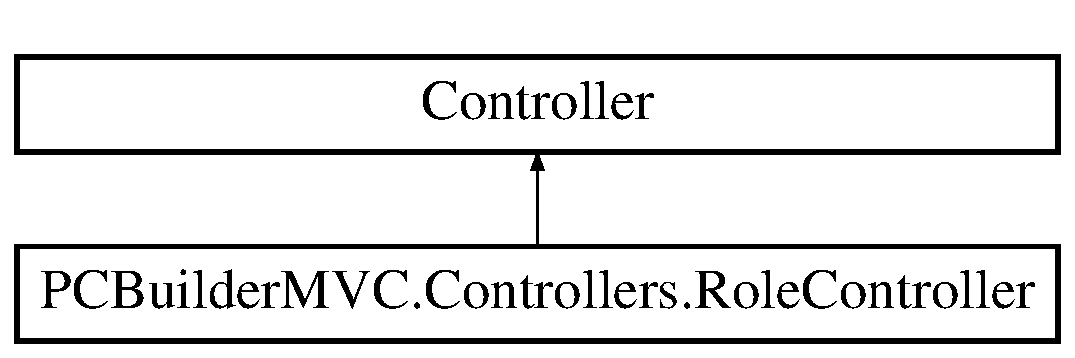
\includegraphics[height=2.000000cm]{class_p_c_builder_m_v_c_1_1_controllers_1_1_role_controller}
\end{center}
\end{figure}
\subsection*{Public Member Functions}
\begin{DoxyCompactItemize}
\item 
Action\+Result {\bfseries Index} ()\hypertarget{class_p_c_builder_m_v_c_1_1_controllers_1_1_role_controller_a539d1b8b95c8cce64e2e6191070ab4f1}{}\label{class_p_c_builder_m_v_c_1_1_controllers_1_1_role_controller_a539d1b8b95c8cce64e2e6191070ab4f1}

\item 
Action\+Result {\bfseries Details} (int?id)\hypertarget{class_p_c_builder_m_v_c_1_1_controllers_1_1_role_controller_a622d75d4760677d73ecef02d8b7e4112}{}\label{class_p_c_builder_m_v_c_1_1_controllers_1_1_role_controller_a622d75d4760677d73ecef02d8b7e4112}

\item 
Action\+Result {\bfseries Create} ()\hypertarget{class_p_c_builder_m_v_c_1_1_controllers_1_1_role_controller_ac7d1a9619975e3e734535a104731fab4}{}\label{class_p_c_builder_m_v_c_1_1_controllers_1_1_role_controller_ac7d1a9619975e3e734535a104731fab4}

\item 
Action\+Result {\bfseries Create} (\mbox{[}Bind(Include=\char`\"{}Role\+Id,Role\+Name,Role\+Description\char`\"{})\mbox{]} Role role)\hypertarget{class_p_c_builder_m_v_c_1_1_controllers_1_1_role_controller_a380152084b9a7911121f64f4c7890c53}{}\label{class_p_c_builder_m_v_c_1_1_controllers_1_1_role_controller_a380152084b9a7911121f64f4c7890c53}

\item 
Action\+Result {\bfseries Edit} (int?id)\hypertarget{class_p_c_builder_m_v_c_1_1_controllers_1_1_role_controller_acfe183da8623b0e5ceaa1e345b78c83f}{}\label{class_p_c_builder_m_v_c_1_1_controllers_1_1_role_controller_acfe183da8623b0e5ceaa1e345b78c83f}

\item 
Action\+Result {\bfseries Edit} (\mbox{[}Bind(Include=\char`\"{}Role\+Id,Role\+Name,Role\+Description\char`\"{})\mbox{]} Role role)\hypertarget{class_p_c_builder_m_v_c_1_1_controllers_1_1_role_controller_a7726bbef911a2d11d6dd051a1ad336be}{}\label{class_p_c_builder_m_v_c_1_1_controllers_1_1_role_controller_a7726bbef911a2d11d6dd051a1ad336be}

\item 
Action\+Result {\bfseries Delete} (int?id)\hypertarget{class_p_c_builder_m_v_c_1_1_controllers_1_1_role_controller_a9b8397f06d1f42fa5aca85d14d9ac8cf}{}\label{class_p_c_builder_m_v_c_1_1_controllers_1_1_role_controller_a9b8397f06d1f42fa5aca85d14d9ac8cf}

\item 
Action\+Result {\bfseries Delete\+Confirmed} (int id)\hypertarget{class_p_c_builder_m_v_c_1_1_controllers_1_1_role_controller_a9f7f7bd802c01e7fd33c2d5b14b7ca3e}{}\label{class_p_c_builder_m_v_c_1_1_controllers_1_1_role_controller_a9f7f7bd802c01e7fd33c2d5b14b7ca3e}

\end{DoxyCompactItemize}
\subsection*{Protected Member Functions}
\begin{DoxyCompactItemize}
\item 
override void {\bfseries Dispose} (bool disposing)\hypertarget{class_p_c_builder_m_v_c_1_1_controllers_1_1_role_controller_a6c4e2e6ec3e29a8c899cd71da1450150}{}\label{class_p_c_builder_m_v_c_1_1_controllers_1_1_role_controller_a6c4e2e6ec3e29a8c899cd71da1450150}

\end{DoxyCompactItemize}
\subsection*{Private Attributes}
\begin{DoxyCompactItemize}
\item 
\hyperlink{class_p_c_builder_m_v_c_1_1_models_1_1_p_c_builder_entity_models}{P\+C\+Builder\+Entity\+Models} {\bfseries db} = new \hyperlink{class_p_c_builder_m_v_c_1_1_models_1_1_p_c_builder_entity_models}{P\+C\+Builder\+Entity\+Models}()\hypertarget{class_p_c_builder_m_v_c_1_1_controllers_1_1_role_controller_a80a5f7cc23a5d4f5b44003861bc251c0}{}\label{class_p_c_builder_m_v_c_1_1_controllers_1_1_role_controller_a80a5f7cc23a5d4f5b44003861bc251c0}

\end{DoxyCompactItemize}


\subsection{Detailed Description}
Role controller class to handle Role views interaction. 

\begin{DoxySeeAlso}{See also}
System.\+Web.\+Mvc.\+Controller


\end{DoxySeeAlso}


Definition at line 17 of file Role\+Controller.\+cs.



The documentation for this class was generated from the following file\+:\begin{DoxyCompactItemize}
\item 
C\+:/\+Users/nh228u08/\+Desktop/\+Final\+Project/\+Final\+Project/\+P\+C\+Builder/\+P\+C\+Builder\+M\+V\+C/\+Controllers/Role\+Controller.\+cs\end{DoxyCompactItemize}

\hypertarget{class_business_objects_1_1_roles}{}\section{Business\+Objects.\+Roles Class Reference}
\label{class_business_objects_1_1_roles}\index{Business\+Objects.\+Roles@{Business\+Objects.\+Roles}}


Role class that holds a role property.  


\subsection*{Properties}
\begin{DoxyCompactItemize}
\item 
string \hyperlink{class_business_objects_1_1_roles_ac3d92844ec99b3c5d19117a5d110c1fd}{Role}\hspace{0.3cm}{\ttfamily  \mbox{[}get, set\mbox{]}}
\begin{DoxyCompactList}\small\item\em Gets or sets the role. \end{DoxyCompactList}\end{DoxyCompactItemize}


\subsection{Detailed Description}
Role class that holds a role property. 



Definition at line 12 of file Roles.\+cs.



\subsection{Property Documentation}
\index{Business\+Objects\+::\+Roles@{Business\+Objects\+::\+Roles}!Role@{Role}}
\index{Role@{Role}!Business\+Objects\+::\+Roles@{Business\+Objects\+::\+Roles}}
\subsubsection[{\texorpdfstring{Role}{Role}}]{\setlength{\rightskip}{0pt plus 5cm}string Business\+Objects.\+Roles.\+Role\hspace{0.3cm}{\ttfamily [get]}, {\ttfamily [set]}}\hypertarget{class_business_objects_1_1_roles_ac3d92844ec99b3c5d19117a5d110c1fd}{}\label{class_business_objects_1_1_roles_ac3d92844ec99b3c5d19117a5d110c1fd}


Gets or sets the role. 

The role. 

Definition at line 20 of file Roles.\+cs.



The documentation for this class was generated from the following file\+:\begin{DoxyCompactItemize}
\item 
C\+:/\+Users/nh228u08/\+Desktop/\+Final\+Project/\+Final\+Project/\+P\+C\+Builder/\+Business\+Objects/Roles.\+cs\end{DoxyCompactItemize}

\hypertarget{class_p_c_builder_m_v_c_1_1_route_config}{}\section{P\+C\+Builder\+M\+V\+C.\+Route\+Config Class Reference}
\label{class_p_c_builder_m_v_c_1_1_route_config}\index{P\+C\+Builder\+M\+V\+C.\+Route\+Config@{P\+C\+Builder\+M\+V\+C.\+Route\+Config}}


Path configuration for M\+VC.  


\subsection*{Static Public Member Functions}
\begin{DoxyCompactItemize}
\item 
static void \hyperlink{class_p_c_builder_m_v_c_1_1_route_config_a3b8e090f16c0cbc87086f988712d0480}{Register\+Routes} (Route\+Collection routes)
\begin{DoxyCompactList}\small\item\em Registers the routes. \end{DoxyCompactList}\end{DoxyCompactItemize}


\subsection{Detailed Description}
Path configuration for M\+VC. 



Definition at line 13 of file Route\+Config.\+cs.



\subsection{Member Function Documentation}
\index{P\+C\+Builder\+M\+V\+C\+::\+Route\+Config@{P\+C\+Builder\+M\+V\+C\+::\+Route\+Config}!Register\+Routes@{Register\+Routes}}
\index{Register\+Routes@{Register\+Routes}!P\+C\+Builder\+M\+V\+C\+::\+Route\+Config@{P\+C\+Builder\+M\+V\+C\+::\+Route\+Config}}
\subsubsection[{\texorpdfstring{Register\+Routes(\+Route\+Collection routes)}{RegisterRoutes(RouteCollection routes)}}]{\setlength{\rightskip}{0pt plus 5cm}static void P\+C\+Builder\+M\+V\+C.\+Route\+Config.\+Register\+Routes (
\begin{DoxyParamCaption}
\item[{Route\+Collection}]{routes}
\end{DoxyParamCaption}
)\hspace{0.3cm}{\ttfamily [static]}}\hypertarget{class_p_c_builder_m_v_c_1_1_route_config_a3b8e090f16c0cbc87086f988712d0480}{}\label{class_p_c_builder_m_v_c_1_1_route_config_a3b8e090f16c0cbc87086f988712d0480}


Registers the routes. 


\begin{DoxyParams}{Parameters}
{\em routes} & The routes.\\
\hline
\end{DoxyParams}


Definition at line 19 of file Route\+Config.\+cs.



The documentation for this class was generated from the following file\+:\begin{DoxyCompactItemize}
\item 
C\+:/\+Users/nh228u08/\+Desktop/\+Final\+Project/\+Final\+Project/\+P\+C\+Builder/\+P\+C\+Builder\+M\+V\+C/\+App\+\_\+\+Start/Route\+Config.\+cs\end{DoxyCompactItemize}

\hypertarget{class_business_logic_1_1_security_manager}{}\section{Business\+Logic.\+Security\+Manager Class Reference}
\label{class_business_logic_1_1_security_manager}\index{Business\+Logic.\+Security\+Manager@{Business\+Logic.\+Security\+Manager}}


Class tasked with maintaining application security when handling user information.  


\subsection*{Static Public Member Functions}
\begin{DoxyCompactItemize}
\item 
static \hyperlink{class_business_objects_1_1_access_token}{Access\+Token} \hyperlink{class_business_logic_1_1_security_manager_a27a0b4ffd4af28d8ccdf5751b2bc0445}{Validate\+Existing\+User} (string username, string password)
\begin{DoxyCompactList}\small\item\em Validates an existing user. \end{DoxyCompactList}\item 
static \hyperlink{class_business_objects_1_1_access_token}{Access\+Token} \hyperlink{class_business_logic_1_1_security_manager_a88cf89e8c9ad9e7b34a8e7525fcf5f84}{Validate\+New\+User} (\hyperlink{class_business_objects_1_1_user}{User} usr)
\begin{DoxyCompactList}\small\item\em Validates a new user. \end{DoxyCompactList}\end{DoxyCompactItemize}
\subsection*{Private Attributes}
\begin{DoxyCompactItemize}
\item 
const int {\bfseries M\+I\+N\+\_\+\+U\+S\+E\+R\+N\+A\+ME} = 5\hypertarget{class_business_logic_1_1_security_manager_ae23ca68a4b39e825dd84c625507c3bab}{}\label{class_business_logic_1_1_security_manager_ae23ca68a4b39e825dd84c625507c3bab}

\item 
const int {\bfseries M\+I\+N\+\_\+\+P\+A\+S\+S\+W\+O\+RD} = 5\hypertarget{class_business_logic_1_1_security_manager_a5e99763198398db090c6211c5158acd4}{}\label{class_business_logic_1_1_security_manager_a5e99763198398db090c6211c5158acd4}

\end{DoxyCompactItemize}


\subsection{Detailed Description}
Class tasked with maintaining application security when handling user information. 



Definition at line 14 of file Security\+Manager.\+cs.



\subsection{Member Function Documentation}
\index{Business\+Logic\+::\+Security\+Manager@{Business\+Logic\+::\+Security\+Manager}!Validate\+Existing\+User@{Validate\+Existing\+User}}
\index{Validate\+Existing\+User@{Validate\+Existing\+User}!Business\+Logic\+::\+Security\+Manager@{Business\+Logic\+::\+Security\+Manager}}
\subsubsection[{\texorpdfstring{Validate\+Existing\+User(string username, string password)}{ValidateExistingUser(string username, string password)}}]{\setlength{\rightskip}{0pt plus 5cm}static {\bf Access\+Token} Business\+Logic.\+Security\+Manager.\+Validate\+Existing\+User (
\begin{DoxyParamCaption}
\item[{string}]{username, }
\item[{string}]{password}
\end{DoxyParamCaption}
)\hspace{0.3cm}{\ttfamily [static]}}\hypertarget{class_business_logic_1_1_security_manager_a27a0b4ffd4af28d8ccdf5751b2bc0445}{}\label{class_business_logic_1_1_security_manager_a27a0b4ffd4af28d8ccdf5751b2bc0445}


Validates an existing user. 


\begin{DoxyParams}{Parameters}
{\em username} & The username.\\
\hline
{\em password} & The password.\\
\hline
\end{DoxyParams}
\begin{DoxyReturn}{Returns}
Access\+Token used to keep validated information for processing.
\end{DoxyReturn}

\begin{DoxyExceptions}{Exceptions}
{\em System.\+Application\+Exception} & Password and username must be between 5 and 50 characters. or Data not found. \\
\hline
\end{DoxyExceptions}


Definition at line 30 of file Security\+Manager.\+cs.

\index{Business\+Logic\+::\+Security\+Manager@{Business\+Logic\+::\+Security\+Manager}!Validate\+New\+User@{Validate\+New\+User}}
\index{Validate\+New\+User@{Validate\+New\+User}!Business\+Logic\+::\+Security\+Manager@{Business\+Logic\+::\+Security\+Manager}}
\subsubsection[{\texorpdfstring{Validate\+New\+User(\+User usr)}{ValidateNewUser(User usr)}}]{\setlength{\rightskip}{0pt plus 5cm}static {\bf Access\+Token} Business\+Logic.\+Security\+Manager.\+Validate\+New\+User (
\begin{DoxyParamCaption}
\item[{{\bf User}}]{usr}
\end{DoxyParamCaption}
)\hspace{0.3cm}{\ttfamily [static]}}\hypertarget{class_business_logic_1_1_security_manager_a88cf89e8c9ad9e7b34a8e7525fcf5f84}{}\label{class_business_logic_1_1_security_manager_a88cf89e8c9ad9e7b34a8e7525fcf5f84}


Validates a new user. 


\begin{DoxyParams}{Parameters}
{\em usr} & The user.\\
\hline
\end{DoxyParams}
\begin{DoxyReturn}{Returns}
Access\+Token used to keep validated information for processing.
\end{DoxyReturn}

\begin{DoxyExceptions}{Exceptions}
{\em System.\+Application\+Exception} & User already exists!\\
\hline
\end{DoxyExceptions}


Definition at line 66 of file Security\+Manager.\+cs.



The documentation for this class was generated from the following file\+:\begin{DoxyCompactItemize}
\item 
C\+:/\+Users/nh228u08/\+Desktop/\+Final\+Project/\+Final\+Project/\+P\+C\+Builder/\+Business\+Logic/Security\+Manager.\+cs\end{DoxyCompactItemize}

\hypertarget{class_p_c_builder_forms_1_1_properties_1_1_settings}{}\section{P\+C\+Builder\+Forms.\+Properties.\+Settings Class Reference}
\label{class_p_c_builder_forms_1_1_properties_1_1_settings}\index{P\+C\+Builder\+Forms.\+Properties.\+Settings@{P\+C\+Builder\+Forms.\+Properties.\+Settings}}
Inheritance diagram for P\+C\+Builder\+Forms.\+Properties.\+Settings\+:\begin{figure}[H]
\begin{center}
\leavevmode
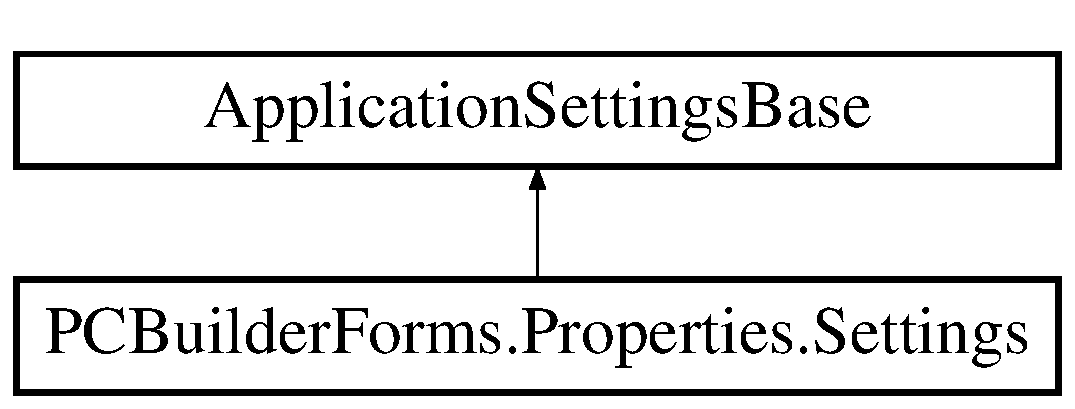
\includegraphics[height=2.000000cm]{class_p_c_builder_forms_1_1_properties_1_1_settings}
\end{center}
\end{figure}
\subsection*{Properties}
\begin{DoxyCompactItemize}
\item 
static \hyperlink{class_p_c_builder_forms_1_1_properties_1_1_settings}{Settings} {\bfseries Default}\hspace{0.3cm}{\ttfamily  \mbox{[}get\mbox{]}}\hypertarget{class_p_c_builder_forms_1_1_properties_1_1_settings_ab249d99921408a81b2f5b75c0945e547}{}\label{class_p_c_builder_forms_1_1_properties_1_1_settings_ab249d99921408a81b2f5b75c0945e547}

\end{DoxyCompactItemize}
\subsection*{Static Private Attributes}
\begin{DoxyCompactItemize}
\item 
static \hyperlink{class_p_c_builder_forms_1_1_properties_1_1_settings}{Settings} {\bfseries default\+Instance} = ((\hyperlink{class_p_c_builder_forms_1_1_properties_1_1_settings}{Settings})(global\+::\+System.\+Configuration.\+Application\+Settings\+Base.\+Synchronized(new \hyperlink{class_p_c_builder_forms_1_1_properties_1_1_settings}{Settings}())))\hypertarget{class_p_c_builder_forms_1_1_properties_1_1_settings_a05f0262a3e60a5088e4bfe2040b999c0}{}\label{class_p_c_builder_forms_1_1_properties_1_1_settings_a05f0262a3e60a5088e4bfe2040b999c0}

\end{DoxyCompactItemize}


\subsection{Detailed Description}


Definition at line 17 of file Settings.\+Designer.\+cs.



The documentation for this class was generated from the following file\+:\begin{DoxyCompactItemize}
\item 
C\+:/\+Users/nh228u08/\+Desktop/\+Final\+Project/\+Final\+Project/\+P\+C\+Builder/\+P\+C\+Builder\+Forms/\+Properties/Settings.\+Designer.\+cs\end{DoxyCompactItemize}

\hypertarget{class_p_c_builder_m_v_c_1_1_sms_service}{}\section{P\+C\+Builder\+M\+V\+C.\+Sms\+Service Class Reference}
\label{class_p_c_builder_m_v_c_1_1_sms_service}\index{P\+C\+Builder\+M\+V\+C.\+Sms\+Service@{P\+C\+Builder\+M\+V\+C.\+Sms\+Service}}


Creates an S\+MS service.  


Inheritance diagram for P\+C\+Builder\+M\+V\+C.\+Sms\+Service\+:\begin{figure}[H]
\begin{center}
\leavevmode
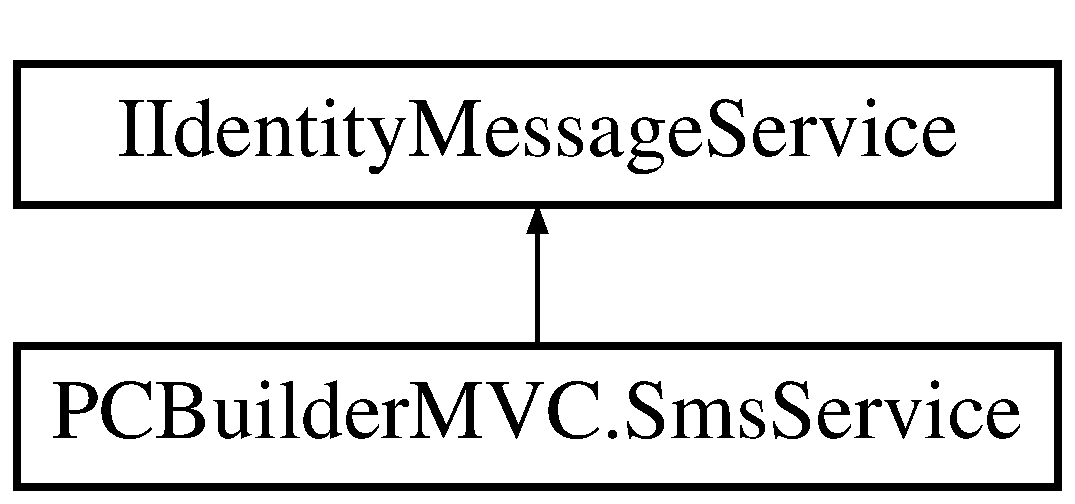
\includegraphics[height=2.000000cm]{class_p_c_builder_m_v_c_1_1_sms_service}
\end{center}
\end{figure}
\subsection*{Public Member Functions}
\begin{DoxyCompactItemize}
\item 
Task {\bfseries Send\+Async} (Identity\+Message message)\hypertarget{class_p_c_builder_m_v_c_1_1_sms_service_afebab35ad2f0bab84e2786ab713907bc}{}\label{class_p_c_builder_m_v_c_1_1_sms_service_afebab35ad2f0bab84e2786ab713907bc}

\end{DoxyCompactItemize}


\subsection{Detailed Description}
Creates an S\+MS service. 

\begin{DoxySeeAlso}{See also}
Microsoft.\+Asp\+Net.\+Identity.\+I\+Identity\+Message\+Service


\end{DoxySeeAlso}


Definition at line 90 of file Identity\+Config.\+cs.



The documentation for this class was generated from the following file\+:\begin{DoxyCompactItemize}
\item 
C\+:/\+Users/nh228u08/\+Desktop/\+Final\+Project/\+Final\+Project/\+P\+C\+Builder/\+P\+C\+Builder\+M\+V\+C/\+App\+\_\+\+Start/Identity\+Config.\+cs\end{DoxyCompactItemize}

\hypertarget{class_business_objects_1_1_standardized_basic}{}\section{Business\+Objects.\+Standardized\+Basic Class Reference}
\label{class_business_objects_1_1_standardized_basic}\index{Business\+Objects.\+Standardized\+Basic@{Business\+Objects.\+Standardized\+Basic}}


Build object to hold necessary data on a Video Editing build.  


\subsection*{Public Member Functions}
\begin{DoxyCompactItemize}
\item 
\hyperlink{class_business_objects_1_1_standardized_basic_a4c81e7aee14a5030d14a336b9ee90605}{Standardized\+Basic} ()
\begin{DoxyCompactList}\small\item\em Initializes a new instance of the \hyperlink{class_business_objects_1_1_standardized_basic}{Standardized\+Basic} class. \end{DoxyCompactList}\end{DoxyCompactItemize}
\subsection*{Public Attributes}
\begin{DoxyCompactItemize}
\item 
\hyperlink{class_business_objects_1_1_c_p_u}{C\+PU} {\bfseries cpu} = new \hyperlink{class_business_objects_1_1_c_p_u}{C\+PU}()\hypertarget{class_business_objects_1_1_standardized_basic_a84f80d9582981524beea065f299ecc35}{}\label{class_business_objects_1_1_standardized_basic_a84f80d9582981524beea065f299ecc35}

\item 
\hyperlink{class_business_objects_1_1_g_p_u}{G\+PU} {\bfseries gpu} = new \hyperlink{class_business_objects_1_1_g_p_u}{G\+PU}()\hypertarget{class_business_objects_1_1_standardized_basic_a4f179bcb04e0cfc171bb8ff448a13550}{}\label{class_business_objects_1_1_standardized_basic_a4f179bcb04e0cfc171bb8ff448a13550}

\item 
\hyperlink{class_business_objects_1_1_motherboard}{Motherboard} {\bfseries motherboard} = new \hyperlink{class_business_objects_1_1_motherboard}{Motherboard}()\hypertarget{class_business_objects_1_1_standardized_basic_a468fce37795574a5e3cd0217ad68208d}{}\label{class_business_objects_1_1_standardized_basic_a468fce37795574a5e3cd0217ad68208d}

\item 
\hyperlink{class_business_objects_1_1_optical}{Optical} {\bfseries optical} = new \hyperlink{class_business_objects_1_1_optical}{Optical}()\hypertarget{class_business_objects_1_1_standardized_basic_a248a04870bc31552cf809b532c2421f1}{}\label{class_business_objects_1_1_standardized_basic_a248a04870bc31552cf809b532c2421f1}

\item 
\hyperlink{class_business_objects_1_1_p_s_u}{P\+SU} {\bfseries psu} = new \hyperlink{class_business_objects_1_1_p_s_u}{P\+SU}()\hypertarget{class_business_objects_1_1_standardized_basic_a49798feb6516066b9637bea9c6d24283}{}\label{class_business_objects_1_1_standardized_basic_a49798feb6516066b9637bea9c6d24283}

\item 
\hyperlink{class_business_objects_1_1_r_a_m}{R\+AM} {\bfseries ram} = new \hyperlink{class_business_objects_1_1_r_a_m}{R\+AM}()\hypertarget{class_business_objects_1_1_standardized_basic_a3467cc8099863b0e31f3a88aed1c05df}{}\label{class_business_objects_1_1_standardized_basic_a3467cc8099863b0e31f3a88aed1c05df}

\item 
\hyperlink{class_business_objects_1_1_storage}{Storage} {\bfseries storage} = new \hyperlink{class_business_objects_1_1_storage}{Storage}()\hypertarget{class_business_objects_1_1_standardized_basic_a0a8504ff7f0f2c2049112dc854dbd221}{}\label{class_business_objects_1_1_standardized_basic_a0a8504ff7f0f2c2049112dc854dbd221}

\end{DoxyCompactItemize}


\subsection{Detailed Description}
Build object to hold necessary data on a Video Editing build. 

This is used as a contingency build if user requests are far too outlandish to create an acceptable build. 

Definition at line 15 of file Standardized\+Basic.\+cs.



\subsection{Constructor \& Destructor Documentation}
\index{Business\+Objects\+::\+Standardized\+Basic@{Business\+Objects\+::\+Standardized\+Basic}!Standardized\+Basic@{Standardized\+Basic}}
\index{Standardized\+Basic@{Standardized\+Basic}!Business\+Objects\+::\+Standardized\+Basic@{Business\+Objects\+::\+Standardized\+Basic}}
\subsubsection[{\texorpdfstring{Standardized\+Basic()}{StandardizedBasic()}}]{\setlength{\rightskip}{0pt plus 5cm}Business\+Objects.\+Standardized\+Basic.\+Standardized\+Basic (
\begin{DoxyParamCaption}
{}
\end{DoxyParamCaption}
)}\hypertarget{class_business_objects_1_1_standardized_basic_a4c81e7aee14a5030d14a336b9ee90605}{}\label{class_business_objects_1_1_standardized_basic_a4c81e7aee14a5030d14a336b9ee90605}


Initializes a new instance of the \hyperlink{class_business_objects_1_1_standardized_basic}{Standardized\+Basic} class. 

Default values are entered into the object at time of instantiation. 

Definition at line 31 of file Standardized\+Basic.\+cs.



The documentation for this class was generated from the following file\+:\begin{DoxyCompactItemize}
\item 
C\+:/\+Users/nh228u08/\+Desktop/\+Final\+Project/\+Final\+Project/\+P\+C\+Builder/\+Business\+Objects/Standardized\+Basic.\+cs\end{DoxyCompactItemize}

\hypertarget{class_business_objects_1_1_standardized_development}{}\section{Business\+Objects.\+Standardized\+Development Class Reference}
\label{class_business_objects_1_1_standardized_development}\index{Business\+Objects.\+Standardized\+Development@{Business\+Objects.\+Standardized\+Development}}


Build object to hold necessary data on a Video Editing build.  


\subsection*{Public Member Functions}
\begin{DoxyCompactItemize}
\item 
\hyperlink{class_business_objects_1_1_standardized_development_a65a94cd1370b7b2abeb84c38fafc8af4}{Standardized\+Development} ()
\begin{DoxyCompactList}\small\item\em Initializes a new instance of the \hyperlink{class_business_objects_1_1_standardized_development}{Standardized\+Development} class. \end{DoxyCompactList}\end{DoxyCompactItemize}
\subsection*{Public Attributes}
\begin{DoxyCompactItemize}
\item 
\hyperlink{class_business_objects_1_1_c_p_u}{C\+PU} {\bfseries cpu} = new \hyperlink{class_business_objects_1_1_c_p_u}{C\+PU}()\hypertarget{class_business_objects_1_1_standardized_development_a5bc2483ecb2c73955f1bd43473a76ba3}{}\label{class_business_objects_1_1_standardized_development_a5bc2483ecb2c73955f1bd43473a76ba3}

\item 
\hyperlink{class_business_objects_1_1_g_p_u}{G\+PU} {\bfseries gpu} = new \hyperlink{class_business_objects_1_1_g_p_u}{G\+PU}()\hypertarget{class_business_objects_1_1_standardized_development_a35a82523bcfbced358a744a2b0aa2973}{}\label{class_business_objects_1_1_standardized_development_a35a82523bcfbced358a744a2b0aa2973}

\item 
\hyperlink{class_business_objects_1_1_motherboard}{Motherboard} {\bfseries motherboard} = new \hyperlink{class_business_objects_1_1_motherboard}{Motherboard}()\hypertarget{class_business_objects_1_1_standardized_development_ad124b8b764cdb5438003cdd3edc54f41}{}\label{class_business_objects_1_1_standardized_development_ad124b8b764cdb5438003cdd3edc54f41}

\item 
\hyperlink{class_business_objects_1_1_optical}{Optical} {\bfseries optical} = new \hyperlink{class_business_objects_1_1_optical}{Optical}()\hypertarget{class_business_objects_1_1_standardized_development_ad66844eb585020b6e83840871dbd34c0}{}\label{class_business_objects_1_1_standardized_development_ad66844eb585020b6e83840871dbd34c0}

\item 
\hyperlink{class_business_objects_1_1_p_s_u}{P\+SU} {\bfseries psu} = new \hyperlink{class_business_objects_1_1_p_s_u}{P\+SU}()\hypertarget{class_business_objects_1_1_standardized_development_a40e64b606dcde9bf0f8ac3258e09a966}{}\label{class_business_objects_1_1_standardized_development_a40e64b606dcde9bf0f8ac3258e09a966}

\item 
\hyperlink{class_business_objects_1_1_r_a_m}{R\+AM} {\bfseries ram} = new \hyperlink{class_business_objects_1_1_r_a_m}{R\+AM}()\hypertarget{class_business_objects_1_1_standardized_development_a2d257a0a8acb247c4230defacf7b991d}{}\label{class_business_objects_1_1_standardized_development_a2d257a0a8acb247c4230defacf7b991d}

\item 
\hyperlink{class_business_objects_1_1_storage}{Storage} {\bfseries storage} = new \hyperlink{class_business_objects_1_1_storage}{Storage}()\hypertarget{class_business_objects_1_1_standardized_development_ae149e2f0d1fea24ee4371cdfb2c62b60}{}\label{class_business_objects_1_1_standardized_development_ae149e2f0d1fea24ee4371cdfb2c62b60}

\end{DoxyCompactItemize}


\subsection{Detailed Description}
Build object to hold necessary data on a Video Editing build. 

This is used as a contingency build if user requests are far too outlandish to create an acceptable build. 

Definition at line 15 of file Standardized\+Development.\+cs.



\subsection{Constructor \& Destructor Documentation}
\index{Business\+Objects\+::\+Standardized\+Development@{Business\+Objects\+::\+Standardized\+Development}!Standardized\+Development@{Standardized\+Development}}
\index{Standardized\+Development@{Standardized\+Development}!Business\+Objects\+::\+Standardized\+Development@{Business\+Objects\+::\+Standardized\+Development}}
\subsubsection[{\texorpdfstring{Standardized\+Development()}{StandardizedDevelopment()}}]{\setlength{\rightskip}{0pt plus 5cm}Business\+Objects.\+Standardized\+Development.\+Standardized\+Development (
\begin{DoxyParamCaption}
{}
\end{DoxyParamCaption}
)}\hypertarget{class_business_objects_1_1_standardized_development_a65a94cd1370b7b2abeb84c38fafc8af4}{}\label{class_business_objects_1_1_standardized_development_a65a94cd1370b7b2abeb84c38fafc8af4}


Initializes a new instance of the \hyperlink{class_business_objects_1_1_standardized_development}{Standardized\+Development} class. 

Default values are entered into the object at time of instantiation. 

Definition at line 31 of file Standardized\+Development.\+cs.



The documentation for this class was generated from the following file\+:\begin{DoxyCompactItemize}
\item 
C\+:/\+Users/nh228u08/\+Desktop/\+Final\+Project/\+Final\+Project/\+P\+C\+Builder/\+Business\+Objects/Standardized\+Development.\+cs\end{DoxyCompactItemize}

\hypertarget{class_business_objects_1_1_standardized_gaming}{}\section{Business\+Objects.\+Standardized\+Gaming Class Reference}
\label{class_business_objects_1_1_standardized_gaming}\index{Business\+Objects.\+Standardized\+Gaming@{Business\+Objects.\+Standardized\+Gaming}}


Build object to hold necessary data on a Video Editing build.  


\subsection*{Public Member Functions}
\begin{DoxyCompactItemize}
\item 
\hyperlink{class_business_objects_1_1_standardized_gaming_a4ac2db327e4f089b961113a37bf775e8}{Standardized\+Gaming} ()
\begin{DoxyCompactList}\small\item\em Initializes a new instance of the \hyperlink{class_business_objects_1_1_standardized_gaming}{Standardized\+Gaming} class. \end{DoxyCompactList}\end{DoxyCompactItemize}
\subsection*{Public Attributes}
\begin{DoxyCompactItemize}
\item 
\hyperlink{class_business_objects_1_1_c_p_u}{C\+PU} {\bfseries cpu} = new \hyperlink{class_business_objects_1_1_c_p_u}{C\+PU}()\hypertarget{class_business_objects_1_1_standardized_gaming_af87dcdd59afcab9da94fed9c6684f46a}{}\label{class_business_objects_1_1_standardized_gaming_af87dcdd59afcab9da94fed9c6684f46a}

\item 
\hyperlink{class_business_objects_1_1_g_p_u}{G\+PU} {\bfseries gpu} = new \hyperlink{class_business_objects_1_1_g_p_u}{G\+PU}()\hypertarget{class_business_objects_1_1_standardized_gaming_a89faae0fcd9f04e2fe8b31939eaaa47a}{}\label{class_business_objects_1_1_standardized_gaming_a89faae0fcd9f04e2fe8b31939eaaa47a}

\item 
\hyperlink{class_business_objects_1_1_motherboard}{Motherboard} {\bfseries motherboard} = new \hyperlink{class_business_objects_1_1_motherboard}{Motherboard}()\hypertarget{class_business_objects_1_1_standardized_gaming_a4ea4b2a6732d62d5a3838e131495383b}{}\label{class_business_objects_1_1_standardized_gaming_a4ea4b2a6732d62d5a3838e131495383b}

\item 
\hyperlink{class_business_objects_1_1_optical}{Optical} {\bfseries optical} = new \hyperlink{class_business_objects_1_1_optical}{Optical}()\hypertarget{class_business_objects_1_1_standardized_gaming_ae22fca902055035aa5a2dd0f8ef0ea9c}{}\label{class_business_objects_1_1_standardized_gaming_ae22fca902055035aa5a2dd0f8ef0ea9c}

\item 
\hyperlink{class_business_objects_1_1_p_s_u}{P\+SU} {\bfseries psu} = new \hyperlink{class_business_objects_1_1_p_s_u}{P\+SU}()\hypertarget{class_business_objects_1_1_standardized_gaming_a20ebd848431297a5459ccaa081e6a369}{}\label{class_business_objects_1_1_standardized_gaming_a20ebd848431297a5459ccaa081e6a369}

\item 
\hyperlink{class_business_objects_1_1_r_a_m}{R\+AM} {\bfseries ram} = new \hyperlink{class_business_objects_1_1_r_a_m}{R\+AM}()\hypertarget{class_business_objects_1_1_standardized_gaming_a5ce28cbb861976ce9103e6be9271147f}{}\label{class_business_objects_1_1_standardized_gaming_a5ce28cbb861976ce9103e6be9271147f}

\item 
\hyperlink{class_business_objects_1_1_storage}{Storage} {\bfseries storage} = new \hyperlink{class_business_objects_1_1_storage}{Storage}()\hypertarget{class_business_objects_1_1_standardized_gaming_aba8c5f362576193a6079793f9c0dde04}{}\label{class_business_objects_1_1_standardized_gaming_aba8c5f362576193a6079793f9c0dde04}

\end{DoxyCompactItemize}


\subsection{Detailed Description}
Build object to hold necessary data on a Video Editing build. 

This is used as a contingency build if user requests are far too outlandish to create an acceptable build. 

Definition at line 15 of file Standardized\+Gaming.\+cs.



\subsection{Constructor \& Destructor Documentation}
\index{Business\+Objects\+::\+Standardized\+Gaming@{Business\+Objects\+::\+Standardized\+Gaming}!Standardized\+Gaming@{Standardized\+Gaming}}
\index{Standardized\+Gaming@{Standardized\+Gaming}!Business\+Objects\+::\+Standardized\+Gaming@{Business\+Objects\+::\+Standardized\+Gaming}}
\subsubsection[{\texorpdfstring{Standardized\+Gaming()}{StandardizedGaming()}}]{\setlength{\rightskip}{0pt plus 5cm}Business\+Objects.\+Standardized\+Gaming.\+Standardized\+Gaming (
\begin{DoxyParamCaption}
{}
\end{DoxyParamCaption}
)}\hypertarget{class_business_objects_1_1_standardized_gaming_a4ac2db327e4f089b961113a37bf775e8}{}\label{class_business_objects_1_1_standardized_gaming_a4ac2db327e4f089b961113a37bf775e8}


Initializes a new instance of the \hyperlink{class_business_objects_1_1_standardized_gaming}{Standardized\+Gaming} class. 

Default values are entered into the object at time of instantiation. 

Definition at line 31 of file Standardized\+Gaming.\+cs.



The documentation for this class was generated from the following file\+:\begin{DoxyCompactItemize}
\item 
C\+:/\+Users/nh228u08/\+Desktop/\+Final\+Project/\+Final\+Project/\+P\+C\+Builder/\+Business\+Objects/Standardized\+Gaming.\+cs\end{DoxyCompactItemize}

\hypertarget{class_business_objects_1_1_standardized_office}{}\section{Business\+Objects.\+Standardized\+Office Class Reference}
\label{class_business_objects_1_1_standardized_office}\index{Business\+Objects.\+Standardized\+Office@{Business\+Objects.\+Standardized\+Office}}


Build object to hold necessary data on a Office Use build.  


\subsection*{Public Member Functions}
\begin{DoxyCompactItemize}
\item 
\hyperlink{class_business_objects_1_1_standardized_office_a275dde86acedc53982daf7aef92e934a}{Standardized\+Office} ()
\begin{DoxyCompactList}\small\item\em Initializes a new instance of the \hyperlink{class_business_objects_1_1_standardized_office}{Standardized\+Office} class. \end{DoxyCompactList}\end{DoxyCompactItemize}
\subsection*{Public Attributes}
\begin{DoxyCompactItemize}
\item 
\hyperlink{class_business_objects_1_1_c_p_u}{C\+PU} {\bfseries cpu} = new \hyperlink{class_business_objects_1_1_c_p_u}{C\+PU}()\hypertarget{class_business_objects_1_1_standardized_office_a876e1cef05ce7970cea72c3024e741a9}{}\label{class_business_objects_1_1_standardized_office_a876e1cef05ce7970cea72c3024e741a9}

\item 
\hyperlink{class_business_objects_1_1_g_p_u}{G\+PU} {\bfseries gpu} = new \hyperlink{class_business_objects_1_1_g_p_u}{G\+PU}()\hypertarget{class_business_objects_1_1_standardized_office_a8c1ba029d6692555303c6b10f554d99e}{}\label{class_business_objects_1_1_standardized_office_a8c1ba029d6692555303c6b10f554d99e}

\item 
\hyperlink{class_business_objects_1_1_motherboard}{Motherboard} {\bfseries motherboard} = new \hyperlink{class_business_objects_1_1_motherboard}{Motherboard}()\hypertarget{class_business_objects_1_1_standardized_office_ad8acd1cf58d29f974d2a15ad307f5df6}{}\label{class_business_objects_1_1_standardized_office_ad8acd1cf58d29f974d2a15ad307f5df6}

\item 
\hyperlink{class_business_objects_1_1_optical}{Optical} {\bfseries optical} = new \hyperlink{class_business_objects_1_1_optical}{Optical}()\hypertarget{class_business_objects_1_1_standardized_office_a646489f3cc42a5da7bbe2046974c9503}{}\label{class_business_objects_1_1_standardized_office_a646489f3cc42a5da7bbe2046974c9503}

\item 
\hyperlink{class_business_objects_1_1_p_s_u}{P\+SU} {\bfseries psu} = new \hyperlink{class_business_objects_1_1_p_s_u}{P\+SU}()\hypertarget{class_business_objects_1_1_standardized_office_af2b97a03ea3591cfcb8504582dd4b212}{}\label{class_business_objects_1_1_standardized_office_af2b97a03ea3591cfcb8504582dd4b212}

\item 
\hyperlink{class_business_objects_1_1_r_a_m}{R\+AM} {\bfseries ram} = new \hyperlink{class_business_objects_1_1_r_a_m}{R\+AM}()\hypertarget{class_business_objects_1_1_standardized_office_aa24c6fe7f07e06dca1f0db7b75df63dc}{}\label{class_business_objects_1_1_standardized_office_aa24c6fe7f07e06dca1f0db7b75df63dc}

\item 
\hyperlink{class_business_objects_1_1_storage}{Storage} {\bfseries storage} = new \hyperlink{class_business_objects_1_1_storage}{Storage}()\hypertarget{class_business_objects_1_1_standardized_office_a3887a99840e85d5691b1c1715592bcd6}{}\label{class_business_objects_1_1_standardized_office_a3887a99840e85d5691b1c1715592bcd6}

\end{DoxyCompactItemize}


\subsection{Detailed Description}
Build object to hold necessary data on a Office Use build. 

This is used as a contingency build if user requests are far too outlandish to create an acceptable build. 

Definition at line 15 of file Standardized\+Office.\+cs.



\subsection{Constructor \& Destructor Documentation}
\index{Business\+Objects\+::\+Standardized\+Office@{Business\+Objects\+::\+Standardized\+Office}!Standardized\+Office@{Standardized\+Office}}
\index{Standardized\+Office@{Standardized\+Office}!Business\+Objects\+::\+Standardized\+Office@{Business\+Objects\+::\+Standardized\+Office}}
\subsubsection[{\texorpdfstring{Standardized\+Office()}{StandardizedOffice()}}]{\setlength{\rightskip}{0pt plus 5cm}Business\+Objects.\+Standardized\+Office.\+Standardized\+Office (
\begin{DoxyParamCaption}
{}
\end{DoxyParamCaption}
)}\hypertarget{class_business_objects_1_1_standardized_office_a275dde86acedc53982daf7aef92e934a}{}\label{class_business_objects_1_1_standardized_office_a275dde86acedc53982daf7aef92e934a}


Initializes a new instance of the \hyperlink{class_business_objects_1_1_standardized_office}{Standardized\+Office} class. 

Default values are entered into the object at time of instantiation. 

Definition at line 31 of file Standardized\+Office.\+cs.



The documentation for this class was generated from the following file\+:\begin{DoxyCompactItemize}
\item 
C\+:/\+Users/nh228u08/\+Desktop/\+Final\+Project/\+Final\+Project/\+P\+C\+Builder/\+Business\+Objects/Standardized\+Office.\+cs\end{DoxyCompactItemize}

\hypertarget{class_business_objects_1_1_standardized_video_editing}{}\section{Business\+Objects.\+Standardized\+Video\+Editing Class Reference}
\label{class_business_objects_1_1_standardized_video_editing}\index{Business\+Objects.\+Standardized\+Video\+Editing@{Business\+Objects.\+Standardized\+Video\+Editing}}


Build object to hold necessary data on a Video Editing build.  


\subsection*{Public Member Functions}
\begin{DoxyCompactItemize}
\item 
\hyperlink{class_business_objects_1_1_standardized_video_editing_a3eb654cddfbf6c70a795b41373585a22}{Standardized\+Video\+Editing} ()
\begin{DoxyCompactList}\small\item\em Initializes a new instance of the \hyperlink{class_business_objects_1_1_standardized_video_editing}{Standardized\+Video\+Editing} class. \end{DoxyCompactList}\end{DoxyCompactItemize}
\subsection*{Public Attributes}
\begin{DoxyCompactItemize}
\item 
\hyperlink{class_business_objects_1_1_c_p_u}{C\+PU} {\bfseries cpu} = new \hyperlink{class_business_objects_1_1_c_p_u}{C\+PU}()\hypertarget{class_business_objects_1_1_standardized_video_editing_a899ce4e020f0738df0d46d0afd9fa869}{}\label{class_business_objects_1_1_standardized_video_editing_a899ce4e020f0738df0d46d0afd9fa869}

\item 
\hyperlink{class_business_objects_1_1_g_p_u}{G\+PU} {\bfseries gpu} = new \hyperlink{class_business_objects_1_1_g_p_u}{G\+PU}()\hypertarget{class_business_objects_1_1_standardized_video_editing_ab604c6f5f914f9e5076f51078349b635}{}\label{class_business_objects_1_1_standardized_video_editing_ab604c6f5f914f9e5076f51078349b635}

\item 
\hyperlink{class_business_objects_1_1_motherboard}{Motherboard} {\bfseries motherboard} = new \hyperlink{class_business_objects_1_1_motherboard}{Motherboard}()\hypertarget{class_business_objects_1_1_standardized_video_editing_a63ef4344c908e76acbbb890e5c4cba3f}{}\label{class_business_objects_1_1_standardized_video_editing_a63ef4344c908e76acbbb890e5c4cba3f}

\item 
\hyperlink{class_business_objects_1_1_optical}{Optical} {\bfseries optical} = new \hyperlink{class_business_objects_1_1_optical}{Optical}()\hypertarget{class_business_objects_1_1_standardized_video_editing_ac4e7e717cc28b523d2e656b91106d82c}{}\label{class_business_objects_1_1_standardized_video_editing_ac4e7e717cc28b523d2e656b91106d82c}

\item 
\hyperlink{class_business_objects_1_1_p_s_u}{P\+SU} {\bfseries psu} = new \hyperlink{class_business_objects_1_1_p_s_u}{P\+SU}()\hypertarget{class_business_objects_1_1_standardized_video_editing_a63b5a3e09e6cdceafeaa31aa57f64e6c}{}\label{class_business_objects_1_1_standardized_video_editing_a63b5a3e09e6cdceafeaa31aa57f64e6c}

\item 
\hyperlink{class_business_objects_1_1_r_a_m}{R\+AM} {\bfseries ram} = new \hyperlink{class_business_objects_1_1_r_a_m}{R\+AM}()\hypertarget{class_business_objects_1_1_standardized_video_editing_a33a82f29441006e1e538f180b277a074}{}\label{class_business_objects_1_1_standardized_video_editing_a33a82f29441006e1e538f180b277a074}

\item 
\hyperlink{class_business_objects_1_1_storage}{Storage} {\bfseries storage} = new \hyperlink{class_business_objects_1_1_storage}{Storage}()\hypertarget{class_business_objects_1_1_standardized_video_editing_a4fbc8c1d1371ff9710019ffe664fe740}{}\label{class_business_objects_1_1_standardized_video_editing_a4fbc8c1d1371ff9710019ffe664fe740}

\end{DoxyCompactItemize}


\subsection{Detailed Description}
Build object to hold necessary data on a Video Editing build. 

This is used as a contingency build if user requests are far too outlandish to create an acceptable build. 

Definition at line 15 of file Standardized\+Video\+Editing.\+cs.



\subsection{Constructor \& Destructor Documentation}
\index{Business\+Objects\+::\+Standardized\+Video\+Editing@{Business\+Objects\+::\+Standardized\+Video\+Editing}!Standardized\+Video\+Editing@{Standardized\+Video\+Editing}}
\index{Standardized\+Video\+Editing@{Standardized\+Video\+Editing}!Business\+Objects\+::\+Standardized\+Video\+Editing@{Business\+Objects\+::\+Standardized\+Video\+Editing}}
\subsubsection[{\texorpdfstring{Standardized\+Video\+Editing()}{StandardizedVideoEditing()}}]{\setlength{\rightskip}{0pt plus 5cm}Business\+Objects.\+Standardized\+Video\+Editing.\+Standardized\+Video\+Editing (
\begin{DoxyParamCaption}
{}
\end{DoxyParamCaption}
)}\hypertarget{class_business_objects_1_1_standardized_video_editing_a3eb654cddfbf6c70a795b41373585a22}{}\label{class_business_objects_1_1_standardized_video_editing_a3eb654cddfbf6c70a795b41373585a22}


Initializes a new instance of the \hyperlink{class_business_objects_1_1_standardized_video_editing}{Standardized\+Video\+Editing} class. 

Default values are entered into the object at time of instantiation. 

Definition at line 31 of file Standardized\+Video\+Editing.\+cs.



The documentation for this class was generated from the following file\+:\begin{DoxyCompactItemize}
\item 
C\+:/\+Users/nh228u08/\+Desktop/\+Final\+Project/\+Final\+Project/\+P\+C\+Builder/\+Business\+Objects/Standardized\+Video\+Editing.\+cs\end{DoxyCompactItemize}

\hypertarget{class_p_c_builder_m_v_c_1_1_startup}{}\section{P\+C\+Builder\+M\+V\+C.\+Startup Class Reference}
\label{class_p_c_builder_m_v_c_1_1_startup}\index{P\+C\+Builder\+M\+V\+C.\+Startup@{P\+C\+Builder\+M\+V\+C.\+Startup}}


The startup class for M\+VC.  


\subsection*{Public Member Functions}
\begin{DoxyCompactItemize}
\item 
void \hyperlink{class_p_c_builder_m_v_c_1_1_startup_a0815b20f969548d7c06f8b286977f14c}{Configure\+Auth} (I\+App\+Builder app)
\begin{DoxyCompactList}\small\item\em Configures the authentication. \end{DoxyCompactList}\item 
void {\bfseries Configuration} (I\+App\+Builder app)\hypertarget{class_p_c_builder_m_v_c_1_1_startup_a2d4fede3c2151fced1c6ac02dbd12cdd}{}\label{class_p_c_builder_m_v_c_1_1_startup_a2d4fede3c2151fced1c6ac02dbd12cdd}

\end{DoxyCompactItemize}


\subsection{Detailed Description}
The startup class for M\+VC. 

\hyperlink{class_p_c_builder_m_v_c_1_1_startup}{Startup} configuration class. 

Definition at line 17 of file Startup.\+Auth.\+cs.



\subsection{Member Function Documentation}
\index{P\+C\+Builder\+M\+V\+C\+::\+Startup@{P\+C\+Builder\+M\+V\+C\+::\+Startup}!Configure\+Auth@{Configure\+Auth}}
\index{Configure\+Auth@{Configure\+Auth}!P\+C\+Builder\+M\+V\+C\+::\+Startup@{P\+C\+Builder\+M\+V\+C\+::\+Startup}}
\subsubsection[{\texorpdfstring{Configure\+Auth(\+I\+App\+Builder app)}{ConfigureAuth(IAppBuilder app)}}]{\setlength{\rightskip}{0pt plus 5cm}void P\+C\+Builder\+M\+V\+C.\+Startup.\+Configure\+Auth (
\begin{DoxyParamCaption}
\item[{I\+App\+Builder}]{app}
\end{DoxyParamCaption}
)}\hypertarget{class_p_c_builder_m_v_c_1_1_startup_a0815b20f969548d7c06f8b286977f14c}{}\label{class_p_c_builder_m_v_c_1_1_startup_a0815b20f969548d7c06f8b286977f14c}


Configures the authentication. 


\begin{DoxyParams}{Parameters}
{\em app} & The application.\\
\hline
\end{DoxyParams}


Definition at line 24 of file Startup.\+Auth.\+cs.



The documentation for this class was generated from the following files\+:\begin{DoxyCompactItemize}
\item 
C\+:/\+Users/nh228u08/\+Desktop/\+Final\+Project/\+Final\+Project/\+P\+C\+Builder/\+P\+C\+Builder\+M\+V\+C/\+App\+\_\+\+Start/Startup.\+Auth.\+cs\item 
C\+:/\+Users/nh228u08/\+Desktop/\+Final\+Project/\+Final\+Project/\+P\+C\+Builder/\+P\+C\+Builder\+M\+V\+C/Startup.\+cs\end{DoxyCompactItemize}

\hypertarget{class_business_objects_1_1_storage}{}\section{Business\+Objects.\+Storage Class Reference}
\label{class_business_objects_1_1_storage}\index{Business\+Objects.\+Storage@{Business\+Objects.\+Storage}}


\hyperlink{class_business_objects_1_1_storage}{Storage} object to hold necessary data on the storage device.  


\subsection*{Public Member Functions}
\begin{DoxyCompactItemize}
\item 
\hyperlink{class_business_objects_1_1_storage_a4695b8ceeac4b01c2f8b98ef67b01762}{Storage} ()
\begin{DoxyCompactList}\small\item\em Initializes a new instance of the \hyperlink{class_business_objects_1_1_storage}{Storage} class. \end{DoxyCompactList}\item 
\hyperlink{class_business_objects_1_1_storage_aba48b4e57da3d6c05ec55a59987a68f6}{Storage} (int storage\+Id, string brand, string model, int storage\+Size, string storage\+Type, int benchmark\+Score, int storage\+Sequential\+Read, int storage\+Sequential\+Write, int storage\+Random\+Read, int storage\+Random\+Write, string best\+Use, decimal price)
\begin{DoxyCompactList}\small\item\em Initializes a new instance of the \hyperlink{class_business_objects_1_1_storage}{Storage} class. \end{DoxyCompactList}\end{DoxyCompactItemize}
\subsection*{Properties}
\begin{DoxyCompactItemize}
\item 
int {\bfseries Storage\+Id}\hspace{0.3cm}{\ttfamily  \mbox{[}get, set\mbox{]}}\hypertarget{class_business_objects_1_1_storage_a82da287c858085cd3340f744f311cf34}{}\label{class_business_objects_1_1_storage_a82da287c858085cd3340f744f311cf34}

\item 
string {\bfseries Brand}\hspace{0.3cm}{\ttfamily  \mbox{[}get, set\mbox{]}}\hypertarget{class_business_objects_1_1_storage_ada87fb32d4e2a876f2baf8d60bd6d9d6}{}\label{class_business_objects_1_1_storage_ada87fb32d4e2a876f2baf8d60bd6d9d6}

\item 
string {\bfseries Model}\hspace{0.3cm}{\ttfamily  \mbox{[}get, set\mbox{]}}\hypertarget{class_business_objects_1_1_storage_a569c3090dc458511f9a3a3cca3527b30}{}\label{class_business_objects_1_1_storage_a569c3090dc458511f9a3a3cca3527b30}

\item 
int {\bfseries Storage\+Size}\hspace{0.3cm}{\ttfamily  \mbox{[}get, set\mbox{]}}\hypertarget{class_business_objects_1_1_storage_a81f60569ddee6f43909228397ae9f349}{}\label{class_business_objects_1_1_storage_a81f60569ddee6f43909228397ae9f349}

\item 
string {\bfseries Storage\+Type}\hspace{0.3cm}{\ttfamily  \mbox{[}get, set\mbox{]}}\hypertarget{class_business_objects_1_1_storage_ad5dd9f4d116838e9f784015fbc0f66b7}{}\label{class_business_objects_1_1_storage_ad5dd9f4d116838e9f784015fbc0f66b7}

\item 
int {\bfseries Benchmark\+Score}\hspace{0.3cm}{\ttfamily  \mbox{[}get, set\mbox{]}}\hypertarget{class_business_objects_1_1_storage_a005f6d4ba057da5f4c5ab4a3ef962b03}{}\label{class_business_objects_1_1_storage_a005f6d4ba057da5f4c5ab4a3ef962b03}

\item 
int {\bfseries Storage\+Sequential\+Read}\hspace{0.3cm}{\ttfamily  \mbox{[}get, set\mbox{]}}\hypertarget{class_business_objects_1_1_storage_ad8cecc0b99badbfe998ee337801818e2}{}\label{class_business_objects_1_1_storage_ad8cecc0b99badbfe998ee337801818e2}

\item 
int {\bfseries Storage\+Sequential\+Write}\hspace{0.3cm}{\ttfamily  \mbox{[}get, set\mbox{]}}\hypertarget{class_business_objects_1_1_storage_a4a2935817a14037e969be09513959c08}{}\label{class_business_objects_1_1_storage_a4a2935817a14037e969be09513959c08}

\item 
int {\bfseries Storage\+Random\+Read}\hspace{0.3cm}{\ttfamily  \mbox{[}get, set\mbox{]}}\hypertarget{class_business_objects_1_1_storage_a2bf2a6b46dca47a3a88f9270f3302c54}{}\label{class_business_objects_1_1_storage_a2bf2a6b46dca47a3a88f9270f3302c54}

\item 
int {\bfseries Storage\+Random\+Write}\hspace{0.3cm}{\ttfamily  \mbox{[}get, set\mbox{]}}\hypertarget{class_business_objects_1_1_storage_ab68e1b1fbeff3388f2a251b96bad1e1b}{}\label{class_business_objects_1_1_storage_ab68e1b1fbeff3388f2a251b96bad1e1b}

\item 
string {\bfseries Best\+Use}\hspace{0.3cm}{\ttfamily  \mbox{[}get, set\mbox{]}}\hypertarget{class_business_objects_1_1_storage_a44f2ddbf0dcb50030acadc574fc4b0eb}{}\label{class_business_objects_1_1_storage_a44f2ddbf0dcb50030acadc574fc4b0eb}

\item 
decimal {\bfseries Price}\hspace{0.3cm}{\ttfamily  \mbox{[}get, set\mbox{]}}\hypertarget{class_business_objects_1_1_storage_acf3ae1fdd18c97a06f0a86744fe6e6fd}{}\label{class_business_objects_1_1_storage_acf3ae1fdd18c97a06f0a86744fe6e6fd}

\end{DoxyCompactItemize}


\subsection{Detailed Description}
\hyperlink{class_business_objects_1_1_storage}{Storage} object to hold necessary data on the storage device. 



Definition at line 17 of file Storage.\+cs.



\subsection{Constructor \& Destructor Documentation}
\index{Business\+Objects\+::\+Storage@{Business\+Objects\+::\+Storage}!Storage@{Storage}}
\index{Storage@{Storage}!Business\+Objects\+::\+Storage@{Business\+Objects\+::\+Storage}}
\subsubsection[{\texorpdfstring{Storage()}{Storage()}}]{\setlength{\rightskip}{0pt plus 5cm}Business\+Objects.\+Storage.\+Storage (
\begin{DoxyParamCaption}
{}
\end{DoxyParamCaption}
)}\hypertarget{class_business_objects_1_1_storage_a4695b8ceeac4b01c2f8b98ef67b01762}{}\label{class_business_objects_1_1_storage_a4695b8ceeac4b01c2f8b98ef67b01762}


Initializes a new instance of the \hyperlink{class_business_objects_1_1_storage}{Storage} class. 



Definition at line 35 of file Storage.\+cs.

\index{Business\+Objects\+::\+Storage@{Business\+Objects\+::\+Storage}!Storage@{Storage}}
\index{Storage@{Storage}!Business\+Objects\+::\+Storage@{Business\+Objects\+::\+Storage}}
\subsubsection[{\texorpdfstring{Storage(int storage\+Id, string brand, string model, int storage\+Size, string storage\+Type, int benchmark\+Score, int storage\+Sequential\+Read, int storage\+Sequential\+Write, int storage\+Random\+Read, int storage\+Random\+Write, string best\+Use, decimal price)}{Storage(int storageId, string brand, string model, int storageSize, string storageType, int benchmarkScore, int storageSequentialRead, int storageSequentialWrite, int storageRandomRead, int storageRandomWrite, string bestUse, decimal price)}}]{\setlength{\rightskip}{0pt plus 5cm}Business\+Objects.\+Storage.\+Storage (
\begin{DoxyParamCaption}
\item[{int}]{storage\+Id, }
\item[{string}]{brand, }
\item[{string}]{model, }
\item[{int}]{storage\+Size, }
\item[{string}]{storage\+Type, }
\item[{int}]{benchmark\+Score, }
\item[{int}]{storage\+Sequential\+Read, }
\item[{int}]{storage\+Sequential\+Write, }
\item[{int}]{storage\+Random\+Read, }
\item[{int}]{storage\+Random\+Write, }
\item[{string}]{best\+Use, }
\item[{decimal}]{price}
\end{DoxyParamCaption}
)}\hypertarget{class_business_objects_1_1_storage_aba48b4e57da3d6c05ec55a59987a68f6}{}\label{class_business_objects_1_1_storage_aba48b4e57da3d6c05ec55a59987a68f6}


Initializes a new instance of the \hyperlink{class_business_objects_1_1_storage}{Storage} class. 


\begin{DoxyParams}{Parameters}
{\em storage\+Id} & The storage identifier.\\
\hline
{\em brand} & The brand.\\
\hline
{\em model} & The model.\\
\hline
{\em storage\+Size} & Size of the storage.\\
\hline
{\em storage\+Type} & Type of the storage.\\
\hline
{\em benchmark\+Score} & The benchmark score.\\
\hline
{\em storage\+Sequential\+Read} & The storage sequential read.\\
\hline
{\em storage\+Sequential\+Write} & The storage sequential write.\\
\hline
{\em storage\+Random\+Read} & The storage random read.\\
\hline
{\em storage\+Random\+Write} & The storage random write.\\
\hline
{\em best\+Use} & The best use case.\\
\hline
{\em price} & The price.\\
\hline
\end{DoxyParams}


Definition at line 52 of file Storage.\+cs.



The documentation for this class was generated from the following file\+:\begin{DoxyCompactItemize}
\item 
C\+:/\+Users/nh228u08/\+Desktop/\+Final\+Project/\+Final\+Project/\+P\+C\+Builder/\+Business\+Objects/Storage.\+cs\end{DoxyCompactItemize}

\hypertarget{class_p_c_builder_m_v_c_1_1_models_1_1_storage}{}\section{P\+C\+Builder\+M\+V\+C.\+Models.\+Storage Class Reference}
\label{class_p_c_builder_m_v_c_1_1_models_1_1_storage}\index{P\+C\+Builder\+M\+V\+C.\+Models.\+Storage@{P\+C\+Builder\+M\+V\+C.\+Models.\+Storage}}


\hyperlink{class_p_c_builder_m_v_c_1_1_models_1_1_storage}{Storage} view model class.  


\subsection*{Properties}
\begin{DoxyCompactItemize}
\item 
int {\bfseries Storage\+Id}\hspace{0.3cm}{\ttfamily  \mbox{[}get, set\mbox{]}}\hypertarget{class_p_c_builder_m_v_c_1_1_models_1_1_storage_a3cc8dc183a416bd6f252aa4cd15db0e0}{}\label{class_p_c_builder_m_v_c_1_1_models_1_1_storage_a3cc8dc183a416bd6f252aa4cd15db0e0}

\item 
string {\bfseries Brand}\hspace{0.3cm}{\ttfamily  \mbox{[}get, set\mbox{]}}\hypertarget{class_p_c_builder_m_v_c_1_1_models_1_1_storage_a49ebbbd5fb7b705bc2a4503ac33f3c7d}{}\label{class_p_c_builder_m_v_c_1_1_models_1_1_storage_a49ebbbd5fb7b705bc2a4503ac33f3c7d}

\item 
string {\bfseries Model}\hspace{0.3cm}{\ttfamily  \mbox{[}get, set\mbox{]}}\hypertarget{class_p_c_builder_m_v_c_1_1_models_1_1_storage_aec673b76572617deb16dfb6752004928}{}\label{class_p_c_builder_m_v_c_1_1_models_1_1_storage_aec673b76572617deb16dfb6752004928}

\item 
int {\bfseries Storage\+Size}\hspace{0.3cm}{\ttfamily  \mbox{[}get, set\mbox{]}}\hypertarget{class_p_c_builder_m_v_c_1_1_models_1_1_storage_a3d1b7129b9e0c68c5e91e8055df26351}{}\label{class_p_c_builder_m_v_c_1_1_models_1_1_storage_a3d1b7129b9e0c68c5e91e8055df26351}

\item 
string {\bfseries Storage\+Type}\hspace{0.3cm}{\ttfamily  \mbox{[}get, set\mbox{]}}\hypertarget{class_p_c_builder_m_v_c_1_1_models_1_1_storage_aee536ea2fd0c7014a62787e4b5352f40}{}\label{class_p_c_builder_m_v_c_1_1_models_1_1_storage_aee536ea2fd0c7014a62787e4b5352f40}

\item 
int {\bfseries Benchmark\+Score}\hspace{0.3cm}{\ttfamily  \mbox{[}get, set\mbox{]}}\hypertarget{class_p_c_builder_m_v_c_1_1_models_1_1_storage_a7927325e6f2f464997df7b04788c4394}{}\label{class_p_c_builder_m_v_c_1_1_models_1_1_storage_a7927325e6f2f464997df7b04788c4394}

\item 
int {\bfseries Storage\+Sequential\+Read}\hspace{0.3cm}{\ttfamily  \mbox{[}get, set\mbox{]}}\hypertarget{class_p_c_builder_m_v_c_1_1_models_1_1_storage_a66ab1caf6e81cea34154f0f6074c8cbe}{}\label{class_p_c_builder_m_v_c_1_1_models_1_1_storage_a66ab1caf6e81cea34154f0f6074c8cbe}

\item 
int {\bfseries Storage\+Sequential\+Write}\hspace{0.3cm}{\ttfamily  \mbox{[}get, set\mbox{]}}\hypertarget{class_p_c_builder_m_v_c_1_1_models_1_1_storage_a5dfe0284cd01b4548f240298478a754c}{}\label{class_p_c_builder_m_v_c_1_1_models_1_1_storage_a5dfe0284cd01b4548f240298478a754c}

\item 
int {\bfseries Storage\+Random\+Read}\hspace{0.3cm}{\ttfamily  \mbox{[}get, set\mbox{]}}\hypertarget{class_p_c_builder_m_v_c_1_1_models_1_1_storage_aa097ba2657bf393c664f862e2c278f96}{}\label{class_p_c_builder_m_v_c_1_1_models_1_1_storage_aa097ba2657bf393c664f862e2c278f96}

\item 
int {\bfseries Storage\+Random\+Write}\hspace{0.3cm}{\ttfamily  \mbox{[}get, set\mbox{]}}\hypertarget{class_p_c_builder_m_v_c_1_1_models_1_1_storage_ab0945b4749ea867f08cee8892ca95ed2}{}\label{class_p_c_builder_m_v_c_1_1_models_1_1_storage_ab0945b4749ea867f08cee8892ca95ed2}

\item 
string {\bfseries Best\+Use}\hspace{0.3cm}{\ttfamily  \mbox{[}get, set\mbox{]}}\hypertarget{class_p_c_builder_m_v_c_1_1_models_1_1_storage_a1ed2c9dd74b62b8f5f4dc131d64ae5a6}{}\label{class_p_c_builder_m_v_c_1_1_models_1_1_storage_a1ed2c9dd74b62b8f5f4dc131d64ae5a6}

\item 
decimal {\bfseries Price}\hspace{0.3cm}{\ttfamily  \mbox{[}get, set\mbox{]}}\hypertarget{class_p_c_builder_m_v_c_1_1_models_1_1_storage_a8efbc41dd54fe3d3c1eab85bc5884fcd}{}\label{class_p_c_builder_m_v_c_1_1_models_1_1_storage_a8efbc41dd54fe3d3c1eab85bc5884fcd}

\end{DoxyCompactItemize}


\subsection{Detailed Description}
\hyperlink{class_p_c_builder_m_v_c_1_1_models_1_1_storage}{Storage} view model class. 



Definition at line 13 of file Storage.\+cs.



The documentation for this class was generated from the following file\+:\begin{DoxyCompactItemize}
\item 
C\+:/\+Users/nh228u08/\+Desktop/\+Final\+Project/\+Final\+Project/\+P\+C\+Builder/\+P\+C\+Builder\+M\+V\+C/\+Models/Storage.\+cs\end{DoxyCompactItemize}

\hypertarget{class_data_access_1_1_storage_accessor}{}\section{Data\+Access.\+Storage\+Accessor Class Reference}
\label{class_data_access_1_1_storage_accessor}\index{Data\+Access.\+Storage\+Accessor@{Data\+Access.\+Storage\+Accessor}}


Storage accessor to communicate with database on storage objects.  


\subsection*{Static Public Member Functions}
\begin{DoxyCompactItemize}
\item 
static \hyperlink{class_business_objects_1_1_storage}{Storage} \hyperlink{class_data_access_1_1_storage_accessor_abb7e1e5d633910b7003fd0f7c2b99825}{Retrieve\+Storage\+By\+Name} (string name)
\begin{DoxyCompactList}\small\item\em Retrieves storage components by name. \end{DoxyCompactList}\item 
static List$<$ \hyperlink{class_business_objects_1_1_storage}{Storage} $>$ \hyperlink{class_data_access_1_1_storage_accessor_ae946acb35222d3b911c8f38938ef5c7d}{Retrieve\+Storage\+By\+Size} (int size)
\begin{DoxyCompactList}\small\item\em Retrieves list of storage objects by storage size. \end{DoxyCompactList}\item 
static List$<$ \hyperlink{class_business_objects_1_1_storage}{Storage} $>$ \hyperlink{class_data_access_1_1_storage_accessor_a9a989363273f5b9395817912303858db}{Retrieve\+Storage\+By\+Type} (string type)
\begin{DoxyCompactList}\small\item\em Retrieves a lsit of storage objects by type. \end{DoxyCompactList}\item 
static int \hyperlink{class_data_access_1_1_storage_accessor_a637e56c95349a4ec29fdf8046bf2e61c}{Insert\+Storage} (\hyperlink{class_business_objects_1_1_storage}{Storage} storage)
\begin{DoxyCompactList}\small\item\em Inserts a new storage object. \end{DoxyCompactList}\item 
static List$<$ \hyperlink{class_business_objects_1_1_storage}{Storage} $>$ \hyperlink{class_data_access_1_1_storage_accessor_ae14e363a18a78cebd20e2c0731e6236d}{Retrieve\+All\+Storage} ()
\begin{DoxyCompactList}\small\item\em Retrieves all storage objects. \end{DoxyCompactList}\end{DoxyCompactItemize}


\subsection{Detailed Description}
Storage accessor to communicate with database on storage objects. 



Definition at line 15 of file Storage\+Accessor.\+cs.



\subsection{Member Function Documentation}
\index{Data\+Access\+::\+Storage\+Accessor@{Data\+Access\+::\+Storage\+Accessor}!Insert\+Storage@{Insert\+Storage}}
\index{Insert\+Storage@{Insert\+Storage}!Data\+Access\+::\+Storage\+Accessor@{Data\+Access\+::\+Storage\+Accessor}}
\subsubsection[{\texorpdfstring{Insert\+Storage(\+Storage storage)}{InsertStorage(Storage storage)}}]{\setlength{\rightskip}{0pt plus 5cm}static int Data\+Access.\+Storage\+Accessor.\+Insert\+Storage (
\begin{DoxyParamCaption}
\item[{{\bf Storage}}]{storage}
\end{DoxyParamCaption}
)\hspace{0.3cm}{\ttfamily [static]}}\hypertarget{class_data_access_1_1_storage_accessor_a637e56c95349a4ec29fdf8046bf2e61c}{}\label{class_data_access_1_1_storage_accessor_a637e56c95349a4ec29fdf8046bf2e61c}


Inserts a new storage object. 


\begin{DoxyParams}{Parameters}
{\em storage} & The storage.\\
\hline
\end{DoxyParams}
\begin{DoxyReturn}{Returns}
Count of rows affected.
\end{DoxyReturn}


Definition at line 192 of file Storage\+Accessor.\+cs.

\index{Data\+Access\+::\+Storage\+Accessor@{Data\+Access\+::\+Storage\+Accessor}!Retrieve\+All\+Storage@{Retrieve\+All\+Storage}}
\index{Retrieve\+All\+Storage@{Retrieve\+All\+Storage}!Data\+Access\+::\+Storage\+Accessor@{Data\+Access\+::\+Storage\+Accessor}}
\subsubsection[{\texorpdfstring{Retrieve\+All\+Storage()}{RetrieveAllStorage()}}]{\setlength{\rightskip}{0pt plus 5cm}static List$<${\bf Storage}$>$ Data\+Access.\+Storage\+Accessor.\+Retrieve\+All\+Storage (
\begin{DoxyParamCaption}
{}
\end{DoxyParamCaption}
)\hspace{0.3cm}{\ttfamily [static]}}\hypertarget{class_data_access_1_1_storage_accessor_ae14e363a18a78cebd20e2c0731e6236d}{}\label{class_data_access_1_1_storage_accessor_ae14e363a18a78cebd20e2c0731e6236d}


Retrieves all storage objects. 

\begin{DoxyReturn}{Returns}
Lsit of storage objects.
\end{DoxyReturn}

\begin{DoxyExceptions}{Exceptions}
{\em System.\+Application\+Exception} & Data not found.\\
\hline
\end{DoxyExceptions}


Definition at line 236 of file Storage\+Accessor.\+cs.

\index{Data\+Access\+::\+Storage\+Accessor@{Data\+Access\+::\+Storage\+Accessor}!Retrieve\+Storage\+By\+Name@{Retrieve\+Storage\+By\+Name}}
\index{Retrieve\+Storage\+By\+Name@{Retrieve\+Storage\+By\+Name}!Data\+Access\+::\+Storage\+Accessor@{Data\+Access\+::\+Storage\+Accessor}}
\subsubsection[{\texorpdfstring{Retrieve\+Storage\+By\+Name(string name)}{RetrieveStorageByName(string name)}}]{\setlength{\rightskip}{0pt plus 5cm}static {\bf Storage} Data\+Access.\+Storage\+Accessor.\+Retrieve\+Storage\+By\+Name (
\begin{DoxyParamCaption}
\item[{string}]{name}
\end{DoxyParamCaption}
)\hspace{0.3cm}{\ttfamily [static]}}\hypertarget{class_data_access_1_1_storage_accessor_abb7e1e5d633910b7003fd0f7c2b99825}{}\label{class_data_access_1_1_storage_accessor_abb7e1e5d633910b7003fd0f7c2b99825}


Retrieves storage components by name. 


\begin{DoxyParams}{Parameters}
{\em name} & The name.\\
\hline
\end{DoxyParams}
\begin{DoxyReturn}{Returns}
Storage object.
\end{DoxyReturn}

\begin{DoxyExceptions}{Exceptions}
{\em System.\+Application\+Exception} & Data not found\\
\hline
\end{DoxyExceptions}


Definition at line 23 of file Storage\+Accessor.\+cs.

\index{Data\+Access\+::\+Storage\+Accessor@{Data\+Access\+::\+Storage\+Accessor}!Retrieve\+Storage\+By\+Size@{Retrieve\+Storage\+By\+Size}}
\index{Retrieve\+Storage\+By\+Size@{Retrieve\+Storage\+By\+Size}!Data\+Access\+::\+Storage\+Accessor@{Data\+Access\+::\+Storage\+Accessor}}
\subsubsection[{\texorpdfstring{Retrieve\+Storage\+By\+Size(int size)}{RetrieveStorageBySize(int size)}}]{\setlength{\rightskip}{0pt plus 5cm}static List$<${\bf Storage}$>$ Data\+Access.\+Storage\+Accessor.\+Retrieve\+Storage\+By\+Size (
\begin{DoxyParamCaption}
\item[{int}]{size}
\end{DoxyParamCaption}
)\hspace{0.3cm}{\ttfamily [static]}}\hypertarget{class_data_access_1_1_storage_accessor_ae946acb35222d3b911c8f38938ef5c7d}{}\label{class_data_access_1_1_storage_accessor_ae946acb35222d3b911c8f38938ef5c7d}


Retrieves list of storage objects by storage size. 


\begin{DoxyParams}{Parameters}
{\em size} & The size.\\
\hline
\end{DoxyParams}
\begin{DoxyReturn}{Returns}
List of storage objects.
\end{DoxyReturn}

\begin{DoxyExceptions}{Exceptions}
{\em System.\+Application\+Exception} & Data not found\\
\hline
\end{DoxyExceptions}


Definition at line 79 of file Storage\+Accessor.\+cs.

\index{Data\+Access\+::\+Storage\+Accessor@{Data\+Access\+::\+Storage\+Accessor}!Retrieve\+Storage\+By\+Type@{Retrieve\+Storage\+By\+Type}}
\index{Retrieve\+Storage\+By\+Type@{Retrieve\+Storage\+By\+Type}!Data\+Access\+::\+Storage\+Accessor@{Data\+Access\+::\+Storage\+Accessor}}
\subsubsection[{\texorpdfstring{Retrieve\+Storage\+By\+Type(string type)}{RetrieveStorageByType(string type)}}]{\setlength{\rightskip}{0pt plus 5cm}static List$<${\bf Storage}$>$ Data\+Access.\+Storage\+Accessor.\+Retrieve\+Storage\+By\+Type (
\begin{DoxyParamCaption}
\item[{string}]{type}
\end{DoxyParamCaption}
)\hspace{0.3cm}{\ttfamily [static]}}\hypertarget{class_data_access_1_1_storage_accessor_a9a989363273f5b9395817912303858db}{}\label{class_data_access_1_1_storage_accessor_a9a989363273f5b9395817912303858db}


Retrieves a lsit of storage objects by type. 


\begin{DoxyParams}{Parameters}
{\em type} & The type.\\
\hline
\end{DoxyParams}
\begin{DoxyReturn}{Returns}
Lsit of storage objects.
\end{DoxyReturn}

\begin{DoxyExceptions}{Exceptions}
{\em System.\+Application\+Exception} & Data not found\\
\hline
\end{DoxyExceptions}


Definition at line 136 of file Storage\+Accessor.\+cs.



The documentation for this class was generated from the following file\+:\begin{DoxyCompactItemize}
\item 
C\+:/\+Users/nh228u08/\+Desktop/\+Final\+Project/\+Final\+Project/\+P\+C\+Builder/\+Data\+Access/Storage\+Accessor.\+cs\end{DoxyCompactItemize}

\hypertarget{class_p_c_builder_m_v_c_1_1_controllers_1_1_storage_controller}{}\section{P\+C\+Builder\+M\+V\+C.\+Controllers.\+Storage\+Controller Class Reference}
\label{class_p_c_builder_m_v_c_1_1_controllers_1_1_storage_controller}\index{P\+C\+Builder\+M\+V\+C.\+Controllers.\+Storage\+Controller@{P\+C\+Builder\+M\+V\+C.\+Controllers.\+Storage\+Controller}}


Storage controller class to handle Storage views interaction.  


Inheritance diagram for P\+C\+Builder\+M\+V\+C.\+Controllers.\+Storage\+Controller\+:\begin{figure}[H]
\begin{center}
\leavevmode
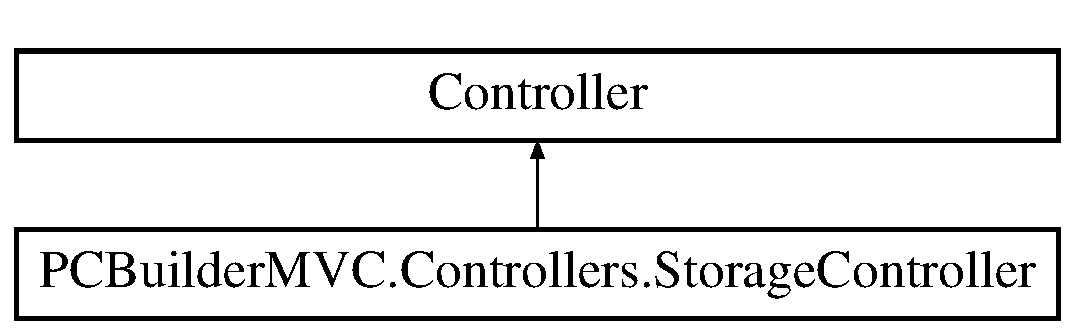
\includegraphics[height=2.000000cm]{class_p_c_builder_m_v_c_1_1_controllers_1_1_storage_controller}
\end{center}
\end{figure}
\subsection*{Public Member Functions}
\begin{DoxyCompactItemize}
\item 
Action\+Result {\bfseries Index} ()\hypertarget{class_p_c_builder_m_v_c_1_1_controllers_1_1_storage_controller_a545a7718bc091a62a8616bc775db274b}{}\label{class_p_c_builder_m_v_c_1_1_controllers_1_1_storage_controller_a545a7718bc091a62a8616bc775db274b}

\item 
Action\+Result {\bfseries Details} (int?id)\hypertarget{class_p_c_builder_m_v_c_1_1_controllers_1_1_storage_controller_a4d127ebd20dad7db886ca02ebdf3de79}{}\label{class_p_c_builder_m_v_c_1_1_controllers_1_1_storage_controller_a4d127ebd20dad7db886ca02ebdf3de79}

\item 
Action\+Result {\bfseries Create} ()\hypertarget{class_p_c_builder_m_v_c_1_1_controllers_1_1_storage_controller_a066b849b419e238c561a2bfd1941d66f}{}\label{class_p_c_builder_m_v_c_1_1_controllers_1_1_storage_controller_a066b849b419e238c561a2bfd1941d66f}

\item 
Action\+Result {\bfseries Create} (\mbox{[}Bind(Include=\char`\"{}Storage\+Id,Brand,Model,Storage\+Size,Storage\+Type,Benchmark\+Score,Storage\+Sequential\+Read,Storage\+Sequential\+Write,Storage\+Random\+Read,Storage\+Random\+Write,Best\+Use,Price\char`\"{})\mbox{]} Storage storage)\hypertarget{class_p_c_builder_m_v_c_1_1_controllers_1_1_storage_controller_a2db58dc1d934110e60e558e4ee38fa21}{}\label{class_p_c_builder_m_v_c_1_1_controllers_1_1_storage_controller_a2db58dc1d934110e60e558e4ee38fa21}

\item 
Action\+Result {\bfseries Edit} (int?id)\hypertarget{class_p_c_builder_m_v_c_1_1_controllers_1_1_storage_controller_ac2c5d09f67d8b57ee5fcb692c641b81a}{}\label{class_p_c_builder_m_v_c_1_1_controllers_1_1_storage_controller_ac2c5d09f67d8b57ee5fcb692c641b81a}

\item 
Action\+Result {\bfseries Edit} (\mbox{[}Bind(Include=\char`\"{}Storage\+Id,Brand,Model,Storage\+Size,Storage\+Type,Benchmark\+Score,Storage\+Sequential\+Read,Storage\+Sequential\+Write,Storage\+Random\+Read,Storage\+Random\+Write,Best\+Use,Price\char`\"{})\mbox{]} Storage storage)\hypertarget{class_p_c_builder_m_v_c_1_1_controllers_1_1_storage_controller_a9997b8e8da2922dcc862fb7af42bd3b6}{}\label{class_p_c_builder_m_v_c_1_1_controllers_1_1_storage_controller_a9997b8e8da2922dcc862fb7af42bd3b6}

\item 
Action\+Result {\bfseries Delete} (int?id)\hypertarget{class_p_c_builder_m_v_c_1_1_controllers_1_1_storage_controller_a61ceedb8611f731f1ce504a3eef2501c}{}\label{class_p_c_builder_m_v_c_1_1_controllers_1_1_storage_controller_a61ceedb8611f731f1ce504a3eef2501c}

\item 
Action\+Result {\bfseries Delete\+Confirmed} (int id)\hypertarget{class_p_c_builder_m_v_c_1_1_controllers_1_1_storage_controller_a18152d71e23f19834e73f8cc958a6f57}{}\label{class_p_c_builder_m_v_c_1_1_controllers_1_1_storage_controller_a18152d71e23f19834e73f8cc958a6f57}

\end{DoxyCompactItemize}
\subsection*{Protected Member Functions}
\begin{DoxyCompactItemize}
\item 
override void {\bfseries Dispose} (bool disposing)\hypertarget{class_p_c_builder_m_v_c_1_1_controllers_1_1_storage_controller_a0c273911b28a7a4d9368775d9a7cc007}{}\label{class_p_c_builder_m_v_c_1_1_controllers_1_1_storage_controller_a0c273911b28a7a4d9368775d9a7cc007}

\end{DoxyCompactItemize}
\subsection*{Private Attributes}
\begin{DoxyCompactItemize}
\item 
\hyperlink{class_p_c_builder_m_v_c_1_1_models_1_1_p_c_builder_entity_models}{P\+C\+Builder\+Entity\+Models} {\bfseries db} = new \hyperlink{class_p_c_builder_m_v_c_1_1_models_1_1_p_c_builder_entity_models}{P\+C\+Builder\+Entity\+Models}()\hypertarget{class_p_c_builder_m_v_c_1_1_controllers_1_1_storage_controller_a446bccc2eff7a3c754f90e65b5aecde9}{}\label{class_p_c_builder_m_v_c_1_1_controllers_1_1_storage_controller_a446bccc2eff7a3c754f90e65b5aecde9}

\end{DoxyCompactItemize}


\subsection{Detailed Description}
Storage controller class to handle Storage views interaction. 

\begin{DoxySeeAlso}{See also}
System.\+Web.\+Mvc.\+Controller


\end{DoxySeeAlso}


Definition at line 17 of file Storage\+Controller.\+cs.



The documentation for this class was generated from the following file\+:\begin{DoxyCompactItemize}
\item 
C\+:/\+Users/nh228u08/\+Desktop/\+Final\+Project/\+Final\+Project/\+P\+C\+Builder/\+P\+C\+Builder\+M\+V\+C/\+Controllers/Storage\+Controller.\+cs\end{DoxyCompactItemize}

\hypertarget{class_p_c_builder_m_v_c_1_1_models_1_1_user}{}\section{P\+C\+Builder\+M\+V\+C.\+Models.\+User Class Reference}
\label{class_p_c_builder_m_v_c_1_1_models_1_1_user}\index{P\+C\+Builder\+M\+V\+C.\+Models.\+User@{P\+C\+Builder\+M\+V\+C.\+Models.\+User}}


\hyperlink{class_p_c_builder_m_v_c_1_1_models_1_1_user}{User} view model class.  


\subsection*{Properties}
\begin{DoxyCompactItemize}
\item 
int {\bfseries User\+Id}\hspace{0.3cm}{\ttfamily  \mbox{[}get, set\mbox{]}}\hypertarget{class_p_c_builder_m_v_c_1_1_models_1_1_user_a5e64dcf76dc09943ccf7c6794e337279}{}\label{class_p_c_builder_m_v_c_1_1_models_1_1_user_a5e64dcf76dc09943ccf7c6794e337279}

\item 
string {\bfseries First\+Name}\hspace{0.3cm}{\ttfamily  \mbox{[}get, set\mbox{]}}\hypertarget{class_p_c_builder_m_v_c_1_1_models_1_1_user_a390fa2a7b3c2c92751420eb4381531f5}{}\label{class_p_c_builder_m_v_c_1_1_models_1_1_user_a390fa2a7b3c2c92751420eb4381531f5}

\item 
string {\bfseries Last\+Name}\hspace{0.3cm}{\ttfamily  \mbox{[}get, set\mbox{]}}\hypertarget{class_p_c_builder_m_v_c_1_1_models_1_1_user_a6afadce146ce780f16ec9e4c8f84b5c4}{}\label{class_p_c_builder_m_v_c_1_1_models_1_1_user_a6afadce146ce780f16ec9e4c8f84b5c4}

\item 
string {\bfseries Address}\hspace{0.3cm}{\ttfamily  \mbox{[}get, set\mbox{]}}\hypertarget{class_p_c_builder_m_v_c_1_1_models_1_1_user_a33910f815ef59234cbcc27bf500e867d}{}\label{class_p_c_builder_m_v_c_1_1_models_1_1_user_a33910f815ef59234cbcc27bf500e867d}

\item 
string {\bfseries City}\hspace{0.3cm}{\ttfamily  \mbox{[}get, set\mbox{]}}\hypertarget{class_p_c_builder_m_v_c_1_1_models_1_1_user_af8302db4cc634f8644c5ed07a270b34b}{}\label{class_p_c_builder_m_v_c_1_1_models_1_1_user_af8302db4cc634f8644c5ed07a270b34b}

\item 
string {\bfseries State\+Code}\hspace{0.3cm}{\ttfamily  \mbox{[}get, set\mbox{]}}\hypertarget{class_p_c_builder_m_v_c_1_1_models_1_1_user_a53a81b7a1ebd76edeb233d5045f378bc}{}\label{class_p_c_builder_m_v_c_1_1_models_1_1_user_a53a81b7a1ebd76edeb233d5045f378bc}

\item 
string {\bfseries Zip}\hspace{0.3cm}{\ttfamily  \mbox{[}get, set\mbox{]}}\hypertarget{class_p_c_builder_m_v_c_1_1_models_1_1_user_ab2e68ef58329fe83dc95b496da154afc}{}\label{class_p_c_builder_m_v_c_1_1_models_1_1_user_ab2e68ef58329fe83dc95b496da154afc}

\item 
string {\bfseries Local\+Phone}\hspace{0.3cm}{\ttfamily  \mbox{[}get, set\mbox{]}}\hypertarget{class_p_c_builder_m_v_c_1_1_models_1_1_user_a386b25c2466543821219255455b2d3e5}{}\label{class_p_c_builder_m_v_c_1_1_models_1_1_user_a386b25c2466543821219255455b2d3e5}

\item 
string {\bfseries Email\+Address}\hspace{0.3cm}{\ttfamily  \mbox{[}get, set\mbox{]}}\hypertarget{class_p_c_builder_m_v_c_1_1_models_1_1_user_a7842479d49253d631bed7e5bb3ac1594}{}\label{class_p_c_builder_m_v_c_1_1_models_1_1_user_a7842479d49253d631bed7e5bb3ac1594}

\item 
string {\bfseries Username}\hspace{0.3cm}{\ttfamily  \mbox{[}get, set\mbox{]}}\hypertarget{class_p_c_builder_m_v_c_1_1_models_1_1_user_af0395972be87058e38df9735b3aec431}{}\label{class_p_c_builder_m_v_c_1_1_models_1_1_user_af0395972be87058e38df9735b3aec431}

\item 
string {\bfseries Password}\hspace{0.3cm}{\ttfamily  \mbox{[}get, set\mbox{]}}\hypertarget{class_p_c_builder_m_v_c_1_1_models_1_1_user_a8bfcb8563ffe3db210b488cd5cae78a2}{}\label{class_p_c_builder_m_v_c_1_1_models_1_1_user_a8bfcb8563ffe3db210b488cd5cae78a2}

\item 
string {\bfseries Role\+Name}\hspace{0.3cm}{\ttfamily  \mbox{[}get, set\mbox{]}}\hypertarget{class_p_c_builder_m_v_c_1_1_models_1_1_user_a8bdf5ce709d4d2bd029d1eb20ab13dfb}{}\label{class_p_c_builder_m_v_c_1_1_models_1_1_user_a8bdf5ce709d4d2bd029d1eb20ab13dfb}

\item 
bool {\bfseries Active}\hspace{0.3cm}{\ttfamily  \mbox{[}get, set\mbox{]}}\hypertarget{class_p_c_builder_m_v_c_1_1_models_1_1_user_a05ce97e1989129db6016b4705b3742f4}{}\label{class_p_c_builder_m_v_c_1_1_models_1_1_user_a05ce97e1989129db6016b4705b3742f4}

\end{DoxyCompactItemize}


\subsection{Detailed Description}
\hyperlink{class_p_c_builder_m_v_c_1_1_models_1_1_user}{User} view model class. 



Definition at line 13 of file User.\+cs.



The documentation for this class was generated from the following file\+:\begin{DoxyCompactItemize}
\item 
C\+:/\+Users/nh228u08/\+Desktop/\+Final\+Project/\+Final\+Project/\+P\+C\+Builder/\+P\+C\+Builder\+M\+V\+C/\+Models/User.\+cs\end{DoxyCompactItemize}

\hypertarget{class_business_objects_1_1_user}{}\section{Business\+Objects.\+User Class Reference}
\label{class_business_objects_1_1_user}\index{Business\+Objects.\+User@{Business\+Objects.\+User}}


\hyperlink{class_business_objects_1_1_user}{User} object to hold necessary data on users.  


Inheritance diagram for Business\+Objects.\+User\+:\begin{figure}[H]
\begin{center}
\leavevmode
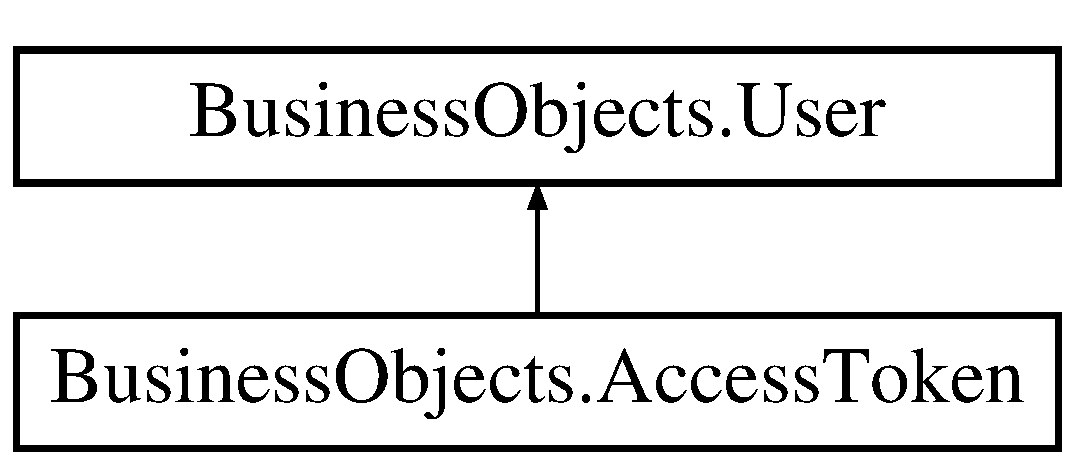
\includegraphics[height=2.000000cm]{class_business_objects_1_1_user}
\end{center}
\end{figure}
\subsection*{Public Member Functions}
\begin{DoxyCompactItemize}
\item 
\hyperlink{class_business_objects_1_1_user_a8fa01831c4b8e4e9d0a9fb6e93b5e2f9}{User} ()
\begin{DoxyCompactList}\small\item\em Initializes a new instance of the \hyperlink{class_business_objects_1_1_user}{User} class. \end{DoxyCompactList}\item 
\hyperlink{class_business_objects_1_1_user_a6a7967d96c26864fb41b03069500eb46}{User} (int user\+ID, string first\+Name, string last\+Name, string address, string city, string state, string zip, string local\+Phone, string email\+Address, string user\+Name, string password, bool active, string role)
\begin{DoxyCompactList}\small\item\em Initializes a new instance of the \hyperlink{class_business_objects_1_1_user}{User} class. \end{DoxyCompactList}\end{DoxyCompactItemize}
\subsection*{Properties}
\begin{DoxyCompactItemize}
\item 
int {\bfseries User\+ID}\hspace{0.3cm}{\ttfamily  \mbox{[}get, set\mbox{]}}\hypertarget{class_business_objects_1_1_user_a0d59552a8aa6580afe57ab02c3c58f9d}{}\label{class_business_objects_1_1_user_a0d59552a8aa6580afe57ab02c3c58f9d}

\item 
string {\bfseries First\+Name}\hspace{0.3cm}{\ttfamily  \mbox{[}get, set\mbox{]}}\hypertarget{class_business_objects_1_1_user_a8206fa75c9fa7057103011bf5379ffc5}{}\label{class_business_objects_1_1_user_a8206fa75c9fa7057103011bf5379ffc5}

\item 
string {\bfseries Last\+Name}\hspace{0.3cm}{\ttfamily  \mbox{[}get, set\mbox{]}}\hypertarget{class_business_objects_1_1_user_af5ae131f690a317df575f57e445a7493}{}\label{class_business_objects_1_1_user_af5ae131f690a317df575f57e445a7493}

\item 
string {\bfseries Address}\hspace{0.3cm}{\ttfamily  \mbox{[}get, set\mbox{]}}\hypertarget{class_business_objects_1_1_user_a17dfee1c4b7764be920621670ac50453}{}\label{class_business_objects_1_1_user_a17dfee1c4b7764be920621670ac50453}

\item 
string {\bfseries City}\hspace{0.3cm}{\ttfamily  \mbox{[}get, set\mbox{]}}\hypertarget{class_business_objects_1_1_user_a659b7c0249dc08fc62020a5a861cb428}{}\label{class_business_objects_1_1_user_a659b7c0249dc08fc62020a5a861cb428}

\item 
string {\bfseries State}\hspace{0.3cm}{\ttfamily  \mbox{[}get, set\mbox{]}}\hypertarget{class_business_objects_1_1_user_aaa0f17d23d58f8ad772ab57415737950}{}\label{class_business_objects_1_1_user_aaa0f17d23d58f8ad772ab57415737950}

\item 
string {\bfseries Zip}\hspace{0.3cm}{\ttfamily  \mbox{[}get, set\mbox{]}}\hypertarget{class_business_objects_1_1_user_aff33b3f3de04d0bca2d45846e82795a3}{}\label{class_business_objects_1_1_user_aff33b3f3de04d0bca2d45846e82795a3}

\item 
string {\bfseries Local\+Phone}\hspace{0.3cm}{\ttfamily  \mbox{[}get, set\mbox{]}}\hypertarget{class_business_objects_1_1_user_af8541ccaa5d8ea7bd9a9b2ef4be98628}{}\label{class_business_objects_1_1_user_af8541ccaa5d8ea7bd9a9b2ef4be98628}

\item 
string {\bfseries Email\+Address}\hspace{0.3cm}{\ttfamily  \mbox{[}get, set\mbox{]}}\hypertarget{class_business_objects_1_1_user_a41f5ad9be3a1dbc01343ffaf71315580}{}\label{class_business_objects_1_1_user_a41f5ad9be3a1dbc01343ffaf71315580}

\item 
string {\bfseries User\+Name}\hspace{0.3cm}{\ttfamily  \mbox{[}get, set\mbox{]}}\hypertarget{class_business_objects_1_1_user_a3b67463b53401175403f5d992aa0412c}{}\label{class_business_objects_1_1_user_a3b67463b53401175403f5d992aa0412c}

\item 
string {\bfseries Password}\hspace{0.3cm}{\ttfamily  \mbox{[}get, set\mbox{]}}\hypertarget{class_business_objects_1_1_user_abec2ef8d60373887ab9d14219edb41e2}{}\label{class_business_objects_1_1_user_abec2ef8d60373887ab9d14219edb41e2}

\item 
string {\bfseries Role}\hspace{0.3cm}{\ttfamily  \mbox{[}get, set\mbox{]}}\hypertarget{class_business_objects_1_1_user_a6e004323033c69f0d9bfd1d5daf7317f}{}\label{class_business_objects_1_1_user_a6e004323033c69f0d9bfd1d5daf7317f}

\item 
bool {\bfseries Active}\hspace{0.3cm}{\ttfamily  \mbox{[}get, set\mbox{]}}\hypertarget{class_business_objects_1_1_user_aa87073276abad34a1a39176a19fcabc3}{}\label{class_business_objects_1_1_user_aa87073276abad34a1a39176a19fcabc3}

\end{DoxyCompactItemize}


\subsection{Detailed Description}
\hyperlink{class_business_objects_1_1_user}{User} object to hold necessary data on users. 



Definition at line 12 of file User.\+cs.



\subsection{Constructor \& Destructor Documentation}
\index{Business\+Objects\+::\+User@{Business\+Objects\+::\+User}!User@{User}}
\index{User@{User}!Business\+Objects\+::\+User@{Business\+Objects\+::\+User}}
\subsubsection[{\texorpdfstring{User()}{User()}}]{\setlength{\rightskip}{0pt plus 5cm}Business\+Objects.\+User.\+User (
\begin{DoxyParamCaption}
{}
\end{DoxyParamCaption}
)}\hypertarget{class_business_objects_1_1_user_a8fa01831c4b8e4e9d0a9fb6e93b5e2f9}{}\label{class_business_objects_1_1_user_a8fa01831c4b8e4e9d0a9fb6e93b5e2f9}


Initializes a new instance of the \hyperlink{class_business_objects_1_1_user}{User} class. 



Definition at line 31 of file User.\+cs.

\index{Business\+Objects\+::\+User@{Business\+Objects\+::\+User}!User@{User}}
\index{User@{User}!Business\+Objects\+::\+User@{Business\+Objects\+::\+User}}
\subsubsection[{\texorpdfstring{User(int user\+I\+D, string first\+Name, string last\+Name, string address, string city, string state, string zip, string local\+Phone, string email\+Address, string user\+Name, string password, bool active, string role)}{User(int userID, string firstName, string lastName, string address, string city, string state, string zip, string localPhone, string emailAddress, string userName, string password, bool active, string role)}}]{\setlength{\rightskip}{0pt plus 5cm}Business\+Objects.\+User.\+User (
\begin{DoxyParamCaption}
\item[{int}]{user\+ID, }
\item[{string}]{first\+Name, }
\item[{string}]{last\+Name, }
\item[{string}]{address, }
\item[{string}]{city, }
\item[{string}]{state, }
\item[{string}]{zip, }
\item[{string}]{local\+Phone, }
\item[{string}]{email\+Address, }
\item[{string}]{user\+Name, }
\item[{string}]{password, }
\item[{bool}]{active, }
\item[{string}]{role}
\end{DoxyParamCaption}
)}\hypertarget{class_business_objects_1_1_user_a6a7967d96c26864fb41b03069500eb46}{}\label{class_business_objects_1_1_user_a6a7967d96c26864fb41b03069500eb46}


Initializes a new instance of the \hyperlink{class_business_objects_1_1_user}{User} class. 


\begin{DoxyParams}{Parameters}
{\em user\+ID} & The user identifier.\\
\hline
{\em first\+Name} & The first name.\\
\hline
{\em last\+Name} & The last name.\\
\hline
{\em address} & The address.\\
\hline
{\em city} & The city.\\
\hline
{\em state} & The state.\\
\hline
{\em zip} & The zip.\\
\hline
{\em local\+Phone} & The local phone.\\
\hline
{\em email\+Address} & The email address.\\
\hline
{\em user\+Name} & Username for the user.\\
\hline
{\em password} & The password.\\
\hline
{\em active} & if set to {\ttfamily true}, \mbox{[}active\mbox{]}.\\
\hline
{\em role} & The role.\\
\hline
\end{DoxyParams}


Definition at line 49 of file User.\+cs.



The documentation for this class was generated from the following file\+:\begin{DoxyCompactItemize}
\item 
C\+:/\+Users/nh228u08/\+Desktop/\+Final\+Project/\+Final\+Project/\+P\+C\+Builder/\+Business\+Objects/User.\+cs\end{DoxyCompactItemize}

\hypertarget{class_data_access_1_1_user_accessor}{}\section{Data\+Access.\+User\+Accessor Class Reference}
\label{class_data_access_1_1_user_accessor}\index{Data\+Access.\+User\+Accessor@{Data\+Access.\+User\+Accessor}}


Data access class that handles data connections with the Users table.  


\subsection*{Static Public Member Functions}
\begin{DoxyCompactItemize}
\item 
static \hyperlink{class_business_objects_1_1_user}{User} \hyperlink{class_data_access_1_1_user_accessor_a72f9e01c595f36043a8ba0801836ac11}{Retrieve\+User\+By\+Username} (string user\+Name)
\begin{DoxyCompactList}\small\item\em Retrieves the user by username. \end{DoxyCompactList}\item 
static List$<$ \hyperlink{class_business_objects_1_1_roles}{Roles} $>$ \hyperlink{class_data_access_1_1_user_accessor_a452e243ca11dd46f9b5c82daf1b19742}{Retrieve\+Roles\+By\+User\+ID} (string username)
\begin{DoxyCompactList}\small\item\em Retrieves the roles by user identifier. \end{DoxyCompactList}\item 
static int \hyperlink{class_data_access_1_1_user_accessor_a47c06dec23dd7b81b6dad6b1c3a55259}{Find\+User\+By\+Username\+And\+Password} (string username, string password)
\begin{DoxyCompactList}\small\item\em Finds the user by username and password. \end{DoxyCompactList}\item 
static int \hyperlink{class_data_access_1_1_user_accessor_acc5b572bb1f5a1073fbe5cfeb0096b65}{Set\+Password\+For\+Username} (string username, string old\+Password, string new\+Password)
\begin{DoxyCompactList}\small\item\em Sets the password for the given username. \end{DoxyCompactList}\item 
static List$<$ \hyperlink{class_business_objects_1_1_user}{User} $>$ \hyperlink{class_data_access_1_1_user_accessor_a9936ef3d80655a8b9e1c63e9969a3c4d}{Fetch\+User\+List} (\hyperlink{namespace_business_objects_a640a4d136931381578aad0a180173cfc}{Active} group=Active.\+active)
\begin{DoxyCompactList}\small\item\em Fetches a user list. \end{DoxyCompactList}\item 
static int \hyperlink{class_data_access_1_1_user_accessor_a54f85a9514bd475a3d5342d31b10ee97}{Fetch\+User\+Count} (\hyperlink{namespace_business_objects_a640a4d136931381578aad0a180173cfc}{Active} group=Active.\+active)
\begin{DoxyCompactList}\small\item\em Fetches the user count. \end{DoxyCompactList}\item 
static int \hyperlink{class_data_access_1_1_user_accessor_a4718ccfb3e6b1b32557c398de4332bf8}{Insert\+User} (\hyperlink{class_business_objects_1_1_user}{User} usr)
\begin{DoxyCompactList}\small\item\em Inserts a new user. \end{DoxyCompactList}\item 
static int \hyperlink{class_data_access_1_1_user_accessor_a7349fc8c87333785420a2896e4c78540}{Update\+User\+Account} (\hyperlink{class_business_objects_1_1_user}{User} usr)
\begin{DoxyCompactList}\small\item\em Updates the user account. \end{DoxyCompactList}\end{DoxyCompactItemize}


\subsection{Detailed Description}
Data access class that handles data connections with the Users table. 



Definition at line 15 of file User\+Accessor.\+cs.



\subsection{Member Function Documentation}
\index{Data\+Access\+::\+User\+Accessor@{Data\+Access\+::\+User\+Accessor}!Fetch\+User\+Count@{Fetch\+User\+Count}}
\index{Fetch\+User\+Count@{Fetch\+User\+Count}!Data\+Access\+::\+User\+Accessor@{Data\+Access\+::\+User\+Accessor}}
\subsubsection[{\texorpdfstring{Fetch\+User\+Count(\+Active group=\+Active.\+active)}{FetchUserCount(Active group=Active.active)}}]{\setlength{\rightskip}{0pt plus 5cm}static int Data\+Access.\+User\+Accessor.\+Fetch\+User\+Count (
\begin{DoxyParamCaption}
\item[{{\bf Active}}]{group = {\ttfamily Active.active}}
\end{DoxyParamCaption}
)\hspace{0.3cm}{\ttfamily [static]}}\hypertarget{class_data_access_1_1_user_accessor_a54f85a9514bd475a3d5342d31b10ee97}{}\label{class_data_access_1_1_user_accessor_a54f85a9514bd475a3d5342d31b10ee97}


Fetches the user count. 


\begin{DoxyParams}{Parameters}
{\em group} & The active status. Defaults to active if no value is passed.\\
\hline
\end{DoxyParams}
\begin{DoxyReturn}{Returns}
Count of records.
\end{DoxyReturn}


Definition at line 252 of file User\+Accessor.\+cs.

\index{Data\+Access\+::\+User\+Accessor@{Data\+Access\+::\+User\+Accessor}!Fetch\+User\+List@{Fetch\+User\+List}}
\index{Fetch\+User\+List@{Fetch\+User\+List}!Data\+Access\+::\+User\+Accessor@{Data\+Access\+::\+User\+Accessor}}
\subsubsection[{\texorpdfstring{Fetch\+User\+List(\+Active group=\+Active.\+active)}{FetchUserList(Active group=Active.active)}}]{\setlength{\rightskip}{0pt plus 5cm}static List$<${\bf User}$>$ Data\+Access.\+User\+Accessor.\+Fetch\+User\+List (
\begin{DoxyParamCaption}
\item[{{\bf Active}}]{group = {\ttfamily Active.active}}
\end{DoxyParamCaption}
)\hspace{0.3cm}{\ttfamily [static]}}\hypertarget{class_data_access_1_1_user_accessor_a9936ef3d80655a8b9e1c63e9969a3c4d}{}\label{class_data_access_1_1_user_accessor_a9936ef3d80655a8b9e1c63e9969a3c4d}


Fetches a user list. 


\begin{DoxyParams}{Parameters}
{\em group} & The group of users. Defaults to active users only.\\
\hline
\end{DoxyParams}
\begin{DoxyReturn}{Returns}
List of Users
\end{DoxyReturn}


Definition at line 195 of file User\+Accessor.\+cs.

\index{Data\+Access\+::\+User\+Accessor@{Data\+Access\+::\+User\+Accessor}!Find\+User\+By\+Username\+And\+Password@{Find\+User\+By\+Username\+And\+Password}}
\index{Find\+User\+By\+Username\+And\+Password@{Find\+User\+By\+Username\+And\+Password}!Data\+Access\+::\+User\+Accessor@{Data\+Access\+::\+User\+Accessor}}
\subsubsection[{\texorpdfstring{Find\+User\+By\+Username\+And\+Password(string username, string password)}{FindUserByUsernameAndPassword(string username, string password)}}]{\setlength{\rightskip}{0pt plus 5cm}static int Data\+Access.\+User\+Accessor.\+Find\+User\+By\+Username\+And\+Password (
\begin{DoxyParamCaption}
\item[{string}]{username, }
\item[{string}]{password}
\end{DoxyParamCaption}
)\hspace{0.3cm}{\ttfamily [static]}}\hypertarget{class_data_access_1_1_user_accessor_a47c06dec23dd7b81b6dad6b1c3a55259}{}\label{class_data_access_1_1_user_accessor_a47c06dec23dd7b81b6dad6b1c3a55259}


Finds the user by username and password. 


\begin{DoxyParams}{Parameters}
{\em username} & The username.\\
\hline
{\em password} & The password.\\
\hline
\end{DoxyParams}
\begin{DoxyReturn}{Returns}
Row count to signify success or failure.
\end{DoxyReturn}


Definition at line 126 of file User\+Accessor.\+cs.

\index{Data\+Access\+::\+User\+Accessor@{Data\+Access\+::\+User\+Accessor}!Insert\+User@{Insert\+User}}
\index{Insert\+User@{Insert\+User}!Data\+Access\+::\+User\+Accessor@{Data\+Access\+::\+User\+Accessor}}
\subsubsection[{\texorpdfstring{Insert\+User(\+User usr)}{InsertUser(User usr)}}]{\setlength{\rightskip}{0pt plus 5cm}static int Data\+Access.\+User\+Accessor.\+Insert\+User (
\begin{DoxyParamCaption}
\item[{{\bf User}}]{usr}
\end{DoxyParamCaption}
)\hspace{0.3cm}{\ttfamily [static]}}\hypertarget{class_data_access_1_1_user_accessor_a4718ccfb3e6b1b32557c398de4332bf8}{}\label{class_data_access_1_1_user_accessor_a4718ccfb3e6b1b32557c398de4332bf8}


Inserts a new user. 


\begin{DoxyParams}{Parameters}
{\em usr} & The user.\\
\hline
\end{DoxyParams}
\begin{DoxyReturn}{Returns}
Count of records affected.
\end{DoxyReturn}


Definition at line 281 of file User\+Accessor.\+cs.

\index{Data\+Access\+::\+User\+Accessor@{Data\+Access\+::\+User\+Accessor}!Retrieve\+Roles\+By\+User\+ID@{Retrieve\+Roles\+By\+User\+ID}}
\index{Retrieve\+Roles\+By\+User\+ID@{Retrieve\+Roles\+By\+User\+ID}!Data\+Access\+::\+User\+Accessor@{Data\+Access\+::\+User\+Accessor}}
\subsubsection[{\texorpdfstring{Retrieve\+Roles\+By\+User\+I\+D(string username)}{RetrieveRolesByUserID(string username)}}]{\setlength{\rightskip}{0pt plus 5cm}static List$<${\bf Roles}$>$ Data\+Access.\+User\+Accessor.\+Retrieve\+Roles\+By\+User\+ID (
\begin{DoxyParamCaption}
\item[{string}]{username}
\end{DoxyParamCaption}
)\hspace{0.3cm}{\ttfamily [static]}}\hypertarget{class_data_access_1_1_user_accessor_a452e243ca11dd46f9b5c82daf1b19742}{}\label{class_data_access_1_1_user_accessor_a452e243ca11dd46f9b5c82daf1b19742}


Retrieves the roles by user identifier. 


\begin{DoxyParams}{Parameters}
{\em username} & The username.\\
\hline
\end{DoxyParams}
\begin{DoxyReturn}{Returns}
List of roles for the username provided.
\end{DoxyReturn}

\begin{DoxyExceptions}{Exceptions}
{\em System.\+Application\+Exception} & Data not found.\\
\hline
\end{DoxyExceptions}


Definition at line 80 of file User\+Accessor.\+cs.

\index{Data\+Access\+::\+User\+Accessor@{Data\+Access\+::\+User\+Accessor}!Retrieve\+User\+By\+Username@{Retrieve\+User\+By\+Username}}
\index{Retrieve\+User\+By\+Username@{Retrieve\+User\+By\+Username}!Data\+Access\+::\+User\+Accessor@{Data\+Access\+::\+User\+Accessor}}
\subsubsection[{\texorpdfstring{Retrieve\+User\+By\+Username(string user\+Name)}{RetrieveUserByUsername(string userName)}}]{\setlength{\rightskip}{0pt plus 5cm}static {\bf User} Data\+Access.\+User\+Accessor.\+Retrieve\+User\+By\+Username (
\begin{DoxyParamCaption}
\item[{string}]{user\+Name}
\end{DoxyParamCaption}
)\hspace{0.3cm}{\ttfamily [static]}}\hypertarget{class_data_access_1_1_user_accessor_a72f9e01c595f36043a8ba0801836ac11}{}\label{class_data_access_1_1_user_accessor_a72f9e01c595f36043a8ba0801836ac11}


Retrieves the user by username. 


\begin{DoxyParams}{Parameters}
{\em user\+Name} & The username from which to retrieve user data.\\
\hline
\end{DoxyParams}
\begin{DoxyReturn}{Returns}
User object from the supplied username.
\end{DoxyReturn}

\begin{DoxyExceptions}{Exceptions}
{\em System.\+Application\+Exception} & Data not found.\\
\hline
\end{DoxyExceptions}


Definition at line 23 of file User\+Accessor.\+cs.

\index{Data\+Access\+::\+User\+Accessor@{Data\+Access\+::\+User\+Accessor}!Set\+Password\+For\+Username@{Set\+Password\+For\+Username}}
\index{Set\+Password\+For\+Username@{Set\+Password\+For\+Username}!Data\+Access\+::\+User\+Accessor@{Data\+Access\+::\+User\+Accessor}}
\subsubsection[{\texorpdfstring{Set\+Password\+For\+Username(string username, string old\+Password, string new\+Password)}{SetPasswordForUsername(string username, string oldPassword, string newPassword)}}]{\setlength{\rightskip}{0pt plus 5cm}static int Data\+Access.\+User\+Accessor.\+Set\+Password\+For\+Username (
\begin{DoxyParamCaption}
\item[{string}]{username, }
\item[{string}]{old\+Password, }
\item[{string}]{new\+Password}
\end{DoxyParamCaption}
)\hspace{0.3cm}{\ttfamily [static]}}\hypertarget{class_data_access_1_1_user_accessor_acc5b572bb1f5a1073fbe5cfeb0096b65}{}\label{class_data_access_1_1_user_accessor_acc5b572bb1f5a1073fbe5cfeb0096b65}


Sets the password for the given username. 


\begin{DoxyParams}{Parameters}
{\em username} & The username.\\
\hline
{\em old\+Password} & The old password.\\
\hline
{\em new\+Password} & The new password.\\
\hline
\end{DoxyParams}
\begin{DoxyReturn}{Returns}
Row count to signify success or failure.
\end{DoxyReturn}


Definition at line 161 of file User\+Accessor.\+cs.

\index{Data\+Access\+::\+User\+Accessor@{Data\+Access\+::\+User\+Accessor}!Update\+User\+Account@{Update\+User\+Account}}
\index{Update\+User\+Account@{Update\+User\+Account}!Data\+Access\+::\+User\+Accessor@{Data\+Access\+::\+User\+Accessor}}
\subsubsection[{\texorpdfstring{Update\+User\+Account(\+User usr)}{UpdateUserAccount(User usr)}}]{\setlength{\rightskip}{0pt plus 5cm}static int Data\+Access.\+User\+Accessor.\+Update\+User\+Account (
\begin{DoxyParamCaption}
\item[{{\bf User}}]{usr}
\end{DoxyParamCaption}
)\hspace{0.3cm}{\ttfamily [static]}}\hypertarget{class_data_access_1_1_user_accessor_a7349fc8c87333785420a2896e4c78540}{}\label{class_data_access_1_1_user_accessor_a7349fc8c87333785420a2896e4c78540}


Updates the user account. 


\begin{DoxyParams}{Parameters}
{\em usr} & The user.\\
\hline
\end{DoxyParams}
\begin{DoxyReturn}{Returns}
Count of records updated.
\end{DoxyReturn}


Definition at line 324 of file User\+Accessor.\+cs.



The documentation for this class was generated from the following file\+:\begin{DoxyCompactItemize}
\item 
C\+:/\+Users/nh228u08/\+Desktop/\+Final\+Project/\+Final\+Project/\+P\+C\+Builder/\+Data\+Access/User\+Accessor.\+cs\end{DoxyCompactItemize}

\hypertarget{class_p_c_builder_m_v_c_1_1_controllers_1_1_user_controller}{}\section{P\+C\+Builder\+M\+V\+C.\+Controllers.\+User\+Controller Class Reference}
\label{class_p_c_builder_m_v_c_1_1_controllers_1_1_user_controller}\index{P\+C\+Builder\+M\+V\+C.\+Controllers.\+User\+Controller@{P\+C\+Builder\+M\+V\+C.\+Controllers.\+User\+Controller}}


User controller class to handle User views interaction  


Inheritance diagram for P\+C\+Builder\+M\+V\+C.\+Controllers.\+User\+Controller\+:\begin{figure}[H]
\begin{center}
\leavevmode
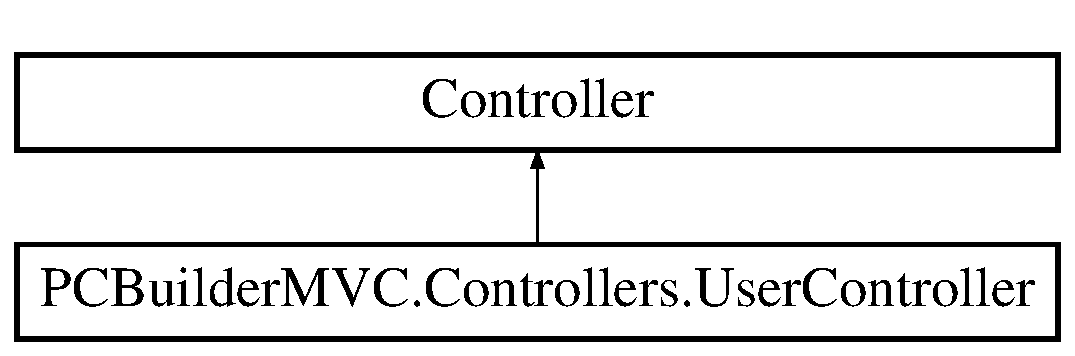
\includegraphics[height=2.000000cm]{class_p_c_builder_m_v_c_1_1_controllers_1_1_user_controller}
\end{center}
\end{figure}
\subsection*{Public Member Functions}
\begin{DoxyCompactItemize}
\item 
Action\+Result {\bfseries Index} ()\hypertarget{class_p_c_builder_m_v_c_1_1_controllers_1_1_user_controller_a2dc3bcfa12cbd3193881110bb2bcf079}{}\label{class_p_c_builder_m_v_c_1_1_controllers_1_1_user_controller_a2dc3bcfa12cbd3193881110bb2bcf079}

\item 
Action\+Result {\bfseries Details} (int?id)\hypertarget{class_p_c_builder_m_v_c_1_1_controllers_1_1_user_controller_ab4bcb8a7721fd91cd6e769a6c5f2111a}{}\label{class_p_c_builder_m_v_c_1_1_controllers_1_1_user_controller_ab4bcb8a7721fd91cd6e769a6c5f2111a}

\item 
Action\+Result {\bfseries Create} ()\hypertarget{class_p_c_builder_m_v_c_1_1_controllers_1_1_user_controller_a018c24eba9f929387f7c426c7799a1a8}{}\label{class_p_c_builder_m_v_c_1_1_controllers_1_1_user_controller_a018c24eba9f929387f7c426c7799a1a8}

\item 
Action\+Result {\bfseries Create} (\mbox{[}Bind(Include=\char`\"{}User\+Id,First\+Name,Last\+Name,Address,City,State\+Code,Zip,Local\+Phone,Email\+Address,Username,Password,Role\+Name,Active\char`\"{})\mbox{]} User user)\hypertarget{class_p_c_builder_m_v_c_1_1_controllers_1_1_user_controller_af8027c377046c4a30aaf6b0c6d80b967}{}\label{class_p_c_builder_m_v_c_1_1_controllers_1_1_user_controller_af8027c377046c4a30aaf6b0c6d80b967}

\item 
Action\+Result {\bfseries Edit} (int?id)\hypertarget{class_p_c_builder_m_v_c_1_1_controllers_1_1_user_controller_a2e149503159c884e4f0cb1c6daca1279}{}\label{class_p_c_builder_m_v_c_1_1_controllers_1_1_user_controller_a2e149503159c884e4f0cb1c6daca1279}

\item 
Action\+Result {\bfseries Edit} (\mbox{[}Bind(Include=\char`\"{}User\+Id,First\+Name,Last\+Name,Address,City,State\+Code,Zip,Local\+Phone,Email\+Address,Username,Password,Role\+Name,Active\char`\"{})\mbox{]} User user)\hypertarget{class_p_c_builder_m_v_c_1_1_controllers_1_1_user_controller_a84cf30a139a0cda5551411ee29654729}{}\label{class_p_c_builder_m_v_c_1_1_controllers_1_1_user_controller_a84cf30a139a0cda5551411ee29654729}

\item 
Action\+Result {\bfseries Delete} (int?id)\hypertarget{class_p_c_builder_m_v_c_1_1_controllers_1_1_user_controller_afeff41f0a91f9d77d4ec0e81471bd649}{}\label{class_p_c_builder_m_v_c_1_1_controllers_1_1_user_controller_afeff41f0a91f9d77d4ec0e81471bd649}

\item 
Action\+Result {\bfseries Delete\+Confirmed} (int id)\hypertarget{class_p_c_builder_m_v_c_1_1_controllers_1_1_user_controller_a6fc23363eff6bad1a8f2f08143d89b60}{}\label{class_p_c_builder_m_v_c_1_1_controllers_1_1_user_controller_a6fc23363eff6bad1a8f2f08143d89b60}

\end{DoxyCompactItemize}
\subsection*{Protected Member Functions}
\begin{DoxyCompactItemize}
\item 
override void {\bfseries Dispose} (bool disposing)\hypertarget{class_p_c_builder_m_v_c_1_1_controllers_1_1_user_controller_af8e537824aef9d778ef7158795528d66}{}\label{class_p_c_builder_m_v_c_1_1_controllers_1_1_user_controller_af8e537824aef9d778ef7158795528d66}

\end{DoxyCompactItemize}
\subsection*{Private Attributes}
\begin{DoxyCompactItemize}
\item 
\hyperlink{class_p_c_builder_m_v_c_1_1_models_1_1_p_c_builder_entity_models}{P\+C\+Builder\+Entity\+Models} {\bfseries db} = new \hyperlink{class_p_c_builder_m_v_c_1_1_models_1_1_p_c_builder_entity_models}{P\+C\+Builder\+Entity\+Models}()\hypertarget{class_p_c_builder_m_v_c_1_1_controllers_1_1_user_controller_a7dd8061d33d8b9a9ca57bf574302a53f}{}\label{class_p_c_builder_m_v_c_1_1_controllers_1_1_user_controller_a7dd8061d33d8b9a9ca57bf574302a53f}

\end{DoxyCompactItemize}


\subsection{Detailed Description}
User controller class to handle User views interaction 

\begin{DoxySeeAlso}{See also}
System.\+Web.\+Mvc.\+Controller


\end{DoxySeeAlso}


Definition at line 17 of file User\+Controller.\+cs.



The documentation for this class was generated from the following file\+:\begin{DoxyCompactItemize}
\item 
C\+:/\+Users/nh228u08/\+Desktop/\+Final\+Project/\+Final\+Project/\+P\+C\+Builder/\+P\+C\+Builder\+M\+V\+C/\+Controllers/User\+Controller.\+cs\end{DoxyCompactItemize}

\hypertarget{class_p_c_builder_m_v_c_1_1_models_1_1_user_entities}{}\section{P\+C\+Builder\+M\+V\+C.\+Models.\+User\+Entities Class Reference}
\label{class_p_c_builder_m_v_c_1_1_models_1_1_user_entities}\index{P\+C\+Builder\+M\+V\+C.\+Models.\+User\+Entities@{P\+C\+Builder\+M\+V\+C.\+Models.\+User\+Entities}}
Inheritance diagram for P\+C\+Builder\+M\+V\+C.\+Models.\+User\+Entities\+:\begin{figure}[H]
\begin{center}
\leavevmode
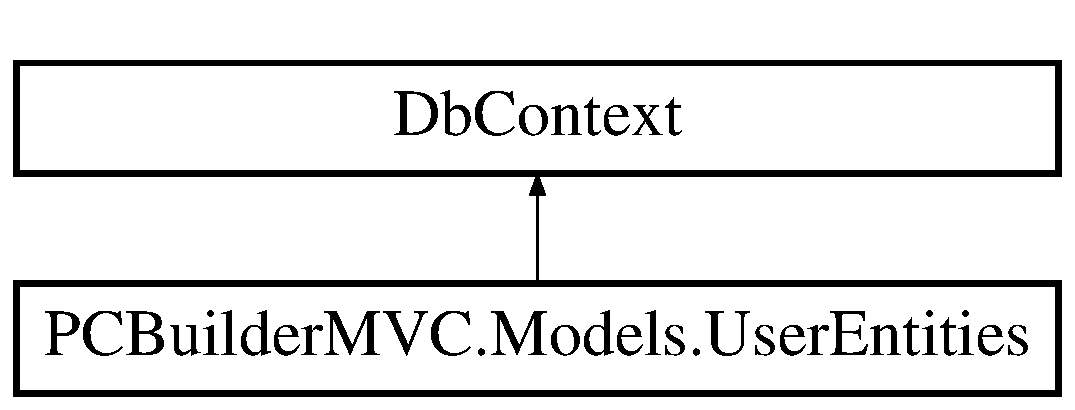
\includegraphics[height=2.000000cm]{class_p_c_builder_m_v_c_1_1_models_1_1_user_entities}
\end{center}
\end{figure}
\subsection*{Protected Member Functions}
\begin{DoxyCompactItemize}
\item 
override void {\bfseries On\+Model\+Creating} (Db\+Model\+Builder model\+Builder)\hypertarget{class_p_c_builder_m_v_c_1_1_models_1_1_user_entities_a4e4635cfa93a11fe54575099f2394030}{}\label{class_p_c_builder_m_v_c_1_1_models_1_1_user_entities_a4e4635cfa93a11fe54575099f2394030}

\end{DoxyCompactItemize}
\subsection*{Properties}
\begin{DoxyCompactItemize}
\item 
virtual Db\+Set$<$ \hyperlink{class_p_c_builder_m_v_c_1_1_models_1_1_asp_net_role}{Asp\+Net\+Role} $>$ {\bfseries Asp\+Net\+Roles}\hspace{0.3cm}{\ttfamily  \mbox{[}get, set\mbox{]}}\hypertarget{class_p_c_builder_m_v_c_1_1_models_1_1_user_entities_a97ad62df5e44eb5d06b4faef97066545}{}\label{class_p_c_builder_m_v_c_1_1_models_1_1_user_entities_a97ad62df5e44eb5d06b4faef97066545}

\item 
virtual Db\+Set$<$ \hyperlink{class_p_c_builder_m_v_c_1_1_models_1_1_asp_net_user_claim}{Asp\+Net\+User\+Claim} $>$ {\bfseries Asp\+Net\+User\+Claims}\hspace{0.3cm}{\ttfamily  \mbox{[}get, set\mbox{]}}\hypertarget{class_p_c_builder_m_v_c_1_1_models_1_1_user_entities_adce18308000a7a93875ade45b503e94e}{}\label{class_p_c_builder_m_v_c_1_1_models_1_1_user_entities_adce18308000a7a93875ade45b503e94e}

\item 
virtual Db\+Set$<$ \hyperlink{class_p_c_builder_m_v_c_1_1_models_1_1_asp_net_user_login}{Asp\+Net\+User\+Login} $>$ {\bfseries Asp\+Net\+User\+Logins}\hspace{0.3cm}{\ttfamily  \mbox{[}get, set\mbox{]}}\hypertarget{class_p_c_builder_m_v_c_1_1_models_1_1_user_entities_ad930890fad3392c62f1915b2baea7f67}{}\label{class_p_c_builder_m_v_c_1_1_models_1_1_user_entities_ad930890fad3392c62f1915b2baea7f67}

\item 
virtual Db\+Set$<$ \hyperlink{class_p_c_builder_m_v_c_1_1_models_1_1_asp_net_user}{Asp\+Net\+User} $>$ {\bfseries Asp\+Net\+Users}\hspace{0.3cm}{\ttfamily  \mbox{[}get, set\mbox{]}}\hypertarget{class_p_c_builder_m_v_c_1_1_models_1_1_user_entities_a0bdbcfd5cd36963f3b56d2a28eee0b59}{}\label{class_p_c_builder_m_v_c_1_1_models_1_1_user_entities_a0bdbcfd5cd36963f3b56d2a28eee0b59}

\end{DoxyCompactItemize}


\subsection{Detailed Description}


Definition at line 16 of file Users.\+Context.\+cs.



The documentation for this class was generated from the following file\+:\begin{DoxyCompactItemize}
\item 
C\+:/\+Users/nh228u08/\+Desktop/\+Final\+Project/\+Final\+Project/\+P\+C\+Builder/\+P\+C\+Builder\+M\+V\+C/\+Models/Users.\+Context.\+cs\end{DoxyCompactItemize}

\hypertarget{class_business_logic_1_1_user_manager}{}\section{Business\+Logic.\+User\+Manager Class Reference}
\label{class_business_logic_1_1_user_manager}\index{Business\+Logic.\+User\+Manager@{Business\+Logic.\+User\+Manager}}


User manager with the job of talking to the database for user fields.  


\subsection*{Public Member Functions}
\begin{DoxyCompactItemize}
\item 
List$<$ \hyperlink{class_business_objects_1_1_user}{User} $>$ \hyperlink{class_business_logic_1_1_user_manager_a3056179e2041b2022e1a28356188c288}{Get\+User\+List} (\hyperlink{namespace_business_objects_a640a4d136931381578aad0a180173cfc}{Active} group)
\begin{DoxyCompactList}\small\item\em Gets the user list for all active users. \end{DoxyCompactList}\item 
int \hyperlink{class_business_logic_1_1_user_manager_a65be32ae93f260d00fc7d259470d8869}{Get\+User\+Count} (\hyperlink{namespace_business_objects_a640a4d136931381578aad0a180173cfc}{Active} group=Active.\+active)
\begin{DoxyCompactList}\small\item\em Gets the user count for all active users. \end{DoxyCompactList}\item 
bool \hyperlink{class_business_logic_1_1_user_manager_ab868aeac2dd021d3d230cceb099422c8}{Add\+New\+User} (\hyperlink{class_business_objects_1_1_user}{User} usr)
\begin{DoxyCompactList}\small\item\em Adds a new user. \end{DoxyCompactList}\item 
bool \hyperlink{class_business_logic_1_1_user_manager_a58674010581be08d264cb486810c9de8}{Update\+User\+Information} (\hyperlink{class_business_objects_1_1_user}{User} usr)
\begin{DoxyCompactList}\small\item\em Updates the user information. \end{DoxyCompactList}\end{DoxyCompactItemize}


\subsection{Detailed Description}
User manager with the job of talking to the database for user fields. 



Definition at line 16 of file User\+Manager.\+cs.



\subsection{Member Function Documentation}
\index{Business\+Logic\+::\+User\+Manager@{Business\+Logic\+::\+User\+Manager}!Add\+New\+User@{Add\+New\+User}}
\index{Add\+New\+User@{Add\+New\+User}!Business\+Logic\+::\+User\+Manager@{Business\+Logic\+::\+User\+Manager}}
\subsubsection[{\texorpdfstring{Add\+New\+User(\+User usr)}{AddNewUser(User usr)}}]{\setlength{\rightskip}{0pt plus 5cm}bool Business\+Logic.\+User\+Manager.\+Add\+New\+User (
\begin{DoxyParamCaption}
\item[{{\bf User}}]{usr}
\end{DoxyParamCaption}
)}\hypertarget{class_business_logic_1_1_user_manager_ab868aeac2dd021d3d230cceb099422c8}{}\label{class_business_logic_1_1_user_manager_ab868aeac2dd021d3d230cceb099422c8}


Adds a new user. 


\begin{DoxyParams}{Parameters}
{\em usr} & The user to be added.\\
\hline
\end{DoxyParams}
\begin{DoxyReturn}{Returns}
Boolean result of the insert.
\end{DoxyReturn}


Definition at line 67 of file User\+Manager.\+cs.

\index{Business\+Logic\+::\+User\+Manager@{Business\+Logic\+::\+User\+Manager}!Get\+User\+Count@{Get\+User\+Count}}
\index{Get\+User\+Count@{Get\+User\+Count}!Business\+Logic\+::\+User\+Manager@{Business\+Logic\+::\+User\+Manager}}
\subsubsection[{\texorpdfstring{Get\+User\+Count(\+Active group=\+Active.\+active)}{GetUserCount(Active group=Active.active)}}]{\setlength{\rightskip}{0pt plus 5cm}int Business\+Logic.\+User\+Manager.\+Get\+User\+Count (
\begin{DoxyParamCaption}
\item[{{\bf Active}}]{group = {\ttfamily Active.active}}
\end{DoxyParamCaption}
)}\hypertarget{class_business_logic_1_1_user_manager_a65be32ae93f260d00fc7d259470d8869}{}\label{class_business_logic_1_1_user_manager_a65be32ae93f260d00fc7d259470d8869}


Gets the user count for all active users. 


\begin{DoxyParams}{Parameters}
{\em group} & The active status. Defaults to active if no value is passed.\\
\hline
\end{DoxyParams}
\begin{DoxyReturn}{Returns}
Count of active users.
\end{DoxyReturn}


Definition at line 50 of file User\+Manager.\+cs.

\index{Business\+Logic\+::\+User\+Manager@{Business\+Logic\+::\+User\+Manager}!Get\+User\+List@{Get\+User\+List}}
\index{Get\+User\+List@{Get\+User\+List}!Business\+Logic\+::\+User\+Manager@{Business\+Logic\+::\+User\+Manager}}
\subsubsection[{\texorpdfstring{Get\+User\+List(\+Active group)}{GetUserList(Active group)}}]{\setlength{\rightskip}{0pt plus 5cm}List$<${\bf User}$>$ Business\+Logic.\+User\+Manager.\+Get\+User\+List (
\begin{DoxyParamCaption}
\item[{{\bf Active}}]{group}
\end{DoxyParamCaption}
)}\hypertarget{class_business_logic_1_1_user_manager_a3056179e2041b2022e1a28356188c288}{}\label{class_business_logic_1_1_user_manager_a3056179e2041b2022e1a28356188c288}


Gets the user list for all active users. 


\begin{DoxyParams}{Parameters}
{\em group} & The group.\\
\hline
\end{DoxyParams}
\begin{DoxyReturn}{Returns}
List of Users.
\end{DoxyReturn}

\begin{DoxyExceptions}{Exceptions}
{\em System.\+Application\+Exception} & No records found.\\
\hline
\end{DoxyExceptions}


Definition at line 24 of file User\+Manager.\+cs.

\index{Business\+Logic\+::\+User\+Manager@{Business\+Logic\+::\+User\+Manager}!Update\+User\+Information@{Update\+User\+Information}}
\index{Update\+User\+Information@{Update\+User\+Information}!Business\+Logic\+::\+User\+Manager@{Business\+Logic\+::\+User\+Manager}}
\subsubsection[{\texorpdfstring{Update\+User\+Information(\+User usr)}{UpdateUserInformation(User usr)}}]{\setlength{\rightskip}{0pt plus 5cm}bool Business\+Logic.\+User\+Manager.\+Update\+User\+Information (
\begin{DoxyParamCaption}
\item[{{\bf User}}]{usr}
\end{DoxyParamCaption}
)}\hypertarget{class_business_logic_1_1_user_manager_a58674010581be08d264cb486810c9de8}{}\label{class_business_logic_1_1_user_manager_a58674010581be08d264cb486810c9de8}


Updates the user information. 


\begin{DoxyParams}{Parameters}
{\em usr} & The user to be updated.\\
\hline
\end{DoxyParams}
\begin{DoxyReturn}{Returns}
Boolean result of the update.
\end{DoxyReturn}

\begin{DoxyExceptions}{Exceptions}
{\em System.\+Application\+Exception} & Invalid user\+ID or First name is too long. Maximum 50 characters. or Last name is too long.\textquotesingle{} Maximum 50 characters. or Address is too long.\textquotesingle{} Maximum 50 characters. or City name is too long.\textquotesingle{} Maximum 50 characters. or User name is too long.\textquotesingle{} Maximum 50 characters. or Email address is too long. Maximun 100 characters. \\
\hline
\end{DoxyExceptions}


Definition at line 104 of file User\+Manager.\+cs.



The documentation for this class was generated from the following file\+:\begin{DoxyCompactItemize}
\item 
C\+:/\+Users/nh228u08/\+Desktop/\+Final\+Project/\+Final\+Project/\+P\+C\+Builder/\+Business\+Logic/User\+Manager.\+cs\end{DoxyCompactItemize}

\hypertarget{class_p_c_builder_forms_1_1_window1}{}\section{P\+C\+Builder\+Forms.\+Window1 Class Reference}
\label{class_p_c_builder_forms_1_1_window1}\index{P\+C\+Builder\+Forms.\+Window1@{P\+C\+Builder\+Forms.\+Window1}}


\hyperlink{class_p_c_builder_forms_1_1_window1}{Window1}  


Inheritance diagram for P\+C\+Builder\+Forms.\+Window1\+:\begin{figure}[H]
\begin{center}
\leavevmode
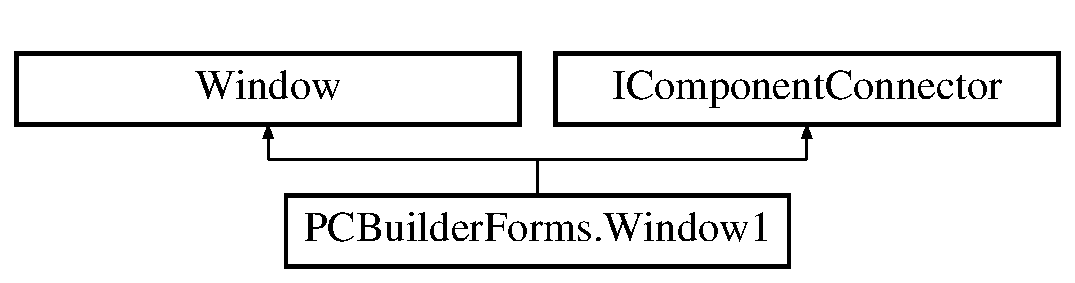
\includegraphics[height=2.000000cm]{class_p_c_builder_forms_1_1_window1}
\end{center}
\end{figure}
\subsection*{Public Member Functions}
\begin{DoxyCompactItemize}
\item 
void \hyperlink{class_p_c_builder_forms_1_1_window1_a5cda1cb9593c778c04476a1584714a4c}{Initialize\+Component} ()
\begin{DoxyCompactList}\small\item\em Initialize\+Component \end{DoxyCompactList}\end{DoxyCompactItemize}
\subsection*{Private Member Functions}
\begin{DoxyCompactItemize}
\item 
void System.\+Windows.\+Markup.\+I\+Component\+Connector. {\bfseries Connect} (int connection\+Id, object target)\hypertarget{class_p_c_builder_forms_1_1_window1_a0540083e435f2a48f9cbc604ffaffff4}{}\label{class_p_c_builder_forms_1_1_window1_a0540083e435f2a48f9cbc604ffaffff4}

\end{DoxyCompactItemize}
\subsection*{Private Attributes}
\begin{DoxyCompactItemize}
\item 
bool {\bfseries \+\_\+content\+Loaded}\hypertarget{class_p_c_builder_forms_1_1_window1_a31e5fc9ff6f8e2ad6453b364c986175d}{}\label{class_p_c_builder_forms_1_1_window1_a31e5fc9ff6f8e2ad6453b364c986175d}

\end{DoxyCompactItemize}


\subsection{Detailed Description}
\hyperlink{class_p_c_builder_forms_1_1_window1}{Window1} 



Definition at line 40 of file Window1.\+g.\+i.\+cs.



\subsection{Member Function Documentation}
\index{P\+C\+Builder\+Forms\+::\+Window1@{P\+C\+Builder\+Forms\+::\+Window1}!Initialize\+Component@{Initialize\+Component}}
\index{Initialize\+Component@{Initialize\+Component}!P\+C\+Builder\+Forms\+::\+Window1@{P\+C\+Builder\+Forms\+::\+Window1}}
\subsubsection[{\texorpdfstring{Initialize\+Component()}{InitializeComponent()}}]{\setlength{\rightskip}{0pt plus 5cm}void P\+C\+Builder\+Forms.\+Window1.\+Initialize\+Component (
\begin{DoxyParamCaption}
{}
\end{DoxyParamCaption}
)}\hypertarget{class_p_c_builder_forms_1_1_window1_a5cda1cb9593c778c04476a1584714a4c}{}\label{class_p_c_builder_forms_1_1_window1_a5cda1cb9593c778c04476a1584714a4c}


Initialize\+Component 



Definition at line 49 of file Window1.\+g.\+i.\+cs.



The documentation for this class was generated from the following file\+:\begin{DoxyCompactItemize}
\item 
C\+:/\+Users/nh228u08/\+Desktop/\+Final\+Project/\+Final\+Project/\+P\+C\+Builder/\+P\+C\+Builder\+Forms/obj/\+Debug/Window1.\+g.\+i.\+cs\end{DoxyCompactItemize}

%--- End generated contents ---

% Index
\backmatter
\newpage
\phantomsection
\clearemptydoublepage
\addcontentsline{toc}{chapter}{Index}
\printindex

\end{document}
